% !TeX spellcheck = es_ES
% !TeX encoding = ISO-8859-1

\documentclass[letterpaper,titlepage,12pt,oneside,spanish,final]{report_eie}

%\documentclass[letterpaper,titlepage,12pt,twoside,openright,spanish,final]{report_eie}

%%%%%%%%%%%%%%%%%%%%%%%%%%%%%%%%%%%%%%%%%%%%%%%%%%%%%%%%%%%%%%%%%%%%%%%%
\usepackage[spanish]{babel}
%\usepackage[latin1]{inputenc}
\usepackage[utf8]{inputenc} %Reconoce tildes y otros simbolos propios del espa?ol
\usepackage[T1]{fontenc}  %Estilo de fuente time new roman

\usepackage{amssymb}
\usepackage{amsfonts}
\usepackage{amsmath}
\usepackage{latexsym}
\usepackage[letterpaper]{geometry}

\usepackage{float}
\usepackage{makeidx}
\usepackage{color}

\usepackage{tocbibind}
\usepackage{acronym}
%\usepackage{caption2}
\usepackage{epsfig}
\usepackage{graphicx}
\usepackage{slashbox}
\usepackage{setspace}
\usepackage{multicol}
\usepackage{longtable}
%\usepackage{doublespace}

\usepackage{fancyhdr}
%\usepackage{fancyheadings}

\usepackage{booktabs}



%========= Define el estilo de referencias ===============
%\usepackage[round,authoryear]{natbib}%\usepackage[square,numbers]{natbib}%
%\usepackage[comma,authoryear]{natbib} esto est? abajo

%========= Define el estilo de referencias APA ===============
%\usepackage[natbibapa]{apacite}%natbibapa
\usepackage[numbers]{natbib}%natbibapa
%\usepackage[apaciteclassic]{apacite}%natbibapa
%\usepackage[compact]{titlesec} %modificar espaciado


\usepackage{url}
%\usepackage{hyperref}
\usepackage[colorlinks=true,urlcolor=black,citecolor=black,anchorcolor=black,linkcolor=black]{hyperref}

\usepackage{adjustbox}

\UseRawInputEncoding

%%%%%%%%%%%%%%%%%%%%%%%%%%%%%%%%%%%%%%%%%%%%%%%%%%%%%%%%%%%%%%%%%%
%            Definici?n del Documento PDF, (PDFLaTeX)            %
%%%%%%%%%%%%%%%%%%%%%%%%%%%%%%%%%%%%%%%%%%%%%%%%%%%%%%%%%%%%%%%%%%

\hypersetup{pdfauthor=Nombre}

\hypersetup{pdftitle=T�tulo}%

\hypersetup{pdfkeywords=Palabras clave}

\pdfstringdef{\Produce}{Escuela de Ingenier�a El�ctrica, Facultad de Ingenier�a, UCV}%

\pdfstringdef{\area}{�rea del trabajo}

\hypersetup{pdfproducer=\Produce}

\hypersetup{pdfsubject=\area}

\hypersetup{bookmarksnumbered=true}

%%%%%%%%%%%%%%%%%%%%%%%%%%%%%%%%%%%%%%%%%%%%%%%%%%%%%%%%%%%%%%%%%%

%%%%%%%%%%%%%%%%%%%%%%%%%%%%%%%%%%%%%%%%%%%%%%%%%%%%%%%%%%%%%%%%
%Source in images
\newcommand*{\captionsource}[2]{%
	\caption[{#1}]{%
		#1%
		\\%
		\textbf{Fuente:} #2%
	}%
}
%%%%%%%%%%%%%%%%%%%%%%%%%%%%%%%%%%%%%%%%%%%%%%%%%%%%%%%%%%%%%%%%%


%\setcounter{MaxMatrixCols}{10}


%===================== Re-definici?n de Ambientes =================
\newtheorem{theorem}{Teorema}
\newtheorem{acknowledgement}[theorem]{Acknowledgement}
\newtheorem{algoritmo}[theorem]{Algorithm}
\newtheorem{supuestos}[theorem]{Supuestos}
\newtheorem{hipotesis}[theorem]{Hip�tesis}
\newtheorem{axiom}[theorem]{Axiom}
\newtheorem{case}[theorem]{Case}
\newtheorem{claim}[theorem]{Claim}
\newtheorem{conclusion}[theorem]{Conclusi�n}
\newtheorem{condition}{Condici�n}
\newtheorem{conjecture}{Conjecture}
\newtheorem{corollary}{Corollary}
\newtheorem{criterion}{Criterion}
\newtheorem{definition}{Definici�n}  %{Definition}
\newtheorem{example}[theorem]{Ejemplo}%{Example}
\newtheorem{exercise}[theorem]{Exercise}
\newtheorem{lemma}{Lemma}
\newtheorem{notation}[theorem]{Notation}
\newtheorem{problem}{Problem}
\newtheorem{property}{Property}
\newtheorem{proposition}{Proposition}
\newtheorem{remark}[theorem]{Remark}
\newtheorem{solution}{Solution}
\newtheorem{summary}[theorem]{Summary}
\newenvironment{proof}[1][Proof]{\noindent\textbf{#1.} }{\ \rule{0.5em}{0.5em}}%

\numberwithin{equation}{chapter}%
\numberwithin{figure}{chapter}%
\numberwithin{table}{chapter}%
\numberwithin{definition}{chapter}%
\numberwithin{lemma}{chapter}%
\numberwithin{theorem}{chapter}%
\numberwithin{corollary}{chapter}%
\numberwithin{condition}{chapter}%
\numberwithin{criterion}{chapter}%
 \numberwithin{problem}{chapter}%
\numberwithin{property}{chapter}%
\numberwithin{proposition}{chapter}%
\numberwithin{solution}{chapter}%
\numberwithin{conjecture}{chapter}%

%==================== Separaci?n en s?labas ========================
\hyphenpenalty=6800%

%A
\hyphenation{a-pro-xi-ma-do}


%B
\hyphenation{ba-lan-ce}%

%C
\hyphenation{co-la-bo-ra-do-res}%
\hyphenation{co-rres-pon-dien-tes}%
\hyphenation{co-rres-pon-dien-te}%
\hyphenation{con-ti-nua-men-te}%
\hyphenation{con-si-de-ra-cio-nes}%
\hyphenation{cons-tru-ir}%
\hyphenation{con-si-de-ra-do}%


%D
\hyphenation{di-fe-ren-cia}%
\hyphenation{des-cri-tos}%
\hyphenation{dis-mi-nu-ye}%
\hyphenation{des-cri-to}%
\hyphenation{de-pen-dien-tes}%


%E
\hyphenation{ex-pe-ri-men-to}
\hyphenation{ex-pe-ri-men-ta-cion} %


%P
\hyphenation{pro-ba-bi-li-da-des}%
\hyphenation{pro-ba-bi-li-dad}%
\hyphenation{par-ti-cu-lar}%

%M
\hyphenation{mo-da-li-da-des}%
\hyphenation{mo-de-lo} %
\hyphenation{me-dian-te}%
 \hyphenation{man-te-ni-mien-tos}%
%N

%O
\hyphenation{ope-ra-cio-nal}%
\hyphenation{o-pe-ra-cion}%
\hyphenation{o-pe-ra-cio-nes} %
\hyphenation{o-pe-ra-do-ra}%


%==================== Dise?o de P?gina =============================
%\pagestyle{headings}
%\setlength{\headheight}{0.2cm}
\setlength{\textwidth}{14.52cm}%
%\pagestyle{fancy}
\renewcommand{\chaptermark}[1]{\markboth{#1}{}}
%\renewcommand{\sectionmark}[1]{\markright{\thesection\ #1}}
%\rhead[\fancyplain{}{\bfseries\thepage}]{\fancyplain{}{\bfseries\rightmark}}%\thepage
%\lhead[\fancyplain{}{\bfseries\leftmark}]{\fancyplain{}{\bfseries}} \cfoot{}%

%\fancyhead[R]{}


\rfoot[\fancyplain{}{\textit{M. Rodr�guez}}] {\fancyplain{}{}}
\lfoot[\fancyplain{}{}] {\fancyplain{}{\textit{}}}    %%%%%%%%%%%%%%%%%%% OJO ACA %%%%%%%%%%
\cfoot[\fancyplain{}{}] {\fancyplain{}{\bfseries\thepage}}
%\setlength{\footrulewidth}{0.0pt}%
%\setlength{\headrulewidth}{0.1pt}%

%===================================================================



%================== Dise?o de P?rrafo y delimitador ================
\renewcommand{\baselinestretch}{1.5}% Espaciado entre linea
\geometry{left=4cm,right=3cm,top=3cm,bottom=3cm}
\frenchspacing %
%\raggedright % S?lo para justificar el texto a la izquierda
%\renewcommand{\captionlabeldelim}{.}%
\setlength{\parindent}{0.7cm}% Espacio de la sangr?a
\setlength{\parskip}{14pt plus 1pt minus 1pt}% Separaci?n entre p?rrafos

%\setlength{\parskip}{1ex plus 0.5ex minus 0.2ex}%


%===================================================================

%==========================  Espa?ol venezolano =====================
%%Personalizaci?n de caption
\addto\captionsspanish{%
  \def\prefacename{Prefacio}%
  \def\refname{REFERENCIAS}%
  \def\abstractname{Resumen}%
  \def\bibname{REFERENCIAS}%{Bibliograf?a}%
  \def\chaptername{CAP�TULO}%
  \def\appendixname{Ap�ndice}%{Anexo}
  \def\contentsname{�NDICE GENERAL}
  \def\listfigurename{LISTA DE FIGURAS}%?ndice de Figuras\hspace*{10em}
  \def\listfigurenameTofC{LISTA DE FIGURAS}%?ndice de Figuras
  \def\listtablename{LISTA DE TABLAS}%?ndice de Tablas
  \def\indexname{�ndice alfab�tico}%
  \def\figurename{Figura}%
  \def\tablename{Tabla}%
  \def\partname{Parte}%
  \def\enclname{Adjunto}%
  \def\ccname{Copia a}%
  \def\headtoname{A}%
  \def\pagename{P�gina}%
  \def\seename{v�ase}%
  \def\alsoname{v�ase tambi�n}%
  \def\proofname{Demostraci�n}%
  \def\glossaryname{Glosario}
  }%


%%%%%%%%%%%%%%%%%%%%%%%%%%%%%%%%%%%%%%%%%%%%%%%%%%%%%%%%%%%%%%%%%%
%            Anexo de codigo y pseudocodigo				         %
%%%%%%%%%%%%%%%%%%%%%%%%%%%%%%%%%%%%%%%%%%%%%%%%%%%%%%%%%%%%%%%%%%
\usepackage{amssymb,latexsym,amsmath}
\usepackage{setspace}
\usepackage[table,dvipsnames,x11names,svgnames]{xcolor}
\usepackage[skins,theorems,listings,breakable]{tcolorbox}
\usepackage{listings}
\usepackage{geometry}
\geometry{top=1.5cm,bottom=1.5cm,left=2.5cm,right=2.5cm}
\usepackage{graphicx}

\pagestyle{empty}

\def\lstlistingname{Programa}%  Aqu� puedes cambiar el nombre del t�tulo del listado
%Listing

\definecolor{comentario}{rgb}{0.68,0.68,0.68}%\textcolor[rgb]{0.68,0.68,0.68}{}
\definecolor{cadena}{rgb}{0.00,0.67,0.00}%\textcolor[rgb]{0.00,0.67,0.00}{}
\definecolor{keywords}{rgb}{0.00,0.00,1.00}%\textcolor[rgb]{0.00,0.00,1.00}{}
\definecolor{Decorators}{rgb}{0.5,0.5,0.5}%
\definecolor{objeto_integrado}{rgb}{0.56,0.00,0.56}%\textcolor[rgb]{0.56,0.00,0.56}{}

\lstdefinelanguage{Python}{
	showspaces=false,
	showtabs=false,
	showstringspaces=false,
	tabsize=4,
	% Basic
	basicstyle=\footnotesize\setstretch{1},
	% Comments
	commentstyle=\color{comentario},
	% Strings
	stringstyle=\color{cadena},
	morestring=[b]',
	morecomment=[s][\color{cadena}]{"""}{"""},
	morecomment=[s][\color{cadena}]{'''}{'''},
	morecomment=[l]\#,
	% keywords
	morekeywords={import,from,class,def,for,while,if,is,in,elif,else,not,and,or,break,continue,return,access,as,del,except,finally,global,import,lambda,pass,raise,try,assert},
	keywordstyle={\color{keywords}},
	%additional keywords
	morekeywords={[2]@invariant,print,True,False,None,exec,len},
	keywordstyle={[2]\color{objeto_integrado}},
	otherkeywords={>>>},
	morekeywords=[3]{>>>},
	keywordstyle={[3]\footnotesize\ttfamily\color{DarkOrange}}
}

\tcbset{
	program/.style={
		width=.95\textwidth,
		enlarge left by=.05\textwidth,
		enlarge right by=-.05\textwidth,
		colframe=Black,
		colback=white,
		fonttitle=\small\sffamily\bfseries,
		fontupper=\small,
		fontlower=\small,
		breakable,
		listing only,
		size=small,
		enhanced,
		attach boxed title to top center,
		fonttitle=\rm,coltitle=black,
		boxed title style={size=small,colback=white,colframe=white},
		beforeafter skip=9pt,
		listing options={language=Python}},
	listado/.style 2 args={program, title={{\bf Programa~\thetcbcounter.} #1},label={#2}}
}
\newtcblisting{program}[1]{modulo,#1}
\newtcblisting[auto counter]{programa}[3][]{listado={#2}{#3},#1}

%==================================================================

%\setcounter{secnumdepth}{1}
%\setcounter{page}{4}
%\addtocounter{page}{4}%

\pagenumbering{roman}

\makeindex


%%%%%%%%%%%%%%%%%%%%%%%%%%%%%%%%%%%%%%%%%%%%%%%%%%%%%%%%%%%%%%%%%

\begin{document}
%\frontmatter

%====================Math ==============================
\def\vectornu{\mathbf{v}}%)\,)
\def\sen{\mathrm{sen}}
%\def\cos{\mathrm{cos}}
%\def\vectornu2{\nu_{n}}

%===================================================================
%                            Primera P?gina
%================================== Portada =================================================
\renewcommand{\baselinestretch}{1.0}% Espaciado entre linea
\begin{titlepage}

\setlength{\unitlength}{1cm}%
\begin{picture}(5,5)(-5,0)
\put(-6,3){{
\begin{minipage}[h]{2cm}
%\includegraphics[width=2cm]{ucv.eps}
%\includegraphics[width=2cm]{newton.eps}
\end{minipage}}
}%
\put(-4,4){{
\begin{minipage}[h]{11cm}
\begin{center}
\begin{large}
\textbf{TRABAJO ESPECIAL DE GRADO}

%Facultad de Ingenier�a

%Escuela de Ingenier�a El�ctrica

\end{large}
\end{center}
\end{minipage}}
}%
\put(8,3){{
\begin{minipage}[h]{2cm}
%\includegraphics[width=2cm]{fi.eps}
%\includegraphics[width=2cm]{lagrange.eps}
\end{minipage}}
}%
\put(0.9,-12){{
\begin{minipage}[h]{8.1cm}
\begin{flushright}
\renewcommand{\baselinestretch}{1.0}% Espaciado entre linea
\begin{spacing}{1}
    Presentado ante la ilustre\\
Universidad Central de Venezuela\\
por el Br. Natalia Sofia Molina Ramos \\
para optar al t�tulo de \\
Ingeniero Electricista.
\end{spacing}
\end{flushright}

\end{minipage}}
}%

\put(-1,-16){{
\begin{minipage}[h]{8cm}
Caracas, julio de 2020
\end{minipage}}
}%

\end{picture}
\begin{center}
\vspace{2.1cm}%

\onehalfspacing
{\normalsize \textbf{DISE�O DE UN SISTEMA DE RECONOCIMIENTO DE MATRICULAS VEHICULARES A TRAV�S DEL PROCESAMIENTO DE IMAGENES Y MACHINE LEARNING}}


\end{center}
\end{titlepage}

%%%%%%%%%%%%%%%%%%%%%%%%%%%%%%%%% Anteportada %%%%%%%%%%%%%%%%%%%%%%%%%%%%%%%%%%%%%%%%%
\newpage


\begin{titlepage}

\setlength{\unitlength}{1cm}%
\begin{picture}(5,5)(-5,0)
\put(-6,3){{
\begin{minipage}[h]{2cm}
%\includegraphics[width=2cm]{ucv.eps}
%\includegraphics[width=2cm]{newton.eps}
\end{minipage}}
}%
\put(-4,4){{
\begin{minipage}[h]{11cm}
\begin{center}
\begin{large}
\textbf{TRABAJO ESPECIAL DE GRADO}

%Facultad de Ingenier�a

%Escuela de Ingenier�a El�ctrica

\end{large}
\end{center}
\end{minipage}}
}%
\put(8,3){{
\begin{minipage}[h]{2cm}
%\includegraphics[width=2cm]{fi.eps}
%\includegraphics[width=2cm]{lagrange.eps}
\end{minipage}}
}%
\put(1.8,-12){{
\begin{minipage}[h]{8.1cm}
\begin{flushright}
\begin{spacing}{1}
    Presentado ante la ilustre\\
Universidad Central de Venezuela\\
por el Br. Natalia Sofia Molina Ramos\\
para optar al t�tulo de \\
Ingeniero Electricista.
\end{spacing}
\end{flushright}

\end{minipage}}
}%

\put(-5.8,-8.5){{
\begin{minipage}[h]{11cm}
TUTOR ACAD�MICO: William La Cruz.
\end{minipage}}
}%

\put(-1,-16){{
\begin{minipage}[h]{8cm}
Caracas, julio de 2020
\end{minipage}}
}%

\end{picture}
\begin{center}
\vspace{2.1cm}%
\onehalfspacing

{\normalsize \textbf{DISE�O DE UN SISTEMA DE RECONOCIMIENTO DE MATRICULAS VEHICULARES A TRAV�S DEL PROCESAMIENTO DE IMAGENES Y MACHINE LEARNING}}

\end{center}
\end{titlepage}

%===================================================================
% Una manera diferente, pero no permite muchas facilidades,
% de dise?ar la primera p?gina

%\title{\textbf{T?tulo del Trabajo}}
%\author{Tu nombre}
%\date{\today}
%\maketitle

%======================= Constancia de Aprobaci?n ===================
%\newpage
\begin{figure}
        \begin{center}
        %\centering
        %\includegraphics[height=23cm]{aprobacion.eps}

        \vspace{0.5mm}
        \label{Fig.aprobacion}
        \end{center}
        \end{figure}
\thispagestyle{empty}
%======================= Menci?n Honor?fica =========================
\newpage
%\thispagestyle{empty}

\begin{figure}
        \begin{center}
        %\centering
        %\includegraphics[height=24cm]{mencion.eps}
        \vspace{0.5mm}
        \label{Fig.mencion}
        \end{center}
\end{figure}
\thispagestyle{empty}
%======================= P?gina de Dedicatoria ======================
\newpage%
\newenvironment{dedication}%
{\cleardoublepage \thispagestyle{empty} \vspace*{\stretch{1}}%
\begin{center} \em} {\end{center} \vspace*{\stretch{3}} }%
\begin{dedication}%
A quien desees dedicar este trabajo
\end{dedication}%

%==================================================================
\chapter*{RECONOCIMIENTOS Y AGRADECIMIENTOS}
%\markboth{Reconocimientos}{Reconocimientos}%
\addcontentsline{toc}{chapter}{RECONOCIMIENTOS Y AGRADECIMIENTOS}%
%\setlength{\parskip}{0.2cm}%
%% !TeX spellcheck = es_ES
% !TeX encoding = ISO-8859-1


A mi equipo de laboratorio, a mi compa�ero de estudio, a mi amigo y pareja \textbf{Marco Rodr�guez}, quien siempre crey� en m�, en mis fortalezas y  capacidades para alcanzar �xito de este proyecto y muchos m�s. 

A m� tutor el Prof. \textbf{William La Cruz} por guiarme en todo el proceso de creaci�n de este importante proyecto, desde la conceptualizaci�n hasta la implementaci�n. Agradezco infinitamente todo el aprendizaje profesional y en especial el crecimiento personal que obtuve durante el desarrollo de este trabajo junto a usted.

A m� Madre Yamilca Ramos por todo el apoyo incondicional que siempre he recibido, gracias a t� y mi padre estoy en este importante momento de mi vida. A todos mis familiares y amigos que me apoyaron, fueron una pieza importante en este proceso.

Finalmente, quiero agradecer a todos los profesores que contribuyeron en alg�n momento en mi formaci�n profesional e integral durante la carrera y a la UCV, la casa que vence las sombras, por entregarme todo lo que pudo para hoy ser una Ingeniera Electricista.%

%======================= P?gina de Resumen ==========================
\newpage
\renewcommand*{\abstract}{\begin{center}\end{center}}
%\begin{abstract}
\begin{spacing}{1}
\begin{center}%

\textbf{Autor del Trabajo de Grado}

\begin{large}
\textbf{T�tulo del Trabajo de Grado}
\end{large}
\end{center}

\noindent%
\textbf{Tutor Acad�mico: nombre del profesor. Tesis.
Caracas, Universidad Central de Venezuela. Facultad de Ingenier�a.
Escuela de Ingenier�a El�ctrica. Menci�n Electr�nica. A�o 2020,
xvii, 144 pp.}

\noindent
\textbf{Palabras Claves:} Palabras clave. \\[1ex]

\noindent \textbf{Resumen.-} Escribe ac� tu resumen

\end{spacing}

%\underline{RESUMEN}
%
\thispagestyle{empty}%
%\input{resumen.tex}%
%\end{abstract}
%====================== P?ginas de Contenidos =====================
\renewcommand{\baselinestretch}{1.5}% Espaciado entre linea
\addtocounter{page}{3}%
\setlength{\parskip}{3pt}% Separaci?n entre p?rrafos

\tableofcontents%

\listoffigures%

\listoftables%



%==================================================================
\chapter*{LISTA DE ACR�NIMOS}%
%\markboth{Lista de Acr?nimos}{Lista de Acr?nimos}%
\addcontentsline{toc}{chapter}{LISTA DE ACR�NIMOS}%
% !TeX spellcheck = es_ES
% !TeX encoding = ISO-8859-1

\begin{itemize}
	
	\item[] \textbf{ANPR}: Automatic Number Plate Reconigtion, Reconocimiento Autom�tico de N�mero de Placa.
	\item[] \textbf{SVM}: Suport Vector Machine, Maquina de Soporte Vectorial.
	
	\item[] \textbf{ML}: Machine Learning.
\end{itemize}%


%==================================================================
\chapter*{INTRODUCCI�N}\label{CAP:intro}
\setlength{\parskip}{14pt}% Separaci?n entre p?rrafos
\addcontentsline{toc}{chapter}{INTRODUCCI�N}%
%\markboth{Introducci?n}{Introducci?n}%

\pagenumbering{arabic}%
%% !TeX spellcheck = es_ES
% !TeX encoding = ISO-8859-1

 Con el pasar de los a�os y los avances de la tecnolog�a la automatizaci�n de procesos ha ganado importancia como la innovaci�n que ha dado paso a la nueva sociedad tecnol�gica que hoy conocemos. En diferentes campos industriales, comerciales y militares la automatizaci�n de proceso ha reemplazado la labor del ser humano en tareas repetitivas en un principio. Conforme el desarrollo de la tecnolog�a avanza las aplicaciones modernas han ganado complejidad exigiendo la utilizaci�n de sens�rica m�s complejas y sistemas de control con capacidad de toma de decisiones. As�, la innovaci�n ha evolucionado desde c�maras de vigilancia a sistemas de seguridad con reconocimiento de objetos y movimiento. Los sensores �pticos, en especial las c�maras de fotogr�fica, destacan como instrumentaci�n eficiente para  generar sistemas modernos que desde la captura de imagen pueden extraer informaci�n de inter�s que permita la toma de decisiones, como lo son los sistemas de Reconocimiento Autom�tico de N�mero de Placa (ANPR por sus siglas en ingl�s). No obstante,  emplear sensores como las c�maras fotogr�ficas requieren el dise�o de sistemas computacionales capaces de procesar y utilizar la informaci�n contenidas en tales im�genes  mediante diferentes procedimientos matem�ticos, geom�tricos y estad�sticos que en conjunto se conoce como Visi�n por Computador. 
 
 
Con lo anterior expuesto, este trabajo plantea el dise�o de un sistema de Reconocimiento Autom�tico de Matr�cula veh�cular, cuyo prop�sito es automatizar el la identificaci�n del veh�culo que posteriormente se podr� integrar a un sistema de entrada y salida en estacionamiento o sistemas de vigilancia , sistemas de rastreo, entre otros.
	
Dentro de los alcances de este proyecto se encuentra solo el dise�o y desarrollo de un sistema de reconocimiento de matr�culas veh�culares, empleando procesamiento de im�genes  machine learning. Este dise�o posteriormente podr� ser llevado a un prototipo de implementaci�n f�sica. Las pruebas realizadas en este trabajo son sobre im�genes capturadas en ambientes con condiciones controladas en iluminaci�n y posici�n. 

Se presenta un desarrollo apoyado en bibliotecas de c�digo abierto que ofrecen t�cnicas optimizadas en el procesamiento de im�genes los cuales se basan en t�cnicas matem�ticas como \textit{Histogramas de Gradientes Orientados}. El desarrollo del m�dulo de procesamiento de imagen da salida a la entrada a la M�quina de Soporte Vectorial que se encargar� mediante el modelo generado de reconocer la identificaci�n de la matr�cula. Las principales debilidades de esta estructura se encuentran en el procesamiento de im�genes d�nde la posici�n de captura incide directamente en el desempe�o general. Esta idea general busca formar parte del conjunto de aplicaciones del campo de investigaci�n reconocimiento de texto utilizando algoritmos de aprendizaje autom�tico basados en la detecci�n y reconocimiento de patrones. 


En el Cap�tulo 1 se expone el planteamiento del problema, junto con los
objetivos general y espec�ficos del presente Trabajo Especial de Grado.

En el Cap�tulo 2 se muestra el marco te�rico, en donde se explican los conceptos,
herramientas y m�todos utilizados en el presente proyecto.

En el Cap�tulo 3 se ofrece una descripci�n general del proyecto, donde se
explica el funcionamiento del sistema propuesto y los diferentes m�dulos que lo conforman con una descripci�n espec�fica, del software y bibliotecas utilizadas.

En el Cap�tulo 4 se reportan las diferentes pruebas realizadas para validar el
funcionamiento de la rutina, como tambi�n sus respectivos resultados. Por �ltimo,
se presentan las conclusiones y algunas recomendaciones para futuros proyectos.

	
	%

%==================================================================
\chapter{CONCEPTUALIZACI�N DEL PROYECTO}\label{CAP:concept}
% !TeX spellcheck = es_ES
% !TeX encoding = ISO-8859-1

\section{PLANTEAMIENTO DEL PROBLEMA}



La aparici�n del transporte vehicular ha causado gran impacto en el desenvolvimiento diario de la sociedad. Los veh�culos, en mayor o menor medida, se han convertido en una necesidad; permitiendo a las personas movilizarse a distintos sitios, como el trabajo, sedes de estudios, recreaci�n, entre otros. Adem�s, la integraci�n de los veh�culos a la vida cotidiana implica el cumplimiento de una serie de normas para su correcta utilizaci�n y prevenci�n de accidentes, es decir, para la seguridad de los usuarios y personas alrededor.

Entonces, cualquier ciudadano com�n, con los permisos oficiales necesarios, puede adquirir y conducir un veh�culo personal. En consecuencia, las personas regularmente aparcan sus veh�culos en estacionamientos, p�blicos o privados,  a lo largo de sus actividades diarias. Sin embargo, el robo de veh�culos se ha incrementado, originando a los usuarios la inseguridad de visitar distintos lugares debido al riesgo a su bien privado.

Actualmente, los m�todos que se disponen para la recuperaci�n del veh�culo representan  un proceso complejo que puede tomar mucho tiempo y pudiera incluso no alcanzar su objetivo, implicando grandes costos en tiempo y dinero. De este modo, surge la necesidad de crear un sistema que permita monitorear y localizar veh�culos de manera econ�mica y eficiente. Aunque, existen distintas opciones de vigilancia o rastreo vehicular que funcionan para mejorar la seguridad estos representan grandes costos para su eficiencia.

Los avances de la tecnolog�a ha permitido simplificar tareas repetitivas o resolver tareas de gran complejidad. Entre los avances significativos destaca los sistemas de seguridad. Existen dispositivos como los GPS que permiten localizar con exactitud los veh�culos desaparecidos, a pesar de esto, sus costos de instalaci�n y servicio suelen ser muy elevados y es necesario instalarlo en cada veh�culo. Para cubrir las necesidades de control y vigilancia se dise�aron sistemas como el reconocimiento autom�tico de matr�cula, los cuales est�n compuestos por una c�mara de video para capturar la matr�cula del veh�culo y un computador donde se encuentra el cerebro del sistema.

Los sistemas de reconocimiento de matr�cula vehicular, no solo eliminan la necesidad de tener m�s personal  de vigilancia en el �rea, sino su costo a largo plazo es mucho menor  comparado a otras alternativas y no requiere una intervenci�n directa en los veh�culos. Adicionalmente, es posible aumentar el �rea de vigilancia incorporando m�s c�maras de video a la red. Por otro lado, los ANPR pueden desempe�ar tambi�n aplicaciones orientadas a la detecci�n de infracciones, control de acceso, entre otros.

Debido a lo anterior expuesto, existe la necesidad de dise�ar un sistema que sea capaz de obtener la informaci�n de una matr�cula vehicular de manera autom�tica a partir de la captura de su imagen. \\





\section{ OBJETIVOS}

\vspace{0.5cm}

\subsection{OBJETIVO GENERAL}

Dise�ar un sistema de reconocimiento de matr�cula vehicular a trav�s del procesamiento de im�genes y Machine learning.

\subsection{OBJETIVOS ESPEC�FICOS}


\begin{enumerate}
	
	
	
	\item Analizar las t�cnicas para el procesamiento de im�genes.
	
	\item Analizar las t�cnicas de aprendizaje supervisado para la  clasificaci�n y/o reconocimiento de patrones, en particular, la M�quina de Soporte Vectorial.
	
	\item Dise�ar un procedimiento para la adquisici�n y localizaci�n de la matr�cula en la imagen procesada, a trav�s de t�cnicas de procesamiento de im�genes.
	
	\item Aplicar la M�quina de Soporte Vectorial para el reconocimiento de los caracteres de la matr�cula.
	
	\item Implementar en un lenguaje de programaci�n de libre acceso, la propuesta de sistema que permita reconocer los caracteres que conforman la matr�cula.
	
	\item Realizar experiencias computacionales dirigidas a la verificaci�n del sistema de reconocimiento de matr�cula dise�ado, utilizando para ello im�genes de matr�culas de prueba.
	
	
\end{enumerate}

	
\section{ANTECEDENTES}


\vspace{1cm}


Los ANPR es una tecnolog�a de procesamiento de im�genes que permite obtener el n�mero de la matr�cula vehicular de una captura de imagen de c�mara digital.  A continuaci�n se presentan algunos trabajos de referencias:



El Ing. Reyders Morales en su trabajo de grado ``Dise�o de un sistema de reconocimiento de embarcaciones en medio mar�timo mediante el procesamiento de im�genes'' \cite{Reyders2018}  pretend�a satisfacer la necesidad en el �mbito civil y militar de detectar embarcaciones en el medio mar�timo. En su propuesta solo se prob� el concepto de un programa prototipo de este sistema y sus pruebas fueron realizadas  sobre im�genes tomadas en ambientes controlados. Su metodolog�a se bas� en un descriptor morfol�gico denominado Histograma de Gradientes Orientados. Con dicho descriptor, se opera una M�quina de Soporte Vectorial que permite realizar la clasificaci�n del objeto de inter�s. Entre sus pruebas destac� que la similitud y los solapamientos entre los objetos de inter�s presentan problemas de detecci�n, la mejor regi�n de ajuste de la M�quina de Soporte Vectorial (SVM) no es lineal y la base de datos de entrenamiento  no se ajust� a los requerimientos. Por lo tanto, su principales recomendaciones fueron realizar una base de datos con tratamientos estad�sticos que permita entrenar la SVM exitosamente y profundizar los conocimientos de las SVM para mejorar los ajustes.

El Ing. Jos� Bracho en su trabajo de grado ``Dise�o e implementaci�n de un sistema de reconocimiento de matr�cula veh�culares'' \cite{Bracho2016}) ten�a como objeto desarrollar una soluci�n para el robo de veh�culos que se desenvuelve en Venezuela mediante un ANPR. Su soluci�n se bas� en las herramientas OpenSource OpenCV, para la adquisici�n de la imagen y la localizaci�n de la matr�cula, y TesseracORC para la detecci�n y reconocimiento de caracteres. Llev� a cabo su implementaci�n en un m�dulo de Raspberry Pi. Entre sus principales resultados se obtuvo que su tasa de �xito para la detecci�n se encontraba alrededor de $50 \%$, as� mismo, para el reconocimiento de los caracteres; aunque presentaba una especial dificultad para los caracteres num�ricos. Seg�n lo anterior, entre sus recomendaciones se encuentran evaluar los diferentes algoritmos de OpenCV para la detecci�n de objetos, aumentar el entrenamiento de la clasificadora para obtener mejores resultados, implementar el sistema en un computador o dispositivo de mayor capacidad, entre otros.



Dhiraj y Pramod \cite{ARevew2014} describen los ANPR como un proceso que se pueden separar en las siguientes etapas: la detecci�n del veh�culo y la captura del mismo en la parte frontal o trasera, la localizaci�n y la extracci�n del n�mero de matr�cula de la imagen. El �ltimo paso lo denominan como t�cnica de segmentaci�n, la cual se puede realizar a trav�s de diferentes m�todos como en una red neuronal, morfolog�a matem�ticas, an�lisis de colores o an�lisis de histograma. Explican en sus resultados que el rendimiento fue mejor en est�tico y su sistema funcion� para diferentes condiciones y placas. As� mismo, resaltan la importancia de la c�mara, la cual influye en la velocidad de respuesta y sus sensibilidades ante las vibraciones. Adem�s, el sistema desarrollado con Reconocimiento �ptico de Caracteres fue sensible antes las desaliniaciones y los diferentes tama�os de placas.

El Ing. Arcadio Fern�ndez en su trabajo de grado ``Desarrollo de un modelo computacional para un sistema de reconocimiento de matr�culas a trav�s de una imagen proveniente de una c�mara de tr�fico'' \cite{Fernandez2011} realiz� el estudio de diferentes algoritmos y t�cnicas para el desarrollo de las etapas que componen el reconocimiento de caracteres, con �nfasis en el procesamiento de im�genes; para su posterior selecci�n y programaci�n. Se bas� en la red neuronal Perceptr�n multicapa para el reconocimiento de los caracteres y su implementaci�n  la llev� a cabo en Scilab. Alcanz� realizar el modelo computacional deseado satisfactoriamente, pudiendo reconocer matr�culas antiguas y actuales. Sin embargo, se�ala la importancia de un buen entrenamiento para la clasificaci�n de caracteres. Entre sus recomendaciones m�s importantes se encuentra mejorar el entrenamiento de las redes y recibir dimensiones de las placas lo m�s estable posibles.

%

%==================================================================
\chapter{MARCO REFERENCIAL}\label{CAP:teor}
%\markboth{Tu Primer Cap?tulo}{Tu Primer Cap?tulo}%
% !TeX spellcheck = es_ES
% !TeX encoding = ISO-8859-1




Para el desarrollo de este trabajo, es necesario manejar conceptos b�sicos del procesamiento de imagen y aprendizaje autom�tico. 

\section{Imagen digital}

Una imagen se define, en este contexto, como la representaci�n visual de un objeto real a trav�s de t�cnicas como la fotograf�a, la pintura, el video, entre otras t�cnicas. Entonces, una imagen digital puede ser definida como una funci�n bidimensional $f(x,y)$, d�nde $(x,y)$  son coordenadas espaciales y $f(x,y)$ es la intensidad de la imagen en ese punto. Las im�genes digitales est�n compuestas por un n�mero finito de elementos llamados \textit{pixel}. Las im�genes digitales  dependiendo de si es din�mica o est�tica se pueden clasificar en dos tipos: \textit{imagen matricial} o \textit{gr�fico vectorial}. 


El gr�fico vectorial o la imagen vectorial, es una imagen digital formada por entidades geom�tricas independientes (segmentos, pol�gonos, arcos, entre otros), cada uno de ellos definidos por f�rmulas matem�ticas. Se construyen a partir de vectores y no se dividen en unidades m�nimas de informaci�n como los pixeles, sino en manchas de color y lineas \cite{Alonso2018} . 

Por otro lado, la imagen matricial o mapa de bits es una estructura  que representa una rejilla rectangular  compuesta de pixeles o puntos de color. Estos, se suelen definir por su altura y grosor (en pixeles) por su profundidad de color. Esto determina el n�mero de colores distintos que se pueden almacenar en cada punto individual. La calidad de las im�genes rasterizadas est� definida por el total de pixeles que posee (Resoluci�n) y la cantidad de informaci�n por pixel (Profunidad de color, bits por pixel). \cite{Alegsa2010}

Los pixeles guardan informaci�n de color en un determinado punto, es decir, una representaci�n num�rica de color y esta se ve limitada por la cantidad de bits utilizados para representarla, esto se conoce como profunidad de color. Normalmente, cada pixel es representado por tres valores num�ricos. 

\section{Espacios de color}

El espacio de color define un modelo de composici�n de color. Por lo general, un espacio de color se compone de N vectores cuya combinaci�n lineal puede generar todo el espacio de color.  Generalmente, lo espacios de color intentan representar todos los colores que el ojo humano puede percibir, mientras que otros aislan un subconjunto espec�fico de colores. Los espacios de color pueden ser: una dimensi�n (Escala de grieses), dos dimensiones (RGB, CIEXYZ, CIELAB, YIQ) o  cuatro dimensiones (CMYK). Los espacios de color de tres dimensiones son, normalmente, los m�s usados. Es decir, un color se especifica usando tres coordenadas, la cual determina su ubicaci�n en este espacio. 



\section{Procesamiento de im�genes digitales}



El procesamiento digital de im�genes se define como el conjunto de t�cnicas y m�todos desarrollados para manipular la informaci�n contenida en una imagen digital. Estas t�cnicas consisten en aplicar diferentes operadores a la imagen con los siguientes objetivos \cite{ImageProcess}:

\begin{itemize}
	
	\item \textit{Restauraci�n de la imagen}: mejorar la calidad de la imagen de forma objetiva, como lo es reducir el ruido.
	
	\item \textit{Mejoramiento de la imagen}: mejorar la calidad de la imagen de forma subjetiva, como incrementar el contraste, crear distorsi�n, entre otros.
	
	\item \textit{Compresi�n de la imagen}: consiste en representar la imagen con la menor cantidad de bits posible, sin  afectar cr�ticamente la calidad de la imagen, como lo es la reducci�n de dimensi�n, la binarizaci�n, entre otros.
	
	\item \textit{Extracci�n de objetos}: resaltar expl�citamente algunas caracter�sticas en la imagen que permitan la detecci�n de objetos, tales como la  utilizaci�n de algoritmos para detecci�n  y reconocimiento de contornos.
	
	
\end{itemize}

\subsection{Mascaras derivativas discretas}

El proceso de filtrado de una imagen se realiza mediante la convoluci�n entre los distintos pixeles que componen la imagen y una matriz de convoluci�n. Esta matriz es denominada "n�cleo" del filtro. Dependiendo de los valores que componen al n�cleo y su distribuci�n, se obtienen diferentes resultados de filtrado en la imagen. Las mascaras derivativas discretas no son m�s que n�cleo cuyos elementos representan una aproximaci�n de la derivada \cite{MaskDev}. En la figura \ref{fig:convolucionsobreunaimagen} se puede apreciar el proceso de convoluci�n sobre un pixel.

\begin{figure}[H]
	\centering
	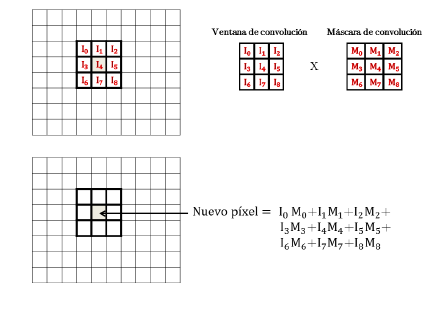
\includegraphics[width=0.7\linewidth]{Imagenes/convolucionsobreunaimagen}
	\caption{Operaci�n de convoluci�n sobre un pixel}
	\label{fig:convolucionsobreunaimagen}
\end{figure}

Las mascaras derivativas son utilizadas para calcular el gradiente de una imagen, normalmente con la intenci�n de detectar los contornos. Entre los m�s utilizados se encuentran: Sobel, Prewitt, Roberts y Laplaciano  \cite{Operadores}. En la Figura \ref{fig:derivadassobel} se muestra el efecto obtenido despu�s de aplicar el operador de Sobel en una imagen. 

\begin{figure}[H]
	\centering
	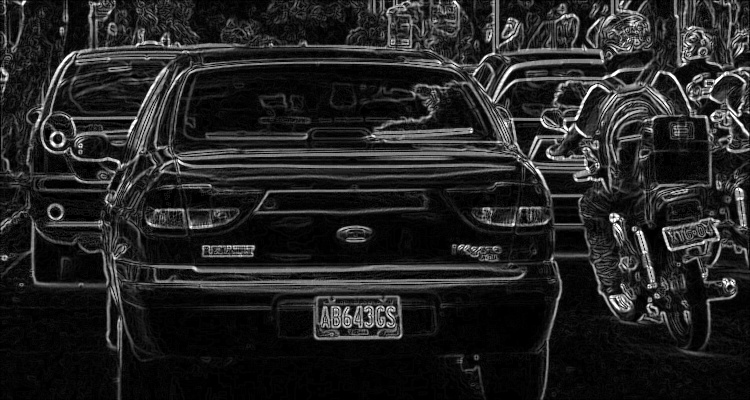
\includegraphics[width=0.7\linewidth]{Imagenes/Derivadas_Sobel}
	\caption{Operador Sobel}
	\label{fig:derivadassobel}
\end{figure}

Bibliotecas de software libre orientadas hacia la visi�n computarizada como OpenCv, ofrecen funciones que utilizan estos operadores para determinar el gradiente de la imagen y as� detectar los contornos mediante la umbralizaci�n como puede apreciarse en las Figuras \ref{fig:grisesvsadapt} y \ref{fig:sobelvsumbral}:

\begin{figure}[H]
	\centering
	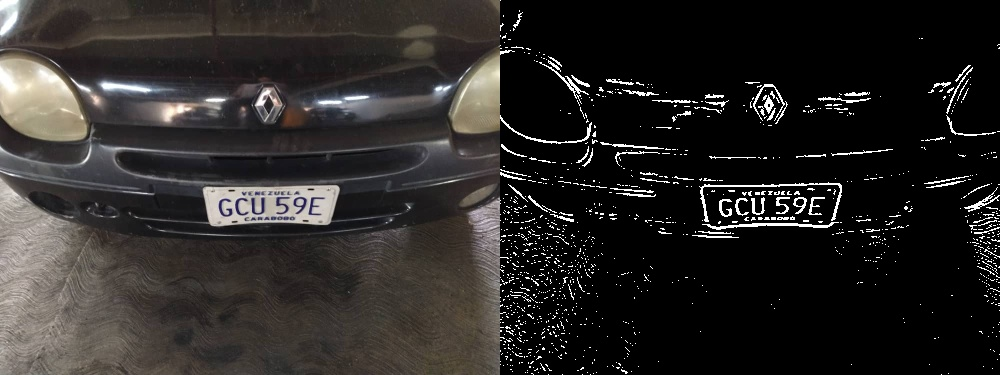
\includegraphics[width=0.7\linewidth]{Imagenes/grisesvsadapt}
	\caption{Umbralizaci�n adaptativa de librer�a OpenCV}
	\label{fig:grisesvsadapt}
\end{figure}

\begin{figure}[H]
	\centering
	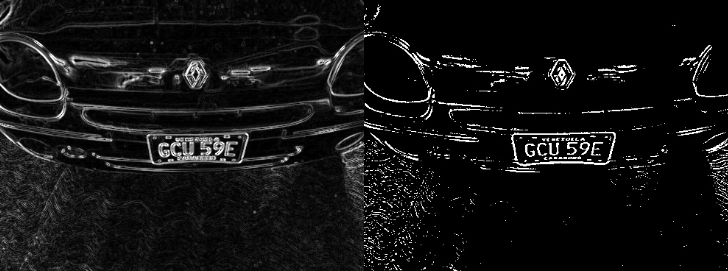
\includegraphics[width=0.7\linewidth]{Imagenes/sobelvsumbral}
	\caption{Filtro de sobel vs Umbralizaci�n adaptativa}
	\label{fig:sobelvsumbral}
\end{figure}

Existen otras funciones especializadas en la detecci�n de contornos como lo es Canny de OpenCV (Ver el ejemplo de la Figura \ref{fig:cannyvsumbral}).

\begin{figure}[H]
	\centering
	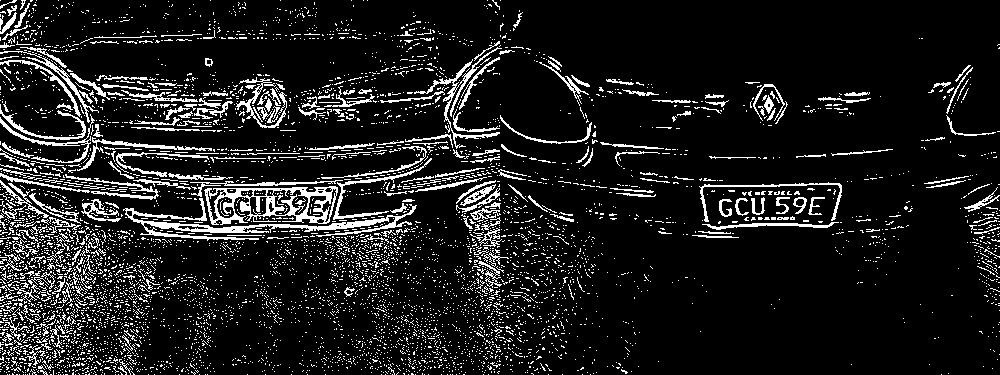
\includegraphics[width=0.7\linewidth]{Imagenes/cannyvsumbral}
	\caption{Funci�n Canny vs Umbralizaci�n adaptativa}
	\label{fig:cannyvsumbral}
\end{figure}




\subsection{Binarizaci�n}



La binarizaci�n es una t�cnica que consiste en la realizaci�n de un barrido en la matriz de la imagen digital, por medio de bucles o recursividad, con el fin de que el proceso produzca la reducci�n de la escala de grises a dos �nicos valores. Negro(= 0) y blanco (= 255), o lo que es lo mismo, un sistema binario de ausencia y presencia de color 0-1. La comparaci�n de cada p�xel de la imagen viene determinada por el umbral de
sensibilidad (valor T = Threshold). Por ejemplo, los valores que sean mayores que el umbral toman un valor 255 (blanco) y los menores 0 (negro). 

\begin{figure}[H]
	\centering
	
\includegraphics[width=0.5\linewidth]{Imagenes/umbralizacion}
	\caption{Imagen a color binarizada.}
	\label{fig:umbralizacion}
\end{figure}




En base a las particularidades entre algoritmos categorizan los m�todos de umbralizaci�n en seis grupos. Aqu� a�adimos uno m�s, los m�todos globales \cite{Binarizacion}:
\begin{itemize}
	
	\item \textit{Histograma}: m�todos basados en el an�lisis de los picos
	m�ximos y m�nimos de las curvas del histograma del suavizado de la imagen.
	
	\item \textit{Clustering}: m�todos basados en discernir como las muestras
	de los niveles de gris se agrupan o alternativamente se modelan como una mezcla de dos gaussianas.
	
	\item \textit{Entrop�a}: m�todos basados en el an�lisis de los resultados de
	la aplicaci�n de algoritmos que utilizan la entrop�a de las
	regiones frontal y de fondo, la entrop�a cruzada entre la imagen original y binarizada.
	
	\item \textit{Similitud}: m�todos basados en la b�squeda de una similitud
	entre las escalas de grises, como la tonalidad difusa, los bordes de la imagen, etc.
	
	\item \textit{Espaciales}: m�todos anal�ticos que usan el orden de distribuci�n, la probabilidad y/o la correlaci�n entre los diferentes
	p�xeles.
	
	\item \textit{Globales}: m�todos cuyo valor del umbral es est�tico.
	
	\item \textit{Locales}: m�todos que adaptan el valor del umbral, de forma
	manual o autom�tica, a cada p�xel dependiendo
	
\end{itemize}


\section{Machine Learning y M�quina de Soporte Vectorial}\label{CAP:ML}


``\textit{Machine Learning}'' (ML) o aprendizaje autom�tico (por su traducci�n al espa�ol) es una rama de la inteligencia artificial que est� constituida por un conjunto de algoritmos que automatizan la construcci�n de modelos anal�ticos a partir del an�lisis de datos. La ML se fundamenta en la idea de que los sistemas pueden aprender de los datos, identificar patrones y tomar decisiones con una m�nima intervenci�n humana. La ML tambi�n se puede definir como el proceso de resolver un problema pr�ctico mediante (\cite{SarkarBaliSharma:2018}): 1)~la recopilaci�n de un conjunto de datos y 2) la construcci�n algor�tmica de un modelo estad�stico basado en ese conjunto de datos.

Por lo general, los m�todos de aprendizaje autom�tico se pueden clasificar de m�ltiples maneras bajo m�ltiples paradigmas. En el presente trabajo utilizamos la clasificaci�n basada en la cantidad de supervisi�n humana en el proceso de aprendizaje, a saber:
\begin{enumerate}[\indent a.]
   \item \textit{Aprendizaje supervisado}
  \item \textit{Aprendizaje no supervisado}
  \item \textit{Aprendizaje semi-supervisado}
  \item \textit{Aprendizaje reforzado}
\end{enumerate}

\subsubsection{Aprendizaje Supervisado}

Los m�todos o algoritmos de aprendizaje supervisado incluyen algoritmos de aprendizaje que toman muestras de datos (conocidas como datos de entrenamiento) y salidas asociadas (conocidas como etiquetas o respuestas) con cada muestra de datos durante el proceso de entrenamiento del modelo. El objetivo principal es aprender un mapeo o asociaci�n entre las muestras de datos de entrada $x$ y sus correspondientes salidas $y$, bas�ndose en m�ltiples instancias de datos de entrenamiento. Este conocimiento aprendido se puede utilizar en el futuro para predecir una salida $y'$ para cualquier nueva muestra de datos de entrada $x'$, que antes se desconoc�a o no se ve�a durante el proceso de entrenamiento del modelo. Estos m�todos se denominan supervisados porque el modelo aprende sobre muestras de datos donde las respuestas/etiquetas de salida deseadas ya se conocen de antemano en la fase de entrenamiento (\cite{SarkarBaliSharma:2018}).

Existen dos clases principales de m�todos de aprendizaje supervisado, seg�n el tipo de tareas de aprendizaje autom�tico que pretenden resolver:
\begin{itemize}
  \item Regresi�n
  \item Clasificaci�n
\end{itemize}

El objetivo principal de los m�todos de aprendizaje supervisado para regresi�n es la estimaci�n de un valor. Los m�todos para regresi�n se entrenan en muestras de datos de entrada que tienen respuestas de salida que son valores num�ricos continuos. Los modelos de regresi�n hacen uso de atributos o caracter�sticas de los datos de entrada (tambi�n llamados variables explicativas o independientes) y sus correspondientes valores num�ricos continuos de salida (tambi�n llamados respuesta, dependiente o variable de resultado) para aprender relaciones y asociaciones espec�ficas entre las entradas y sus salidas correspondientes. Con este conocimiento, se puede predecir la respuesta de salida para instancias de datos nuevas y no vistas similares a la clasificaci�n pero con salidas num�ricas continuas.

En cambio, el objetivo principal de los m�todos de aprendizaje supervisado para clasificaci�n es predecir etiquetas de salida o respuestas que son de naturaleza categ�rica para los datos de entrada en funci�n de lo que el modelo ha aprendido en la fase de entrenamiento. Las etiquetas de salida aqu� tambi�n se conocen como clases o etiquetas de clase, ya que son de naturaleza categ�rica, lo que significa que son valores discretos y desordenados. Por lo tanto, cada respuesta de salida pertenece a una categor�a o clase discreta espec�fica. Un m�todo de aprendizaje supervisado para clasificaci�n es la \textit{M�quina de Soporte Vectorial} (SVM, por sus siglas en ingl�s: Support Vector Machine) el cual describiremos m�s adelante.


\subsubsection{Aprendizaje No Supervisado}

Los m�todos de aprendizaje no supervisado extraen conocimientos o informaci�n significativa de los datos en lugar de intentar predecir alg�n resultado basado en datos de entrenamiento supervisado previamente disponibles. Hay m�s incertidumbre en los resultados del aprendizaje no supervisado, pero tambi�n puede obtener mucha informaci�n de estos modelos que antes no estaba disponible para ver con solo mirar los datos sin procesar. A menudo, el aprendizaje sin supervisi�n podr�a ser una de las tareas involucradas en la construcci�n de un enorme sistema de inteligencia (\cite{SarkarBaliSharma:2018}). Los m�todos de aprendizaje no supervisado se pueden clasificar en las siguientes �reas de la ML de mucha importancia para el aprendizaje no supervisado:
\begin{itemize}
  \item Agrupaci�n
  \item Reducci�n de dimensionalidad
  \item Detecci�n de anomal�as
  \item Asociaci�n de miner�a de reglas
\end{itemize}

\subsubsection{Aprendizaje Semi-Supervisado}

Los m�todos de aprendizaje semi-supervisados generalmente se encuentran entre los m�todos de aprendizaje supervisados y no supervisados. Estos m�todos suelen utilizar una gran cantidad de datos de entrenamiento que no est�n etiquetados (que forman el componente de aprendizaje no supervisado) y una peque�a cantidad de datos previamente etiquetados y anotados (que forman el componente de aprendizaje supervisado). Hay m�ltiples t�cnicas disponibles en forma de m�todos generativos, m�todos basados en gr�ficos y m�todos basados en heur�stica. (\cite{SarkarBaliSharma:2018})

\subsubsection{Aprendizaje Reforzado}

Los m�todos de aprendizaje reforzado son un poco diferentes de los m�todos convencionales supervisados o no supervisados. En este contexto, se cuenta con un agente que se desea capacitar durante un per�odo de tiempo para interactuar con un entorno espec�fico y mejorar su desempe�o durante un per�odo de tiempo, con respecto al tipo de acciones que realiza sobre el entorno. Normalmente, el agente comienza con un conjunto de estrategias o pol�ticas para interactuar con el entorno. Al observar el medio ambiente, toma una acci�n particular basada en una regla o pol�tica y observando el estado actual del medio ambiente. Seg�n la acci�n, el agente obtiene una recompensa, que podr�a ser beneficiosa o perjudicial en forma de penalizaci�n. Actualiza sus pol�ticas y estrategias actuales si es necesario y este proceso iterativo contin�a hasta que aprende lo suficiente sobre su entorno para obtener las recompensas deseadas. Los pasos principales de un m�todo de aprendizaje por refuerzo se mencionan a continuaci�n. (\cite{SarkarBaliSharma:2018})
\begin{enumerate}[\indent 1.]
  \item Prepare al agente con un conjunto de pol�ticas y estrategias iniciales.
  \item Observe el entorno y el estado actual.
  \item Seleccione la pol�tica �ptima y realice una acci�n.
  \item Obtenga la recompensa (o penalizaci�n) correspondiente.
  \item Actualice las pol�ticas si es necesario.
  \item Repita los pasos 2 a 5 de forma iterativa hasta que el agente aprenda las pol�ticas m�s �ptimas.
\end{enumerate}



\subsection{M�quina de Soporte Vectorial}

La SVM es un algoritmo de aprendizaje supervisado normalmente empleado en problemas de clasificaci�n y, recientemente, en problemas de regresi�n. Los fundamentos matem�ticos de la SVM han sido desarrollados por Vapnik~\cite{Vapnik:1995} y est�n ganando popularidad debido a muchas caracter�sticas atractivas y un rendimiento emp�rico prometedor. 

El problema de clasificaci�n puede restringirse a la consideraci�n del problema de dos clases sin p�rdida de generalidad. Muchos problemas de clasificaci�n pueden ser resueltos por la SVM si los grupos son linealmente separables. En este problema, el prop�sito es separar las dos clases mediante una funci�n que se induce a partir de los datos disponibles. El objetivo principal es producir un clasificador que funcione bien en ejemplos invisibles, es decir, que generalice bien. Considere el ejemplo de la Figura~\ref{fig:hiperplano}. Aqu� hay muchos clasificadores lineales posibles que pueden separar los datos, pero solo hay uno que maximiza la distancia entre �l y el conjunto de datos m�s cercano de cada clase. Este clasificador lineal se denomina \textit{hiperplano de separaci�n �ptimo}. Intuitivamente, esperar�amos que este l�mite se generalizara bien en oposici�n a los otros l�mites posibles. 

\begin{figure}[!h]
\centering
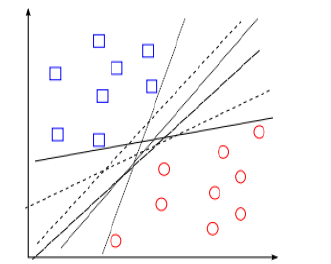
\includegraphics[width=0.32\linewidth]{Imagenes/varios_hiperplanos}
\caption{Hiperplanos de separaci�n.}
\label{fig:hiperplano}
\end{figure}

En caso que los datos no sean linealmente separables, existen procedimientos que emplean funciones denominadas \textit{n�cleos}, las cuales permiten usar la SVM para la separaci�n de las clases. Pasemos a dar una breve descripci�n matem�tica de la SVM.

\subsubsection{Datos Linealmente Separables}

Asumamos que los datos a clasificar pueden ser separados linealmente en dos clases,
\[
(\x_{1},y_{1}),(\x_{2},y_{2}),\ldots,(\x_{p},y_{p}),\quad\x\in\R^{n},\quad y_{i}\in\{-1,+1\},
\]
donde el $(\x_{i},y_{i})$ es un dato de entrenamiento, con $\x_{i}$ el \textit{vector de atributos} e $y_{i}$ la \textit{etiqueta}. Se desea encontrar una funci�n $f:\R^{n}\to\{-1,+1\}$, denominada \textit{funci�n de clasificaci�n}, que separe los dos clases de datos, es decir,
\[
f(\x_{i}) = y_{i},\quad i=1,2,\ldots,p.
\]
Ahora bien, como los datos son linealmente separables, existen $\w\in\R^{n}$ y $b\in\R$ tales que el hiperplano 
\[
\{\x\in\R^{n}:\w^{\top}\x+b = 0\}
\]
separa las dos clases, esto es, los datos de clases opuestas est�n en lados opuestos del
hiperplano. 

\begin{figure}[!h]
\centering
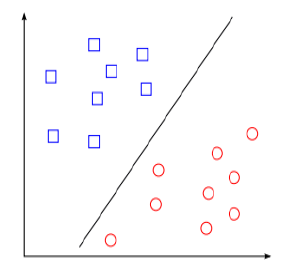
\includegraphics[width=0.32\linewidth]{Imagenes/hiperplano}
\caption{Datos e hiperplano $\w^{\top}\x+b = 0$}
\label{fig:hiperplan}
\end{figure}

El hiperplano de la Figura~\ref{fig:hiperplan} se construye a partir de los datos $\x_{i}$ y de sus etiquetas $y_{i}$. En este caso, la funci�n $f(\x)$ puede ser expresada como:
\[
f(\x) = \sgn(\w^{\top}\x+b),
\]
donde $\sgn(\cdot)$ es la funci�n signo. De esta forma, el problema se reduce a encontrar $\w\in\R^{n}$ (\textit{vector de pesos} que ajusta el modelo), y un escalar $b$ (conocido como sesgo) tales que
\[
y_{i}(\w^{\top}\x+b) > 0,\qquad \mbox{para }i=1,2,\ldots,p.
\]
Pero, existen infinitos hiperplanos que satisfacen esta condici�n (ver Figura~\ref{fig:hiperplano}). 

\begin{figure}[!h]
\centering
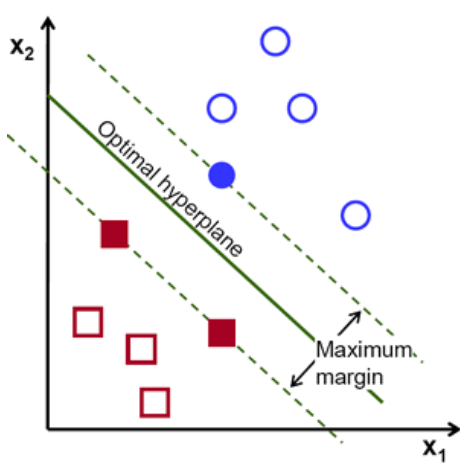
\includegraphics[width=0.32\linewidth]{Imagenes/maximomargen}
\caption{Hiperplano de separaci�n �ptimo. M�ximo margen de separaci�n.}
\label{fig:maximomargen}
\end{figure}

El problema anterior se resuelve determinando el hiperplano de separaci�n �ptimo. Este hiperplano es aquel cuyo margen de separaci�n entre los vectores de dos clases es m�ximo. La propiedad fundamental del hiperplano de separaci�n �ptimo es que este equidista del dato m�s cercano de cada clase \cite{SVN} (ver Figura~\ref{fig:maximomargen}). En otras palabras, para determinar el hiperplano de separaci�n �ptimo se debe resolver el siguiente problema de optimizaci�n con restricciones:
\begin{equation}\label{posvm1}
\begin{split}
\max\limits_{\w,b,\|\w\|=1} & \quad M\\
\mbox{sujeto a:} & \quad y_{i}(\w^{\top}\x_{i}+b) \geq M,\qquad\mbox{para }i=1,2,\ldots,p,
\end{split}
\end{equation}
donde $M$ es la distancia del hiperplano a cada lado. El margen m�ximo que se muestra en la Figura~\ref{fig:maximomargen} tiene $2M$ unidades de ancho. Sin  p�rdida de generalidad, podemos suponer que $\|\w\|=1/M$. Por lo que el problema \eqref{posvm1} es equivalente a:
\begin{equation}\label{posvm2}
\begin{split}
\min\limits_{\w,b} & \quad\frac{1}{2}\|\w\|^{2}\\
\mbox{sujeto a:} & \quad y_{i}(\w^{\top}\x_{i}+b) \geq 1,\qquad\mbox{para }i=1,2,\ldots,p.
\end{split}
\end{equation}
El problema \eqref{posvm2} se puede expresar en forma matricial como:
\begin{equation}\label{posvm3}
\begin{split}
\min\limits_{\w,b} & \quad\frac{1}{2}\w^{\top}\w\\
\mbox{sujeto a:} & \quad AX^{\top}\w + b\y \geq \uno,
\end{split}
\end{equation}
donde $A=\mathrm{diag}(y_{1},y_{2},\ldots,y_{p})\in\R^{p\times p}$ es una matriz diagonal, $\y=(y_{1},y_{2},\ldots,y_{p})^{\top}\in\R^{p}$ es el \textit{vector de etiquetas}, $\uno\in\R^{p}$ es el vector de unos, y $X=\begin{pmatrix}\x_{1} & \x_{2} & \cdots & \x_{p}\end{pmatrix}\in\R^{n\times p}$ es la matriz de atributos, cuyas columnas son 
los datos $\x_{i}$.

Utilizando los multiplicadores de Lagrange, el problema \eqref{posvm3} puede expresarse en la siguiente forma, denominada \textit{problema dual de Wolfe},
\begin{equation}\label{posvm4}
\begin{split}
\min\limits_{\vmu} & \quad\frac{1}{2}\vmu^{\top}Q\vmu - \vmu^{\top}\uno \\
\mbox{sujeto a:} & \quad \vmu^{\top}\y = 0,\\
& \quad\vmu \geq 0.
\end{split}
\end{equation}
donde $Q=AX^{\top}XA$, $\vmu=(\mu_{1},\ldots,\mu_{p})^{\top}\in\R^{p}$, y $\mu_{i}$ son los multiplicadores de Lagrange. El problema dual de Wolfe puede resolverse eficientemente, ya que es un problema cuadr�tico y existen en la literatura algoritmos eficientes para la optimizaci�n cuadr�tica.

De todo lo anterior, para obtener la funci�n $f(\x) = \sgn(\x^{\top}\w^{*}+b^{*})$ que separe los $p$ pares $(\x_{1},y_{1}),(\x_{2},y_{2}),\ldots,(\x_{p},y_{p})$ de datos etiquetados, se debe realizar el siguiente procedimiento, que hemos denominados Procedimiento de Separaci�n:

\bigskip

\textbf{Procedimiento de Separaci�n}
\begin{enumerate}[\indent\bf1.]
  \item Resolver el problema \eqref{posvm4} para obtener los multiplicadores de Lagrange $\vmu^{*}$.

  \item Calcular el vector $\w^{*}$ por:
    \[
    \w^{*} = XA\boldsymbol{\vmu}^{*} = \sum_{i=1}^{p}\mu_{i}^{*}y_{i}\x_{i}.
    \]

  \item Calcular $b$ utilizando la ecuaci�n:
    \[
    b^{*} = y_{i_{max}}-\x_{i_{max}}^{\top}\w^{*},
    \]
    donde $i_{max}=\argmax\limits_{i=1,2,\ldots,p}\{\mu_{i}\}$.
\end{enumerate}

Los \textbf{vectores de soporte} son los datos $\x_{i}$ tales que sus multiplicadores de Lagrange $\mu_{i}^{*}$ son positivos. Generalmente los vectores de soporte representan una peque�a porci�n de todos los datos de entrenamiento y son aquellos datos que se encuentran m�s cercanos al hiperplano de separaci�n �ptimo. La mayor�a de los algoritmos para resolver el problema \eqref{posvm4}, tienen como estrategia identificar los vectores de soporte para reducir el tama�o del problema durante el entrenamiento. Todo este procedimiento de c�lculo est� implementado de manera eficiente en algunas librer�as de Python, en especial en la librer�a \textbf{Scikit-Learn}, de la cual hablaremos m�s adelante.


\subsubsection{Datos No Linealmente Separables}

Cuando los datos $\x_{i}$ no son linealmente separables, existe una funci�n no lineal
$\phi:\R^{n}\to\R^{n}$ tal que los datos definidos como
\[
\z_{i} = \phi(\x_{i}),\quad i=1,2,\ldots,p
\]
son linealmente separables \cite{Cover:1965}. Usando este hecho se puede encontrar un separador no lineal para los datos $\x_{i}$ con SVM aplicando la misma t�cnica usada en el caso del separador lineal, pero con los datos $\z_{i}$. En este caso, la funci�n de clasificaci�n viene dada por:
\[
f(\x) = \sgn(\phi(\x)^{\top}\w^{*} + b^{*}),
\]
donde $\w^{*}$ y $b^{*}$ se obtienen resolviendo el problema \eqref{posvm4} y aplicando el Procedimiento de Separaci�n, tomando $\z_{1},\z_{2},\ldots,\z_{p}$ como datos de entrenamiento. La funci�n $\phi$, en general, no se conoce expl�citamente, adem�s, es poco pr�ctico calcularla. En la pr�ctica, se usan las funciones llamadas \textit{n�cleo}, $\mathcal{K}:\R^{n}\times\R^{n}\to\R$, tales que
\[
\mathcal{K}(\x,\z) = \phi(\x)^{\top}\phi(\z),\qquad\mbox{para }\x,\z\in\R^{n}.
\]
Con un n�cleo $\mathcal{K}$ dado, se construye la matriz $Q=(q_{ij})$ del problema \eqref{posvm4} como:
\[
q_{ij} = y_{i}y_{j}\mathcal{K}(\x_{i},\x_{j}),\qquad\mbox{para }i,j=1,2,\ldots,p.
\]
Por lo que, la funci�n de clasificaci�n en el caso no separable linealmente, es:
\[
f(\x) = \sgn(\sum_{i=1}^{p}y_{i}\mu_{i}^{*}\mathcal{K}(\x,\x_{i})+b^{*}),
\]
donde
\[
b^{*} = y_{j}-\sum_{i=1}^{p}y_{i}\mu_{i}^{*}\mathcal{K}(\x_{j},\x_{i}),\qquad
\mbox{para alg�n $j$ tal que }\mu_{j}^{*}>0.
\]

No toda funci�n $\mathcal{K}$ es un n�cleo. La funciones n�cleo deben ser sim�tricas, esto es $\mathcal{K}(\x,\z) = \mathcal{K}(\z,\y)$, adem�s, la matriz $K=(k_{ij})$ definida como $k_{ij}=\mathcal{K}(\x_{i},\x_{j})$ debe ser sim�trica semidefinida positiva\footnote{Una matriz $A\in\R^{n\times n}$ es sim�trica semidefinida positiva si $A^{\top}=A$ y $\x^{\top}A\x \geq0$, para todo $\x\in\R^{n}$.}. A continuaci�n se listan las funciones n�cleos m�s usadas en las aplicaciones.

\begin{enumerate}[\indent1.]
  \item \textit{Lineal}: $\mathcal{K}(\x,\z) = \x^{\top}\z$
  
  \item \textit{Polinomio de grado $d$}: $\mathcal{K}(\x,\z) = (\gamma\x^{\top}\z + r)$, con par�metros $\gamma,r\in\R$.
      
  \item \textit{Base radial (RBF)}: $\mathcal{K}(\x,\z) = e^{-\gamma\|\x-\z\|^{2}}$, con par�metro $\gamma\ in \R$.
      
  \item \textit{Red neuronal (Sigmoid)}: $\mathcal{K}(\x,\z) = \tanh(\gamma\x^{\top}\z + r)$, con par�metros $\gamma,r\in\R$.
\end{enumerate}

El procedimiento de separaci�n cuando los datos son no linealmente separables, adem�s del caso cuando hay multiples clases, tambi�n est� implementado en la librer�a \textbf{Scikit-Learn}.

En resumen, el objetivo de la SVM es idear un m�todo de aprendizaje computacionalmente eficiente. Los hiperplanos optimizan el l�mite de generalizaci�n, por lo tanto el algoritmo es capaz de manejar grandes dimensiones (\cite{SVM2014}). Algunas de las ventajas de las SVMs frente a otros algoritmos son las siguientes (\cite{Sklearn}):

\begin{itemize}
\item Efectividad en espacios de grandes dimensiones.
	
\item Sigue siendo efectivo incluso en casos donde el n�mero de dimensiones es m�s grande que el n�mero de ejemplos de entrenamiento.
	
\item Usa un subconjuto de los datos de entrenamiento en la funci�n de decisi�n (los vectores de soporte), por lo tanto es eficiente computacionalmente, en especial en el uso de la memoria.
	
\item Es vers�til: diferentes funciones n�cleo pueden emplearse para definir funci�n de clasificaci�n. Los n�cleos comunes son f�ciles de personalizar.
\end{itemize}



\section{Lenguaje de programaci�n Python}

Python es un lenguaje de programaci�n multiparadigma, multiplataforma, din�mico e interpretado, es decir, se ejecuta directamente mediante un int�rprete dejando a un lado la compilaci�n. Actualmente, Python es  administrado por Python Software Foundation. El software posee una licencia de c�digo abierto denominada Python Software Fondation License.


Python se caracteriza por su amplia aplicabilidad en diferentes campos del desarrollo de nuevas tecnolog�as como: Machine Learning, Data Science, Vision por Computador, entre otros. Python soporta diferentes librer�as como  OpenCV  y Scikit-Learn, las cuales cuentan con extensa documentaci�n acerca de sus aplicaciones e implementaciones. La versi�n que se utiliz� para la implementaci�n de este trabajo fue Python 3.1.

\section{OpenCV}

Open Computer Vision (OpenCV, por sus sigl�s en ingl�s) es una librer�a libre de visi�n artificial desarrollada originalmente por Intel. Especializada en la visi�n por computador y el procesamiento de im�genes cuenta con diferentes herramientas que permiten manipular la informaci�n dentro de una imagen. Para mayor informaci�n visitar  https://opencv.org/. La versi�n que se utiliz� para la implementaci�n de este trabajo fue OpenCV 3.4.


Espec�ficamente, las funciones de OpenCV empleadas en la implementaci�n son:

\begin{itemize}
	
	\item \verb|cv2.imread|: permite llamar una imagen digital al ambiente de desarrollo empleado para as� poder manipularla mediante todas las otras herramientas que ofrece la librer�a. \cite{imread}
	
	
	\item \verb|img.shape|: lee y devuelve las dimensiones de una imagen digital en funci�n del ancho y alto. \cite{imgshape}
	
	\item \verb|cv2.resize|: redimensiona el ancho y alto de una imagen de acuerdo a los par�metros de entrada especificados.  \cite{resize}
	
	\item \verb|cv2.GaussianBlur|: es un filtro que suaviza la definici�n de la imagen a trav�s de un kernel Gaussiano. El filtrado gaussiano se realiza convolucionando cada punto de la matriz de entrada con un n�cleo gaussiano y luego sum�ndolos a todos para producir la matriz de salida. \cite{GaussianBlur}
	
	\item \verb|cv2.cvtColor|: cambia el espacio de color de una imagen digital 
	a otro. \cite{cvTcolor}
	
	\item \verb|cv2.adaptiveThreshold|: el m�todo adaptativetreshold binariza una imagen de acuerdo a un valor de umbral que c�lcula para peque�as regiones de la imagen digital. As�, el filtro gaussiano realiza una convoluci�n con cada punto de la matriz generando una matriz de salida. El valor de umbral es calculado como la suma ponderada de los valores del vecindario donde los pesos son una ventana gaussiana. Las dimesiones del kernel representa el tama�o del vecindario de pixeles usados para calcular el valor umbral. \cite{AdaptTresh}
	
	\item \verb|cv2.dilate|: Dilate es un m�todo de transformaci�n morfol�gica. Las operaciones morfol�gicas aplican un elemento estructurante a la imagen de entrada y generan una de salida con caracter�sticas morfol�gicas diferentes. Dilate utiliza un kernel \textit{B} el cual se escanea sobre la imagen, calcula el valor m�ximo de pixeles superpuestos por \textit{B}  y reemplazamos el p�xel de la imagen en la posici�n del punto de anclaje con ese valor m�ximo. Como se puede deducir, esta operaci�n de maximizaci�n hace que las regiones brillantes dentro de una imagen `` crezcan". \cite{Dilate}
	
	\item \verb|cv2.findcontours|: definiendo contorno como una curva donde todos los puntos continuos  tienen el mismo color o intensidad, este m�todo encuentra los contornos definidos en una imagen, preferiblemente binarizada. Este m�todo requiere diferentes par�metros de entrada que definen su modo de funcionamiento como le modo de recuperaci�n de contorno y m�todo de aproximaci�n de contorno. Ambos par�metros son explicados en las fuentes de documentaci�n. \cite{findContours}
	
	\item \verb|cv2.boundingRect|: esta funci�n calcula y devuelve el rect�ngulo delimitador de un contorno o un conjunto de p�xeles de la misma intensidad y distintos de cero. Esta funci�n c�lcula un rectangulo recto, es decir, no considera �ngulo de rotaci�n por lo tanto el �rea del rect�ngulo no ser� m�nima. Esta funci�n devuelve las coordenadas de la esquina superior izquierda del rect�ngulo, su ancho y alto. \cite{boundRectangle}
	
	\item \verb|cv2.rectangle|: esta funci�n es una de las funciones de dibujo de la librer�a \textit{OpenCV} y dibuja un rect�ngulo en la imagen, dadas unas coordenadas espec�ficas, con color y ancho de l�nea espec�fico. La funci�n devuelve la imagen con dicho pol�gono dibujado. \cite{rectangle}
	
\end{itemize} 	

\section{Scikit-Learn}

Scikit-Learn por su parte, es una biblioteca con basto desarrollo en el aprendizaje autom�tico, de software libre para el lenguaje de programaci�n Python. Cuenta con varios algoritmos de regresi�n, clasificaci�n y an�lisis de grupos como SVMs, Clustering, K-means, entre otros. Esta biblioteca inici� como un proyecto de Google Summer of code por David Cournapeau en el 2007. Para mayor informaci�n y detalles acerca de la biblioteca dirigirse a http://scikit-learn.org/stable/.  



%

%==================================================================
\chapter{MARCO METODOL�GICO}\label{CAP:met}
%\markboth{Tu Primer Cap?tulo}{Tu Primer Cap?tulo}%
% !TeX encoding = ISO-8859-1
% !TeX spellcheck = es_ES

\section{Tipo de investigaci�n}

Considerando el problema, referido al dise�o de un sistema de reconocimiento de matr�culas vehiculares, la modalidad de investigaci�n del presente proyecto es \textit{Proyecto factible} de acuerdo el Manual de la UPEL. Adicionalmente, el dise�o podr� ser integrado a prototipos de sistemas de vigilancia veh�cular. ``El Proyecto Factible consiste en la investigaci�n, elaboraci�n y desarrollo de una propuesta de un modelo operativo viable para solucionar  problemas, requerimientos o necesidades de organizaciones o grupos sociales; puede referirse a la formulaci�n de pol�ticas, programas, tecnolog�as, m�todos o procesos. El Proyecto debe tener apoyo en una investigaci�n de tipo documental, de campo o un dise�o que incluya ambas modalidades."  \cite{Manual}

\section{Fases metodol�gicas}

A continuaci�n, se presentan las fases que se llevaron a cabo para el desarrollo del trabajo de grado:

\subsection{Recopilaci�n de informaci�n}

Se llev� a cabo una investigaci�n documental acerca de: 
\begin{itemize}
	
	\item Procesamiento de im�genes.
	
	\begin{itemize}
		\item Imagen digital.
		
		\item Espacios de color.
		
		\item Mascaras derivativas discretas.
		
		\item Binarizaci�n. 
		
	
		
	\end{itemize}	
	
	
	
	\item Lenguaje de programaci�n Python. 
	
	\item OpenCV para procesamiento de im�gen.
	
	\item M�quina de Soporte Vectorial.
	
\end{itemize}

Tomando en cuenta el estado del arte en procesamiento de im�genes con referencias t�cnicas apropiadas de la informaci�n disponible en la red.


\subsection{Selecci�n}


 Con base a la informaci�n obtenida, se seleccionaron las t�cnicas de procesamiento de imagen m�s adecuadas a las necesidades de la detecci�n de la placa y segmentaci�n de los caracteres. La selecci�n se caracteriz� por  obtener t�cnicas que hayan sido probadas y optimizadas en diferentes experimentos, de c�digo abierto y con la informaci�n necesaria para la compresi�n de sus conceptos. Se seleccion� la librer�a de c�digo abierto OpenCV,  debido a su amplia utilizaci�n  en la visi�n por computador y procesamientos de im�genes. OpenCV es una librer�a con gran variedad de t�cnicas y aplicaciones, siendo una herramienta empleada en diversos entornos e incluso en investigaciones recientes en el campo de la visi�n por computador. Tomando en cuenta lo anterior, se profundiz� en las t�cnicas que permitir�an el filtrado de la informaci�n de inter�s en una imagen de condiciones controladas. Por otro lado, se seleccion� la M�quina de Soporte Vectorial, siendo uno  de los algoritmos m�s eficientes e importantes en el mundo del machine learning. Dada su capacidad y efectividad, es un algoritmo que ha participado en diferentes campos de desarrollo, entre los cuales tambi�n se encuentra la visi�n por computador. Considerando lo anterior, se decidi� explorar su potencialidad en la clasificaci�n de caracteres.

	
\subsection{Evaluaci�n de aplicabilidad}

 Con el fin de evaluar la factibilidad se dise�� un diagrama de flujo a fin de definir las instrucciones generales necesarias para lograr el procesamiento de imagen con los resultados deseados. Se realizaron pruebas preliminares para evaluar los resultados experimentales obtenidos con los esperados y as� determinar su factibilidad. 
 
 
 \subsection{Programaci�n y dise�o}
 
 Una vez seleccionadas las t�cnicas para el procesamiento de im�genes y el algoritmo para la clasificaci�n y reconocimiento de patrones, se procedi� a dise�ar de manera modular la estructura del programa. En funci�n de lo anterior, a partir del diagrama de flujo obtenido, se elabor� el pseudoc�digo y, de esta manera, se describieron las funciones de cada una de las etapas que componen el proyecto. 
 
   
 \subsection{Implementaci�n y pruebas}
 
 Por �ltimo, se procedi� a implementar de manera modular toda la l�gica necesaria para cada una de las etapas descritas en el pseudoc�digo en el lenguaje Python. Se realizaron experiencias computacionales orientadas a la verificaci�n del sistema de reconocimiento de matr�culas. En primera instancia, se dise�aron pruebas dirigidas a monitorear el desempe�o y la funcionalidad del programa, donde se tomaron acciones a fin de ajustar el algoritmo para obtener los resultados esperados.
  %

%==================================================================
%\chapter{DEFINICI�N Y DESCRIPCI�N DEL HARDWARE}\label{CAP:hard}
%\markboth{Tu Segundo Cap?tulo}{Tu Segundo Cap?tulo}%
%% !TeX encoding = ISO-8859-1
% !TeX spellcheck = es_ES

\section{Tipo de investigaci�n}

Considerando el problema, referido al dise�o de un sistema de reconocimiento de matr�culas vehiculares, la modalidad de investigaci�n del presente proyecto es \textit{Proyecto factible} de acuerdo el Manual de la UPEL. Adicionalmente, el dise�o podr� ser integrado a prototipos de sistemas de vigilancia veh�cular. ``El Proyecto Factible consiste en la investigaci�n, elaboraci�n y desarrollo de una propuesta de un modelo operativo viable para solucionar  problemas, requerimientos o necesidades de organizaciones o grupos sociales; puede referirse a la formulaci�n de pol�ticas, programas, tecnolog�as, m�todos o procesos. El Proyecto debe tener apoyo en una investigaci�n de tipo documental, de campo o un dise�o que incluya ambas modalidades."  \cite{Manual}

\section{Fases metodol�gicas}

A continuaci�n, se presentan las fases que se llevaron a cabo para el desarrollo del trabajo de grado:

\subsection{Recopilaci�n de informaci�n}

Se llev� a cabo una investigaci�n documental acerca de: 
\begin{itemize}
	
	\item Procesamiento de im�genes.
	
	\begin{itemize}
		\item Imagen digital.
		
		\item Espacios de color.
		
		\item Mascaras derivativas discretas.
		
		\item Binarizaci�n. 
		
	
		
	\end{itemize}	
	
	
	
	\item Lenguaje de programaci�n Python. 
	
	\item OpenCV para procesamiento de im�gen.
	
	\item M�quina de Soporte Vectorial.
	
\end{itemize}

Tomando en cuenta el estado del arte en procesamiento de im�genes con referencias t�cnicas apropiadas de la informaci�n disponible en la red.


\subsection{Selecci�n}


 Con base a la informaci�n obtenida, se seleccionaron las t�cnicas de procesamiento de imagen m�s adecuadas a las necesidades de la detecci�n de la placa y segmentaci�n de los caracteres. La selecci�n se caracteriz� por  obtener t�cnicas que hayan sido probadas y optimizadas en diferentes experimentos, de c�digo abierto y con la informaci�n necesaria para la compresi�n de sus conceptos. Se seleccion� la librer�a de c�digo abierto OpenCV,  debido a su amplia utilizaci�n  en la visi�n por computador y procesamientos de im�genes. OpenCV es una librer�a con gran variedad de t�cnicas y aplicaciones, siendo una herramienta empleada en diversos entornos e incluso en investigaciones recientes en el campo de la visi�n por computador. Tomando en cuenta lo anterior, se profundiz� en las t�cnicas que permitir�an el filtrado de la informaci�n de inter�s en una imagen de condiciones controladas. Por otro lado, se seleccion� la M�quina de Soporte Vectorial, siendo uno  de los algoritmos m�s eficientes e importantes en el mundo del machine learning. Dada su capacidad y efectividad, es un algoritmo que ha participado en diferentes campos de desarrollo, entre los cuales tambi�n se encuentra la visi�n por computador. Considerando lo anterior, se decidi� explorar su potencialidad en la clasificaci�n de caracteres.

	
\subsection{Evaluaci�n de aplicabilidad}

 Con el fin de evaluar la factibilidad se dise�� un diagrama de flujo a fin de definir las instrucciones generales necesarias para lograr el procesamiento de imagen con los resultados deseados. Se realizaron pruebas preliminares para evaluar los resultados experimentales obtenidos con los esperados y as� determinar su factibilidad. 
 
 
 \subsection{Programaci�n y dise�o}
 
 Una vez seleccionadas las t�cnicas para el procesamiento de im�genes y el algoritmo para la clasificaci�n y reconocimiento de patrones, se procedi� a dise�ar de manera modular la estructura del programa. En funci�n de lo anterior, a partir del diagrama de flujo obtenido, se elabor� el pseudoc�digo y, de esta manera, se describieron las funciones de cada una de las etapas que componen el proyecto. 
 
   
 \subsection{Implementaci�n y pruebas}
 
 Por �ltimo, se procedi� a implementar de manera modular toda la l�gica necesaria para cada una de las etapas descritas en el pseudoc�digo en el lenguaje Python. Se realizaron experiencias computacionales orientadas a la verificaci�n del sistema de reconocimiento de matr�culas. En primera instancia, se dise�aron pruebas dirigidas a monitorear el desempe�o y la funcionalidad del programa, donde se tomaron acciones a fin de ajustar el algoritmo para obtener los resultados esperados.
  %

%==================================================================
\chapter{DEFINICI�N Y DESCRIPCI�N DEL SOFTWARE}\label{CAP:soft}
%\markboth{Tu Segundo Cap?tulo}{Tu Segundo Cap?tulo}%
% !TeX spellcheck = es_ES
% !TeX encoding = ISO-8859-1


En el presente cap�tulo se describe el proceso de desarrollo del proyecto, donde se detallan los procedimientos llevados a cabo a fin de cumplir los objetivos planteados.


\section{Arquitectura de software}

El software se bas� en una arquitectura estructural. Para cumplir la condici�n anterior, dado el problema que se desea resolver a trav�s de un algoritmo, se divide dicho algoritmo en m�dulos siguiendo los principio de dise�o de descomposici�n por refinamiento sucesivo, creaci�n de jerarqu�a modular y elaboraci�n de m�dulos independientes.

Los procesos descritos fueron dise�ados para trabajar de forma modular e independientes, cada uno con una funcionalidad espec�fica. Este proyecto se dividi� en tres grandes m�dulos: detecci�n de texto, procesamiento de im�genes y reconocimiento de caracteres. 

Se seleccion� esta arquitectura ya que la soluci�n propuesta para la problem�tica planteada se puede describir en tres diferentes etapas, cuyas  funcionalidades son independientes entre s�, pudi�ndose  definir las interacciones entre las entradas y salidas. En la figura se puede observar un esquema general del proyecto expresada en m�dulos.

\begin{figure}[H]
	\centering
	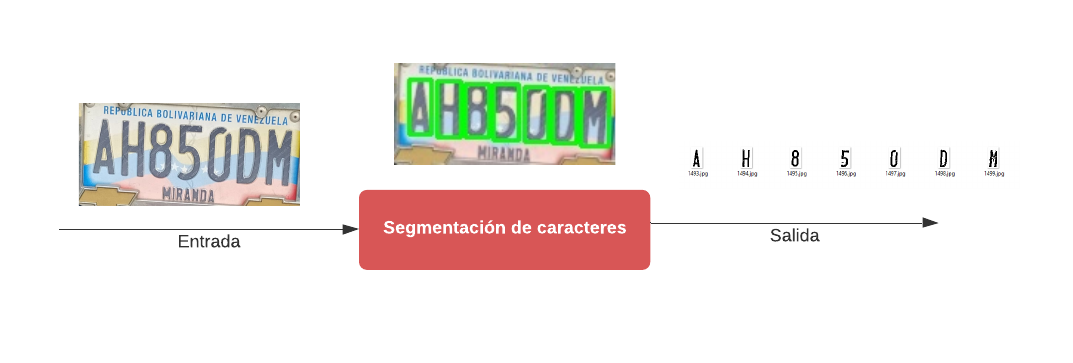
\includegraphics[width=0.7\linewidth]{Imagenes/segmentacion}
	\caption{ACA VA OTRA IMAGEN}
	\label{fig:segmentacion}
\end{figure}




\section{Componentes del sistema}

Se busca recrear de manera computarizada el proceso de observar una placa y leer su informaci�n. Por ello, se cuenta con una serie de herramientas y t�cnicas desarrolladas en Machine Learning y Visi�n Computarizada. La detecci�n de texto basado en el aprendizaje profundo de m�quinas, el procesamiento de im�genes con OpenCV el filtrado de la informaci�n y por �ltimo la M�quina de Soporte Vectorial imitar� el reconocimiento de caracteres, cumpliendo as� con los objetivos planteados. 

Dado lo anterior, se necesitar�: un computador d�nde se ejecutar� el algoritmo del proyecto y una base de datos compuesta por un conjunto de im�genes de caracteres que conformar�n el set de entrenamiento. Dado que el presente proyecto consiste en el dise�o de software, no contempla la captura de escenas.   Las pruebas se realizar�n con tomas previamente capturadas en condiciones controladas tanto en iluminaci�n como en la posici�n del objeto. Con lo anterior expuesto, el �nico componente f�sico que se requiere es un  computador. 


\section{Computador.}

Este proyecto, al tratarse de un dise�o de software, requiere �nicamente de un computador con las capacidades de computo suficientes para manejar los procedimientos l�gicos y matem�ticos que componen al algoritmo. Por lo tanto, no es necesario el uso de equipos especializados para su desarrollo.

El computador es una m�quina Toshiba Satellite C55 Series. El sistema operativo es Microsoft Windows 10. Las principales caracter�sticas del computador se describen en la tabla \ref{Tab:computo}:



\begin{table}[H]
	\centering
	\caption{Especificaciones del computador Toshiba Satellite C55 Series}\label{Tab:computo}
	\begin{tabular}{llr}
		\toprule
		Alimentaci�n &  19V \\

		Procesador & AMD QUAD-CORE A6 \\ 

		Memoria RAM & 16GB \\ 
		
		Tipo de sistema operativo & 64 bits \\ 
		\bottomrule
	\end{tabular}
\end{table}


\section{Base de datos}

En general, existen n�merosas bases de datos de matr�culas veh�culares de diferentes pa�ses del mundo y estas incluyen fotos de la placa completa. Es por ello que no es posible emplearlas para el entrenamiento de la M�quinas de Soporte Vectorial tomando en cuenta los objetivos del presente proyecto. 

Para cumplir con los requerimientos planteados, es fundamental contar con una base de datos compuesta por im�genes de todas las letras y n�meros del abecedario espa�ol individualmente. Es decir, cada imagen debe contener solo un tipo de car�cter. Por lo tanto, para entrenar la SVM fue necesario construir dicha base de datos.

Se construy� una base de datos que cuenta con 1496 im�genes de caracteres de letras y n�meros. Para su construcci�n se recopil� al menos 250 fotos de placas veh�culares de origen Venezolano y se procesaron utilizando herramientas provistas por la librer�a OpenCV, a fin de obtener la informaci�n de inter�s. 

Las t�cnicas empleadas para su construcci�n se basan en la detecci�n de contornos a partir de la umbralizaci�n de la imagen. Empleando diferentes funciones del procesamiento de im�genes y l�gica condicional en la programaci�n, se detectaron los caracteres de inter�s y se extrajeron recortando la foto. Las medidas adecuadas para su extracci�n se obtuvieron a partir de la medici�n del aspect ratio y el �rea ocupada por el car�cter en la foto, conservando una distancia prudencial entre los bordes y el car�cter . El resultado de la construcci�n result� en im�genes de 25 x 45 px, en blanco y negro.

El almacenamiento de cada uno de los ejemplos de entrenamiento se realiz� en un archivo .csv, el cual permiti� registrar en forma de matriz todos los ejemplos de entrenamiento. Para generar dicha matriz se redujo a�n m�s el tama�o de la imagen que contiene cada muestra, resultado en una imagen de 27 x 15 px, lo cual se traduce en 405 pixeles por muestra. De esta forma, cada fila de la matriz contenida en el archivo .csv corresponde a un ejemplo de entrenamiento individual. La �ltima columna de una fila corresponde a la etiqueta que identifica el car�cter de esa imagen. Para la escritura de este archivo se emple� la librer�a csv provista por Python.

En el dise�o, una de las mayores dificultades fue la construcci�n de la base de datos, ya que fue necesario  ajustar diferentes par�metros en el proceso de extracci�n de las muestras. Por otro lado, la adquisici�n de tantas placas Venezolanas represent� una gran dificultad, dado que fue debi� tomar todas las fotos y no se dispon�a el acceso a tantas placas de manera inmediata o en la red. Es por esto, que se cuenta con un n�mero limitado de ejemplos de entrenamiento en comparaci�n a los n�meros comunes, que por lo general superan el mill�n de muestras.

\begin{figure}[H]
	\centering
	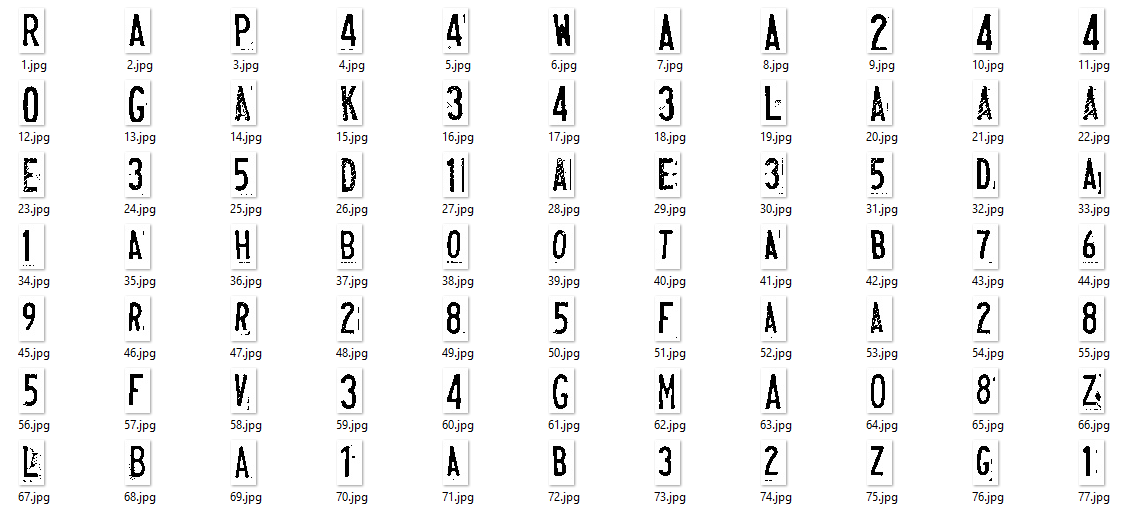
\includegraphics[width=0.7\linewidth]{Imagenes/data_base}
	\caption{Muestras de im�genes del set e entrenamientos creada.}
	\label{fig:database}
\end{figure}

La cantidad de muestras  extra�das por cada clasificaci�n se muestra en la Tabla \ref{Tab:tags}:


\begin{table}[H]
	\centering
	\caption{Clasificaci�n y etiquetas de cada car�cter.}\label{Tab:tags}
	\begin{adjustbox}{center, width=\columnwidth-10pt}  
		
	\begin{tabular}{llr}
		\toprule
		Clasificaci�n & Etiqueta & Cantidad extra�da \\ 
		\midrule
			0&0&46 \\
			
			1&1&43 \\
			
			2&2&71 \\
			
			3&3&54 \\
			
			4&4&66 \\
			
			5&5&50 \\
			
			6&6&72 \\
			
			7&7&65	\\
			
			8&8&58	\\
			
			9&9&70	\\
			
			A&10&297 \\
			
			B&11&65 \\
			
			C&12&38	\\
			
			D&13&51	\\
			
			E&14&37	\\
			
			F&15&43	\\
			
			G&16&52	\\
			
			H&17&26	\\
			
			I&18&18	\\
			
			J&19&10	\\
			
			K&20&28	\\
			
			L&21&13	\\
			
			M&22&46	\\
			
			N&23&16	\\
			
			�&-&-	\\
			
			O&24&28	\\
			
			P&25&12	\\
			
			Q&26&0	\\
			
			R&27&18	\\
			
			S&28&8	\\
			
			T&29&5	\\
			
			U&30&13	\\
			
			V&31&23	\\
			
			W&32&13	\\
			
			X&33&18	\\
			
			Y&34&12	\\
			
			Z&35&7	\\
		\bottomrule
	\end{tabular}
\end{adjustbox}
\end{table}


\section{Software}

El proyecto tiene como objeto dise�ar un sistema que permita el reconocimiento de la matr�cula de un veh�culo en una imagen est�tica, por lo tanto los videos no est�n contemplados en este dise�o.

Dado que el objetivo es reconocer la informaci�n contenida en la matr�cula de un veh�culo, el software debe tener la capacidad de extraer los caracteres de inter�s contenidos en la placa mediante el procesamiento de im�genes y luego clasificar cada uno de ellos. 

\begin{figure}[H]
	\centering
	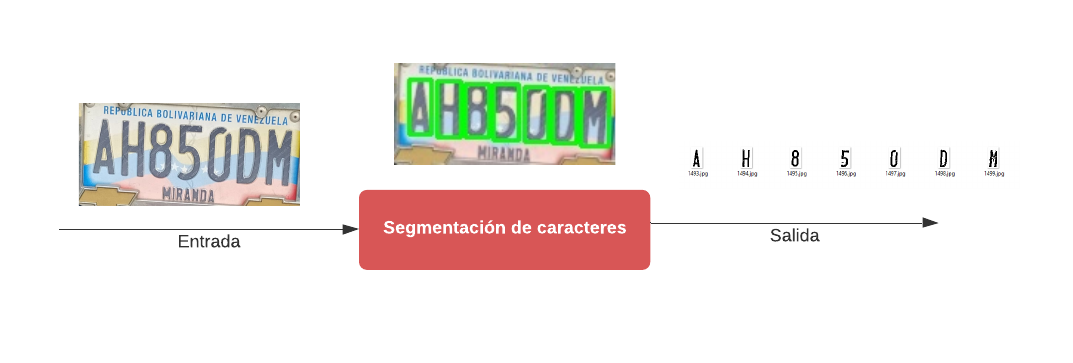
\includegraphics[width=0.7\linewidth]{Imagenes/segmentacion}
	\caption{Proceso de segmentaci�n de caracteres.}
	\label{fig:segmentacion}
\end{figure}


Para lograr lo anterior, se emple�  Python3, la librer�a OpenCV de Intel.


As�, es posible las etapas del software en los siguientes m�dulos:

\begin{itemize}
	
	\item Detecci�n de la placa trav�s de t�cnicas de procesamiento de im�genes. 
	
	\item Segmentaci�n de los caracteres mediante el procesamiento de im�genes.
	
	\item Clasificaci�n de los caracteres empleando machine learning.
	
\end{itemize} 



\subsection{Detecci�n de la placa}

El m�dulo de detecci�n de la placa se define como un sistema d�nde se ingresa una imagen frontal o posterior  de un veh�culo y se obtiene la placa contenida. Se puede describir este proceso en las siguientes etapas:

\begin{itemize}
	
	\item Localizaci�n.
	
	\item Extracci�n.
	
\end{itemize}

De esta forma, es necesario emplear t�cnicas o herramientas que permitan detectar la localizaci�n de la placa. Considerando que la placa contiene texto, es posible utilizar t�cnicas avanzadas como los detectores de texto, como por ejemplo m�quinas de aprendizaje basadas en aprendizaje profundo. Estas herramientas creadas a partir de Machine Learning, permiten detectar el texto en una imagen seg�n las caracter�sticas de su entrenamiento.

El modelo EAST es un detector de texto basado en el aprendizaje profundo y OpenCV. Dado que el objeto del presente proyecto es reconocer los caracteres de la placa, es posible emplear m�dulos de detecci�n de texto ya desarrollados. Se emple� el modelo EAST  para detectar la localizaci�n de la placa en la fotograf�a y, tomando en consideraci�n el �rea de la placa, se extrae el contenido de inter�s. 

\subsection{Segmentaci�n de los caracteres.}


El m�dulo de segmentaci�n se encarga de detectar y extraer los caracteres de inter�s dentro de la placa. Esto se realiz� mediante t�cnicas de procesamiento de im�genes mediante la librer�a la librer�a OpenCV. Se describe  dicho proceso en el siguiente diagrama de flujo:

\begin{figure}[H]
	\centering
	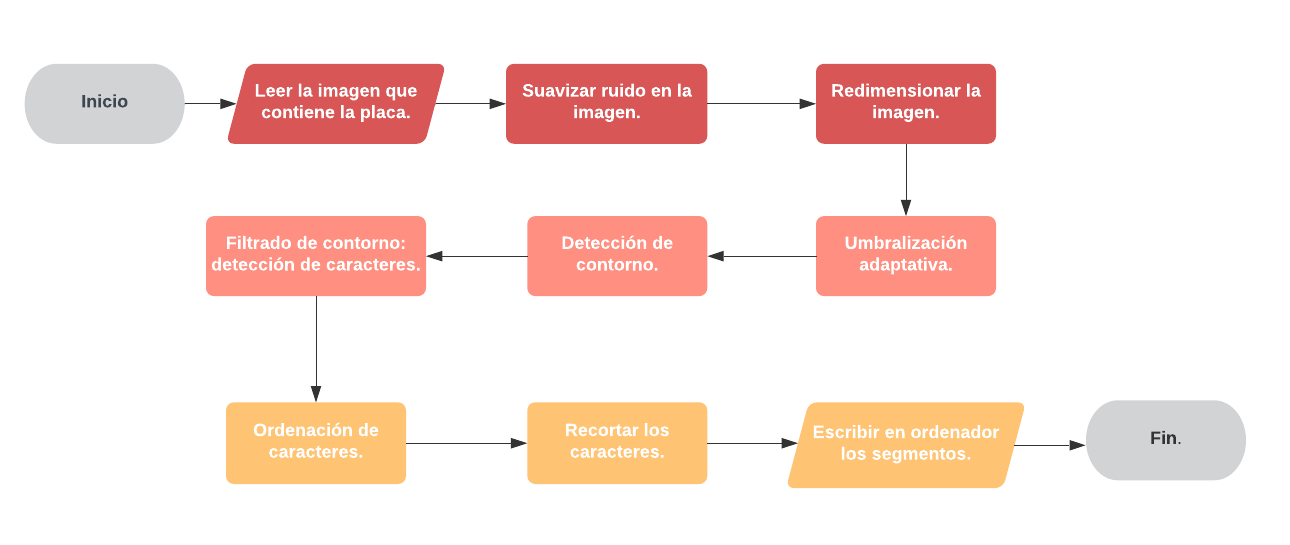
\includegraphics[width=1\linewidth]{Imagenes/Segmentacion_caracter_diagrama}
	\caption{Proceso de segmentaci�n de los caracteres de una matr�cula.}
	\label{fig:segmentacioncaracterdiagrama}
\end{figure}


\begin{enumerate}
	
	
	\item \textbf{Suavizado de ruido:} En primer lugar, es necesario suavizar el ruido de la imagen que contiene la placa limpi�ndola de caracter�sticas no deseadas. Una caracter�stica no deseada puede aparecer debido a que la placa f�sicamente posee desperfectos que intervienen significativamente en la detecci�n de contornos o, por otro lado, si la fotograf�a es tomada fuera de las condiciones ideales. Para realizar esto se suaviz� el ruido con un kernel gaussiano mediante la funci�n \verb|cv2.GaussianBlur()|.
	
	\item \textbf{Redimensionamiento de la imagen:} La imagen que contiene la placa es redimensionada hasta obtener 150px de altura, posteriormente permitir� que el algoritmo pueda detectar y extraer los caracteres en segmentos  de 25 x 45 px. En general, los ejemplos de entrenamiento son contenidos en im�genes de dimensiones peque�as considerando que cada pixel que la compone es una caracter�stica de entrada para el algoritmo, lo cual significa un importante costo computacional. Para lograr el redimensionamiento se emple� fundamentalmente la funci�n \verb|cv2.rezise()|. 
	
	\item \textbf{Umbralizaci�n de la imagen:} La umbralizaci�n se realiza con el fin de binarizar la imagen. Para la detecci�n de contornos es imprescindible que la binarizaci�n sea inversa. De esta forma, los contornos detectados son colocados en blanco y el fondo en negro. En este proyecto se utiliz� umbralizaci�n adaptativa \verb|cv2.adaptativetresholding()|. La umbralizaci�n adaptativa es una funci�n que a partir de los par�metros ingresados binariza considerando peque�as regiones de la imagen, a diferencia de una umbralizaci�n estandar. Por lo tanto, la umbralizaci�n adaptativa c�lcula el valor umbral adecuado para cada regi�n, mediante un kernel gaussiano. Es importante que la umbralizaci�n sea adaptable por regi�n ya que factores externos como la iluminaci�n pueden afectar significativamente el proceso de binarizaci�n.
	
	\item \textbf{Detecci�n de contorno:} La detecci�n de contornos se aplica sobre la imagen umbralizada, d�nde ya la mayor�a del ruido ha sido filtrado. En este paso, se utiliz� la funci�n \verb|cv2.findcontours()| la cu�l retorna una variable que contiene los contornos detectados. La detecci�n de los contornos de la imagen depende de los par�metros ingresados en la funci�n. En este caso, se detectan los contornos cerrados en la imagen.
	
	\item \textbf{Filtraci�n de contornos:} La filtraci�n de contorno consiste en seleccionar los contornos de inter�s. Se emple� l�gica condicional a fin de verificar si el contorno clasifica o no. Para ello, se estim� el �rea y el aspect ratio que ocupa un caracter dentro de la placa. Se ponderaron los valores de ancho y alto de varias muestras para obtener un valor umbral. As�, se defini� una relaci�n porcentual del �rea del car�cter respecto al �rea de la placa y un bias que permita cubrir la mayor�a de las variaciones. De esta forma se estableci� el filtro de contornos d�nde se detectan los caracteres de la matr�cula. Para obtener las coordenadas de los caracteres se utiliz� la funci�n \verb|cv2.boundingrectangle()|, la cual permite encerrar en rect�ngulos los contornos detectados y devuelve los valores que permiten definir su posici�n en la imagen.
	
	\item \textbf{Recorte de los caracteres:} Con las coordenadas de los caracteres, se extrajeron recortando la imagen con un margen de provisi�n adecuado. As�, se asegur� contener completamente cada caracter en un segmento. Para la recortar la imagen se usaron las funciones b�sicas de Python, que consiste en extraer un segmento de la imagen a partir de unas coordenadas dadas.
	
	\item \textbf{Escritura en computador de los caracteres:} Una vez obtenido todos los segmentos se escriben en el computador utilizando \verb|cv2.imwrite()|, con formato .jpg.
	
	
	
\end{enumerate}


\subsection{Clasificaci�n de caracteres.}






\newpage



%==================================================================
\chapter{PRUEBAS Y RESULTADOS}\label{CAP:exp}
%\markboth{Tu Segundo Cap?tulo}{Tu Segundo Cap?tulo}%

% !TeX spellcheck = es_ES
% !TeX encoding = ISO-8859-1

Una vez dise�ados e implementados los m�dulos de detecci�n de placa, detecci�n de caracteres y reconocimiento de caracteres se realizaron diferentes pruebas que permiten evaluar el desempe�o del sistema  y validar su funcionamiento, as� como definir las condiciones bajo los cuales se obtiene los �ptimos resultados en cu�nto a detecci�n y clasificaci�n. 

 \section{Desempe�o del sistema}
 
 Para medir el desempe�o del sistema en cada uno de sus m�dulos as� como en su funcionamiento global se probaron 2 escenarios: reconocimiento de caracteres que participaron en la base de datos y reconocimiento de caracteres que no participaron en la base de datos. 
 
 En un sistema real la entrada al sistema es capturada por un dispositivo instalado en posici�n y espacio fijo, por lo que todas las entradas se encuentran sometidas a las mismas condiciones controlables. Por lo que una vez ajustada la resoluci�n de la c�mara se cuenta con entradas que tienen caracter�sticas muy similares. Para la realizaci�n de dichas pruebas la entrada al sistema fue con im�genes a diferentes resoluciones, �ngulo de captura y distancia dado que no se dispone de un sistema f�sico real que obtenga entradas uniformes. Esto sucede especialmente en los ejemplos de entrenamiento que componen la base de datos. Es importante recalcar que el cambio de resoluci�n en una captura podr�a significar una p�rdida de informaci�n importante que incide directamente en el correcto reconocimiento del car�cter, ya que su vector de caracter�stica es directamente afectado. Por otro lado, la variaci�n del �ngulo de captura genera distorsi�n en las im�genes por lo que tambi�n incide directamente en la clasificaci�n de caracteres, producto de la variaci�n en el vector de medida. 
 
 \subsection{Reconocimiento de caracteres que forman parte de la base de datos}
 
 En esta prueba no fue posible evaluar el m�dulo de detecci�n de placa ya que las muestras disponibles son directamente una foto de la placa sin considerar el resto del autom�vil. Por lo que se evaluar� el desempe�o de la detecci�n de car�cter y clasificaci�n de la misma. 
 
 Se tomaron aleatoriamente 50 de las 250 placas que se obtuvieron para la construcci�n de la base de datos, a fin de evaluar el rendimiento de detecci�n y reconocimiento de caracteres ya conocidos por el algoritmo.
 

 
 \begin{figure}[H]
 	\centering
 	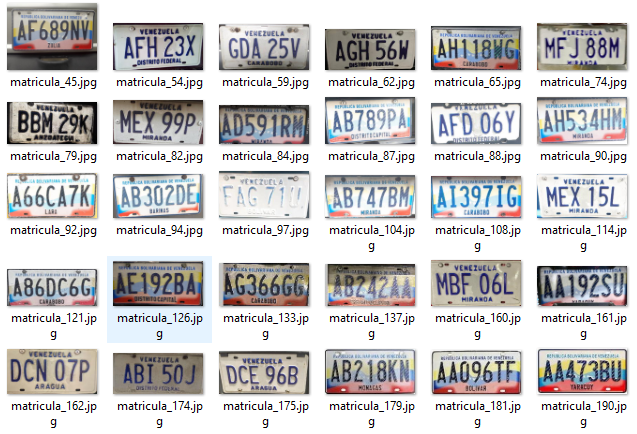
\includegraphics[width=0.7\linewidth]{Imagenes/Prueba1_DB}
 	\caption{Placas que participaron en la construcci�n de la base de datos.}
 	\label{fig:prueba1db}
 \end{figure}

 

\begin{figure}[H]
	\centering
	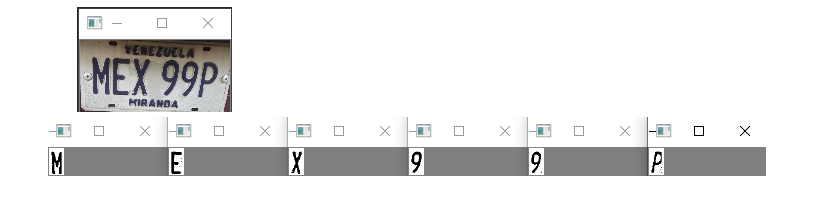
\includegraphics[width=0.7\linewidth]{Imagenes/placaext_82DB}
	\caption{Procesamiento de la placa 82 de la base de datos.}
	\label{fig:placaext82db}
\end{figure}

\begin{figure}[H]
	\centering
	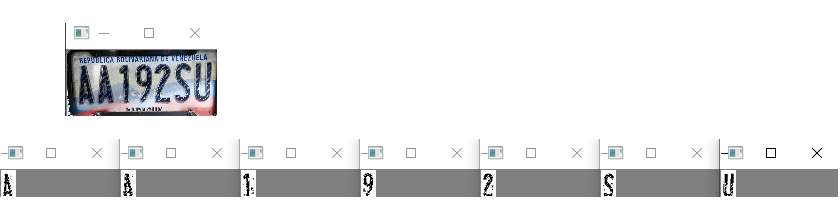
\includegraphics[width=0.7\linewidth]{Imagenes/placaext_161DB}
	\caption{Procesamiento de la placa 161 de la base de datos.}
	\label{fig:placaext161db}
\end{figure}

\begin{figure}[H]
	\centering
	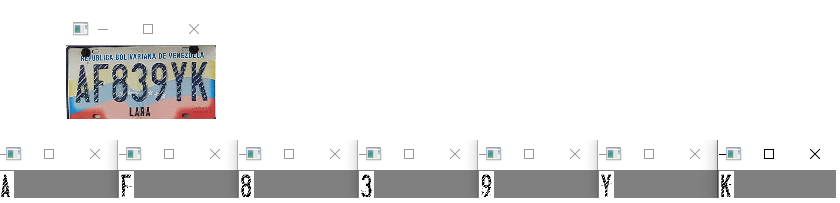
\includegraphics[width=0.7\linewidth]{Imagenes/placaext_229DB}
	\caption{Procesamiento de la placa 229 de la base de datos.}
	\label{fig:placaext229db}
\end{figure}

El m�dulo reconoci� en su mayor�a  los caracteres de las placas realizando correctamente las extracciones como se puede observar en las Figuras \ref{fig:placaext82db}, \ref{fig:placaext161db} y \ref{fig:placaext229db}. Se observa en la parte superior de las  figuras la placa a la cual corresponde la extracci�n.

\begin{figure}[H]
	\centering
	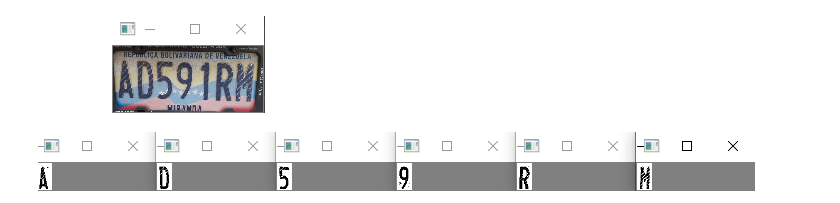
\includegraphics[width=0.7\linewidth]{Imagenes/placaext_84EDB}
	\caption{Procesamiento de la placa 84 de la base de datos}
	\label{fig:placaext84edb}
\end{figure}

\begin{figure}[H]
	\centering
	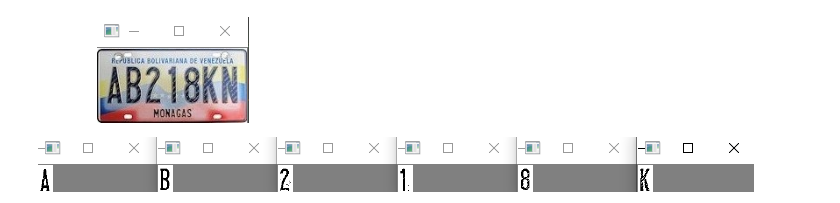
\includegraphics[width=0.7\linewidth]{Imagenes/placaext_179EDB}
	\caption{Procesamiento de la placa 179 de la base de datos}
	\label{fig:placaext179edb}
\end{figure}

\begin{figure}[H]
	\centering
	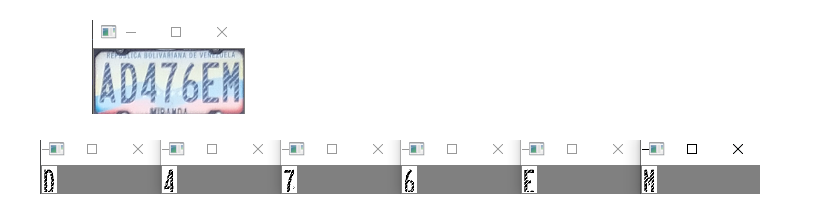
\includegraphics[width=0.7\linewidth]{Imagenes/placaext_243EDB}
	\caption{Procesamiento de la placa 243 de la base de datos}
	\label{fig:placaext243edb}
\end{figure}

Por otro lado, en las Figuras \ref{fig:placaext84edb}, \ref{fig:placaext179edb} y \ref{fig:placaext243edb} son algunos de los casos d�nde el M�dulo de detecci�n de caracteres detect� err�neamente y por lo tanto se considera un fallo. El resultado de estas muestras son clasificado c�mo errores debido a que fallaron en detectar algunas de las letras de la placa.En las placas Venezolanas se pueden hallar de 6 a 7 caracteres dependiendo del a�o en que fueron fabricadas. En consecuencia, si el m�dulo de detecci�n de caracteres no detecta al menos 6 contornos que cumplan con las caracter�sticas arroja fallo en la detecci�n general. Experimentalmente se encontr� que este tipo de errores se originan en la detecci�n de contornos del sistema y usualmente se debe  a una combinaci�n de factores externos e internos. 

Los factores externos que indicen significativamente en la detecci�n de contornos frecuentemente es la iluminaci�n, �ngulo de captura y condiciones de preservaci�n del cuerpo f�sico matr�cula. Los factores internos hacen referencia a los par�metros o procedimientos del procesamiento de imagenes. Una soluci�n para reducir al m�nimo los factores externos es implementar un sistema f�sico que permita tomar capturas a una misma resoluci�n, con un �ngulo de captura fijo y condiciones de iluminaci�n similares.

En la Figura \ref{fig:placaext179edb} es un caso que a simple vista se puede descartar a los factores externos como origen al problema. A�n as�, se obtuvo un fallo en la detecci�n general. El sistema realmente no es capaz de ver propiamente la matr�cula, este compara matem�ticamente dos valores y toma una decisi�n en base a eso. Entonces esta detecci�n se origina debido a un factor interno. Para realizar la detecci�n de contornos el sistema recorre la imagen mediante un Kernel en el proceso de umbralizaci�n. A pesar que la Umbralizaci�n es adaptable por zonas, el tama�o del Kernel con el que recorre la im�gen no lo es. En este proyecto el tama�o del kernel se estableci� en 15 pixeles. Una posible soluci�n podr�a ser considerar diferentes tama�os para obtener mejores resultados. Adicionalmente, en el reconocimiento de caracteres el algoritmo clasific� la K como una A. Este error puede deberse a que en la base de datos exista un ejemplo que matem�ticamente los valores introducidos al modelo por medio de la extracci�n  de caracter�sticas coincidan con los de la letra K de esta placa. Este �ltimo se soluciona depurando la Base de Datos de los ejemplos que puedan ocasionar este tipo de errores.

En la Figura \ref{fig:placaext243edb} los inconvenientes se presentan en forma similar al anterior, pero es importante destacar que en la extracci�n se puede observar que los contornos superan las medidas l�mites de los cuadros como es el caso particular de la letra D y E. A pesar de lo anterior, el sistema de reconocimiento fue capaz de reconocer la letra D, sin embargo, la letra E la clasific� con una F. Este problema de reconocimiento no se origina en el modelo del algoritmo SVM sino en la extracci�n de caracteres. Su soluci�n recae en mejorar el rendimiento de extracci�n de caracteres.

A continuaci�n se presenta la Tabla \ref{Tab:prueba1} d�nde se registr� la placa, caracteres detectados y reconocidos a fin de evaluar su desempe�o:

\begin{table}[H]
	\centering
	\caption{Lista de placas que participaron en la prueba.}\label{Tab:prueba1}
	\begin{tabular}{lccc}
		\toprule
		Placa ID & N�mero de Placa  & Detectados & Reconocidos \\
		\midrule
		82&MEX99P&MEX99P&MEX99P \\
		45&AF689NV&AF689NV&AF689NV \\
		244&AJ294OA&AJ294OA&AJ294OA \\
		162&DCN07P&DCN07P&DCN07P \\
		121&A86DC6G&A86DC6G&A86DC6G \\
		248&AB275UN&AB275UN&AB275UN \\
		161&AA192SU&AA192SU&AA192SU \\
		192&A05DJ4G&A05DJ4G&A05DJ4G \\
		175&DCE96B&DCE96B&DCE96B \\
		88&AFD06Y&AFD06Y&AFD06Y \\
		62&AGH56W&AGH56W&AGH56W \\
		204&AA251MD&AA25MD&AA25HD \\
		241&AB076DF&AB076DF&AB076DF \\
		133&AG366GG&AG366GG&AG366GG \\
		197&DBM43M&DBM43M&DBM43M \\
		90&AH534HM&AH534HM&AH534HM \\
		79&BBM29K&BBM29K&BBM29K \\
		84&AD591RM&AD59RM&AD59RM \\
		238&A00CG8V&A00CG8V&A00CG8V \\
		160&MBF06L&MBF06L&MBF06L \\
		104&AB747BM&AB747BM&AB747BM \\
		217&AF283VG&AF283VG&AF283VG \\
		74&MFJ88M&MFJ88M&MFJ88M \\
		108&AI397IG&AI397IG&AI397IG \\
		249&AK179GA&AK179GA&AK179GA \\
		65&AH118WG&AH118WG&AH118WG \\
		94&AB302DE&AB302DE&AB302DE \\
		219&ABI37X&ABI37X&ABI37X \\
		242&MAC24A&MAC24A&MAC24A \\
		87&AB789PA&AB789PA&AB789PA \\
		92&A66CA7K&A66CA7K&A66CA7K \\
		190&AA473BU&AA473BU&AA473BU \\
		56&AF834EG&AF834EG&AF834EG \\
		243&AD476EM&D476EM&D476FM \\
		54&AFH23X&AFH23X&AFH23X \\
		137&AB242AA&B242AA&B242AA \\
		181&AA096TF&AA096TF&AA096TF \\
		174&ABI50J&ABI50J&ABI50J \\
		228&AL092BA&AL092BA&AL092BA \\
		114&MEX15L&MEX15&MEX15L \\
		251&AH850DM&AH850DM&AH850DM \\
		126&AE192BA&AE192BA&AE192BA \\
		179&AB218KN&AB218K&AB218A \\
		229&AF839YK&AF839YK&AF839YK \\
		234&AA453UD&AA45UD&AA45UD \\
		\bottomrule
	\end{tabular}
\end{table}

El sistema fall� en la detecci�n de caracteres de 7 placas de 50. Este fallo se origina debido a que el M�dulo de detecci�n de caracteres no logr� encontrar al menos 6 caracteres dentro de la matricula.

\begin{table}[H]
	\centering
	\caption{Desempe�o con muestras de la base de datos.}\label{Tab:pruebas1e}
	\begin{tabular}{lccc}
		\toprule
		Car�cter & Tasa de �xito  & Detectados & Reconocidos \\
		\midrule
		0 & 1.0 & 12 & 12 \\
		1 & 1.0 & 7 & 7 \\
		2 & 1.0 & 14 & 14 \\
		3 & 1.0 & 11 & 11 \\
		4 & 1.0 & 11 & 11 \\
		5 & 1.0 & 10 & 10 \\
		6 & 1.0 & 14 & 14 \\
		7 & 1.0 & 12 & 12 \\
		8 & 1.0 & 12 & 12 \\
		9 & 1.0 & 15 & 15 \\
		A & 1.0 & 49 & 49 \\
		B & 1.0 & 18 & 18 \\
		C & 1.0 & 6 & 6 \\
		D & 1.0 & 13 & 13 \\
		E & 0.857 & 7 & 6 \\
		F & 1.0 & 10 & 10 \\
		G & 1.0 & 12 & 12 \\
		H & 1.0 & 6 & 6 \\
		I & 1.0 & 4 & 4 \\
		J & 1.0 & 4 & 4 \\
		K & 0.8 & 5 & 4 \\
		L & 1.0 & 2 & 2 \\
		M & 0.933 & 15 & 14 \\
		N & 1.0 & 3 & 3 \\
		O & 1.0 & 1 & 1 \\
		P & 1.0 & 3 & 3 \\
		Q & 0 & 0 & 0 \\
		R & 1.0 & 1 & 1 \\
		S & 1.0 & 1 & 1 \\
		T & 1.0 & 1 & 1 \\
		U & 1.0 & 4 & 4 \\
		V & 1.0 & 3 & 3 \\
		W & 1.0 & 2 & 2 \\
		X & 1.0 & 4 & 4 \\
		Y & 1.0 & 2 & 2 \\
		Z & 0 & 0 & 0 \\
		\bottomrule
	\end{tabular}
\end{table}

En la Tabla \ref{Tab:pruebas1e} se puede observar las anal�ticas obtenidas de un n�mero total de 50 muestras que participaron en el entrenamiento de la base de datos. En este experimento se obtuvo una tasa de �xito de 0.844 en la detecci�n de caracteres. Mientras que en el rendimiento de reconocimiento de caracteres obtuvo una tasa de �xito 0.989. 

 

\subsection{Reconocimiento de caracteres que no forman parte de la base de datos}

Para esta prueba se consideraron las siguientes condiciones: 2 metros de distancia respecto a la placa del autom�vil y un metro de altura respecto al suelo. Las condiciones de iluminaci�n eran tenues ya que los veh�culos se encontraban en un estacionamiento. Por lo tanto, teniendo en cuenta estas variables controladas se obtuvo la captura de 10 autom�viles diferentes para evaluar el desempe�o de detecci�n de placa, detecci�n de caracteres y reconocimiento de caracteres. 


\begin{figure}[H]
	\centering
	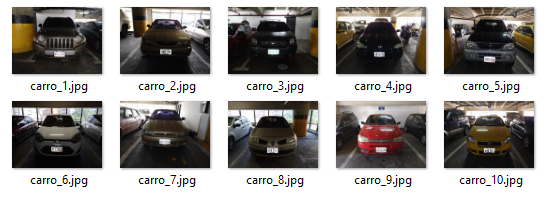
\includegraphics[width=0.7\linewidth]{Imagenes/Prueba2_CN}
	\caption{Placas que no participaron en la base de datos}
	\label{fig:prueba2cn}
\end{figure}


El primer m�dulo por evaluar es el \textit{M�dulo de detecci�n de placa}. Como se explic� en cap�tulos anteriores, el sistema buscar� dentro de la imagen un contorno que cumpla con la relaci�n de ancho y altura de una placa a la distancia de 2 metros. De los 10 veh�culos considerados en la Figura \ref{fig:prueba2cn} el m�dulo logr� detectar 9. Las placas detectadas se observan en la Figura \ref{fig:placascn}. 

\begin{figure}[H]
	\centering
	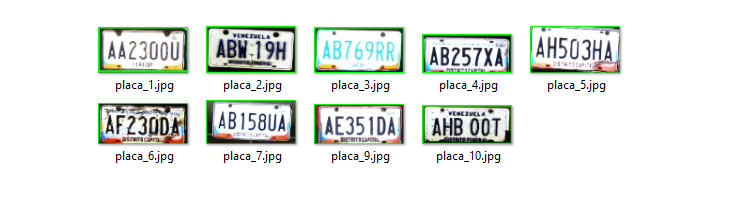
\includegraphics[width=0.7\linewidth]{Imagenes/placas_CN}
	\caption{Resultado del \textit{M�dulo de detecci�n de placa} procesando entradas que no participaron en la base de datos.}
	\label{fig:placascn}
\end{figure}


\begin{table}[H]
	\centering
	\caption{Desempe�o en la detecci�n de placas.}\label{Tab:pruebas}
	\begin{tabular}{cccc}
		\toprule
		Placas detectadas & Placas no detectadas  & N�mero total de placas & Tasa de �xito \\
		\midrule
		9 & 1 & 10 & 0.9\\
		\bottomrule
	\end{tabular}
\end{table}

De esta forma, el sistema contin�a hasta la detecci�n de caracteres. De las 9 placas ingresadas al siguiente m�dulo se detectaron todos los caracteres. Los resultados de detecci�n se presentan a continuaci�n:
 
 \begin{figure}[H]
 	\centering
 	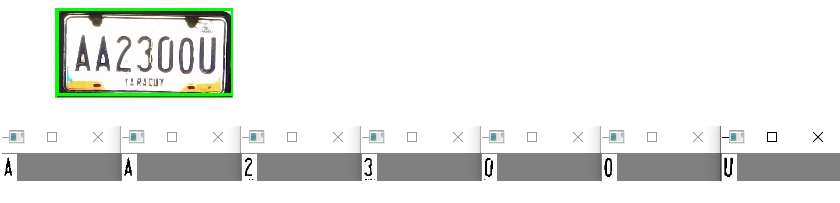
\includegraphics[width=0.7\linewidth]{Imagenes/extraccar1}
 	\caption{Extracci�n de caracteres de la placa 1}
 	\label{fig:extraccar1}
 \end{figure}
 
 \begin{figure}[H]
 	\centering
 	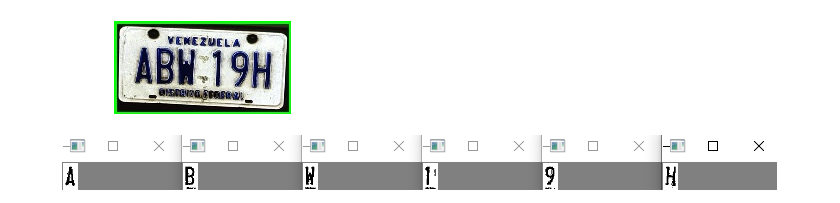
\includegraphics[width=0.7\linewidth]{Imagenes/extraccar2}
 	\caption{Extracci�n de caracteres de la placa 2}
 	\label{fig:extraccar2}
 \end{figure}
 
 \begin{figure}[H]
 	\centering
 	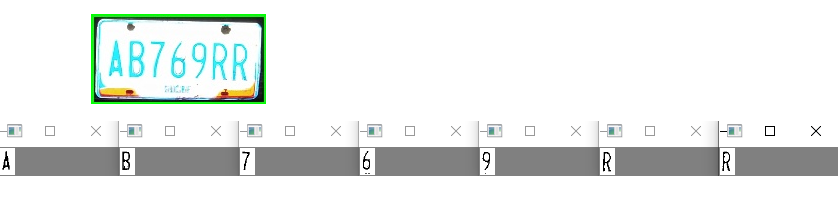
\includegraphics[width=0.7\linewidth]{Imagenes/extraccar3}
 	\caption{Extracci�n de caracteres de la placa 3}
 	\label{fig:extraccar3}
 \end{figure}
 
 \begin{figure}[H]
 	\centering
 	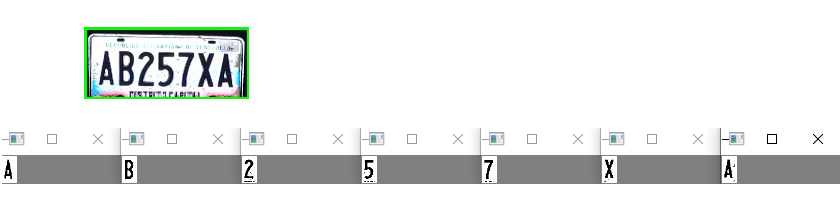
\includegraphics[width=0.7\linewidth]{Imagenes/extraccar4}
 	\caption{Extracci�n de caracteres de la placa 4}
 	\label{fig:extraccar4}
 \end{figure}
 \begin{figure}[H]
 	\centering
 	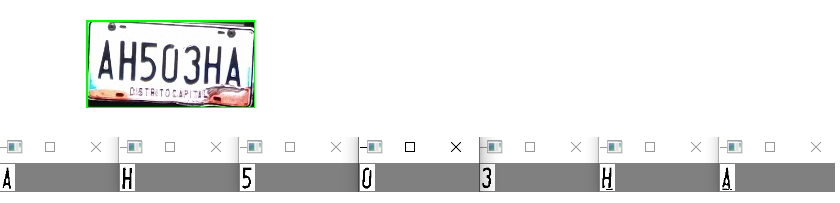
\includegraphics[width=0.7\linewidth]{Imagenes/extraccar5}
 	\caption{Extracci�n de caracteres de la placa 5}
 	\label{fig:extraccar5}
 \end{figure}
 
 \begin{figure}[H]
 	\centering
 	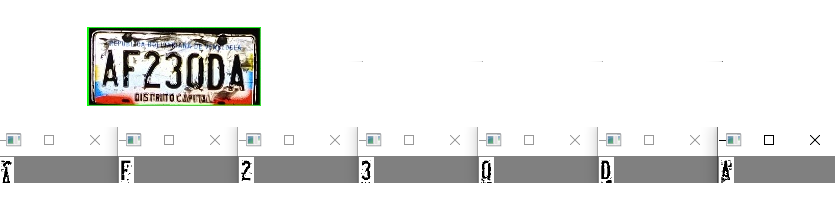
\includegraphics[width=0.7\linewidth]{Imagenes/extraccar6}
 	\caption{Extracci�n de caracteres de la placa 6}
 	\label{fig:extraccar6}
 \end{figure}

 \begin{figure}[H]
 	\centering
 	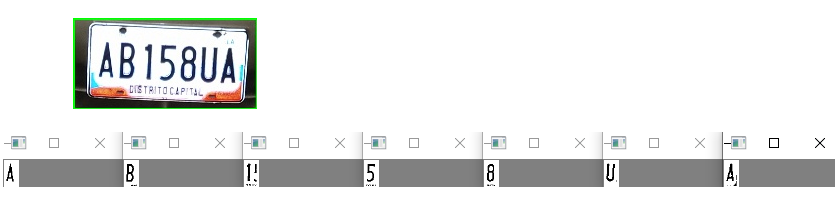
\includegraphics[width=0.7\linewidth]{Imagenes/extraccar7}
 	\caption{Extracci�n de caracteres de la placa 7}
 	\label{fig:extraccar7}
 \end{figure}
 
 \begin{figure}[H]
 	\centering
 	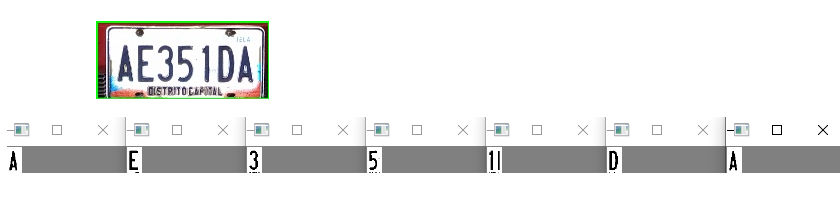
\includegraphics[width=0.7\linewidth]{Imagenes/extraccar9}
 	\caption{Extracci�n de caracteres de la placa 9}
 	\label{fig:extraccar9}
 \end{figure}
 
 \begin{figure}[H]
 	\centering
 	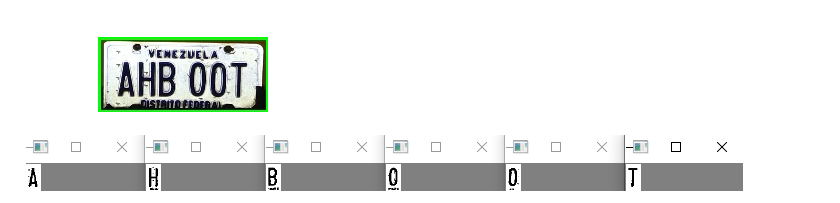
\includegraphics[width=0.7\linewidth]{Imagenes/extraccar10}
 	\caption{Extracci�n de caracteres de la placa 10}
 	\label{fig:extraccar10}
 \end{figure}
 
 A continuaci�n se presenta la Tabla \ref{Tab:prueba2} d�nde se registr� la placa, caracteres detectados y reconocidos a fin de evaluar su desempe�o:
 
  \begin{table}[H]
 	\centering
 	\caption{Desempe�o con nuevas entradas }\label{Tab:prueba2}
 	\begin{tabular}{lccc}
 		\toprule
 		Placa ID & N�mero de Placa& Detectados & Reconocidos \\
 		\midrule
		1&AA230OU&AA230OU&AA230OU \\
		2&ABW19H&ABW19H&ABW19H \\
		3&AB769RR&AB769RR&AB769RR \\
		4&AB257XA&AB257XA&AB257XA \\
		5&AH503HA&AH503HA&AH503HA \\
		6&AF230DA&AF230DA&XF23ODA \\
		7&AB158UA&AB158UA&AB158UA \\
		9&AE351DA&AE351DA&AE351DA \\
		10&AHB00T&AHB00T&AH8007 \\
 		\bottomrule
 	\end{tabular}
 \end{table}
 
 Se observa que la placa de la figura \ref{fig:extraccar6} el algoritmo no reconoci� correctamente el n�mero 0 clasific�ndolo como una O. Este error ocurri� debido a los factores externos que afectan las caracter�sticas f�sicas de la placa. Como se puede notar esta placa se encuentra bastante deteriorada por lo que las manchas agregan bastante ruido para el algoritmo de reconocimiento. Las irregularidades f�sicas que se aprecian matricula indicen significativamente en el procesamiento de imagen para la detecci�n de contornos en el �rea de la placa. En consecuencia, la detecci�n del contorno como en el primer car�cter se ve influenciado por las manchas alrededor y provoca una incorrecta extracci�n.
 
 \begin{table}[H]
	\centering
	\caption{Desempe�o con nuevas entradas }\label{Tab:producion}
	\begin{tabular}{lccc}
		\toprule
		Car�cter & Tasa de exito & Detectados & Reconocidos \\
		\midrule
		0 & 0.8 & 5 & 4 \\
		1 & 1.0 & 3 & 3 \\
		2 & 1.0 & 3 & 3 \\
		3 & 1.0 & 4 & 4 \\
		4 & 0 & 0 & 0 \\
		5 & 1.0 & 4 & 4 \\
		6 & 1.0 & 1 & 1 \\
		7 & 1.0 & 2 & 2 \\
		8 & 1.0 & 1 & 1 \\
		9 & 1.0 & 2 & 2 \\
		A & 0.933 & 15 & 14 \\
		B & 0.8 & 5 & 4 \\
		C & 0 & 0 & 0 \\
		D & 1.0 & 2 & 2 \\
		E & 1.0 & 1 & 1 \\
		F & 1.0 & 1 & 1 \\
		G & 0 & 0 & 0 \\
		H & 1.0 & 4 & 4 \\
		I & 0 & 0 & 0 \\
		J & 0 & 0 & 0 \\
		K & 0 & 0 & 0 \\
		L & 0 & 0 & 0 \\
		M & 0 & 0 & 0 \\
		N & 0 & 0 & 0 \\
		O & 1.0 & 1 & 1 \\
		P & 0 & 0 & 0 \\
		Q & 0 & 0 & 0 \\
		R & 1.0 & 2 & 2 \\
		S & 0 & 0 & 0 \\
		T & 0.0 & 1 & 0 \\
		U & 1.0 & 2 & 2 \\
		V & 0 & 0 & 0 \\
		W & 1.0 & 1 & 1 \\
		X & 1.0 & 1 & 1 \\
		Y & 0 & 0 & 0 \\
		Z & 0 & 0 & 0 \\
		\bottomrule
	\end{tabular}
\end{table}

  En la Tabla \ref{Tab:producion} se puede observar las anal�ticas obtenidas de las 10 capturas. La tasa de �xito obtenida en la detecci�n de car�cter fue de 1.0. Por otro lado, la tasa de �xito en el reconocimiento de caracteres es de  0.934 en reconocimiento de caracteres.
  
  \subsection{Tiempos de ejecuci�n}
  
  Otro aspecto crucial en la investigaci�n es el tiempo de entrenamiento de la SVM el cual fue de 1.29 para la base de datos constru�da y las carcter�sticas descritas del computador. 
  
  Por otro lado, en la Tabla \ref{Tab:prueba3}se puede observar los tiempos de procesamiento de imagenes y reconocimiento de caracteres obtenidos en la prueba de  \textit{Reconocimiento de caracteres que no forman parte de la base de datos}. 
  
  
    \begin{table}[H]
  	\centering
  	\caption{Tiempos de procesamiento y reconocimiento }\label{Tab:prueba3}
  	\begin{tabular}{lccc}
  		\toprule
  		Placa ID & N�mero de Placa& Procesamiento de imagen [s] & Reconocimiento de caracteres [s] \\
  		\midrule
  		1&AA230OU&0.839&0.338 \\
  		2&ABW19H&0.55&0.268 \\
  		3&AB769RR&0.577&0.252 \\
  		4&AB257XA&0.7&0.282 \\
  		5&AH503HA&0.954&0.365 \\
  		6&AF230DA&0.644&0.349 \\
  		7&AB158UA&0.665&0.396\\
  		9&AE351DA&0.655&0.214 \\
  		10&AHB00T&0.656&0.195 \\
  		\bottomrule
  	\end{tabular}
  \end{table}
  
  
  En promedio se obtiene que el tiempo de procesamiento de imagen es 0.624s y tiempo de reconocimiento de caracteres 0.266s. 

%==================================================================
\chapter{CONCLUSIONES}\label{CAP:conclu}
%\markboth{Tu Segundo Cap?tulo}{Tu Segundo Cap?tulo}%
%
% !TeX spellcheck = es_ES
% !TeX encoding = ISO-8859-1

 El procesamiento de im�genes es una tecnolog�a que permitir� la creaci�n de sistemas capaces de automatizar tareas que dar�n paso a una nueva sociedad tecnol�gica, como lo son los autom�viles no tripulados, reconocimiento de rostros, detecci�n de movimiento, entre otros. Lo anterior se logra obteniendo informaci�n de inter�s dentro de una captura de imagen mediante herramientas y procedimientos  matem�ticos. 

 
 
  Desarrollar el sistema en m�dulos independientes permiti�  probar diferentes t�cnicas y herramientas sin afectar las entradas y salidas de cada uno con el fin de evaluar y elegir la soluci�n m�s adecuada. A su vez, permiti� realizar el entrenamiento del sistema de reconocimiento SVM sin depender del estado del m�dulo del procesamiento de im�genes. Por otro lado, una de las ventajas m�s importante fue la capacidad corregir los errores de un m�dulo sin perjudicar el funcionamiento del otro, pudiendo as� desarrollarlos simult�neamente.

  
 La detecci�n conforma parte del procesamiento de im�genes y es el pilar fundamental que sostiene el sistema ANPR. Una detecci�n exacta concluye en el  correcto reconocimiento de la matr�cula considerando las anal�ticas obtenidas en las diferentes pruebas. La detecci�n es muy sensible a los factores externos como la exposici�n a la luz, la resoluci�n y el �ngulo de captura. Estos factores, que al ser controlables, pueden mejorar considerablemente el rendimiento de  la detecci�n y la efectividad del sistema completo. Existen otros factores que no se puede controlar, por ejemplo el deterioro f�sico de la matr�cula, que indicen de manera dr�stica en el rendimiento general; por lo que se hace necesario considerar otras metodolog�as.
 
 En el procesamiento de im�genes se encuentran diferentes t�cnicas, que a trav�s de procedimientos matem�ticos, permiten extraer la informaci�n de inter�s en una captura de imagen como lo es el Filtro de Sobel. Empresas de tecnolog�a como OpenCV crean herramientas que combinan diferentes t�cnicas de procesamiento de im�genes para proveer  buenos resultados en menor tiempo. La umbralizaci�n adaptativa de OpenCV fue una herramienta fundamental en el desarrollo de los m�dulos de \textit{Detecci�n de placa} y \textit{Detecci�n de car�cter}, puesto que las caracter�sticas obtenidas en el tratamiento de la imagen ten�an mejor definici�n de los contornos de inter�s y menor detecci�n en los contornos que, para efectos del proyecto, se interpretaban como ruido. 
 
 En el modulo de procesamiento de imagen se presenta la mayor dificultad,  dado que los m�todos de restauraci�n y mejoramiento de la imagen para extraer la informaci�n de inter�s requieren de mayor investigaci�n. A pesar de que las bibliotecas de c�digo abierto proveen a los usuarios de extensa documentaci�n, es necesario instruirse en los conceptos que envuelven la imagen digital y sus tratamientos para de esta forma aplicar las t�cnicas adecuadas seg�n lo que se necesita extraer.
 
 
 Uno de los principales retos de este trabajo fue contar con una base de datos estandarizada que cumpliera con los requerimientos, adem�s, fue la etapa cuyo desarrollo tom� m�s tiempo. En esta etapa nuevamente el  �ngulo de captura de las placas represent� un factor de gran importancia. En diferentes muestras, letras diferentes pose�an caracter�sticas matem�ticas similares debido al �ngulo de captura lo cual result� en el  err�neo reconocimiento de la matr�cula. Por ello, es necesario depurar la base de datos con un criterio definido para evitar ambig�edades en el entrenamiento de la SVM.  
 
 
  Con una base de datos de apenas 1496 muestras y un tiempo de entrenamiento de 1.2 segundos,  se obtuvo una tasa de �xito mayor al 90\% en el reconocimiento de caracteres. En promedio, el tiempo de reconocimiento del sistema fue de 0.26 segundos. Con base en los resultados obtenidos, la SVM  demostr� un alto rendimiento en el reconocimiento de matr�culas. Esto demuestra que este algoritmo tiene la capacidad de destacar en el mundo del reconocimiento de texto con altas expectativas en su desempe�o.
  
  De las pruebas realizadas se destaca lo consiguiente:
  
  \begin{itemize}
  
  \item La detecci�n de contornos es un proceso delicado que se ve influenciado por factores externos como el �ngulo de captura y la exposici�n a la luz. Se puede disminuir su impacto estandarizando las condiciones de captura y ambientales en medida de lo posible.
  
  \item La detecci�n de la placa es un proceso en el que algoritmo se enfrenta a mucho ruido. Se puede mejorar el rendimiento general del sistema si se emplean t�cnicas de detecci�n con capacidades din�micas.
  
  \item El modelo generado desde la base de datos se ajusta a los requerimientos del trabajo. La tasa de �xito del reconocimiento de caracteres fue el esperado y se puede mejorar, mejorando el m�dulo de procesamiento de im�genes.
  
  
  \end{itemize}
  
  
 

%==================================================================
\chapter{RECOMENDACIONES}\label{CAP:recomend}
%\markboth{Tu Segundo Cap?tulo}{Tu Segundo Cap?tulo}%
%
% !TeX spellcheck = es_ES
% !TeX encoding = ISO-8859-1
Debido al aprendizaje adquirido en el desarrollo del trabajo y en el an�lisis de los resultados obtenidos, las recomendaciones con miras a mejorar el rendimiento del sistema propuesto son las siguientes:

\begin{itemize}

\item Emplear una t�cnica de procesamiento de imagen que brinde al sistema mayor capacidad para detectar la localizaci�n de la placa. 

\item Incluir en la base de datos muestras de placas de otros pa�ses que le permita al modelo tener mayor capacidad de reconocimiento.

\item Depurar cualquier conjunto de muestras que se adicione a la base de datos antes de realizar el entrenamiento.

\item Evaluar la integraci�n de herramientas m�s sofisticadas en el �rea de procesamiento de im�genes para aumentar la efectividad del sistema en la localizaci�n de la placa y caracteres.

\item Adaptar las condiciones y par�metros del sistema a la regi�n en la cual se est� empleando.

\end{itemize}

\appendix

\renewcommand \thechapter{\Roman{chapter}}
%==================================================================
\chapter{C�digo del programa ANPR}\label{CAP:anexo0}
%\markboth{Tu anexo}{Tu anexo}%
% !TeX spellcheck = es_ES
% !TeX encoding = ISO-8859-1

\begin{programa}{M�dulo principal: ANPPR}{ANPR}
import detecting_plate as dp
import Extraction as et
import PPIF as pf
import joblib
import cv2
from time import time


def character2str(character, plate_len, index):
    """This function transform the ID character to string text"""

    int_character = character.astype(int)[0]

    if plate_len == 7:              # NEW PLATES

        if int_character < 10:      # Numbers
            str_character = str(int_character)

        else:                       # Letters
            str_character = chr(int_character + 55)
        print('caracter', character, str_character)

    if plate_len == 6:              # OLD PLATES

        if int_character < 10:      # Numbers
            str_character = str(int_character)

            if int_character == 0 and not (index == 4 or index == 5):
                str_character = 'O'

        else:                       # Letters
            if int_character == 24 and (index == 4 or index == 5):
                str_character = '0'
            else:
                str_character = chr(int_character + 55)
        print('caracter', character, str_character)

    return str_character


def call_image():
    """ This function call the image that will be used for recognition"""

    file = './fuente/matricula_144.jpg'
    src = cv2.imread(file)
    name_number = pf.calculting_name()
    return src, name_number


def run():

    pis_time = time()
    image, name_number = call_image()
    plate = dp.detecting_plate(image, name_number)
    try:

        characters = et.extraction(plate)
        pif_time = time()
        svm_recon = joblib.load('modelo_entrenado1.pkl')
        plate_str = ''
        index = 1
        plate_len = len(characters)

        rs_time = time()
        for segment in characters:

            data = segment.reshape(-1)
            character = svm_recon.predict([data])
            str_character = character2str(character, plate_len, index)
            plate_str += str_character
            rf_time = time()

            for i in range(0, len(characters)):
             #Showing the character extraction results
                graf, _ = pf.resizing(image, image, 150)
                cv2.imshow('Plate', graf)
                cv2.imshow('Character' + str(i), characters[i])
                cv2.moveWindow('Character' + str(i), 20 + i * 120, 250)
            index += 1

        pif_time = round(pif_time - pis_time, 3)
        r_time = round(rf_time - rs_time, 3)
        print('Tiempo de procesamiento de imagen: '+ str(pif_time))
        print('Tiempo de reconocimiento de caracteres: ' +str(r_time))

        print('La placa es:', plate_str)
        cv2.waitKey(0)
        cv2.destroyAllWindows()

    except UnboundLocalError:
        print("Oops! May be your plate is physically deteriorated,"
              " Try the picture again with better light conditions...")

    except:
        print("Oops! I can't see all characters correctly. Try taking "
              "the picture again  and make sure about position 
              and light conditions")

if __name__ == '__main__':
    run()
\end{programa}


\newpage

%

%==================================================================
\chapter{C�digo del programa Detecci�n de placa}\label{CAP:anexo1}
%\markboth{Tu anexo}{Tu anexo}%
% !TeX spellcheck = es_ES
% !TeX encoding = ISO-8859-1

\begin{programa}{M�dulo detecci�n de placa}{DTP}
	
import cv2
import PIF as pif


def detecting_plate(imagen, number_car):

    plate = []
    num_file = number_car

    plate_detected = False
    cv2.destroyAllWindows()

    src = imagen

    cut_src = pif.resizing_image(src)

    s_noise = pif.softing_noise(cut_src, 5)

    thresh_image, _ = pif.threshold_image(s_noise)

    contour = pif.finding_contours(thresh_image)

    for c in contour:  # FIRST CASE SEARCHING THE PLATE RECTANGLE

        plate_detected, plate =
         pif.searching_plate(contour, cut_src, plate_detected, num_file)
        break

    for kn in [3, 5, 7]:        
     # SECOND CASE: THE IMAGE CONTOURS ARE EXPANDED TO FIND THE PLATE

        dilation = pif.dilating_image(thresh_image, kn, 1)

        contour_dilated = pif.finding_contours(dilation)

        for c in contour_dilated:

            x, y, w, h = cv2.boundingRect(c)

            plate_detected, plate = 
            pif.searching_plate(contour_dilated, cut_src,
             plate_detected, num_file)
            break

        if plate_detected:
            break

    if not plate_detected:                    
     # THIRD CASE: REMOVE THE NOISE SMOOTHING AND
      DILATING TO SEARCH THE PLATE

        thresh_image, _ = pif.threshold_image(cut_src)
        contour = pif.finding_contours(thresh_image)

        for c in contour:
            x, y, w, h = cv2.boundingRect(c)

            plate_detected, plate = pif.searching_plate(contour, cut_src, 
            plate_detected, num_file)
            break

    return plate

\end{programa}

\newpage

\begin{programa}{Librer�a pre procesamiento de im�genes para la detecci�n de placa}{PIF}
	
import cv2
import numpy as np

""" This library is used for the plate detection and extraction"""


def resizing_image(image):
    """It Reading image's dimensions which going to be resizing and 
    proper cutting  it. Whether you want change the size of the picture 
    you have to change te width_new parameter. At the bottom of this 
    function are a little code where you might check all values"""

    height, width = image.shape[0:2]

    aspect_ratio = (width / height)

    width_new = 1350

    height_new = int(round(width_new / aspect_ratio))

    standard_src = cv2.resize(image, (width_new, height_new))

    start_x = int(height_new * .45)
    final_x = int(height_new * .85)

    start_y = int(width_new * 0.20)
    final_y = int(width_new * 0.85)

    cut_src = standard_src[start_y:final_y, start_x:final_x]

   
    return cut_src


def softing_noise(image, kn):
    """ It Softing the noise in the original image. kn  is 
    the dimension  of the Kernel.I recommend you to use kn=5 for
    majority of pictures """

    s_noise = cv2.GaussianBlur(image, (kn, kn), 0)

    return s_noise


def threshold_image(image):
    """Converting to gray scale the image to make an
     adaptative thresholding for find the outlines"""

    gray = cv2.cvtColor(image, cv2.COLOR_BGR2GRAY)

    thresh_image = cv2.adaptiveThreshold(gray, 255, 
    cv2.ADAPTIVE_THRESH_GAUSSIAN_C, cv2.THRESH_BINARY_INV, 11, 13)

    return thresh_image, gray


def dilating_image(image, kn, i):
    """Dilating image's contours. kn is the dimensions of kernel"""

    kernel_dlt = np.ones((kn, kn), np.uint8)

    dilation = cv2.dilate(image, kernel_dlt, i)

    return dilation


def finding_contours(image):
    """Searching in the image's contour"""

    contour, _ = cv2.findContours(image,
     cv2.RETR_EXTERNAL, cv2.CHAIN_APPROX_SIMPLE)

    return contour


def searching_plate(contour, image_print, plate_detected, number_file):
    """This function compare all the contours had found
     width and height with average values in order to filter them"""

    global plate

    width_max_plate = 190
    width_min_plate = 160
    height_max_plate = 95
    height_min_plate = 70

    for c in contour:
        x, y, w, h = cv2.boundingRect(c)

        if (w <= width_max_plate) and (w >= width_min_plate)
         and (h <= height_max_plate) and (h >= height_min_plate): 
          # FILTERING THE RECTANGLE'S HEIGHT

                image_plate = cv2.rectangle(image_print, (x, y),
                 (x + w, y + h), (0, 255, 0), 2) 
                  #DRAWING THE PLATE'S RECTANGLE
                plate_detected = True

                plate = image_print[y:y+h, x:x+w]

                # cv2.imshow('Plate ' + number_file, plate)
                # cv2.moveWindow('Plate ' + number_file, 30, 20)

                # cv2.imshow('Plate detected number  ' + number_file, image_plate)
                # cv2.moveWindow('Plate detected number  ' + number_file, 950, 20)

        if not plate_detected:
            plate = None

    return plate_detected, plate




\end{programa}

\newpage
%

%\backmatter
%==================================================================
\chapter{C�digo del programa Detecci�n de caracteres}\label{CAP:anexo2}
%\markboth{Tu anexo}{Tu anexo}%
% !TeX spellcheck = es_ES
% !TeX encoding = ISO-8859-1


\begin{programa}{M�dulo extracci�n de caracteres}{ETC}
	import PPIF as pf
	import cv2
	
	
	def extraction(source):
	
	    for n_char in [7, 6]:
	        for kn_blr in [11, 15, 9, 1]:
	
	            no_noise = pf.softing_noise(source, kn_blr)
	            resize, image_tocut = pf.resizing(no_noise, source, 150)
	            to_detect, to_cut = pf.threshold_image(resize)
	            contour, _ = cv2.findContours(to_detect, 
	            cv2.RETR_EXTERNAL, cv2.CHAIN_APPROX_SIMPLE)
	            detecting, character = pf.detecting_characters(contour,
	             resize, _)
	
	            if len(character) == n_char:
	                break
	        if not len(character) == n_char:
	            continue
	
	        break
	
	    character = pf.org_character(character)
	    to_cut = pf.preparing_tocut(image_tocut)
	    segmented = pf.cutting_characters(character, to_cut)
	
	    return segmented
	
	if __name__ == '__main__':
	    extraction()
	
\end{programa}

\newpage

\begin{programa}{Librer�a pre procesamiento de im�genes para la detecci�n de caracteres}{PPIF}
	
import cv2
import numpy as np
import os
import glob

""" This library is used for the character detection and extraction"""

def calculting_name():
    """ This function search ID number of the image
     that contains a plate number"""

    list_of_files = glob.glob('./muestras/*')
     # * means all if need specific format then *.csv
    latest_file = max(list_of_files, key=os.path.getctime)
    _, name_file = os.path.split(latest_file)
    name, _ = os.path.splitext(name_file)
    name_number = str(name)

    return name_number


def resizing(image, image_2, desire_width):
    """This function Resize the image in width and 
    height using original aspect ratio. 
    It use desire width for calculate the new height

    Besides, resizing returns the same image twice because
    the extraction module needs it for later image
    processing purposes."""

    height, width = image.shape[0:2]

    aspect_ratio = (width / height)

    new_width = desire_width

    new_height = int(round(new_width / aspect_ratio))

    standard_src = cv2.resize(image, (new_width, new_height))

    image_tocut = cv2.resize(image_2,(new_width, new_height))

    return standard_src, image_tocut

def softing_noise(image, kn):
    """ It Softing the noise in the original image. kn  is the dimension  of the Kernel.I recommend you to use kn=5 for
    majority of pictures """

    s_noise = cv2.GaussianBlur(image, (kn, kn), 0)

    return s_noise


def threshold_image(image):
    """Converting to gray scale the image to make 
    an adaptative thresholding for find the outlines"""

    gray = cv2.cvtColor(image, cv2.COLOR_BGR2GRAY)

    thresh_image_inv = cv2.adaptiveThreshold(gray, 255, 
    cv2.ADAPTIVE_THRESH_GAUSSIAN_C, cv2.THRESH_BINARY_INV, 15, 7)

    thresh_image = cv2.adaptiveThreshold(gray, 255,
     cv2.ADAPTIVE_THRESH_GAUSSIAN_C, cv2.THRESH_BINARY, 15, 7)
    return thresh_image_inv, thresh_image


def dilating_image(image, kn, i):
    """Dilating image's contours. kn is the dimensions of kernel"""

    kernel_dlt = np.ones((kn, kn), np.uint8)

    dilation = cv2.dilate(image, kernel_dlt, i)

    return dilation




def estimation_area(image, width, height):
    """ This functions develops differents  area 
    estimation that will be uses in the caracter detection

    There is particular characters that are out of common average:

    Common average: w 17 - h 35.
    One: w 7 - h 35.
    I: w 10 - h 35.

    This occurs by the way that Boundingrectangle works.

    """

    area = width * height
    height_w, width_w = image.shape[0:2]
    whole_area = height_w * width_w
    relation_area = area / whole_area

    area_character = relation_area
    bias = area_character * 0.50
    low_limit = area_character - bias
    high_limit = area_character + bias

    aspect_ratio = width / height
    aspect_bias = aspect_ratio * 0.25
    max_aspect = aspect_ratio + aspect_bias
    min_aspect = aspect_ratio - aspect_bias

    return low_limit, high_limit, max_aspect, min_aspect, whole_area


def detecting_characters(contour, image_print, number_file):
    """This function compare all the contours  values had found  with area_estimation values in order to filter them """
    character = []
    image = image_print.copy()
    widths = [17, 10]

    for w in widths:
        low_limit, high_limit, max_aspect, min_aspect, whole_area =
         estimation_area(image_print, w, 35)
        for c in contour:
            x, y, w, h = cv2.boundingRect(c)
            area_contour = w * h
            aspect_ratio = w / h

            if (area_contour/whole_area >= low_limit) and 
            (area_contour/whole_area <= high_limit) and 
            (aspect_ratio < max_aspect) and (aspect_ratio > min_aspect):
                cv2.rectangle(image, (x, y), (x + w, y + h), 
                (0, 255, 0), 2)  # DRAWING THE PLATE'S RECTANGLE

                # print(w, h)
                # cv2.imshow('Drawing', image)
                # cv2.waitKey(0)

                rectangle_char = (x, y, w, h)                   # x = UPPER - LEFT CORNER OF THESE RECTANGLE
                character.append(rectangle_char)                # FILLING THE CHARACTER VARIABLE.


    image_plate_char = image

    return image_plate_char, character


def filling_white(image, smaller_image):
    """ This functions set white the pixels according
     to percents that it has asigned """

    rec_char_outer = image.copy()

    fil_out, col_out = rec_char_outer.shape[0:2]

    left_limit = 4
    right_limit = col_out * 0.80
    up_limit = 5
    down_limit = fil_out * 0.95

    for n in range(0, fil_out):
        for m in range(0, col_out):
            if ((m < left_limit) or (m > right_limit))
             or ((n < up_limit) or (n > down_limit)):
                rec_char_outer[n, m] = 255

    return rec_char_outer


def key_ordenation(tupla):
    """ This key indicates that it will be sort by
     the fisrt tupla's element. This element is the upper left
      x coordinate of the rectangle."""

    return tupla[0]


def org_character(characters):
    """ This functions will sort the characters have
     found left to right using the key ordenation"""

    ord_characters = sorted(characters, key=key_ordenation)
    return ord_characters


def cutting_characters(character, image_2cut):
    """ In this functions develops the rectangles cut
     that contains every single character detected by using
    the coordinates given by  BoundingRectangle function"""

    preparing = []
    m = len(character)
    image_2cut = image_2cut.copy()

    for n in character:

        # The information is extracted from  the
         tupla n in character list.
        # For more information about this coordinates check
         the Bounding Rectangle function resources
        ulc_X = n[0]
        ulc_Y = n[1]

        width = n[2]
        height = n[3]

        #There is asigned new name to the above
         information and is constructed the rectangle.
        start_x = int(ulc_X)
        start_y = int(ulc_Y)

        width_new = int(width)
        height_new = int(height)


        final_x = start_x + width_new
        final_y = start_y + height_new

        # A width and height outter value is placed 
         that allow a prudential margin of the principal content.
        width_outer = 25
        height_outer = 45


        #Then the rectangle is constructed with these
         outter width and heigt and the x and y coordinate
          are displaced too.
        x_outer = int(ulc_X) - 4
        y_outer = int(ulc_Y) - 6

        outer_xf = x_outer + width_outer
        outer_yf = y_outer + height_outer

        # Both rectangles are cutted by image_2cut

        rec_char_outer = image_2cut[y_outer:outer_yf, x_outer:outer_xf]

        rec_char_inter = image_2cut[start_y:final_y, start_x: final_x]

        # Imperfections are corrected and filling with
         white color by filling_white

        prep = filling_white(rec_char_outer, rec_char_inter)

        prep, _= resizing(prep, prep, 15)

        preparing.append(prep)

    return preparing


def preparing_tocut(image):
    """ This function  makes the treshhold in the entry
     image but use the non inverted treshold considering
      subsequent recognition processes"""

    _, image = threshold_image(image)

    return image
	
\end{programa}




%



%\backmatter

%==================================================================
\newpage
%\markboth{Referencias}{Referencias}%
%\addcontentsline{toc}{chapter}{Referencias}%

% References here (outcomment the appropriate case)
% CASE 1: BiBTeX used to constantly update the references (while the paper is being written).
\bibliographystyle{IEEEtran}%%% outcomment this and next line in Case 1 siam
%\bibliographystyle{apalike}%
\renewcommand{\bibname}{REFERENCIAS}
\let\oldbibsection\bibsection
\bibliography{NMTG} % if more than one, comma separated and without extension bib


% CASE 2: BiBTeX used to generate EIETdeG.bbl (to be further fine tuned)
%% !TeX spellcheck = es_ES
% !TeX encoding = ISO-8859-1

\documentclass[letterpaper,titlepage,12pt,oneside,spanish,final]{report_eie}

%\documentclass[letterpaper,titlepage,12pt,twoside,openright,spanish,final]{report_eie}

%%%%%%%%%%%%%%%%%%%%%%%%%%%%%%%%%%%%%%%%%%%%%%%%%%%%%%%%%%%%%%%%%%%%%%%%
\usepackage[spanish]{babel}


%\usepackage[latin1]{inputenc}
%\usepackage[ansinew]{inputenc} %Reconoce tildes y otros simbolos propios del espa?ol
\usepackage[utf8]{inputenc}
\usepackage[T1]{fontenc}  %Estilo de fuente time new roman

\usepackage{amssymb}
\usepackage{amsfonts}
\usepackage{amsmath}
\usepackage{amsthm}
\usepackage{latexsym}
\usepackage{enumerate}
\usepackage[letterpaper]{geometry}

\usepackage{float}
\usepackage{makeidx}
\usepackage{color}

\usepackage{tocbibind}
\usepackage{acronym}
%\usepackage{caption2}
\usepackage{epsfig}
\usepackage{graphicx}
\usepackage{slashbox}
\usepackage{setspace}
\usepackage{multicol}
\usepackage{longtable}
%\usepackage{doublespace}

\usepackage{fancyhdr}
%\usepackage{fancyheadings}

\usepackage{booktabs}



%========= Define el estilo de referencias ===============
%\usepackage[round,authoryear]{natbib}%\usepackage[square,numbers]{natbib}%
%\usepackage[comma,authoryear]{natbib} esto est? abajo

%========= Define el estilo de referencias APA ===============
%\usepackage[natbibapa]{apacite}%natbibapa
\usepackage[numbers]{natbib}%natbibapa
%\usepackage[apaciteclassic]{apacite}%natbibapa
%\usepackage[compact]{titlesec} %modificar espaciado


\usepackage{url}
%\usepackage{hyperref}
\usepackage[colorlinks=true,urlcolor=black,citecolor=black,anchorcolor=black,linkcolor=black]{hyperref}

\usepackage{adjustbox}

\UseRawInputEncoding

%%%%%%%%%%%%%%%%%%%%%%%%%%%%%%%%%%%%%%%%%%%%%%%%%%%%%%%%%%%%%%%%%%
%            Definici?n del Documento PDF, (PDFLaTeX)            %
%%%%%%%%%%%%%%%%%%%%%%%%%%%%%%%%%%%%%%%%%%%%%%%%%%%%%%%%%%%%%%%%%%

\hypersetup{pdfauthor=Nombre}

\hypersetup{pdftitle=T�tulo}%

\hypersetup{pdfkeywords=Palabras clave}

\pdfstringdef{\Produce}{Escuela de Ingenier�a El�ctrica, Facultad de Ingenier�a, UCV}%

\pdfstringdef{\area}{�rea del trabajo}

\hypersetup{pdfproducer=\Produce}

\hypersetup{pdfsubject=\area}

\hypersetup{bookmarksnumbered=true}

%%%%%%%%%%%%%%%%%%%%%%%%%%%%%%%%%%%%%%%%%%%%%%%%%%%%%%%%%%%%%%%%%%

%%%%%%%%%%%%%%%%%%%%%%%%%%%%%%%%%%%%%%%%%%%%%%%%%%%%%%%%%%%%%%%%
%Source in images
\newcommand*{\captionsource}[2]{%
	\caption[{#1}]{%
		#1%
		\\%
		\textbf{Fuente:} #2%
	}%
}
%%%%%%%%%%%%%%%%%%%%%%%%%%%%%%%%%%%%%%%%%%%%%%%%%%%%%%%%%%%%%%%%%


%\setcounter{MaxMatrixCols}{10}


%===================== Re-definici?n de Ambientes =================
\newtheorem{theorem}{Teorema}
\newtheorem{acknowledgement}[theorem]{Acknowledgement}
\newtheorem{algoritmo}[theorem]{Algorithm}
\newtheorem{supuestos}[theorem]{Supuestos}
\newtheorem{hipotesis}[theorem]{Hip�tesis}
\newtheorem{axiom}[theorem]{Axiom}
\newtheorem{case}[theorem]{Case}
\newtheorem{claim}[theorem]{Claim}
\newtheorem{conclusion}[theorem]{Conclusi�n}
\newtheorem{condition}{Condici�n}
\newtheorem{conjecture}{Conjecture}
\newtheorem{corollary}{Corollary}
\newtheorem{criterion}{Criterion}
\newtheorem{definition}{Definici�n}  %{Definition}
\newtheorem{example}[theorem]{Ejemplo}%{Example}
\newtheorem{exercise}[theorem]{Exercise}
\newtheorem{lemma}{Lemma}
\newtheorem{notation}[theorem]{Notation}
\newtheorem{problem}{Problem}
\newtheorem{property}{Property}
\newtheorem{proposition}{Proposition}
\newtheorem{remark}[theorem]{Remark}
\newtheorem{solution}{Solution}
\newtheorem{summary}[theorem]{Summary}
%\newenvironment{proof}[1][Proof]{\noindent\textbf{#1.} }{\ \rule{0.5em}{0.5em}}%

\numberwithin{equation}{chapter}%
\numberwithin{figure}{chapter}%
\numberwithin{table}{chapter}%
\numberwithin{definition}{chapter}%
\numberwithin{lemma}{chapter}%
\numberwithin{theorem}{chapter}%
\numberwithin{corollary}{chapter}%
\numberwithin{condition}{chapter}%
\numberwithin{criterion}{chapter}%
 \numberwithin{problem}{chapter}%
\numberwithin{property}{chapter}%
\numberwithin{proposition}{chapter}%
\numberwithin{solution}{chapter}%
\numberwithin{conjecture}{chapter}%

%==================== Separaci?n en s?labas ========================
\hyphenpenalty=6800%

%A
\hyphenation{a-pro-xi-ma-do}


%B
\hyphenation{ba-lan-ce}%

%C
\hyphenation{co-la-bo-ra-do-res}%
\hyphenation{co-rres-pon-dien-tes}%
\hyphenation{co-rres-pon-dien-te}%
\hyphenation{con-ti-nua-men-te}%
\hyphenation{con-si-de-ra-cio-nes}%
\hyphenation{cons-tru-ir}%
\hyphenation{con-si-de-ra-do}%


%D
\hyphenation{di-fe-ren-cia}%
\hyphenation{des-cri-tos}%
\hyphenation{dis-mi-nu-ye}%
\hyphenation{des-cri-to}%
\hyphenation{de-pen-dien-tes}%


%E
\hyphenation{ex-pe-ri-men-to}
\hyphenation{ex-pe-ri-men-ta-cion} %


%P
\hyphenation{pro-ba-bi-li-da-des}%
\hyphenation{pro-ba-bi-li-dad}%
\hyphenation{par-ti-cu-lar}%

%M
\hyphenation{mo-da-li-da-des}%
\hyphenation{mo-de-lo} %
\hyphenation{me-dian-te}%
 \hyphenation{man-te-ni-mien-tos}%
%N

%O
\hyphenation{ope-ra-cio-nal}%
\hyphenation{o-pe-ra-cion}%
\hyphenation{o-pe-ra-cio-nes} %
\hyphenation{o-pe-ra-do-ra}%


%==================== Dise?o de P?gina =============================
%\pagestyle{headings}
%\setlength{\headheight}{0.2cm}
\setlength{\textwidth}{14.52cm}%
%\pagestyle{fancy}
\renewcommand{\chaptermark}[1]{\markboth{#1}{}}
%\renewcommand{\sectionmark}[1]{\markright{\thesection\ #1}}
%\rhead[\fancyplain{}{\bfseries\thepage}]{\fancyplain{}{\bfseries\rightmark}}%\thepage
%\lhead[\fancyplain{}{\bfseries\leftmark}]{\fancyplain{}{\bfseries}} \cfoot{}%

%\fancyhead[R]{}


\rfoot[\fancyplain{}{\textit{N. Molina}}] {\fancyplain{}{}}
\lfoot[\fancyplain{}{}] {\fancyplain{}{\textit{}}}    %%%%%%%%%%%%%%%%%%% OJO ACA %%%%%%%%%%
\cfoot[\fancyplain{}{}] {\fancyplain{}{\bfseries\thepage}}
%\setlength{\footrulewidth}{0.0pt}%
%\setlength{\headrulewidth}{0.1pt}%

%===================================================================



%================== Dise?o de P?rrafo y delimitador ================
\renewcommand{\baselinestretch}{1.5}% Espaciado entre linea
\geometry{left=4cm,right=3cm,top=3cm,bottom=3cm}
\frenchspacing %
%\raggedright % S?lo para justificar el texto a la izquierda
%\renewcommand{\captionlabeldelim}{.}%
\setlength{\parindent}{0.7cm}% Espacio de la sangr?a
\setlength{\parskip}{14pt plus 1pt minus 1pt}% Separaci?n entre p?rrafos

%\setlength{\parskip}{1ex plus 0.5ex minus 0.2ex}%


%===================================================================

%==========================  Espa?ol venezolano =====================
%%Personalizaci?n de caption
\addto\captionsspanish{%
  \def\prefacename{Prefacio}%
  \def\refname{REFERENCIAS}%
  \def\abstractname{Resumen}%
  \def\bibname{REFERENCIAS}%{Bibliograf?a}%
  \def\chaptername{CAP�TULO}%
  \def\appendixname{Ap�ndice}%{Anexo}
  \def\contentsname{�NDICE GENERAL}
  \def\listfigurename{LISTA DE FIGURAS}%?ndice de Figuras\hspace*{10em}
  \def\listfigurenameTofC{LISTA DE FIGURAS}%?ndice de Figuras
  \def\listtablename{LISTA DE TABLAS}%?ndice de Tablas
  \def\indexname{�ndice alfab�tico}%
  \def\figurename{Figura}%
  \def\tablename{Tabla}%
  \def\partname{Parte}%
  \def\enclname{Adjunto}%
  \def\ccname{Copia a}%
  \def\headtoname{A}%
  \def\pagename{P�gina}%
  \def\seename{v�ase}%
  \def\alsoname{v�ase tambi�n}%
  \def\proofname{Demostraci�n}%
  \def\glossaryname{Glosario}
  }%


%%%%%%%%%%%%%%%%%%%%%%%%%%%%%%%%%%%%%%%%%%%%%%%%%%%%%%%%%%%%%%%%%%
%            Anexo de codigo y pseudocodigo				         %
%%%%%%%%%%%%%%%%%%%%%%%%%%%%%%%%%%%%%%%%%%%%%%%%%%%%%%%%%%%%%%%%%%
\usepackage{amssymb,latexsym,amsmath}
\usepackage{setspace}
\usepackage[table,dvipsnames,x11names,svgnames]{xcolor}
\usepackage[skins,theorems,listings,breakable]{tcolorbox}
\usepackage{listings}
\usepackage{geometry}
%\geometry{top=1.5cm,bottom=1.5cm,left=2.5cm,right=2.5cm}
\usepackage{graphicx}

%\pagestyle{empty}

\def\lstlistingname{Programa}%  Aqu� puedes cambiar el nombre del t�tulo del listado
%Listing

\definecolor{comentario}{rgb}{0.68,0.68,0.68}%\textcolor[rgb]{0.68,0.68,0.68}{}
\definecolor{cadena}{rgb}{0.00,0.67,0.00}%\textcolor[rgb]{0.00,0.67,0.00}{}
\definecolor{keywords}{rgb}{0.00,0.00,1.00}%\textcolor[rgb]{0.00,0.00,1.00}{}
\definecolor{Decorators}{rgb}{0.5,0.5,0.5}%
\definecolor{objeto_integrado}{rgb}{0.56,0.00,0.56}%\textcolor[rgb]{0.56,0.00,0.56}{}

\lstdefinelanguage{Python}{
	showspaces=false,
	showtabs=false,
	showstringspaces=false,
	tabsize=4,
	% Basic
	basicstyle=\footnotesize\setstretch{1},
	% Comments
	commentstyle=\color{comentario},
	% Strings
	stringstyle=\color{cadena},
	morestring=[b]',
	morecomment=[s][\color{cadena}]{"""}{"""},
	morecomment=[s][\color{cadena}]{'''}{'''},
	morecomment=[l]\#,
	% keywords
	morekeywords={import,from,class,def,for,while,if,is,in,elif,else,not,and,or,break,continue,return,access,as,del,except,finally,global,import,lambda,pass,raise,try,assert},
	keywordstyle={\color{keywords}},
	%additional keywords
	morekeywords={[2]@invariant,print,True,False,None,exec,len},
	keywordstyle={[2]\color{objeto_integrado}},
	otherkeywords={>>>},
	morekeywords=[3]{>>>},
	keywordstyle={[3]\footnotesize\ttfamily\color{DarkOrange}}
}

\tcbset{
	program/.style={
		width=.95\textwidth,
		enlarge left by=.05\textwidth,
		enlarge right by=-.05\textwidth,
		colframe=Black,
		colback=white,
		fonttitle=\small\sffamily\bfseries,
		fontupper=\small,
		fontlower=\small,
		breakable,
		listing only,
		size=small,
		enhanced,
		attach boxed title to top center,
		fonttitle=\rm,coltitle=black,
		boxed title style={size=small,colback=white,colframe=white},
		beforeafter skip=9pt,
		listing options={language=Python}},
	listado/.style 2 args={program, title={{\bf Programa~\thetcbcounter.} #1},label={#2}}
}
\newtcblisting{program}[1]{modulo,#1}
\newtcblisting[auto counter]{programa}[3][]{listado={#2}{#3},#1}

%==================================================================

%\setcounter{secnumdepth}{1}
%\setcounter{page}{4}
%\addtocounter{page}{4}%

\pagenumbering{roman}
\setcounter{secnumdepth}{3}
\setcounter{tocdepth}{3}

\makeindex

%==================================================================

\newcommand{\R}{\mathbb{R}}
\newcommand{\x}{\mathbf{x}}
\newcommand{\y}{\mathbf{y}}
\newcommand{\z}{\mathbf{z}}
\newcommand{\w}{\mathbf{w}}
\newcommand{\vmu}{\boldsymbol{\mu}}
\newcommand{\uno}{\mathbf{1}}
\newcommand{\sgn}{\mathrm{sgn}}
\def\argmax{\mathop{\mbox{\rm argmax}}}

\def\refname{Bibliograf\'{\i}a}


%%%%%%%%%%%%%%%%%%%%%%%%%%%%%%%%%%%%%%%%%%%%%%%%%%%%%%%%%%%%%%%%%



\begin{document}
%\frontmatter

%====================Math ==============================
\def\vectornu{\mathbf{v}}%)\,)
\def\sen{\mathrm{sen}}
%\def\cos{\mathrm{cos}}
%\def\vectornu2{\nu_{n}}

%===================================================================
%                            Primera P?gina
%================================== Portada =================================================
\renewcommand{\baselinestretch}{1.0}% Espaciado entre linea
\begin{titlepage}

\setlength{\unitlength}{1cm}%
\begin{picture}(5,5)(-5,0)
\put(-6,3){{
\begin{minipage}[h]{2cm}
%\includegraphics[width=2cm]{ucv.eps}
%\includegraphics[width=2cm]{newton.eps}
\end{minipage}}
}%
\put(-4,4){{
\begin{minipage}[h]{11cm}
\begin{center}
\begin{large}
\textbf{TRABAJO ESPECIAL DE GRADO}

%Facultad de Ingenier�a

%Escuela de Ingenier�a El�ctrica

\end{large}
\end{center}
\end{minipage}}
}%
\put(8,3){{
\begin{minipage}[h]{2cm}
%\includegraphics[width=2cm]{fi.eps}
%\includegraphics[width=2cm]{lagrange.eps}
\end{minipage}}
}%
\put(0.9,-12){{
\begin{minipage}[h]{8.1cm}
\begin{flushright}
\renewcommand{\baselinestretch}{1.0}% Espaciado entre linea
\begin{spacing}{1}
    Presentado ante la ilustre\\
Universidad Central de Venezuela\\
por el Br. Natalia Sofia Molina Ramos \\
para optar al t�tulo de \\
Ingeniero Electricista.
\end{spacing}
\end{flushright}

\end{minipage}}
}%

\put(-1,-16){{
\begin{minipage}[h]{8cm}
Caracas, julio de 2020
\end{minipage}}
}%

\end{picture}
\begin{center}
\vspace{2.1cm}%

\onehalfspacing
{\normalsize \textbf{DISE�O DE UN SISTEMA DE RECONOCIMIENTO DE MATRICULAS VEHICULARES A TRAV�S DEL PROCESAMIENTO DE IMAGENES Y MACHINE LEARNING}}


\end{center}
\end{titlepage}

%%%%%%%%%%%%%%%%%%%%%%%%%%%%%%%%% Anteportada %%%%%%%%%%%%%%%%%%%%%%%%%%%%%%%%%%%%%%%%%
\newpage


\begin{titlepage}

\setlength{\unitlength}{1cm}%
\begin{picture}(5,5)(-5,0)
\put(-6,3){{
\begin{minipage}[h]{2cm}
%\includegraphics[width=2cm]{ucv.eps}
%\includegraphics[width=2cm]{newton.eps}
\end{minipage}}
}%
\put(-4,4){{
\begin{minipage}[h]{11cm}
\begin{center}
\begin{large}
\textbf{TRABAJO ESPECIAL DE GRADO}

%Facultad de Ingenier�a

%Escuela de Ingenier�a El�ctrica

\end{large}
\end{center}
\end{minipage}}
}%
\put(8,3){{
\begin{minipage}[h]{2cm}
%\includegraphics[width=2cm]{fi.eps}
%\includegraphics[width=2cm]{lagrange.eps}
\end{minipage}}
}%
\put(1.8,-12){{
\begin{minipage}[h]{8.1cm}
\begin{flushright}
\begin{spacing}{1}
    Presentado ante la ilustre\\
Universidad Central de Venezuela\\
por el Br. Natalia Sofia Molina Ramos\\
para optar al t�tulo de \\
Ingeniero Electricista.
\end{spacing}
\end{flushright}

\end{minipage}}
}%

\put(-5.8,-8.5){{
\begin{minipage}[h]{11cm}
TUTOR ACAD�MICO: William La Cruz.
\end{minipage}}
}%

\put(-1,-16){{
\begin{minipage}[h]{8cm}
Caracas, julio de 2020
\end{minipage}}
}%

\end{picture}
\begin{center}
\vspace{2.1cm}%
\onehalfspacing

{\normalsize \textbf{DISE�O DE UN SISTEMA DE RECONOCIMIENTO DE MATRICULAS VEHICULARES A TRAV�S DEL PROCESAMIENTO DE IMAGENES Y MACHINE LEARNING}}

\end{center}
\end{titlepage}

%===================================================================
% Una manera diferente, pero no permite muchas facilidades,
% de dise?ar la primera p?gina

%\title{\textbf{T?tulo del Trabajo}}
%\author{Tu nombre}
%\date{\today}
%\maketitle

%======================= Constancia de Aprobaci?n ===================
%\newpage
\begin{figure}
        \begin{center}
        %\centering
        %\includegraphics[height=23cm]{aprobacion.eps}

        \vspace{0.5mm}
        \label{Fig.aprobacion}
        \end{center}
        \end{figure}
\thispagestyle{empty}
%======================= Menci?n Honor?fica =========================
\newpage
%\thispagestyle{empty}

\begin{figure}
        \begin{center}
        %\centering
        %\includegraphics[height=24cm]{mencion.eps}
        \vspace{0.5mm}
        \label{Fig.mencion}
        \end{center}
\end{figure}
\thispagestyle{empty}
%======================= P?gina de Dedicatoria ======================
\newpage%
\newenvironment{dedication}%
{\cleardoublepage \thispagestyle{empty} \vspace*{\stretch{1}}%
\begin{center} \em} {\end{center} \vspace*{\stretch{3}} }%
\begin{dedication}%

\textbf{Dedico el �xito de este trabajo de grado principalmente a m�}. Este trabajo no solo me permiti� contribuir al campo de investigaci�n siendo un gran honor, sino que me dej� un invaluable crecimiento personal y profesional.

A mi Padre \textbf{Jaime Molina}, cuyo sue�o fue verme pisar la gran aula magna de la UCV, aunque no podr� por fuerzas ajenas a nuestra voluntad, entrego todo el amor y �xito que este trabajo represent� a tu sue�o. Gracias infinitamente  por toda la sabidur�a que  me entregaste.
 
A mi hermano \textbf{Ricardo Molina}, quien siempre me motiv� y crey� en mis capacidades para alcanzar grandes metas.

 Todo est� al alcance de nuestras manos si nos damos la oportunidad de aprender con dedicaci�n, disciplina y paciencia; d�ndonos la oportunidad de fallar en el proceso.

\end{dedication}%

%==================================================================
\chapter*{RECONOCIMIENTOS Y AGRADECIMIENTOS}
%\markboth{Reconocimientos}{Reconocimientos}%
\addcontentsline{toc}{chapter}{RECONOCIMIENTOS Y AGRADECIMIENTOS}%
%\setlength{\parskip}{0.2cm}%
% !TeX spellcheck = es_ES
% !TeX encoding = ISO-8859-1


A mi equipo de laboratorio, a mi compa�ero de estudio, a mi amigo y pareja \textbf{Marco Rodr�guez}, quien siempre crey� en m�, en mis fortalezas y  capacidades para alcanzar �xito de este proyecto y muchos m�s. 

A m� tutor el Prof. \textbf{William La Cruz} por guiarme en todo el proceso de creaci�n de este importante proyecto, desde la conceptualizaci�n hasta la implementaci�n. Agradezco infinitamente todo el aprendizaje profesional y en especial el crecimiento personal que obtuve durante el desarrollo de este trabajo junto a usted.

A m� Madre Yamilca Ramos por todo el apoyo incondicional que siempre he recibido, gracias a t� y mi padre estoy en este importante momento de mi vida. A todos mis familiares y amigos que me apoyaron, fueron una pieza importante en este proceso.

Finalmente, quiero agradecer a todos los profesores que contribuyeron en alg�n momento en mi formaci�n profesional e integral durante la carrera y a la UCV, la casa que vence las sombras, por entregarme todo lo que pudo para hoy ser una Ingeniera Electricista.%

%======================= P?gina de Resumen ==========================
\newpage
\renewcommand*{\abstract}{\begin{center}\end{center}}
%\begin{abstract}
\begin{spacing}{1}
\begin{center}%

\textbf{Natalia Molina.}

\begin{large}
\textbf{DISE�O DE UN SISTEMA DE RECONOCIMIENTO DE MATR�CULAS VEHICULARES A TRAV�S DEL PROCESAMIENTO DE IM�GENES Y MACHINE LEARNING}
\end{large}
\end{center}

\noindent%
\textbf{Tutor Acad�mico: William La Cruz. Tesis.
Caracas, Universidad Central de Venezuela. Facultad de Ingenier�a.
Escuela de Ingenier�a El�ctrica. Menci�n Electr�nica. A�o 2021,
xvii, 144 pp.}

\noindent
\textbf{Palabras Claves:} Procesamiento de im�genes, M�quina de soporte Vectorial, Machine learning. \\[1ex]

\noindent \textbf{Resumen.-} La presente investigaci�n propone el dise�o de un sistema de Reconocimiento Autom�tico de una matr�cula vehicular mediante un programa que integra dos procedimientos, con la capacidad de localizar y reconocer la matr�cula vehicular en un ambiente con condiciones controladas. El dise�o propuesto se basa en seguir la siguiente secuencia de pasos: 1)~detectar la placa; 2)~segmentar los caracteres; y 3)~reconocer la matr�cula mediante un algoritmo de Machine Learning o de aprendizaje autom�tico. El algoritmo seleccionado para el reconocimiento de caracteres fue la M�quina de Soporte Vectorial, que es un algoritmo de aprendizaje supervisado que ha demostrado ser muy eficienciente en una gran variedad de aplicaciones en Ingenier�a. La implementaci�n del sistema propuesto se realiz� de manera modular, en el que cada m�dulo representa cada uno de los pasos que conforman el sistema. Para lograr lo anterior, se realiz� una investigaci�n documental acerca de las t�cnicas de procesamiento de im�genes y de la M�quina de Soporte Vectorial, as� como del lenguaje de programaci�n Python y las librer�as de c�digo abierto especializadas en el procesamiento de im�genes y Machine Learning. Se seleccion� la M�quina de Soporte Vectorial por su capacidad de trabajar en dimensiones grandes y su efectividad para el reconocimiento de patrones. Se seleccionaron las t�cnicas de procesamiento de im�genes m�s adecuadas para los requerimientos de la detecci�n de placa y la segmentaci�n de caracteres, considerando herramientas optimizadas y ampliamente utilizadas en la visi�n por computador. En el trabajo se presenta un conjunto de pruebas num�ricas con distintas placas para mostrar el comportamiento computacional del sistema propuesto. Los resultados obtenidos indican que el sistema de reconocimiento dise�ado es efectivo y eficiente en el reconocimiento de las matr�culas procesadas.



% con un ajuste lineal del modelo generado por la SVM y una base de datos de apenas 1496. Los tiempos de reconocimiento en promedio se obtuvo 0.26s mientras que el sistema completo, por su parte, 0.88s. 

\end{spacing}

%\underline{RESUMEN}
%
\thispagestyle{empty}%
%\input{resumen.tex}%
%\end{abstract}
%====================== P?ginas de Contenidos =====================
\renewcommand{\baselinestretch}{1.5}% Espaciado entre linea
\addtocounter{page}{3}%
\setlength{\parskip}{3pt}% Separaci?n entre p?rrafos

\tableofcontents%

\listoffigures%

\listoftables%



%==================================================================
\chapter*{LISTA DE ACR�NIMOS}%
%\markboth{Lista de Acr?nimos}{Lista de Acr?nimos}%
\addcontentsline{toc}{chapter}{LISTA DE ACR�NIMOS}%
% !TeX spellcheck = es_ES
% !TeX encoding = ISO-8859-1

\begin{itemize}
	
	\item[] \textbf{ANPR}: Automatic Number Plate Reconigtion, Reconocimiento Autom�tico de N�mero de Placa.
	\item[] \textbf{SVM}: Suport Vector Machine, Maquina de Soporte Vectorial.
	
	\item[] \textbf{ML}: Machine Learning.
\end{itemize}%


%==================================================================
\chapter*{INTRODUCCI�N}\label{CAP:intro}
\setlength{\parskip}{14pt}% Separaci?n entre p?rrafos
\addcontentsline{toc}{chapter}{INTRODUCCI�N}%
%\markboth{Introducci?n}{Introducci?n}%

\pagenumbering{arabic}%
% !TeX spellcheck = es_ES
% !TeX encoding = ISO-8859-1

 Con el pasar de los a�os y los avances de la tecnolog�a la automatizaci�n de procesos ha ganado importancia como la innovaci�n que ha dado paso a la nueva sociedad tecnol�gica que hoy conocemos. En diferentes campos industriales, comerciales y militares la automatizaci�n de proceso ha reemplazado la labor del ser humano en tareas repetitivas en un principio. Conforme el desarrollo de la tecnolog�a avanza las aplicaciones modernas han ganado complejidad exigiendo la utilizaci�n de sens�rica m�s complejas y sistemas de control con capacidad de toma de decisiones. As�, la innovaci�n ha evolucionado desde c�maras de vigilancia a sistemas de seguridad con reconocimiento de objetos y movimiento. Los sensores �pticos, en especial las c�maras de fotogr�fica, destacan como instrumentaci�n eficiente para  generar sistemas modernos que desde la captura de imagen pueden extraer informaci�n de inter�s que permita la toma de decisiones, como lo son los sistemas de Reconocimiento Autom�tico de N�mero de Placa (ANPR por sus siglas en ingl�s). No obstante,  emplear sensores como las c�maras fotogr�ficas requieren el dise�o de sistemas computacionales capaces de procesar y utilizar la informaci�n contenidas en tales im�genes  mediante diferentes procedimientos matem�ticos, geom�tricos y estad�sticos que en conjunto se conoce como Visi�n por Computador. 
 
 
Con lo anterior expuesto, este trabajo plantea el dise�o de un sistema de Reconocimiento Autom�tico de Matr�cula veh�cular, cuyo prop�sito es automatizar el la identificaci�n del veh�culo que posteriormente se podr� integrar a un sistema de entrada y salida en estacionamiento o sistemas de vigilancia , sistemas de rastreo, entre otros.
	
Dentro de los alcances de este proyecto se encuentra solo el dise�o y desarrollo de un sistema de reconocimiento de matr�culas veh�culares, empleando procesamiento de im�genes  machine learning. Este dise�o posteriormente podr� ser llevado a un prototipo de implementaci�n f�sica. Las pruebas realizadas en este trabajo son sobre im�genes capturadas en ambientes con condiciones controladas en iluminaci�n y posici�n. 

Se presenta un desarrollo apoyado en bibliotecas de c�digo abierto que ofrecen t�cnicas optimizadas en el procesamiento de im�genes los cuales se basan en t�cnicas matem�ticas como \textit{Histogramas de Gradientes Orientados}. El desarrollo del m�dulo de procesamiento de imagen da salida a la entrada a la M�quina de Soporte Vectorial que se encargar� mediante el modelo generado de reconocer la identificaci�n de la matr�cula. Las principales debilidades de esta estructura se encuentran en el procesamiento de im�genes d�nde la posici�n de captura incide directamente en el desempe�o general. Esta idea general busca formar parte del conjunto de aplicaciones del campo de investigaci�n reconocimiento de texto utilizando algoritmos de aprendizaje autom�tico basados en la detecci�n y reconocimiento de patrones. 


En el Cap�tulo 1 se expone el planteamiento del problema, junto con los
objetivos general y espec�ficos del presente Trabajo Especial de Grado.

En el Cap�tulo 2 se muestra el marco te�rico, en donde se explican los conceptos,
herramientas y m�todos utilizados en el presente proyecto.

En el Cap�tulo 3 se ofrece una descripci�n general del proyecto, donde se
explica el funcionamiento del sistema propuesto y los diferentes m�dulos que lo conforman con una descripci�n espec�fica, del software y bibliotecas utilizadas.

En el Cap�tulo 4 se reportan las diferentes pruebas realizadas para validar el
funcionamiento de la rutina, como tambi�n sus respectivos resultados. Por �ltimo,
se presentan las conclusiones y algunas recomendaciones para futuros proyectos.

	
	%

%==================================================================
\chapter{CONCEPTUALIZACI�N DEL PROYECTO}\label{CAP:concept}
% !TeX spellcheck = es_ES
% !TeX encoding = ISO-8859-1

\section{PLANTEAMIENTO DEL PROBLEMA}



La aparici�n del transporte vehicular ha causado gran impacto en el desenvolvimiento diario de la sociedad. Los veh�culos, en mayor o menor medida, se han convertido en una necesidad; permitiendo a las personas movilizarse a distintos sitios, como el trabajo, sedes de estudios, recreaci�n, entre otros. Adem�s, la integraci�n de los veh�culos a la vida cotidiana implica el cumplimiento de una serie de normas para su correcta utilizaci�n y prevenci�n de accidentes, es decir, para la seguridad de los usuarios y personas alrededor.

Entonces, cualquier ciudadano com�n, con los permisos oficiales necesarios, puede adquirir y conducir un veh�culo personal. En consecuencia, las personas regularmente aparcan sus veh�culos en estacionamientos, p�blicos o privados,  a lo largo de sus actividades diarias. Sin embargo, el robo de veh�culos se ha incrementado, originando a los usuarios la inseguridad de visitar distintos lugares debido al riesgo a su bien privado.

Actualmente, los m�todos que se disponen para la recuperaci�n del veh�culo representan  un proceso complejo que puede tomar mucho tiempo y pudiera incluso no alcanzar su objetivo, implicando grandes costos en tiempo y dinero. De este modo, surge la necesidad de crear un sistema que permita monitorear y localizar veh�culos de manera econ�mica y eficiente. Aunque, existen distintas opciones de vigilancia o rastreo vehicular que funcionan para mejorar la seguridad estos representan grandes costos para su eficiencia.

Los avances de la tecnolog�a ha permitido simplificar tareas repetitivas o resolver tareas de gran complejidad. Entre los avances significativos destaca los sistemas de seguridad. Existen dispositivos como los GPS que permiten localizar con exactitud los veh�culos desaparecidos, a pesar de esto, sus costos de instalaci�n y servicio suelen ser muy elevados y es necesario instalarlo en cada veh�culo. Para cubrir las necesidades de control y vigilancia se dise�aron sistemas como el reconocimiento autom�tico de matr�cula, los cuales est�n compuestos por una c�mara de video para capturar la matr�cula del veh�culo y un computador donde se encuentra el cerebro del sistema.

Los sistemas de reconocimiento de matr�cula vehicular, no solo eliminan la necesidad de tener m�s personal  de vigilancia en el �rea, sino su costo a largo plazo es mucho menor  comparado a otras alternativas y no requiere una intervenci�n directa en los veh�culos. Adicionalmente, es posible aumentar el �rea de vigilancia incorporando m�s c�maras de video a la red. Por otro lado, los ANPR pueden desempe�ar tambi�n aplicaciones orientadas a la detecci�n de infracciones, control de acceso, entre otros.

Debido a lo anterior expuesto, existe la necesidad de dise�ar un sistema que sea capaz de obtener la informaci�n de una matr�cula vehicular de manera autom�tica a partir de la captura de su imagen. \\





\section{ OBJETIVOS}

\vspace{0.5cm}

\subsection{OBJETIVO GENERAL}

Dise�ar un sistema de reconocimiento de matr�cula vehicular a trav�s del procesamiento de im�genes y Machine learning.

\subsection{OBJETIVOS ESPEC�FICOS}


\begin{enumerate}
	
	
	
	\item Analizar las t�cnicas para el procesamiento de im�genes.
	
	\item Analizar las t�cnicas de aprendizaje supervisado para la  clasificaci�n y/o reconocimiento de patrones, en particular, la M�quina de Soporte Vectorial.
	
	\item Dise�ar un procedimiento para la adquisici�n y localizaci�n de la matr�cula en la imagen procesada, a trav�s de t�cnicas de procesamiento de im�genes.
	
	\item Aplicar la M�quina de Soporte Vectorial para el reconocimiento de los caracteres de la matr�cula.
	
	\item Implementar en un lenguaje de programaci�n de libre acceso, la propuesta de sistema que permita reconocer los caracteres que conforman la matr�cula.
	
	\item Realizar experiencias computacionales dirigidas a la verificaci�n del sistema de reconocimiento de matr�cula dise�ado, utilizando para ello im�genes de matr�culas de prueba.
	
	
\end{enumerate}

	
\section{ANTECEDENTES}


\vspace{1cm}


Los ANPR es una tecnolog�a de procesamiento de im�genes que permite obtener el n�mero de la matr�cula vehicular de una captura de imagen de c�mara digital.  A continuaci�n se presentan algunos trabajos de referencias:



El Ing. Reyders Morales en su trabajo de grado ``Dise�o de un sistema de reconocimiento de embarcaciones en medio mar�timo mediante el procesamiento de im�genes'' \cite{Reyders2018}  pretend�a satisfacer la necesidad en el �mbito civil y militar de detectar embarcaciones en el medio mar�timo. En su propuesta solo se prob� el concepto de un programa prototipo de este sistema y sus pruebas fueron realizadas  sobre im�genes tomadas en ambientes controlados. Su metodolog�a se bas� en un descriptor morfol�gico denominado Histograma de Gradientes Orientados. Con dicho descriptor, se opera una M�quina de Soporte Vectorial que permite realizar la clasificaci�n del objeto de inter�s. Entre sus pruebas destac� que la similitud y los solapamientos entre los objetos de inter�s presentan problemas de detecci�n, la mejor regi�n de ajuste de la M�quina de Soporte Vectorial (SVM) no es lineal y la base de datos de entrenamiento  no se ajust� a los requerimientos. Por lo tanto, su principales recomendaciones fueron realizar una base de datos con tratamientos estad�sticos que permita entrenar la SVM exitosamente y profundizar los conocimientos de las SVM para mejorar los ajustes.

El Ing. Jos� Bracho en su trabajo de grado ``Dise�o e implementaci�n de un sistema de reconocimiento de matr�cula veh�culares'' \cite{Bracho2016}) ten�a como objeto desarrollar una soluci�n para el robo de veh�culos que se desenvuelve en Venezuela mediante un ANPR. Su soluci�n se bas� en las herramientas OpenSource OpenCV, para la adquisici�n de la imagen y la localizaci�n de la matr�cula, y TesseracORC para la detecci�n y reconocimiento de caracteres. Llev� a cabo su implementaci�n en un m�dulo de Raspberry Pi. Entre sus principales resultados se obtuvo que su tasa de �xito para la detecci�n se encontraba alrededor de $50 \%$, as� mismo, para el reconocimiento de los caracteres; aunque presentaba una especial dificultad para los caracteres num�ricos. Seg�n lo anterior, entre sus recomendaciones se encuentran evaluar los diferentes algoritmos de OpenCV para la detecci�n de objetos, aumentar el entrenamiento de la clasificadora para obtener mejores resultados, implementar el sistema en un computador o dispositivo de mayor capacidad, entre otros.



Dhiraj y Pramod \cite{ARevew2014} describen los ANPR como un proceso que se pueden separar en las siguientes etapas: la detecci�n del veh�culo y la captura del mismo en la parte frontal o trasera, la localizaci�n y la extracci�n del n�mero de matr�cula de la imagen. El �ltimo paso lo denominan como t�cnica de segmentaci�n, la cual se puede realizar a trav�s de diferentes m�todos como en una red neuronal, morfolog�a matem�ticas, an�lisis de colores o an�lisis de histograma. Explican en sus resultados que el rendimiento fue mejor en est�tico y su sistema funcion� para diferentes condiciones y placas. As� mismo, resaltan la importancia de la c�mara, la cual influye en la velocidad de respuesta y sus sensibilidades ante las vibraciones. Adem�s, el sistema desarrollado con Reconocimiento �ptico de Caracteres fue sensible antes las desaliniaciones y los diferentes tama�os de placas.

El Ing. Arcadio Fern�ndez en su trabajo de grado ``Desarrollo de un modelo computacional para un sistema de reconocimiento de matr�culas a trav�s de una imagen proveniente de una c�mara de tr�fico'' \cite{Fernandez2011} realiz� el estudio de diferentes algoritmos y t�cnicas para el desarrollo de las etapas que componen el reconocimiento de caracteres, con �nfasis en el procesamiento de im�genes; para su posterior selecci�n y programaci�n. Se bas� en la red neuronal Perceptr�n multicapa para el reconocimiento de los caracteres y su implementaci�n  la llev� a cabo en Scilab. Alcanz� realizar el modelo computacional deseado satisfactoriamente, pudiendo reconocer matr�culas antiguas y actuales. Sin embargo, se�ala la importancia de un buen entrenamiento para la clasificaci�n de caracteres. Entre sus recomendaciones m�s importantes se encuentra mejorar el entrenamiento de las redes y recibir dimensiones de las placas lo m�s estable posibles.

%

%==================================================================
\chapter{MARCO REFERENCIAL}\label{CAP:teor}
%\markboth{Tu Primer Cap?tulo}{Tu Primer Cap?tulo}%
% !TeX spellcheck = es_ES
% !TeX encoding = ISO-8859-1




Para el desarrollo de este trabajo, es necesario manejar conceptos b�sicos del procesamiento de imagen y aprendizaje autom�tico. 

\section{Imagen digital}

Una imagen se define, en este contexto, como la representaci�n visual de un objeto real a trav�s de t�cnicas como la fotograf�a, la pintura, el video, entre otras t�cnicas. Entonces, una imagen digital puede ser definida como una funci�n bidimensional $f(x,y)$, d�nde $(x,y)$  son coordenadas espaciales y $f(x,y)$ es la intensidad de la imagen en ese punto. Las im�genes digitales est�n compuestas por un n�mero finito de elementos llamados \textit{pixel}. Las im�genes digitales  dependiendo de si es din�mica o est�tica se pueden clasificar en dos tipos: \textit{imagen matricial} o \textit{gr�fico vectorial}. 


El gr�fico vectorial o la imagen vectorial, es una imagen digital formada por entidades geom�tricas independientes (segmentos, pol�gonos, arcos, entre otros), cada uno de ellos definidos por f�rmulas matem�ticas. Se construyen a partir de vectores y no se dividen en unidades m�nimas de informaci�n como los pixeles, sino en manchas de color y lineas \cite{Alonso2018} . 

Por otro lado, la imagen matricial o mapa de bits es una estructura  que representa una rejilla rectangular  compuesta de pixeles o puntos de color. Estos, se suelen definir por su altura y grosor (en pixeles) por su profundidad de color. Esto determina el n�mero de colores distintos que se pueden almacenar en cada punto individual. La calidad de las im�genes rasterizadas est� definida por el total de pixeles que posee (Resoluci�n) y la cantidad de informaci�n por pixel (Profunidad de color, bits por pixel). \cite{Alegsa2010}

Los pixeles guardan informaci�n de color en un determinado punto, es decir, una representaci�n num�rica de color y esta se ve limitada por la cantidad de bits utilizados para representarla, esto se conoce como profunidad de color. Normalmente, cada pixel es representado por tres valores num�ricos. 

\section{Espacios de color}

El espacio de color define un modelo de composici�n de color. Por lo general, un espacio de color se compone de N vectores cuya combinaci�n lineal puede generar todo el espacio de color.  Generalmente, lo espacios de color intentan representar todos los colores que el ojo humano puede percibir, mientras que otros aislan un subconjunto espec�fico de colores. Los espacios de color pueden ser: una dimensi�n (Escala de grieses), dos dimensiones (RGB, CIEXYZ, CIELAB, YIQ) o  cuatro dimensiones (CMYK). Los espacios de color de tres dimensiones son, normalmente, los m�s usados. Es decir, un color se especifica usando tres coordenadas, la cual determina su ubicaci�n en este espacio. 



\section{Procesamiento de im�genes digitales}



El procesamiento digital de im�genes se define como el conjunto de t�cnicas y m�todos desarrollados para manipular la informaci�n contenida en una imagen digital. Estas t�cnicas consisten en aplicar diferentes operadores a la imagen con los siguientes objetivos \cite{ImageProcess}:

\begin{itemize}
	
	\item \textit{Restauraci�n de la imagen}: mejorar la calidad de la imagen de forma objetiva, como lo es reducir el ruido.
	
	\item \textit{Mejoramiento de la imagen}: mejorar la calidad de la imagen de forma subjetiva, como incrementar el contraste, crear distorsi�n, entre otros.
	
	\item \textit{Compresi�n de la imagen}: consiste en representar la imagen con la menor cantidad de bits posible, sin  afectar cr�ticamente la calidad de la imagen, como lo es la reducci�n de dimensi�n, la binarizaci�n, entre otros.
	
	\item \textit{Extracci�n de objetos}: resaltar expl�citamente algunas caracter�sticas en la imagen que permitan la detecci�n de objetos, tales como la  utilizaci�n de algoritmos para detecci�n  y reconocimiento de contornos.
	
	
\end{itemize}

\subsection{Mascaras derivativas discretas}

El proceso de filtrado de una imagen se realiza mediante la convoluci�n entre los distintos pixeles que componen la imagen y una matriz de convoluci�n. Esta matriz es denominada "n�cleo" del filtro. Dependiendo de los valores que componen al n�cleo y su distribuci�n, se obtienen diferentes resultados de filtrado en la imagen. Las mascaras derivativas discretas no son m�s que n�cleo cuyos elementos representan una aproximaci�n de la derivada \cite{MaskDev}. En la figura \ref{fig:convolucionsobreunaimagen} se puede apreciar el proceso de convoluci�n sobre un pixel.

\begin{figure}[H]
	\centering
	\includegraphics[width=0.7\linewidth]{Imagenes/convolucionsobreunaimagen}
	\caption{Operaci�n de convoluci�n sobre un pixel}
	\label{fig:convolucionsobreunaimagen}
\end{figure}

Las mascaras derivativas son utilizadas para calcular el gradiente de una imagen, normalmente con la intenci�n de detectar los contornos. Entre los m�s utilizados se encuentran: Sobel, Prewitt, Roberts y Laplaciano  \cite{Operadores}. En la Figura \ref{fig:derivadassobel} se muestra el efecto obtenido despu�s de aplicar el operador de Sobel en una imagen. 

\begin{figure}[H]
	\centering
	\includegraphics[width=0.7\linewidth]{Imagenes/Derivadas_Sobel}
	\caption{Operador Sobel}
	\label{fig:derivadassobel}
\end{figure}

Bibliotecas de software libre orientadas hacia la visi�n computarizada como OpenCv, ofrecen funciones que utilizan estos operadores para determinar el gradiente de la imagen y as� detectar los contornos mediante la umbralizaci�n como puede apreciarse en las Figuras \ref{fig:grisesvsadapt} y \ref{fig:sobelvsumbral}:

\begin{figure}[H]
	\centering
	\includegraphics[width=0.7\linewidth]{Imagenes/grisesvsadapt}
	\caption{Umbralizaci�n adaptativa de librer�a OpenCV}
	\label{fig:grisesvsadapt}
\end{figure}

\begin{figure}[H]
	\centering
	\includegraphics[width=0.7\linewidth]{Imagenes/sobelvsumbral}
	\caption{Filtro de sobel vs Umbralizaci�n adaptativa}
	\label{fig:sobelvsumbral}
\end{figure}

Existen otras funciones especializadas en la detecci�n de contornos como lo es Canny de OpenCV (Ver el ejemplo de la Figura \ref{fig:cannyvsumbral}).

\begin{figure}[H]
	\centering
	\includegraphics[width=0.7\linewidth]{Imagenes/cannyvsumbral}
	\caption{Funci�n Canny vs Umbralizaci�n adaptativa}
	\label{fig:cannyvsumbral}
\end{figure}




\subsection{Binarizaci�n}



La binarizaci�n es una t�cnica que consiste en la realizaci�n de un barrido en la matriz de la imagen digital, por medio de bucles o recursividad, con el fin de que el proceso produzca la reducci�n de la escala de grises a dos �nicos valores. Negro(= 0) y blanco (= 255), o lo que es lo mismo, un sistema binario de ausencia y presencia de color 0-1. La comparaci�n de cada p�xel de la imagen viene determinada por el umbral de
sensibilidad (valor T = Threshold). Por ejemplo, los valores que sean mayores que el umbral toman un valor 255 (blanco) y los menores 0 (negro). 

\begin{figure}[H]
	\centering
	\includegraphics[width=0.5\linewidth]{Imagenes/umbralizacion}
	\caption{Imagen a color binarizada.}
	\label{fig:umbralizacion}
\end{figure}




En base a las particularidades entre algoritmos categorizan los m�todos de umbralizaci�n en seis grupos. Aqu� a�adimos uno m�s, los m�todos globales \cite{Binarizacion}:
\begin{itemize}
	
	\item \textit{Histograma}: m�todos basados en el an�lisis de los picos
	m�ximos y m�nimos de las curvas del histograma del suavizado de la imagen.
	
	\item \textit{Clustering}: m�todos basados en discernir como las muestras
	de los niveles de gris se agrupan o alternativamente se modelan como una mezcla de dos gaussianas.
	
	\item \textit{Entrop�a}: m�todos basados en el an�lisis de los resultados de
	la aplicaci�n de algoritmos que utilizan la entrop�a de las
	regiones frontal y de fondo, la entrop�a cruzada entre la imagen original y binarizada.
	
	\item \textit{Similitud}: m�todos basados en la b�squeda de una similitud
	entre las escalas de grises, como la tonalidad difusa, los bordes de la imagen, etc.
	
	\item \textit{Espaciales}: m�todos anal�ticos que usan el orden de distribuci�n, la probabilidad y/o la correlaci�n entre los diferentes
	p�xeles.
	
	\item \textit{Globales}: m�todos cuyo valor del umbral es est�tico.
	
	\item \textit{Locales}: m�todos que adaptan el valor del umbral, de forma
	manual o autom�tica, a cada p�xel dependiendo
	
\end{itemize}


\section{Machine Learning y M�quina de Soporte Vectorial}\label{CAP:ML}


``\textit{Machine Learning}'' (ML) o aprendizaje autom�tico (por su traducci�n al espa�ol) es una rama de la inteligencia artificial que est� constituida por un conjunto de algoritmos que automatizan la construcci�n de modelos anal�ticos a partir del an�lisis de datos. La ML se fundamenta en la idea de que los sistemas pueden aprender de los datos, identificar patrones y tomar decisiones con una m�nima intervenci�n humana. La ML tambi�n se puede definir como el proceso de resolver un problema pr�ctico mediante (\cite{SarkarBaliSharma:2018}): 1)~la recopilaci�n de un conjunto de datos y 2) la construcci�n algor�tmica de un modelo estad�stico basado en ese conjunto de datos.

Por lo general, los m�todos de aprendizaje autom�tico se pueden clasificar de m�ltiples maneras bajo m�ltiples paradigmas. En el presente trabajo utilizamos la clasificaci�n basada en la cantidad de supervisi�n humana en el proceso de aprendizaje, a saber:
\begin{enumerate}[\indent a.]
   \item \textit{Aprendizaje supervisado}
  \item \textit{Aprendizaje no supervisado}
  \item \textit{Aprendizaje semi-supervisado}
  \item \textit{Aprendizaje reforzado}
\end{enumerate}

\subsubsection{Aprendizaje Supervisado}

Los m�todos o algoritmos de aprendizaje supervisado incluyen algoritmos de aprendizaje que toman muestras de datos (conocidas como datos de entrenamiento) y salidas asociadas (conocidas como etiquetas o respuestas) con cada muestra de datos durante el proceso de entrenamiento del modelo. El objetivo principal es aprender un mapeo o asociaci�n entre las muestras de datos de entrada $x$ y sus correspondientes salidas $y$, bas�ndose en m�ltiples instancias de datos de entrenamiento. Este conocimiento aprendido se puede utilizar en el futuro para predecir una salida $y'$ para cualquier nueva muestra de datos de entrada $x'$, que antes se desconoc�a o no se ve�a durante el proceso de entrenamiento del modelo. Estos m�todos se denominan supervisados porque el modelo aprende sobre muestras de datos donde las respuestas/etiquetas de salida deseadas ya se conocen de antemano en la fase de entrenamiento (\cite{SarkarBaliSharma:2018}).

Existen dos clases principales de m�todos de aprendizaje supervisado, seg�n el tipo de tareas de aprendizaje autom�tico que pretenden resolver:
\begin{itemize}
  \item Regresi�n
  \item Clasificaci�n
\end{itemize}

El objetivo principal de los m�todos de aprendizaje supervisado para regresi�n es la estimaci�n de un valor. Los m�todos para regresi�n se entrenan en muestras de datos de entrada que tienen respuestas de salida que son valores num�ricos continuos. Los modelos de regresi�n hacen uso de atributos o caracter�sticas de los datos de entrada (tambi�n llamados variables explicativas o independientes) y sus correspondientes valores num�ricos continuos de salida (tambi�n llamados respuesta, dependiente o variable de resultado) para aprender relaciones y asociaciones espec�ficas entre las entradas y sus salidas correspondientes. Con este conocimiento, se puede predecir la respuesta de salida para instancias de datos nuevas y no vistas similares a la clasificaci�n pero con salidas num�ricas continuas.

En cambio, el objetivo principal de los m�todos de aprendizaje supervisado para clasificaci�n es predecir etiquetas de salida o respuestas que son de naturaleza categ�rica para los datos de entrada en funci�n de lo que el modelo ha aprendido en la fase de entrenamiento. Las etiquetas de salida aqu� tambi�n se conocen como clases o etiquetas de clase, ya que son de naturaleza categ�rica, lo que significa que son valores discretos y desordenados. Por lo tanto, cada respuesta de salida pertenece a una categor�a o clase discreta espec�fica. Un m�todo de aprendizaje supervisado para clasificaci�n es la \textit{M�quina de Soporte Vectorial} (SVM, por sus siglas en ingl�s: Support Vector Machine) el cual describiremos m�s adelante.


\subsubsection{Aprendizaje No Supervisado}

Los m�todos de aprendizaje no supervisado extraen conocimientos o informaci�n significativa de los datos en lugar de intentar predecir alg�n resultado basado en datos de entrenamiento supervisado previamente disponibles. Hay m�s incertidumbre en los resultados del aprendizaje no supervisado, pero tambi�n puede obtener mucha informaci�n de estos modelos que antes no estaba disponible para ver con solo mirar los datos sin procesar. A menudo, el aprendizaje sin supervisi�n podr�a ser una de las tareas involucradas en la construcci�n de un enorme sistema de inteligencia (\cite{SarkarBaliSharma:2018}). Los m�todos de aprendizaje no supervisado se pueden clasificar en las siguientes �reas de la ML de mucha importancia para el aprendizaje no supervisado:
\begin{itemize}
  \item Agrupaci�n
  \item Reducci�n de dimensionalidad
  \item Detecci�n de anomal�as
  \item Asociaci�n de miner�a de reglas
\end{itemize}

\subsubsection{Aprendizaje Semi-Supervisado}

Los m�todos de aprendizaje semi-supervisados generalmente se encuentran entre los m�todos de aprendizaje supervisados y no supervisados. Estos m�todos suelen utilizar una gran cantidad de datos de entrenamiento que no est�n etiquetados (que forman el componente de aprendizaje no supervisado) y una peque�a cantidad de datos previamente etiquetados y anotados (que forman el componente de aprendizaje supervisado). Hay m�ltiples t�cnicas disponibles en forma de m�todos generativos, m�todos basados en gr�ficos y m�todos basados en heur�stica. (\cite{SarkarBaliSharma:2018})

\subsubsection{Aprendizaje Reforzado}

Los m�todos de aprendizaje reforzado son un poco diferentes de los m�todos convencionales supervisados o no supervisados. En este contexto, se cuenta con un agente que se desea capacitar durante un per�odo de tiempo para interactuar con un entorno espec�fico y mejorar su desempe�o durante un per�odo de tiempo, con respecto al tipo de acciones que realiza sobre el entorno. Normalmente, el agente comienza con un conjunto de estrategias o pol�ticas para interactuar con el entorno. Al observar el medio ambiente, toma una acci�n particular basada en una regla o pol�tica y observando el estado actual del medio ambiente. Seg�n la acci�n, el agente obtiene una recompensa, que podr�a ser beneficiosa o perjudicial en forma de penalizaci�n. Actualiza sus pol�ticas y estrategias actuales si es necesario y este proceso iterativo contin�a hasta que aprende lo suficiente sobre su entorno para obtener las recompensas deseadas. Los pasos principales de un m�todo de aprendizaje por refuerzo se mencionan a continuaci�n. (\cite{SarkarBaliSharma:2018})
\begin{enumerate}[\indent 1.]
  \item Prepare al agente con un conjunto de pol�ticas y estrategias iniciales.
  \item Observe el entorno y el estado actual.
  \item Seleccione la pol�tica �ptima y realice una acci�n.
  \item Obtenga la recompensa (o penalizaci�n) correspondiente.
  \item Actualice las pol�ticas si es necesario.
  \item Repita los pasos 2 a 5 de forma iterativa hasta que el agente aprenda las pol�ticas m�s �ptimas.
\end{enumerate}



\subsection{M�quina de Soporte Vectorial}

La SVM es un algoritmo de aprendizaje supervisado normalmente empleado en problemas de clasificaci�n y, recientemente, en problemas de regresi�n. Los fundamentos matem�ticos de la SVM han sido desarrollados por Vapnik~\cite{Vapnik:1995} y est�n ganando popularidad debido a muchas caracter�sticas atractivas y un rendimiento emp�rico prometedor. 

El problema de clasificaci�n puede restringirse a la consideraci�n del problema de dos clases sin p�rdida de generalidad. Muchos problemas de clasificaci�n pueden ser resueltos por la SVM si los grupos son linealmente separables. En este problema, el prop�sito es separar las dos clases mediante una funci�n que se induce a partir de los datos disponibles. El objetivo principal es producir un clasificador que funcione bien en ejemplos invisibles, es decir, que generalice bien. Considere el ejemplo de la Figura~\ref{fig:hiperplano}. Aqu� hay muchos clasificadores lineales posibles que pueden separar los datos, pero solo hay uno que maximiza la distancia entre �l y el conjunto de datos m�s cercano de cada clase. Este clasificador lineal se denomina \textit{hiperplano de separaci�n �ptimo}. Intuitivamente, esperar�amos que este l�mite se generalizara bien en oposici�n a los otros l�mites posibles. 

\begin{figure}[!h]
\centering
\includegraphics[width=0.32\linewidth]{Imagenes/varios_hiperplanos}
\caption{Hiperplanos de separaci�n.}
\label{fig:hiperplano}
\end{figure}

En caso que los datos no sean linealmente separables, existen procedimientos que emplean funciones denominadas \textit{n�cleos}, las cuales permiten usar la SVM para la separaci�n de las clases. Pasemos a dar una breve descripci�n matem�tica de la SVM.

\subsubsection{Datos Linealmente Separables}

Asumamos que los datos a clasificar pueden ser separados linealmente en dos clases,
\[
(\x_{1},y_{1}),(\x_{2},y_{2}),\ldots,(\x_{p},y_{p}),\quad\x\in\R^{n},\quad y_{i}\in\{-1,+1\},
\]
donde el $(\x_{i},y_{i})$ es un dato de entrenamiento, con $\x_{i}$ el \textit{vector de atributos} e $y_{i}$ la \textit{etiqueta}. Se desea encontrar una funci�n $f:\R^{n}\to\{-1,+1\}$, denominada \textit{funci�n de clasificaci�n}, que separe los dos clases de datos, es decir,
\[
f(\x_{i}) = y_{i},\quad i=1,2,\ldots,p.
\]
Ahora bien, como los datos son linealmente separables, existen $\w\in\R^{n}$ y $b\in\R$ tales que el hiperplano 
\[
\{\x\in\R^{n}:\w^{\top}\x+b = 0\}
\]
separa las dos clases, esto es, los datos de clases opuestas est�n en lados opuestos del
hiperplano. 

\begin{figure}[!h]
\centering
\includegraphics[width=0.32\linewidth]{Imagenes/hiperplano}
\caption{Datos e hiperplano $\w^{\top}\x+b = 0$}
\label{fig:hiperplan}
\end{figure}

El hiperplano de la Figura~\ref{fig:hiperplan} se construye a partir de los datos $\x_{i}$ y de sus etiquetas $y_{i}$. En este caso, la funci�n $f(\x)$ puede ser expresada como:
\[
f(\x) = \sgn(\w^{\top}\x+b),
\]
donde $\sgn(\cdot)$ es la funci�n signo. De esta forma, el problema se reduce a encontrar $\w\in\R^{n}$ (\textit{vector de pesos} que ajusta el modelo), y un escalar $b$ (conocido como sesgo) tales que
\[
y_{i}(\w^{\top}\x+b) > 0,\qquad \mbox{para }i=1,2,\ldots,p.
\]
Pero, existen infinitos hiperplanos que satisfacen esta condici�n (ver Figura~\ref{fig:hiperplano}). 

\begin{figure}[!h]
\centering
\includegraphics[width=0.32\linewidth]{Imagenes/maximomargen}
\caption{Hiperplano de separaci�n �ptimo. M�ximo margen de separaci�n.}
\label{fig:maximomargen}
\end{figure}

El problema anterior se resuelve determinando el hiperplano de separaci�n �ptimo. Este hiperplano es aquel cuyo margen de separaci�n entre los vectores de dos clases es m�ximo. La propiedad fundamental del hiperplano de separaci�n �ptimo es que este equidista del dato m�s cercano de cada clase \cite{SVN} (ver Figura~\ref{fig:maximomargen}). En otras palabras, para determinar el hiperplano de separaci�n �ptimo se debe resolver el siguiente problema de optimizaci�n con restricciones:
\begin{equation}\label{posvm1}
\begin{split}
\max\limits_{\w,b,\|\w\|=1} & \quad M\\
\mbox{sujeto a:} & \quad y_{i}(\w^{\top}\x_{i}+b) \geq M,\qquad\mbox{para }i=1,2,\ldots,p,
\end{split}
\end{equation}
donde $M$ es la distancia del hiperplano a cada lado. El margen m�ximo que se muestra en la Figura~\ref{fig:maximomargen} tiene $2M$ unidades de ancho. Sin  p�rdida de generalidad, podemos suponer que $\|\w\|=1/M$. Por lo que el problema \eqref{posvm1} es equivalente a:
\begin{equation}\label{posvm2}
\begin{split}
\min\limits_{\w,b} & \quad\frac{1}{2}\|\w\|^{2}\\
\mbox{sujeto a:} & \quad y_{i}(\w^{\top}\x_{i}+b) \geq 1,\qquad\mbox{para }i=1,2,\ldots,p.
\end{split}
\end{equation}
El problema \eqref{posvm2} se puede expresar en forma matricial como:
\begin{equation}\label{posvm3}
\begin{split}
\min\limits_{\w,b} & \quad\frac{1}{2}\w^{\top}\w\\
\mbox{sujeto a:} & \quad AX^{\top}\w + b\y \geq \uno,
\end{split}
\end{equation}
donde $A=\mathrm{diag}(y_{1},y_{2},\ldots,y_{p})\in\R^{p\times p}$ es una matriz diagonal, $\y=(y_{1},y_{2},\ldots,y_{p})^{\top}\in\R^{p}$ es el \textit{vector de etiquetas}, $\uno\in\R^{p}$ es el vector de unos, y $X=\begin{pmatrix}\x_{1} & \x_{2} & \cdots & \x_{p}\end{pmatrix}\in\R^{n\times p}$ es la matriz de atributos, cuyas columnas son 
los datos $\x_{i}$.

Utilizando los multiplicadores de Lagrange, el problema \eqref{posvm3} puede expresarse en la siguiente forma, denominada \textit{problema dual de Wolfe},
\begin{equation}\label{posvm4}
\begin{split}
\min\limits_{\vmu} & \quad\frac{1}{2}\vmu^{\top}Q\vmu - \vmu^{\top}\uno \\
\mbox{sujeto a:} & \quad \vmu^{\top}\y = 0,\\
& \quad\vmu \geq 0.
\end{split}
\end{equation}
donde $Q=AX^{\top}XA$, $\vmu=(\mu_{1},\ldots,\mu_{p})^{\top}\in\R^{p}$, y $\mu_{i}$ son los multiplicadores de Lagrange. El problema dual de Wolfe puede resolverse eficientemente, ya que es un problema cuadr�tico y existen en la literatura algoritmos eficientes para la optimizaci�n cuadr�tica.

De todo lo anterior, para obtener la funci�n $f(\x) = \sgn(\x^{\top}\w^{*}+b^{*})$ que separe los $p$ pares $(\x_{1},y_{1}),(\x_{2},y_{2}),\ldots,(\x_{p},y_{p})$ de datos etiquetados, se debe realizar el siguiente procedimiento, que hemos denominados Procedimiento de Separaci�n:

\bigskip

\textbf{Procedimiento de Separaci�n}
\begin{enumerate}[\indent\bf1.]
  \item Resolver el problema \eqref{posvm4} para obtener los multiplicadores de Lagrange $\vmu^{*}$.

  \item Calcular el vector $\w^{*}$ por:
    \[
    \w^{*} = XA\boldsymbol{\vmu}^{*} = \sum_{i=1}^{p}\mu_{i}^{*}y_{i}\x_{i}.
    \]

  \item Calcular $b$ utilizando la ecuaci�n:
    \[
    b^{*} = y_{i_{max}}-\x_{i_{max}}^{\top}\w^{*},
    \]
    donde $i_{max}=\argmax\limits_{i=1,2,\ldots,p}\{\mu_{i}\}$.
\end{enumerate}

Los \textbf{vectores de soporte} son los datos $\x_{i}$ tales que sus multiplicadores de Lagrange $\mu_{i}^{*}$ son positivos. Generalmente los vectores de soporte representan una peque�a porci�n de todos los datos de entrenamiento y son aquellos datos que se encuentran m�s cercanos al hiperplano de separaci�n �ptimo. La mayor�a de los algoritmos para resolver el problema \eqref{posvm4}, tienen como estrategia identificar los vectores de soporte para reducir el tama�o del problema durante el entrenamiento. Todo este procedimiento de c�lculo est� implementado de manera eficiente en algunas librer�as de Python, en especial en la librer�a \textbf{Scikit-Learn}, de la cual hablaremos m�s adelante.


\subsubsection{Datos No Linealmente Separables}

Cuando los datos $\x_{i}$ no son linealmente separables, existe una funci�n no lineal
$\phi:\R^{n}\to\R^{n}$ tal que los datos definidos como
\[
\z_{i} = \phi(\x_{i}),\quad i=1,2,\ldots,p
\]
son linealmente separables \cite{Cover:1965}. Usando este hecho se puede encontrar un separador no lineal para los datos $\x_{i}$ con SVM aplicando la misma t�cnica usada en el caso del separador lineal, pero con los datos $\z_{i}$. En este caso, la funci�n de clasificaci�n viene dada por:
\[
f(\x) = \sgn(\phi(\x)^{\top}\w^{*} + b^{*}),
\]
donde $\w^{*}$ y $b^{*}$ se obtienen resolviendo el problema \eqref{posvm4} y aplicando el Procedimiento de Separaci�n, tomando $\z_{1},\z_{2},\ldots,\z_{p}$ como datos de entrenamiento. La funci�n $\phi$, en general, no se conoce expl�citamente, adem�s, es poco pr�ctico calcularla. En la pr�ctica, se usan las funciones llamadas \textit{n�cleo}, $\mathcal{K}:\R^{n}\times\R^{n}\to\R$, tales que
\[
\mathcal{K}(\x,\z) = \phi(\x)^{\top}\phi(\z),\qquad\mbox{para }\x,\z\in\R^{n}.
\]
Con un n�cleo $\mathcal{K}$ dado, se construye la matriz $Q=(q_{ij})$ del problema \eqref{posvm4} como:
\[
q_{ij} = y_{i}y_{j}\mathcal{K}(\x_{i},\x_{j}),\qquad\mbox{para }i,j=1,2,\ldots,p.
\]
Por lo que, la funci�n de clasificaci�n en el caso no separable linealmente, es:
\[
f(\x) = \sgn(\sum_{i=1}^{p}y_{i}\mu_{i}^{*}\mathcal{K}(\x,\x_{i})+b^{*}),
\]
donde
\[
b^{*} = y_{j}-\sum_{i=1}^{p}y_{i}\mu_{i}^{*}\mathcal{K}(\x_{j},\x_{i}),\qquad
\mbox{para alg�n $j$ tal que }\mu_{j}^{*}>0.
\]

No toda funci�n $\mathcal{K}$ es un n�cleo. La funciones n�cleo deben ser sim�tricas, esto es $\mathcal{K}(\x,\z) = \mathcal{K}(\z,\y)$, adem�s, la matriz $K=(k_{ij})$ definida como $k_{ij}=\mathcal{K}(\x_{i},\x_{j})$ debe ser sim�trica semidefinida positiva\footnote{Una matriz $A\in\R^{n\times n}$ es sim�trica semidefinida positiva si $A^{\top}=A$ y $\x^{\top}A\x \geq0$, para todo $\x\in\R^{n}$.}. A continuaci�n se listan las funciones n�cleos m�s usadas en las aplicaciones.

\begin{enumerate}[\indent1.]
  \item \textit{Lineal}: $\mathcal{K}(\x,\z) = \x^{\top}\z$
  
  \item \textit{Polinomio de grado $d$}: $\mathcal{K}(\x,\z) = (\gamma\x^{\top}\z + r)$, con par�metros $\gamma,r\in\R$.
      
  \item \textit{Base radial (RBF)}: $\mathcal{K}(\x,\z) = e^{-\gamma\|\x-\z\|^{2}}$, con par�metro $\gamma\ in \R$.
      
  \item \textit{Red neuronal (Sigmoid)}: $\mathcal{K}(\x,\z) = \tanh(\gamma\x^{\top}\z + r)$, con par�metros $\gamma,r\in\R$.
\end{enumerate}

El procedimiento de separaci�n cuando los datos son no linealmente separables, adem�s del caso cuando hay multiples clases, tambi�n est� implementado en la librer�a \textbf{Scikit-Learn}.

En resumen, el objetivo de la SVM es idear un m�todo de aprendizaje computacionalmente eficiente. Los hiperplanos optimizan el l�mite de generalizaci�n, por lo tanto el algoritmo es capaz de manejar grandes dimensiones (\cite{SVM2014}). Algunas de las ventajas de las SVMs frente a otros algoritmos son las siguientes (\cite{Sklearn}):

\begin{itemize}
\item Efectividad en espacios de grandes dimensiones.
	
\item Sigue siendo efectivo incluso en casos donde el n�mero de dimensiones es m�s grande que el n�mero de ejemplos de entrenamiento.
	
\item Usa un subconjuto de los datos de entrenamiento en la funci�n de decisi�n (los vectores de soporte), por lo tanto es eficiente computacionalmente, en especial en el uso de la memoria.
	
\item Es vers�til: diferentes funciones n�cleo pueden emplearse para definir funci�n de clasificaci�n. Los n�cleos comunes son f�ciles de personalizar.
\end{itemize}



\section{Lenguaje de programaci�n Python}

Python es un lenguaje de programaci�n multiparadigma, multiplataforma, din�mico e interpretado, es decir, se ejecuta directamente mediante un int�rprete dejando a un lado la compilaci�n. Actualmente, Python es  administrado por Python Software Foundation. El software posee una licencia de c�digo abierto denominada Python Software Fondation License.


Python se caracteriza por su amplia aplicabilidad en diferentes campos del desarrollo de nuevas tecnolog�as como: Machine Learning, Data Science, Vision por Computador, entre otros. Python soporta diferentes librer�as como  OpenCV  y Scikit-Learn, las cuales cuentan con extensa documentaci�n acerca de sus aplicaciones e implementaciones. La versi�n que se utiliz� para la implementaci�n de este trabajo fue Python 3.1.

\section{OpenCV}

Open Computer Vision (OpenCV, por sus sigl�s en ingl�s) es una librer�a libre de visi�n artificial desarrollada originalmente por Intel. Especializada en la visi�n por computador y el procesamiento de im�genes cuenta con diferentes herramientas que permiten manipular la informaci�n dentro de una imagen. Para mayor informaci�n visitar  https://opencv.org/. La versi�n que se utiliz� para la implementaci�n de este trabajo fue OpenCV 3.4.


Espec�ficamente, las funciones de OpenCV empleadas en la implementaci�n son:

\begin{itemize}
	
	\item \verb|cv2.imread|: permite llamar una imagen digital al ambiente de desarrollo empleado para as� poder manipularla mediante todas las otras herramientas que ofrece la librer�a. \cite{imread}
	
	
	\item \verb|img.shape|: lee y devuelve las dimensiones de una imagen digital en funci�n del ancho y alto. \cite{imgshape}
	
	\item \verb|cv2.resize|: redimensiona el ancho y alto de una imagen de acuerdo a los par�metros de entrada especificados.  \cite{resize}
	
	\item \verb|cv2.GaussianBlur|: es un filtro que suaviza la definici�n de la imagen a trav�s de un kernel Gaussiano. El filtrado gaussiano se realiza convolucionando cada punto de la matriz de entrada con un n�cleo gaussiano y luego sum�ndolos a todos para producir la matriz de salida. \cite{GaussianBlur}
	
	\item \verb|cv2.cvtColor|: cambia el espacio de color de una imagen digital 
	a otro. \cite{cvTcolor}
	
	\item \verb|cv2.adaptiveThreshold|: el m�todo adaptativetreshold binariza una imagen de acuerdo a un valor de umbral que c�lcula para peque�as regiones de la imagen digital. As�, el filtro gaussiano realiza una convoluci�n con cada punto de la matriz generando una matriz de salida. El valor de umbral es calculado como la suma ponderada de los valores del vecindario donde los pesos son una ventana gaussiana. Las dimesiones del kernel representa el tama�o del vecindario de pixeles usados para calcular el valor umbral. \cite{AdaptTresh}
	
	\item \verb|cv2.dilate|: Dilate es un m�todo de transformaci�n morfol�gica. Las operaciones morfol�gicas aplican un elemento estructurante a la imagen de entrada y generan una de salida con caracter�sticas morfol�gicas diferentes. Dilate utiliza un kernel \textit{B} el cual se escanea sobre la imagen, calcula el valor m�ximo de pixeles superpuestos por \textit{B}  y reemplazamos el p�xel de la imagen en la posici�n del punto de anclaje con ese valor m�ximo. Como se puede deducir, esta operaci�n de maximizaci�n hace que las regiones brillantes dentro de una imagen `` crezcan". \cite{Dilate}
	
	\item \verb|cv2.findcontours|: definiendo contorno como una curva donde todos los puntos continuos  tienen el mismo color o intensidad, este m�todo encuentra los contornos definidos en una imagen, preferiblemente binarizada. Este m�todo requiere diferentes par�metros de entrada que definen su modo de funcionamiento como le modo de recuperaci�n de contorno y m�todo de aproximaci�n de contorno. Ambos par�metros son explicados en las fuentes de documentaci�n. \cite{findContours}
	
	\item \verb|cv2.boundingRect|: esta funci�n calcula y devuelve el rect�ngulo delimitador de un contorno o un conjunto de p�xeles de la misma intensidad y distintos de cero. Esta funci�n c�lcula un rectangulo recto, es decir, no considera �ngulo de rotaci�n por lo tanto el �rea del rect�ngulo no ser� m�nima. Esta funci�n devuelve las coordenadas de la esquina superior izquierda del rect�ngulo, su ancho y alto. \cite{boundRectangle}
	
	\item \verb|cv2.rectangle|: esta funci�n es una de las funciones de dibujo de la librer�a \textit{OpenCV} y dibuja un rect�ngulo en la imagen, dadas unas coordenadas espec�ficas, con color y ancho de l�nea espec�fico. La funci�n devuelve la imagen con dicho pol�gono dibujado. \cite{rectangle}
	
\end{itemize} 	

\section{Scikit-Learn}

Scikit-Learn por su parte, es una biblioteca con basto desarrollo en el aprendizaje autom�tico, de software libre para el lenguaje de programaci�n Python. Cuenta con varios algoritmos de regresi�n, clasificaci�n y an�lisis de grupos como SVMs, Clustering, K-means, entre otros. Esta biblioteca inici� como un proyecto de Google Summer of code por David Cournapeau en el 2007. Para mayor informaci�n y detalles acerca de la biblioteca dirigirse a http://scikit-learn.org/stable/.  



%

%==================================================================
\chapter{MARCO METODOL�GICO}\label{CAP:met}
%\markboth{Tu Primer Cap?tulo}{Tu Primer Cap?tulo}%
% !TeX encoding = ISO-8859-1
% !TeX spellcheck = es_ES

\section{Tipo de investigaci�n}

Considerando el problema, referido al dise�o de un sistema de reconocimiento de matr�culas vehiculares, la modalidad de investigaci�n del presente proyecto es \textit{Proyecto factible} de acuerdo el Manual de la UPEL. Adicionalmente, el dise�o podr� ser integrado a prototipos de sistemas de vigilancia veh�cular. ``El Proyecto Factible consiste en la investigaci�n, elaboraci�n y desarrollo de una propuesta de un modelo operativo viable para solucionar  problemas, requerimientos o necesidades de organizaciones o grupos sociales; puede referirse a la formulaci�n de pol�ticas, programas, tecnolog�as, m�todos o procesos. El Proyecto debe tener apoyo en una investigaci�n de tipo documental, de campo o un dise�o que incluya ambas modalidades."  \cite{Manual}

\section{Fases metodol�gicas}

A continuaci�n, se presentan las fases que se llevaron a cabo para el desarrollo del trabajo de grado:

\subsection{Recopilaci�n de informaci�n}

Se llev� a cabo una investigaci�n documental acerca de: 
\begin{itemize}
	
	\item Procesamiento de im�genes.
	
	\begin{itemize}
		\item Imagen digital.
		
		\item Espacios de color.
		
		\item Mascaras derivativas discretas.
		
		\item Binarizaci�n. 
		
	
		
	\end{itemize}	
	
	
	
	\item Lenguaje de programaci�n Python. 
	
	\item OpenCV para procesamiento de im�gen.
	
	\item M�quina de Soporte Vectorial.
	
\end{itemize}

Tomando en cuenta el estado del arte en procesamiento de im�genes con referencias t�cnicas apropiadas de la informaci�n disponible en la red.


\subsection{Selecci�n}


 Con base a la informaci�n obtenida, se seleccionaron las t�cnicas de procesamiento de imagen m�s adecuadas a las necesidades de la detecci�n de la placa y segmentaci�n de los caracteres. La selecci�n se caracteriz� por  obtener t�cnicas que hayan sido probadas y optimizadas en diferentes experimentos, de c�digo abierto y con la informaci�n necesaria para la compresi�n de sus conceptos. Se seleccion� la librer�a de c�digo abierto OpenCV,  debido a su amplia utilizaci�n  en la visi�n por computador y procesamientos de im�genes. OpenCV es una librer�a con gran variedad de t�cnicas y aplicaciones, siendo una herramienta empleada en diversos entornos e incluso en investigaciones recientes en el campo de la visi�n por computador. Tomando en cuenta lo anterior, se profundiz� en las t�cnicas que permitir�an el filtrado de la informaci�n de inter�s en una imagen de condiciones controladas. Por otro lado, se seleccion� la M�quina de Soporte Vectorial, siendo uno  de los algoritmos m�s eficientes e importantes en el mundo del machine learning. Dada su capacidad y efectividad, es un algoritmo que ha participado en diferentes campos de desarrollo, entre los cuales tambi�n se encuentra la visi�n por computador. Considerando lo anterior, se decidi� explorar su potencialidad en la clasificaci�n de caracteres.

	
\subsection{Evaluaci�n de aplicabilidad}

 Con el fin de evaluar la factibilidad se dise�� un diagrama de flujo a fin de definir las instrucciones generales necesarias para lograr el procesamiento de imagen con los resultados deseados. Se realizaron pruebas preliminares para evaluar los resultados experimentales obtenidos con los esperados y as� determinar su factibilidad. 
 
 
 \subsection{Programaci�n y dise�o}
 
 Una vez seleccionadas las t�cnicas para el procesamiento de im�genes y el algoritmo para la clasificaci�n y reconocimiento de patrones, se procedi� a dise�ar de manera modular la estructura del programa. En funci�n de lo anterior, a partir del diagrama de flujo obtenido, se elabor� el pseudoc�digo y, de esta manera, se describieron las funciones de cada una de las etapas que componen el proyecto. 
 
   
 \subsection{Implementaci�n y pruebas}
 
 Por �ltimo, se procedi� a implementar de manera modular toda la l�gica necesaria para cada una de las etapas descritas en el pseudoc�digo en el lenguaje Python. Se realizaron experiencias computacionales orientadas a la verificaci�n del sistema de reconocimiento de matr�culas. En primera instancia, se dise�aron pruebas dirigidas a monitorear el desempe�o y la funcionalidad del programa, donde se tomaron acciones a fin de ajustar el algoritmo para obtener los resultados esperados.
  %

%==================================================================
%\chapter{DEFINICI�N Y DESCRIPCI�N DEL HARDWARE}\label{CAP:hard}
%\markboth{Tu Segundo Cap?tulo}{Tu Segundo Cap?tulo}%
%% !TeX encoding = ISO-8859-1
% !TeX spellcheck = es_ES

\section{Tipo de investigaci�n}

Considerando el problema, referido al dise�o de un sistema de reconocimiento de matr�culas vehiculares, la modalidad de investigaci�n del presente proyecto es \textit{Proyecto factible} de acuerdo el Manual de la UPEL. Adicionalmente, el dise�o podr� ser integrado a prototipos de sistemas de vigilancia veh�cular. ``El Proyecto Factible consiste en la investigaci�n, elaboraci�n y desarrollo de una propuesta de un modelo operativo viable para solucionar  problemas, requerimientos o necesidades de organizaciones o grupos sociales; puede referirse a la formulaci�n de pol�ticas, programas, tecnolog�as, m�todos o procesos. El Proyecto debe tener apoyo en una investigaci�n de tipo documental, de campo o un dise�o que incluya ambas modalidades."  \cite{Manual}

\section{Fases metodol�gicas}

A continuaci�n, se presentan las fases que se llevaron a cabo para el desarrollo del trabajo de grado:

\subsection{Recopilaci�n de informaci�n}

Se llev� a cabo una investigaci�n documental acerca de: 
\begin{itemize}
	
	\item Procesamiento de im�genes.
	
	\begin{itemize}
		\item Imagen digital.
		
		\item Espacios de color.
		
		\item Mascaras derivativas discretas.
		
		\item Binarizaci�n. 
		
	
		
	\end{itemize}	
	
	
	
	\item Lenguaje de programaci�n Python. 
	
	\item OpenCV para procesamiento de im�gen.
	
	\item M�quina de Soporte Vectorial.
	
\end{itemize}

Tomando en cuenta el estado del arte en procesamiento de im�genes con referencias t�cnicas apropiadas de la informaci�n disponible en la red.


\subsection{Selecci�n}


 Con base a la informaci�n obtenida, se seleccionaron las t�cnicas de procesamiento de imagen m�s adecuadas a las necesidades de la detecci�n de la placa y segmentaci�n de los caracteres. La selecci�n se caracteriz� por  obtener t�cnicas que hayan sido probadas y optimizadas en diferentes experimentos, de c�digo abierto y con la informaci�n necesaria para la compresi�n de sus conceptos. Se seleccion� la librer�a de c�digo abierto OpenCV,  debido a su amplia utilizaci�n  en la visi�n por computador y procesamientos de im�genes. OpenCV es una librer�a con gran variedad de t�cnicas y aplicaciones, siendo una herramienta empleada en diversos entornos e incluso en investigaciones recientes en el campo de la visi�n por computador. Tomando en cuenta lo anterior, se profundiz� en las t�cnicas que permitir�an el filtrado de la informaci�n de inter�s en una imagen de condiciones controladas. Por otro lado, se seleccion� la M�quina de Soporte Vectorial, siendo uno  de los algoritmos m�s eficientes e importantes en el mundo del machine learning. Dada su capacidad y efectividad, es un algoritmo que ha participado en diferentes campos de desarrollo, entre los cuales tambi�n se encuentra la visi�n por computador. Considerando lo anterior, se decidi� explorar su potencialidad en la clasificaci�n de caracteres.

	
\subsection{Evaluaci�n de aplicabilidad}

 Con el fin de evaluar la factibilidad se dise�� un diagrama de flujo a fin de definir las instrucciones generales necesarias para lograr el procesamiento de imagen con los resultados deseados. Se realizaron pruebas preliminares para evaluar los resultados experimentales obtenidos con los esperados y as� determinar su factibilidad. 
 
 
 \subsection{Programaci�n y dise�o}
 
 Una vez seleccionadas las t�cnicas para el procesamiento de im�genes y el algoritmo para la clasificaci�n y reconocimiento de patrones, se procedi� a dise�ar de manera modular la estructura del programa. En funci�n de lo anterior, a partir del diagrama de flujo obtenido, se elabor� el pseudoc�digo y, de esta manera, se describieron las funciones de cada una de las etapas que componen el proyecto. 
 
   
 \subsection{Implementaci�n y pruebas}
 
 Por �ltimo, se procedi� a implementar de manera modular toda la l�gica necesaria para cada una de las etapas descritas en el pseudoc�digo en el lenguaje Python. Se realizaron experiencias computacionales orientadas a la verificaci�n del sistema de reconocimiento de matr�culas. En primera instancia, se dise�aron pruebas dirigidas a monitorear el desempe�o y la funcionalidad del programa, donde se tomaron acciones a fin de ajustar el algoritmo para obtener los resultados esperados.
  %

%==================================================================
\chapter{DEFINICI�N Y DESCRIPCI�N DEL SOFTWARE}\label{CAP:soft}
%\markboth{Tu Segundo Cap?tulo}{Tu Segundo Cap?tulo}%
% !TeX spellcheck = es_ES
% !TeX encoding = ISO-8859-1


En el presente cap�tulo se describe el proceso de desarrollo del proyecto, donde se detallan los procedimientos llevados a cabo a fin de cumplir los objetivos planteados.


\section{Arquitectura de software}

El software se bas� en una arquitectura estructural. Para cumplir la condici�n anterior, dado el problema que se desea resolver a trav�s de un algoritmo, se divide dicho algoritmo en m�dulos siguiendo los principio de dise�o de descomposici�n por refinamiento sucesivo, creaci�n de jerarqu�a modular y elaboraci�n de m�dulos independientes.

Los procesos descritos fueron dise�ados para trabajar de forma modular e independientes, cada uno con una funcionalidad espec�fica. Este proyecto se dividi� en tres grandes m�dulos: detecci�n de texto, procesamiento de im�genes y reconocimiento de caracteres. 

Se seleccion� esta arquitectura ya que la soluci�n propuesta para la problem�tica planteada se puede describir en tres diferentes etapas, cuyas  funcionalidades son independientes entre s�, pudi�ndose  definir las interacciones entre las entradas y salidas. En la figura se puede observar un esquema general del proyecto expresada en m�dulos.

\begin{figure}[H]
	\centering
	\includegraphics[width=0.7\linewidth]{Imagenes/segmentacion}
	\caption{ACA VA OTRA IMAGEN}
	\label{fig:segmentacion}
\end{figure}




\section{Componentes del sistema}

Se busca recrear de manera computarizada el proceso de observar una placa y leer su informaci�n. Por ello, se cuenta con una serie de herramientas y t�cnicas desarrolladas en Machine Learning y Visi�n Computarizada. La detecci�n de texto basado en el aprendizaje profundo de m�quinas, el procesamiento de im�genes con OpenCV el filtrado de la informaci�n y por �ltimo la M�quina de Soporte Vectorial imitar� el reconocimiento de caracteres, cumpliendo as� con los objetivos planteados. 

Dado lo anterior, se necesitar�: un computador d�nde se ejecutar� el algoritmo del proyecto y una base de datos compuesta por un conjunto de im�genes de caracteres que conformar�n el set de entrenamiento. Dado que el presente proyecto consiste en el dise�o de software, no contempla la captura de escenas.   Las pruebas se realizar�n con tomas previamente capturadas en condiciones controladas tanto en iluminaci�n como en la posici�n del objeto. Con lo anterior expuesto, el �nico componente f�sico que se requiere es un  computador. 


\section{Computador.}

Este proyecto, al tratarse de un dise�o de software, requiere �nicamente de un computador con las capacidades de computo suficientes para manejar los procedimientos l�gicos y matem�ticos que componen al algoritmo. Por lo tanto, no es necesario el uso de equipos especializados para su desarrollo.

El computador es una m�quina Toshiba Satellite C55 Series. El sistema operativo es Microsoft Windows 10. Las principales caracter�sticas del computador se describen en la tabla \ref{Tab:computo}:



\begin{table}[H]
	\centering
	\caption{Especificaciones del computador Toshiba Satellite C55 Series}\label{Tab:computo}
	\begin{tabular}{llr}
		\toprule
		Alimentaci�n &  19V \\

		Procesador & AMD QUAD-CORE A6 \\ 

		Memoria RAM & 16GB \\ 
		
		Tipo de sistema operativo & 64 bits \\ 
		\bottomrule
	\end{tabular}
\end{table}


\section{Base de datos}

En general, existen n�merosas bases de datos de matr�culas veh�culares de diferentes pa�ses del mundo y estas incluyen fotos de la placa completa. Es por ello que no es posible emplearlas para el entrenamiento de la M�quinas de Soporte Vectorial tomando en cuenta los objetivos del presente proyecto. 

Para cumplir con los requerimientos planteados, es fundamental contar con una base de datos compuesta por im�genes de todas las letras y n�meros del abecedario espa�ol individualmente. Es decir, cada imagen debe contener solo un tipo de car�cter. Por lo tanto, para entrenar la SVM fue necesario construir dicha base de datos.

Se construy� una base de datos que cuenta con 1496 im�genes de caracteres de letras y n�meros. Para su construcci�n se recopil� al menos 250 fotos de placas veh�culares de origen Venezolano y se procesaron utilizando herramientas provistas por la librer�a OpenCV, a fin de obtener la informaci�n de inter�s. 

Las t�cnicas empleadas para su construcci�n se basan en la detecci�n de contornos a partir de la umbralizaci�n de la imagen. Empleando diferentes funciones del procesamiento de im�genes y l�gica condicional en la programaci�n, se detectaron los caracteres de inter�s y se extrajeron recortando la foto. Las medidas adecuadas para su extracci�n se obtuvieron a partir de la medici�n del aspect ratio y el �rea ocupada por el car�cter en la foto, conservando una distancia prudencial entre los bordes y el car�cter . El resultado de la construcci�n result� en im�genes de 25 x 45 px, en blanco y negro.

El almacenamiento de cada uno de los ejemplos de entrenamiento se realiz� en un archivo .csv, el cual permiti� registrar en forma de matriz todos los ejemplos de entrenamiento. Para generar dicha matriz se redujo a�n m�s el tama�o de la imagen que contiene cada muestra, resultado en una imagen de 27 x 15 px, lo cual se traduce en 405 pixeles por muestra. De esta forma, cada fila de la matriz contenida en el archivo .csv corresponde a un ejemplo de entrenamiento individual. La �ltima columna de una fila corresponde a la etiqueta que identifica el car�cter de esa imagen. Para la escritura de este archivo se emple� la librer�a csv provista por Python.

En el dise�o, una de las mayores dificultades fue la construcci�n de la base de datos, ya que fue necesario  ajustar diferentes par�metros en el proceso de extracci�n de las muestras. Por otro lado, la adquisici�n de tantas placas Venezolanas represent� una gran dificultad, dado que fue debi� tomar todas las fotos y no se dispon�a el acceso a tantas placas de manera inmediata o en la red. Es por esto, que se cuenta con un n�mero limitado de ejemplos de entrenamiento en comparaci�n a los n�meros comunes, que por lo general superan el mill�n de muestras.

\begin{figure}[H]
	\centering
	\includegraphics[width=0.7\linewidth]{Imagenes/data_base}
	\caption{Muestras de im�genes del set e entrenamientos creada.}
	\label{fig:database}
\end{figure}

La cantidad de muestras  extra�das por cada clasificaci�n se muestra en la Tabla \ref{Tab:tags}:


\begin{table}[H]
	\centering
	\caption{Clasificaci�n y etiquetas de cada car�cter.}\label{Tab:tags}
	\begin{adjustbox}{center, width=\columnwidth-10pt}  
		
	\begin{tabular}{llr}
		\toprule
		Clasificaci�n & Etiqueta & Cantidad extra�da \\ 
		\midrule
			0&0&46 \\
			
			1&1&43 \\
			
			2&2&71 \\
			
			3&3&54 \\
			
			4&4&66 \\
			
			5&5&50 \\
			
			6&6&72 \\
			
			7&7&65	\\
			
			8&8&58	\\
			
			9&9&70	\\
			
			A&10&297 \\
			
			B&11&65 \\
			
			C&12&38	\\
			
			D&13&51	\\
			
			E&14&37	\\
			
			F&15&43	\\
			
			G&16&52	\\
			
			H&17&26	\\
			
			I&18&18	\\
			
			J&19&10	\\
			
			K&20&28	\\
			
			L&21&13	\\
			
			M&22&46	\\
			
			N&23&16	\\
			
			�&-&-	\\
			
			O&24&28	\\
			
			P&25&12	\\
			
			Q&26&0	\\
			
			R&27&18	\\
			
			S&28&8	\\
			
			T&29&5	\\
			
			U&30&13	\\
			
			V&31&23	\\
			
			W&32&13	\\
			
			X&33&18	\\
			
			Y&34&12	\\
			
			Z&35&7	\\
		\bottomrule
	\end{tabular}
\end{adjustbox}
\end{table}


\section{Software}

El proyecto tiene como objeto dise�ar un sistema que permita el reconocimiento de la matr�cula de un veh�culo en una imagen est�tica, por lo tanto los videos no est�n contemplados en este dise�o.

Dado que el objetivo es reconocer la informaci�n contenida en la matr�cula de un veh�culo, el software debe tener la capacidad de extraer los caracteres de inter�s contenidos en la placa mediante el procesamiento de im�genes y luego clasificar cada uno de ellos. 

\begin{figure}[H]
	\centering
	\includegraphics[width=0.7\linewidth]{Imagenes/segmentacion}
	\caption{Proceso de segmentaci�n de caracteres.}
	\label{fig:segmentacion}
\end{figure}


Para lograr lo anterior, se emple�  Python3, la librer�a OpenCV de Intel.


As�, es posible las etapas del software en los siguientes m�dulos:

\begin{itemize}
	
	\item Detecci�n de la placa trav�s de t�cnicas de procesamiento de im�genes. 
	
	\item Segmentaci�n de los caracteres mediante el procesamiento de im�genes.
	
	\item Clasificaci�n de los caracteres empleando machine learning.
	
\end{itemize} 



\subsection{Detecci�n de la placa}

El m�dulo de detecci�n de la placa se define como un sistema d�nde se ingresa una imagen frontal o posterior  de un veh�culo y se obtiene la placa contenida. Se puede describir este proceso en las siguientes etapas:

\begin{itemize}
	
	\item Localizaci�n.
	
	\item Extracci�n.
	
\end{itemize}

De esta forma, es necesario emplear t�cnicas o herramientas que permitan detectar la localizaci�n de la placa. Considerando que la placa contiene texto, es posible utilizar t�cnicas avanzadas como los detectores de texto, como por ejemplo m�quinas de aprendizaje basadas en aprendizaje profundo. Estas herramientas creadas a partir de Machine Learning, permiten detectar el texto en una imagen seg�n las caracter�sticas de su entrenamiento.

El modelo EAST es un detector de texto basado en el aprendizaje profundo y OpenCV. Dado que el objeto del presente proyecto es reconocer los caracteres de la placa, es posible emplear m�dulos de detecci�n de texto ya desarrollados. Se emple� el modelo EAST  para detectar la localizaci�n de la placa en la fotograf�a y, tomando en consideraci�n el �rea de la placa, se extrae el contenido de inter�s. 

\subsection{Segmentaci�n de los caracteres.}


El m�dulo de segmentaci�n se encarga de detectar y extraer los caracteres de inter�s dentro de la placa. Esto se realiz� mediante t�cnicas de procesamiento de im�genes mediante la librer�a la librer�a OpenCV. Se describe  dicho proceso en el siguiente diagrama de flujo:

\begin{figure}[H]
	\centering
	\includegraphics[width=1\linewidth]{Imagenes/Segmentacion_caracter_diagrama}
	\caption{Proceso de segmentaci�n de los caracteres de una matr�cula.}
	\label{fig:segmentacioncaracterdiagrama}
\end{figure}


\begin{enumerate}
	
	
	\item \textbf{Suavizado de ruido:} En primer lugar, es necesario suavizar el ruido de la imagen que contiene la placa limpi�ndola de caracter�sticas no deseadas. Una caracter�stica no deseada puede aparecer debido a que la placa f�sicamente posee desperfectos que intervienen significativamente en la detecci�n de contornos o, por otro lado, si la fotograf�a es tomada fuera de las condiciones ideales. Para realizar esto se suaviz� el ruido con un kernel gaussiano mediante la funci�n \verb|cv2.GaussianBlur()|.
	
	\item \textbf{Redimensionamiento de la imagen:} La imagen que contiene la placa es redimensionada hasta obtener 150px de altura, posteriormente permitir� que el algoritmo pueda detectar y extraer los caracteres en segmentos  de 25 x 45 px. En general, los ejemplos de entrenamiento son contenidos en im�genes de dimensiones peque�as considerando que cada pixel que la compone es una caracter�stica de entrada para el algoritmo, lo cual significa un importante costo computacional. Para lograr el redimensionamiento se emple� fundamentalmente la funci�n \verb|cv2.rezise()|. 
	
	\item \textbf{Umbralizaci�n de la imagen:} La umbralizaci�n se realiza con el fin de binarizar la imagen. Para la detecci�n de contornos es imprescindible que la binarizaci�n sea inversa. De esta forma, los contornos detectados son colocados en blanco y el fondo en negro. En este proyecto se utiliz� umbralizaci�n adaptativa \verb|cv2.adaptativetresholding()|. La umbralizaci�n adaptativa es una funci�n que a partir de los par�metros ingresados binariza considerando peque�as regiones de la imagen, a diferencia de una umbralizaci�n estandar. Por lo tanto, la umbralizaci�n adaptativa c�lcula el valor umbral adecuado para cada regi�n, mediante un kernel gaussiano. Es importante que la umbralizaci�n sea adaptable por regi�n ya que factores externos como la iluminaci�n pueden afectar significativamente el proceso de binarizaci�n.
	
	\item \textbf{Detecci�n de contorno:} La detecci�n de contornos se aplica sobre la imagen umbralizada, d�nde ya la mayor�a del ruido ha sido filtrado. En este paso, se utiliz� la funci�n \verb|cv2.findcontours()| la cu�l retorna una variable que contiene los contornos detectados. La detecci�n de los contornos de la imagen depende de los par�metros ingresados en la funci�n. En este caso, se detectan los contornos cerrados en la imagen.
	
	\item \textbf{Filtraci�n de contornos:} La filtraci�n de contorno consiste en seleccionar los contornos de inter�s. Se emple� l�gica condicional a fin de verificar si el contorno clasifica o no. Para ello, se estim� el �rea y el aspect ratio que ocupa un caracter dentro de la placa. Se ponderaron los valores de ancho y alto de varias muestras para obtener un valor umbral. As�, se defini� una relaci�n porcentual del �rea del car�cter respecto al �rea de la placa y un bias que permita cubrir la mayor�a de las variaciones. De esta forma se estableci� el filtro de contornos d�nde se detectan los caracteres de la matr�cula. Para obtener las coordenadas de los caracteres se utiliz� la funci�n \verb|cv2.boundingrectangle()|, la cual permite encerrar en rect�ngulos los contornos detectados y devuelve los valores que permiten definir su posici�n en la imagen.
	
	\item \textbf{Recorte de los caracteres:} Con las coordenadas de los caracteres, se extrajeron recortando la imagen con un margen de provisi�n adecuado. As�, se asegur� contener completamente cada caracter en un segmento. Para la recortar la imagen se usaron las funciones b�sicas de Python, que consiste en extraer un segmento de la imagen a partir de unas coordenadas dadas.
	
	\item \textbf{Escritura en computador de los caracteres:} Una vez obtenido todos los segmentos se escriben en el computador utilizando \verb|cv2.imwrite()|, con formato .jpg.
	
	
	
\end{enumerate}


\subsection{Clasificaci�n de caracteres.}






\newpage



%==================================================================
\chapter{PRUEBAS Y RESULTADOS}\label{CAP:exp}
%\markboth{Tu Segundo Cap?tulo}{Tu Segundo Cap?tulo}%

% !TeX spellcheck = es_ES
% !TeX encoding = ISO-8859-1

Una vez dise�ados e implementados los m�dulos de detecci�n de placa, detecci�n de caracteres y reconocimiento de caracteres se realizaron diferentes pruebas que permiten evaluar el desempe�o del sistema  y validar su funcionamiento, as� como definir las condiciones bajo los cuales se obtiene los �ptimos resultados en cu�nto a detecci�n y clasificaci�n. 

 \section{Desempe�o del sistema}
 
 Para medir el desempe�o del sistema en cada uno de sus m�dulos as� como en su funcionamiento global se probaron 2 escenarios: reconocimiento de caracteres que participaron en la base de datos y reconocimiento de caracteres que no participaron en la base de datos. 
 
 En un sistema real la entrada al sistema es capturada por un dispositivo instalado en posici�n y espacio fijo, por lo que todas las entradas se encuentran sometidas a las mismas condiciones controlables. Por lo que una vez ajustada la resoluci�n de la c�mara se cuenta con entradas que tienen caracter�sticas muy similares. Para la realizaci�n de dichas pruebas la entrada al sistema fue con im�genes a diferentes resoluciones, �ngulo de captura y distancia dado que no se dispone de un sistema f�sico real que obtenga entradas uniformes. Esto sucede especialmente en los ejemplos de entrenamiento que componen la base de datos. Es importante recalcar que el cambio de resoluci�n en una captura podr�a significar una p�rdida de informaci�n importante que incide directamente en el correcto reconocimiento del car�cter, ya que su vector de caracter�stica es directamente afectado. Por otro lado, la variaci�n del �ngulo de captura genera distorsi�n en las im�genes por lo que tambi�n incide directamente en la clasificaci�n de caracteres, producto de la variaci�n en el vector de medida. 
 
 \subsection{Reconocimiento de caracteres que forman parte de la base de datos}
 
 En esta prueba no fue posible evaluar el m�dulo de detecci�n de placa ya que las muestras disponibles son directamente una foto de la placa sin considerar el resto del autom�vil. Por lo que se evaluar� el desempe�o de la detecci�n de car�cter y clasificaci�n de la misma. 
 
 Se tomaron aleatoriamente 50 de las 250 placas que se obtuvieron para la construcci�n de la base de datos, a fin de evaluar el rendimiento de detecci�n y reconocimiento de caracteres ya conocidos por el algoritmo.
 

 
 \begin{figure}[H]
 	\centering
 	\includegraphics[width=0.7\linewidth]{Imagenes/Prueba1_DB}
 	\caption{Placas que participaron en la construcci�n de la base de datos.}
 	\label{fig:prueba1db}
 \end{figure}

 

\begin{figure}[H]
	\centering
	\includegraphics[width=0.7\linewidth]{Imagenes/placaext_82DB}
	\caption{Procesamiento de la placa 82 de la base de datos.}
	\label{fig:placaext82db}
\end{figure}

\begin{figure}[H]
	\centering
	\includegraphics[width=0.7\linewidth]{Imagenes/placaext_161DB}
	\caption{Procesamiento de la placa 161 de la base de datos.}
	\label{fig:placaext161db}
\end{figure}

\begin{figure}[H]
	\centering
	\includegraphics[width=0.7\linewidth]{Imagenes/placaext_229DB}
	\caption{Procesamiento de la placa 229 de la base de datos.}
	\label{fig:placaext229db}
\end{figure}

El m�dulo reconoci� en su mayor�a  los caracteres de las placas realizando correctamente las extracciones como se puede observar en las Figuras \ref{fig:placaext82db}, \ref{fig:placaext161db} y \ref{fig:placaext229db}. Se observa en la parte superior de las  figuras la placa a la cual corresponde la extracci�n.

\begin{figure}[H]
	\centering
	\includegraphics[width=0.7\linewidth]{Imagenes/placaext_84EDB}
	\caption{Procesamiento de la placa 84 de la base de datos}
	\label{fig:placaext84edb}
\end{figure}

\begin{figure}[H]
	\centering
	\includegraphics[width=0.7\linewidth]{Imagenes/placaext_179EDB}
	\caption{Procesamiento de la placa 179 de la base de datos}
	\label{fig:placaext179edb}
\end{figure}

\begin{figure}[H]
	\centering
	\includegraphics[width=0.7\linewidth]{Imagenes/placaext_243EDB}
	\caption{Procesamiento de la placa 243 de la base de datos}
	\label{fig:placaext243edb}
\end{figure}

Por otro lado, en las Figuras \ref{fig:placaext84edb}, \ref{fig:placaext179edb} y \ref{fig:placaext243edb} son algunos de los casos d�nde el M�dulo de detecci�n de caracteres detect� err�neamente y por lo tanto se considera un fallo. El resultado de estas muestras son clasificado c�mo errores debido a que fallaron en detectar algunas de las letras de la placa.En las placas Venezolanas se pueden hallar de 6 a 7 caracteres dependiendo del a�o en que fueron fabricadas. En consecuencia, si el m�dulo de detecci�n de caracteres no detecta al menos 6 contornos que cumplan con las caracter�sticas arroja fallo en la detecci�n general. Experimentalmente se encontr� que este tipo de errores se originan en la detecci�n de contornos del sistema y usualmente se debe  a una combinaci�n de factores externos e internos. 

Los factores externos que indicen significativamente en la detecci�n de contornos frecuentemente es la iluminaci�n, �ngulo de captura y condiciones de preservaci�n del cuerpo f�sico matr�cula. Los factores internos hacen referencia a los par�metros o procedimientos del procesamiento de imagenes. Una soluci�n para reducir al m�nimo los factores externos es implementar un sistema f�sico que permita tomar capturas a una misma resoluci�n, con un �ngulo de captura fijo y condiciones de iluminaci�n similares.

En la Figura \ref{fig:placaext179edb} es un caso que a simple vista se puede descartar a los factores externos como origen al problema. A�n as�, se obtuvo un fallo en la detecci�n general. El sistema realmente no es capaz de ver propiamente la matr�cula, este compara matem�ticamente dos valores y toma una decisi�n en base a eso. Entonces esta detecci�n se origina debido a un factor interno. Para realizar la detecci�n de contornos el sistema recorre la imagen mediante un Kernel en el proceso de umbralizaci�n. A pesar que la Umbralizaci�n es adaptable por zonas, el tama�o del Kernel con el que recorre la im�gen no lo es. En este proyecto el tama�o del kernel se estableci� en 15 pixeles. Una posible soluci�n podr�a ser considerar diferentes tama�os para obtener mejores resultados. Adicionalmente, en el reconocimiento de caracteres el algoritmo clasific� la K como una A. Este error puede deberse a que en la base de datos exista un ejemplo que matem�ticamente los valores introducidos al modelo por medio de la extracci�n  de caracter�sticas coincidan con los de la letra K de esta placa. Este �ltimo se soluciona depurando la Base de Datos de los ejemplos que puedan ocasionar este tipo de errores.

En la Figura \ref{fig:placaext243edb} los inconvenientes se presentan en forma similar al anterior, pero es importante destacar que en la extracci�n se puede observar que los contornos superan las medidas l�mites de los cuadros como es el caso particular de la letra D y E. A pesar de lo anterior, el sistema de reconocimiento fue capaz de reconocer la letra D, sin embargo, la letra E la clasific� con una F. Este problema de reconocimiento no se origina en el modelo del algoritmo SVM sino en la extracci�n de caracteres. Su soluci�n recae en mejorar el rendimiento de extracci�n de caracteres.

A continuaci�n se presenta la Tabla \ref{Tab:prueba1} d�nde se registr� la placa, caracteres detectados y reconocidos a fin de evaluar su desempe�o:

\begin{table}[H]
	\centering
	\caption{Lista de placas que participaron en la prueba.}\label{Tab:prueba1}
	\begin{tabular}{lccc}
		\toprule
		Placa ID & N�mero de Placa  & Detectados & Reconocidos \\
		\midrule
		82&MEX99P&MEX99P&MEX99P \\
		45&AF689NV&AF689NV&AF689NV \\
		244&AJ294OA&AJ294OA&AJ294OA \\
		162&DCN07P&DCN07P&DCN07P \\
		121&A86DC6G&A86DC6G&A86DC6G \\
		248&AB275UN&AB275UN&AB275UN \\
		161&AA192SU&AA192SU&AA192SU \\
		192&A05DJ4G&A05DJ4G&A05DJ4G \\
		175&DCE96B&DCE96B&DCE96B \\
		88&AFD06Y&AFD06Y&AFD06Y \\
		62&AGH56W&AGH56W&AGH56W \\
		204&AA251MD&AA25MD&AA25HD \\
		241&AB076DF&AB076DF&AB076DF \\
		133&AG366GG&AG366GG&AG366GG \\
		197&DBM43M&DBM43M&DBM43M \\
		90&AH534HM&AH534HM&AH534HM \\
		79&BBM29K&BBM29K&BBM29K \\
		84&AD591RM&AD59RM&AD59RM \\
		238&A00CG8V&A00CG8V&A00CG8V \\
		160&MBF06L&MBF06L&MBF06L \\
		104&AB747BM&AB747BM&AB747BM \\
		217&AF283VG&AF283VG&AF283VG \\
		74&MFJ88M&MFJ88M&MFJ88M \\
		108&AI397IG&AI397IG&AI397IG \\
		249&AK179GA&AK179GA&AK179GA \\
		65&AH118WG&AH118WG&AH118WG \\
		94&AB302DE&AB302DE&AB302DE \\
		219&ABI37X&ABI37X&ABI37X \\
		242&MAC24A&MAC24A&MAC24A \\
		87&AB789PA&AB789PA&AB789PA \\
		92&A66CA7K&A66CA7K&A66CA7K \\
		190&AA473BU&AA473BU&AA473BU \\
		56&AF834EG&AF834EG&AF834EG \\
		243&AD476EM&D476EM&D476FM \\
		54&AFH23X&AFH23X&AFH23X \\
		137&AB242AA&B242AA&B242AA \\
		181&AA096TF&AA096TF&AA096TF \\
		174&ABI50J&ABI50J&ABI50J \\
		228&AL092BA&AL092BA&AL092BA \\
		114&MEX15L&MEX15&MEX15L \\
		251&AH850DM&AH850DM&AH850DM \\
		126&AE192BA&AE192BA&AE192BA \\
		179&AB218KN&AB218K&AB218A \\
		229&AF839YK&AF839YK&AF839YK \\
		234&AA453UD&AA45UD&AA45UD \\
		\bottomrule
	\end{tabular}
\end{table}

El sistema fall� en la detecci�n de caracteres de 7 placas de 50. Este fallo se origina debido a que el M�dulo de detecci�n de caracteres no logr� encontrar al menos 6 caracteres dentro de la matricula.

\begin{table}[H]
	\centering
	\caption{Desempe�o con muestras de la base de datos.}\label{Tab:pruebas1e}
	\begin{tabular}{lccc}
		\toprule
		Car�cter & Tasa de �xito  & Detectados & Reconocidos \\
		\midrule
		0 & 1.0 & 12 & 12 \\
		1 & 1.0 & 7 & 7 \\
		2 & 1.0 & 14 & 14 \\
		3 & 1.0 & 11 & 11 \\
		4 & 1.0 & 11 & 11 \\
		5 & 1.0 & 10 & 10 \\
		6 & 1.0 & 14 & 14 \\
		7 & 1.0 & 12 & 12 \\
		8 & 1.0 & 12 & 12 \\
		9 & 1.0 & 15 & 15 \\
		A & 1.0 & 49 & 49 \\
		B & 1.0 & 18 & 18 \\
		C & 1.0 & 6 & 6 \\
		D & 1.0 & 13 & 13 \\
		E & 0.857 & 7 & 6 \\
		F & 1.0 & 10 & 10 \\
		G & 1.0 & 12 & 12 \\
		H & 1.0 & 6 & 6 \\
		I & 1.0 & 4 & 4 \\
		J & 1.0 & 4 & 4 \\
		K & 0.8 & 5 & 4 \\
		L & 1.0 & 2 & 2 \\
		M & 0.933 & 15 & 14 \\
		N & 1.0 & 3 & 3 \\
		O & 1.0 & 1 & 1 \\
		P & 1.0 & 3 & 3 \\
		Q & 0 & 0 & 0 \\
		R & 1.0 & 1 & 1 \\
		S & 1.0 & 1 & 1 \\
		T & 1.0 & 1 & 1 \\
		U & 1.0 & 4 & 4 \\
		V & 1.0 & 3 & 3 \\
		W & 1.0 & 2 & 2 \\
		X & 1.0 & 4 & 4 \\
		Y & 1.0 & 2 & 2 \\
		Z & 0 & 0 & 0 \\
		\bottomrule
	\end{tabular}
\end{table}

En la Tabla \ref{Tab:pruebas1e} se puede observar las anal�ticas obtenidas de un n�mero total de 50 muestras que participaron en el entrenamiento de la base de datos. En este experimento se obtuvo una tasa de �xito de 0.844 en la detecci�n de caracteres. Mientras que en el rendimiento de reconocimiento de caracteres obtuvo una tasa de �xito 0.989. 

 

\subsection{Reconocimiento de caracteres que no forman parte de la base de datos}

Para esta prueba se consideraron las siguientes condiciones: 2 metros de distancia respecto a la placa del autom�vil y un metro de altura respecto al suelo. Las condiciones de iluminaci�n eran tenues ya que los veh�culos se encontraban en un estacionamiento. Por lo tanto, teniendo en cuenta estas variables controladas se obtuvo la captura de 10 autom�viles diferentes para evaluar el desempe�o de detecci�n de placa, detecci�n de caracteres y reconocimiento de caracteres. 


\begin{figure}[H]
	\centering
	\includegraphics[width=0.7\linewidth]{Imagenes/Prueba2_CN}
	\caption{Placas que no participaron en la base de datos}
	\label{fig:prueba2cn}
\end{figure}


El primer m�dulo por evaluar es el \textit{M�dulo de detecci�n de placa}. Como se explic� en cap�tulos anteriores, el sistema buscar� dentro de la imagen un contorno que cumpla con la relaci�n de ancho y altura de una placa a la distancia de 2 metros. De los 10 veh�culos considerados en la Figura \ref{fig:prueba2cn} el m�dulo logr� detectar 9. Las placas detectadas se observan en la Figura \ref{fig:placascn}. 

\begin{figure}[H]
	\centering
	\includegraphics[width=0.7\linewidth]{Imagenes/placas_CN}
	\caption{Resultado del \textit{M�dulo de detecci�n de placa} procesando entradas que no participaron en la base de datos.}
	\label{fig:placascn}
\end{figure}


\begin{table}[H]
	\centering
	\caption{Desempe�o en la detecci�n de placas.}\label{Tab:pruebas}
	\begin{tabular}{cccc}
		\toprule
		Placas detectadas & Placas no detectadas  & N�mero total de placas & Tasa de �xito \\
		\midrule
		9 & 1 & 10 & 0.9\\
		\bottomrule
	\end{tabular}
\end{table}

De esta forma, el sistema contin�a hasta la detecci�n de caracteres. De las 9 placas ingresadas al siguiente m�dulo se detectaron todos los caracteres. Los resultados de detecci�n se presentan a continuaci�n:
 
 \begin{figure}[H]
 	\centering
 	\includegraphics[width=0.7\linewidth]{Imagenes/extraccar1}
 	\caption{Extracci�n de caracteres de la placa 1}
 	\label{fig:extraccar1}
 \end{figure}
 
 \begin{figure}[H]
 	\centering
 	\includegraphics[width=0.7\linewidth]{Imagenes/extraccar2}
 	\caption{Extracci�n de caracteres de la placa 2}
 	\label{fig:extraccar2}
 \end{figure}
 
 \begin{figure}[H]
 	\centering
 	\includegraphics[width=0.7\linewidth]{Imagenes/extraccar3}
 	\caption{Extracci�n de caracteres de la placa 3}
 	\label{fig:extraccar3}
 \end{figure}
 
 \begin{figure}[H]
 	\centering
 	\includegraphics[width=0.7\linewidth]{Imagenes/extraccar4}
 	\caption{Extracci�n de caracteres de la placa 4}
 	\label{fig:extraccar4}
 \end{figure}
 \begin{figure}[H]
 	\centering
 	\includegraphics[width=0.7\linewidth]{Imagenes/extraccar5}
 	\caption{Extracci�n de caracteres de la placa 5}
 	\label{fig:extraccar5}
 \end{figure}
 
 \begin{figure}[H]
 	\centering
 	\includegraphics[width=0.7\linewidth]{Imagenes/extraccar6}
 	\caption{Extracci�n de caracteres de la placa 6}
 	\label{fig:extraccar6}
 \end{figure}

 \begin{figure}[H]
 	\centering
 	\includegraphics[width=0.7\linewidth]{Imagenes/extraccar7}
 	\caption{Extracci�n de caracteres de la placa 7}
 	\label{fig:extraccar7}
 \end{figure}
 
 \begin{figure}[H]
 	\centering
 	\includegraphics[width=0.7\linewidth]{Imagenes/extraccar9}
 	\caption{Extracci�n de caracteres de la placa 9}
 	\label{fig:extraccar9}
 \end{figure}
 
 \begin{figure}[H]
 	\centering
 	\includegraphics[width=0.7\linewidth]{Imagenes/extraccar10}
 	\caption{Extracci�n de caracteres de la placa 10}
 	\label{fig:extraccar10}
 \end{figure}
 
 A continuaci�n se presenta la Tabla \ref{Tab:prueba2} d�nde se registr� la placa, caracteres detectados y reconocidos a fin de evaluar su desempe�o:
 
  \begin{table}[H]
 	\centering
 	\caption{Desempe�o con nuevas entradas }\label{Tab:prueba2}
 	\begin{tabular}{lccc}
 		\toprule
 		Placa ID & N�mero de Placa& Detectados & Reconocidos \\
 		\midrule
		1&AA230OU&AA230OU&AA230OU \\
		2&ABW19H&ABW19H&ABW19H \\
		3&AB769RR&AB769RR&AB769RR \\
		4&AB257XA&AB257XA&AB257XA \\
		5&AH503HA&AH503HA&AH503HA \\
		6&AF230DA&AF230DA&XF23ODA \\
		7&AB158UA&AB158UA&AB158UA \\
		9&AE351DA&AE351DA&AE351DA \\
		10&AHB00T&AHB00T&AH8007 \\
 		\bottomrule
 	\end{tabular}
 \end{table}
 
 Se observa que la placa de la figura \ref{fig:extraccar6} el algoritmo no reconoci� correctamente el n�mero 0 clasific�ndolo como una O. Este error ocurri� debido a los factores externos que afectan las caracter�sticas f�sicas de la placa. Como se puede notar esta placa se encuentra bastante deteriorada por lo que las manchas agregan bastante ruido para el algoritmo de reconocimiento. Las irregularidades f�sicas que se aprecian matricula indicen significativamente en el procesamiento de imagen para la detecci�n de contornos en el �rea de la placa. En consecuencia, la detecci�n del contorno como en el primer car�cter se ve influenciado por las manchas alrededor y provoca una incorrecta extracci�n.
 
 \begin{table}[H]
	\centering
	\caption{Desempe�o con nuevas entradas }\label{Tab:producion}
	\begin{tabular}{lccc}
		\toprule
		Car�cter & Tasa de exito & Detectados & Reconocidos \\
		\midrule
		0 & 0.8 & 5 & 4 \\
		1 & 1.0 & 3 & 3 \\
		2 & 1.0 & 3 & 3 \\
		3 & 1.0 & 4 & 4 \\
		4 & 0 & 0 & 0 \\
		5 & 1.0 & 4 & 4 \\
		6 & 1.0 & 1 & 1 \\
		7 & 1.0 & 2 & 2 \\
		8 & 1.0 & 1 & 1 \\
		9 & 1.0 & 2 & 2 \\
		A & 0.933 & 15 & 14 \\
		B & 0.8 & 5 & 4 \\
		C & 0 & 0 & 0 \\
		D & 1.0 & 2 & 2 \\
		E & 1.0 & 1 & 1 \\
		F & 1.0 & 1 & 1 \\
		G & 0 & 0 & 0 \\
		H & 1.0 & 4 & 4 \\
		I & 0 & 0 & 0 \\
		J & 0 & 0 & 0 \\
		K & 0 & 0 & 0 \\
		L & 0 & 0 & 0 \\
		M & 0 & 0 & 0 \\
		N & 0 & 0 & 0 \\
		O & 1.0 & 1 & 1 \\
		P & 0 & 0 & 0 \\
		Q & 0 & 0 & 0 \\
		R & 1.0 & 2 & 2 \\
		S & 0 & 0 & 0 \\
		T & 0.0 & 1 & 0 \\
		U & 1.0 & 2 & 2 \\
		V & 0 & 0 & 0 \\
		W & 1.0 & 1 & 1 \\
		X & 1.0 & 1 & 1 \\
		Y & 0 & 0 & 0 \\
		Z & 0 & 0 & 0 \\
		\bottomrule
	\end{tabular}
\end{table}

  En la Tabla \ref{Tab:producion} se puede observar las anal�ticas obtenidas de las 10 capturas. La tasa de �xito obtenida en la detecci�n de car�cter fue de 1.0. Por otro lado, la tasa de �xito en el reconocimiento de caracteres es de  0.934 en reconocimiento de caracteres.
  
  \subsection{Tiempos de ejecuci�n}
  
  Otro aspecto crucial en la investigaci�n es el tiempo de entrenamiento de la SVM el cual fue de 1.29 para la base de datos constru�da y las carcter�sticas descritas del computador. 
  
  Por otro lado, en la Tabla \ref{Tab:prueba3}se puede observar los tiempos de procesamiento de imagenes y reconocimiento de caracteres obtenidos en la prueba de  \textit{Reconocimiento de caracteres que no forman parte de la base de datos}. 
  
  
    \begin{table}[H]
  	\centering
  	\caption{Tiempos de procesamiento y reconocimiento }\label{Tab:prueba3}
  	\begin{tabular}{lccc}
  		\toprule
  		Placa ID & N�mero de Placa& Procesamiento de imagen [s] & Reconocimiento de caracteres [s] \\
  		\midrule
  		1&AA230OU&0.839&0.338 \\
  		2&ABW19H&0.55&0.268 \\
  		3&AB769RR&0.577&0.252 \\
  		4&AB257XA&0.7&0.282 \\
  		5&AH503HA&0.954&0.365 \\
  		6&AF230DA&0.644&0.349 \\
  		7&AB158UA&0.665&0.396\\
  		9&AE351DA&0.655&0.214 \\
  		10&AHB00T&0.656&0.195 \\
  		\bottomrule
  	\end{tabular}
  \end{table}
  
  
  En promedio se obtiene que el tiempo de procesamiento de imagen es 0.624s y tiempo de reconocimiento de caracteres 0.266s. 

%==================================================================
\chapter{CONCLUSIONES}\label{CAP:conclu}
%\markboth{Tu Segundo Cap?tulo}{Tu Segundo Cap?tulo}%

% !TeX spellcheck = es_ES
% !TeX encoding = ISO-8859-1

 El procesamiento de im�genes es una tecnolog�a que permitir� la creaci�n de sistemas capaces de automatizar tareas que dar�n paso a una nueva sociedad tecnol�gica, como lo son los autom�viles no tripulados, reconocimiento de rostros, detecci�n de movimiento, entre otros. Lo anterior se logra obteniendo informaci�n de inter�s dentro de una captura de imagen mediante herramientas y procedimientos  matem�ticos. 

 
 
  Desarrollar el sistema en m�dulos independientes permiti�  probar diferentes t�cnicas y herramientas sin afectar las entradas y salidas de cada uno con el fin de evaluar y elegir la soluci�n m�s adecuada. A su vez, permiti� realizar el entrenamiento del sistema de reconocimiento SVM sin depender del estado del m�dulo del procesamiento de im�genes. Por otro lado, una de las ventajas m�s importante fue la capacidad corregir los errores de un m�dulo sin perjudicar el funcionamiento del otro, pudiendo as� desarrollarlos simult�neamente.

  
 La detecci�n conforma parte del procesamiento de im�genes y es el pilar fundamental que sostiene el sistema ANPR. Una detecci�n exacta concluye en el  correcto reconocimiento de la matr�cula considerando las anal�ticas obtenidas en las diferentes pruebas. La detecci�n es muy sensible a los factores externos como la exposici�n a la luz, la resoluci�n y el �ngulo de captura. Estos factores, que al ser controlables, pueden mejorar considerablemente el rendimiento de  la detecci�n y la efectividad del sistema completo. Existen otros factores que no se puede controlar, por ejemplo el deterioro f�sico de la matr�cula, que indicen de manera dr�stica en el rendimiento general; por lo que se hace necesario considerar otras metodolog�as.
 
 En el procesamiento de im�genes se encuentran diferentes t�cnicas, que a trav�s de procedimientos matem�ticos, permiten extraer la informaci�n de inter�s en una captura de imagen como lo es el Filtro de Sobel. Empresas de tecnolog�a como OpenCV crean herramientas que combinan diferentes t�cnicas de procesamiento de im�genes para proveer  buenos resultados en menor tiempo. La umbralizaci�n adaptativa de OpenCV fue una herramienta fundamental en el desarrollo de los m�dulos de \textit{Detecci�n de placa} y \textit{Detecci�n de car�cter}, puesto que las caracter�sticas obtenidas en el tratamiento de la imagen ten�an mejor definici�n de los contornos de inter�s y menor detecci�n en los contornos que, para efectos del proyecto, se interpretaban como ruido. 
 
 En el modulo de procesamiento de imagen se presenta la mayor dificultad,  dado que los m�todos de restauraci�n y mejoramiento de la imagen para extraer la informaci�n de inter�s requieren de mayor investigaci�n. A pesar de que las bibliotecas de c�digo abierto proveen a los usuarios de extensa documentaci�n, es necesario instruirse en los conceptos que envuelven la imagen digital y sus tratamientos para de esta forma aplicar las t�cnicas adecuadas seg�n lo que se necesita extraer.
 
 
 Uno de los principales retos de este trabajo fue contar con una base de datos estandarizada que cumpliera con los requerimientos, adem�s, fue la etapa cuyo desarrollo tom� m�s tiempo. En esta etapa nuevamente el  �ngulo de captura de las placas represent� un factor de gran importancia. En diferentes muestras, letras diferentes pose�an caracter�sticas matem�ticas similares debido al �ngulo de captura lo cual result� en el  err�neo reconocimiento de la matr�cula. Por ello, es necesario depurar la base de datos con un criterio definido para evitar ambig�edades en el entrenamiento de la SVM.  
 
 
  Con una base de datos de apenas 1496 muestras y un tiempo de entrenamiento de 1.2 segundos,  se obtuvo una tasa de �xito mayor al 90\% en el reconocimiento de caracteres. En promedio, el tiempo de reconocimiento del sistema fue de 0.26 segundos. Con base en los resultados obtenidos, la SVM  demostr� un alto rendimiento en el reconocimiento de matr�culas. Esto demuestra que este algoritmo tiene la capacidad de destacar en el mundo del reconocimiento de texto con altas expectativas en su desempe�o.
  
  De las pruebas realizadas se destaca lo consiguiente:
  
  \begin{itemize}
  
  \item La detecci�n de contornos es un proceso delicado que se ve influenciado por factores externos como el �ngulo de captura y la exposici�n a la luz. Se puede disminuir su impacto estandarizando las condiciones de captura y ambientales en medida de lo posible.
  
  \item La detecci�n de la placa es un proceso en el que algoritmo se enfrenta a mucho ruido. Se puede mejorar el rendimiento general del sistema si se emplean t�cnicas de detecci�n con capacidades din�micas.
  
  \item El modelo generado desde la base de datos se ajusta a los requerimientos del trabajo. La tasa de �xito del reconocimiento de caracteres fue el esperado y se puede mejorar, mejorando el m�dulo de procesamiento de im�genes.
  
  
  \end{itemize}
  
  
 

%==================================================================
\chapter{RECOMENDACIONES}\label{CAP:recomend}
%\markboth{Tu Segundo Cap?tulo}{Tu Segundo Cap?tulo}%

% !TeX spellcheck = es_ES
% !TeX encoding = ISO-8859-1
Debido al aprendizaje adquirido en el desarrollo del trabajo y en el an�lisis de los resultados obtenidos, las recomendaciones con miras a mejorar el rendimiento del sistema propuesto son las siguientes:

\begin{itemize}

\item Emplear una t�cnica de procesamiento de imagen que brinde al sistema mayor capacidad para detectar la localizaci�n de la placa. 

\item Incluir en la base de datos muestras de placas de otros pa�ses que le permita al modelo tener mayor capacidad de reconocimiento.

\item Depurar cualquier conjunto de muestras que se adicione a la base de datos antes de realizar el entrenamiento.

\item Evaluar la integraci�n de herramientas m�s sofisticadas en el �rea de procesamiento de im�genes para aumentar la efectividad del sistema en la localizaci�n de la placa y caracteres.

\item Adaptar las condiciones y par�metros del sistema a la regi�n en la cual se est� empleando.

\end{itemize}

\appendix

\renewcommand \thechapter{\Roman{chapter}}

\newgeometry{top=1.5cm,bottom=1.5cm,left=2.5cm,right=2.5cm}
\chapter{Pseudoc�digo}\label{CAP:anexo3}
%\markboth{Tu anexo}{Tu anexo}%
% !TeX spellcheck = es_ES
% !TeX encoding = ISO-8859-1

\begin{programa}{Pseudoc�digo}{Ps}
Sistema de Reconocimiento Aut�m�tico de matr�cula veh�cular:

    Procesamiento de imagen:

        detecci�n_placa (entrada == imagen ; salida == Placa veh�cular)
            Redimensionamiento de la imagen
            Convertir en escala de grises
            Umbralizaci�n adaptativa
            detecci�n de contorno
            for c en contornos
                if Valor m�ximo de �rea de la placa < c < Valor m�nimo
                        promedio de �rea de la placa:
                     Recortar area de contorno de c
                     Placa Veh�cular == c
            if placa vehicular == None
                'Por favor tome la captura nuevamente con ' \
                'las especificaciones de posici�n requeridas'
                end

        deteccion_caracteres: (entrada == Placa_veh�cula;
        	 salida == caracteres)
            Umbralizaci�n adaptativa
            detecci�n de contorno
            for c en contornos
                if Valor m�ximo de �rea de caracter < c < Valor m�nimo
                    promedio de �rea de caracter:
                    caracter == deteccion de contorno
                    Acumular caracteristicas de c en  array caracteres

                if 5 > caracteres >= 8:
                    'Por favor tome la captura nuevamente con ' \
                    'las especificaciones de posici�n requeridas'
                end

            Extraer cada contorno en el array caracteres 
            	mediante sus coordenadas
            Organizar el array caracteres considerando desde
             la posicion m�s a la izquierda hacia derecha de
             cada caracter y volver almacenar en caracteres

        Reconocimiento de caracteres : (entrada == caracteres ;
         salida == Numero de placa)

                Aplanar las matrices que describen cada caracter 
                en el array caracteres
                for caracter en caractares
                    Alimentar la M�quina de Soporte
                     Vectorial con el vector caracter
                    Acumular el resultado obtenido
                     en el string Numero de placa
                    
        Mostrar en consola el resultado obtenido 
        de reconocimiento de texto
\end{programa}


\newpage

%


%==================================================================
\chapter{C�digo del programa ANPR}\label{CAP:anexo0}
%\markboth{Tu anexo}{Tu anexo}%
% !TeX spellcheck = es_ES
% !TeX encoding = ISO-8859-1

\begin{programa}{M�dulo principal: ANPPR}{ANPR}
import detecting_plate as dp
import Extraction as et
import PPIF as pf
import joblib
import cv2
from time import time


def character2str(character, plate_len, index):
    """This function transform the ID character to string text"""

    int_character = character.astype(int)[0]

    if plate_len == 7:              # NEW PLATES

        if int_character < 10:      # Numbers
            str_character = str(int_character)

        else:                       # Letters
            str_character = chr(int_character + 55)
        print('caracter', character, str_character)

    if plate_len == 6:              # OLD PLATES

        if int_character < 10:      # Numbers
            str_character = str(int_character)

            if int_character == 0 and not (index == 4 or index == 5):
                str_character = 'O'

        else:                       # Letters
            if int_character == 24 and (index == 4 or index == 5):
                str_character = '0'
            else:
                str_character = chr(int_character + 55)
        print('caracter', character, str_character)

    return str_character


def call_image():
    """ This function call the image that will be used for recognition"""

    file = './fuente/matricula_144.jpg'
    src = cv2.imread(file)
    name_number = pf.calculting_name()
    return src, name_number


def run():

    pis_time = time()
    image, name_number = call_image()
    plate = dp.detecting_plate(image, name_number)
    try:

        characters = et.extraction(plate)
        pif_time = time()
        svm_recon = joblib.load('modelo_entrenado1.pkl')
        plate_str = ''
        index = 1
        plate_len = len(characters)

        rs_time = time()
        for segment in characters:

            data = segment.reshape(-1)
            character = svm_recon.predict([data])
            str_character = character2str(character, plate_len, index)
            plate_str += str_character
            rf_time = time()

            for i in range(0, len(characters)):
             #Showing the character extraction results
                graf, _ = pf.resizing(image, image, 150)
                cv2.imshow('Plate', graf)
                cv2.imshow('Character' + str(i), characters[i])
                cv2.moveWindow('Character' + str(i), 20 + i * 120, 250)
            index += 1

        pif_time = round(pif_time - pis_time, 3)
        r_time = round(rf_time - rs_time, 3)
        print('Tiempo de procesamiento de imagen: '+ str(pif_time))
        print('Tiempo de reconocimiento de caracteres: ' +str(r_time))

        print('La placa es:', plate_str)
        cv2.waitKey(0)
        cv2.destroyAllWindows()

    except UnboundLocalError:
        print("Oops! May be your plate is physically deteriorated,"
              " Try the picture again with better light conditions...")

    except:
        print("Oops! I can't see all characters correctly. Try taking "
              "the picture again  and make sure about position 
              and light conditions")

if __name__ == '__main__':
    run()
\end{programa}


\newpage

%

%==================================================================
\chapter{C�digo del programa Detecci�n de placa}\label{CAP:anexo1}
%\markboth{Tu anexo}{Tu anexo}%
% !TeX spellcheck = es_ES
% !TeX encoding = ISO-8859-1

\begin{programa}{M�dulo detecci�n de placa}{DTP}
	
import cv2
import PIF as pif


def detecting_plate(imagen, number_car):

    plate = []
    num_file = number_car

    plate_detected = False
    cv2.destroyAllWindows()

    src = imagen

    cut_src = pif.resizing_image(src)

    s_noise = pif.softing_noise(cut_src, 5)

    thresh_image, _ = pif.threshold_image(s_noise)

    contour = pif.finding_contours(thresh_image)

    for c in contour:  # FIRST CASE SEARCHING THE PLATE RECTANGLE

        plate_detected, plate =
         pif.searching_plate(contour, cut_src, plate_detected, num_file)
        break

    for kn in [3, 5, 7]:        
     # SECOND CASE: THE IMAGE CONTOURS ARE EXPANDED TO FIND THE PLATE

        dilation = pif.dilating_image(thresh_image, kn, 1)

        contour_dilated = pif.finding_contours(dilation)

        for c in contour_dilated:

            x, y, w, h = cv2.boundingRect(c)

            plate_detected, plate = 
            pif.searching_plate(contour_dilated, cut_src,
             plate_detected, num_file)
            break

        if plate_detected:
            break

    if not plate_detected:                    
     # THIRD CASE: REMOVE THE NOISE SMOOTHING AND
      DILATING TO SEARCH THE PLATE

        thresh_image, _ = pif.threshold_image(cut_src)
        contour = pif.finding_contours(thresh_image)

        for c in contour:
            x, y, w, h = cv2.boundingRect(c)

            plate_detected, plate = pif.searching_plate(contour, cut_src, 
            plate_detected, num_file)
            break

    return plate

\end{programa}

\newpage

\begin{programa}{Librer�a pre procesamiento de im�genes para la detecci�n de placa}{PIF}
	
import cv2
import numpy as np

""" This library is used for the plate detection and extraction"""


def resizing_image(image):
    """It Reading image's dimensions which going to be resizing and 
    proper cutting  it. Whether you want change the size of the picture 
    you have to change te width_new parameter. At the bottom of this 
    function are a little code where you might check all values"""

    height, width = image.shape[0:2]

    aspect_ratio = (width / height)

    width_new = 1350

    height_new = int(round(width_new / aspect_ratio))

    standard_src = cv2.resize(image, (width_new, height_new))

    start_x = int(height_new * .45)
    final_x = int(height_new * .85)

    start_y = int(width_new * 0.20)
    final_y = int(width_new * 0.85)

    cut_src = standard_src[start_y:final_y, start_x:final_x]

   
    return cut_src


def softing_noise(image, kn):
    """ It Softing the noise in the original image. kn  is 
    the dimension  of the Kernel.I recommend you to use kn=5 for
    majority of pictures """

    s_noise = cv2.GaussianBlur(image, (kn, kn), 0)

    return s_noise


def threshold_image(image):
    """Converting to gray scale the image to make an
     adaptative thresholding for find the outlines"""

    gray = cv2.cvtColor(image, cv2.COLOR_BGR2GRAY)

    thresh_image = cv2.adaptiveThreshold(gray, 255, 
    cv2.ADAPTIVE_THRESH_GAUSSIAN_C, cv2.THRESH_BINARY_INV, 11, 13)

    return thresh_image, gray


def dilating_image(image, kn, i):
    """Dilating image's contours. kn is the dimensions of kernel"""

    kernel_dlt = np.ones((kn, kn), np.uint8)

    dilation = cv2.dilate(image, kernel_dlt, i)

    return dilation


def finding_contours(image):
    """Searching in the image's contour"""

    contour, _ = cv2.findContours(image,
     cv2.RETR_EXTERNAL, cv2.CHAIN_APPROX_SIMPLE)

    return contour


def searching_plate(contour, image_print, plate_detected, number_file):
    """This function compare all the contours had found
     width and height with average values in order to filter them"""

    global plate

    width_max_plate = 190
    width_min_plate = 160
    height_max_plate = 95
    height_min_plate = 70

    for c in contour:
        x, y, w, h = cv2.boundingRect(c)

        if (w <= width_max_plate) and (w >= width_min_plate)
         and (h <= height_max_plate) and (h >= height_min_plate): 
          # FILTERING THE RECTANGLE'S HEIGHT

                image_plate = cv2.rectangle(image_print, (x, y),
                 (x + w, y + h), (0, 255, 0), 2) 
                  #DRAWING THE PLATE'S RECTANGLE
                plate_detected = True

                plate = image_print[y:y+h, x:x+w]

                # cv2.imshow('Plate ' + number_file, plate)
                # cv2.moveWindow('Plate ' + number_file, 30, 20)

                # cv2.imshow('Plate detected number  ' + number_file, image_plate)
                # cv2.moveWindow('Plate detected number  ' + number_file, 950, 20)

        if not plate_detected:
            plate = None

    return plate_detected, plate




\end{programa}

\newpage
%

%\backmatter
%==================================================================
\chapter{C�digo del programa Segmentaci�n de caracteres}\label{CAP:anexo2}
%\markboth{Tu anexo}{Tu anexo}%
% !TeX spellcheck = es_ES
% !TeX encoding = ISO-8859-1


\begin{programa}{M�dulo extracci�n de caracteres}{ETC}
	import PPIF as pf
	import cv2
	
	
	def extraction(source):
	
	    for n_char in [7, 6]:
	        for kn_blr in [11, 15, 9, 1]:
	
	            no_noise = pf.softing_noise(source, kn_blr)
	            resize, image_tocut = pf.resizing(no_noise, source, 150)
	            to_detect, to_cut = pf.threshold_image(resize)
	            contour, _ = cv2.findContours(to_detect, 
	            cv2.RETR_EXTERNAL, cv2.CHAIN_APPROX_SIMPLE)
	            detecting, character = pf.detecting_characters(contour,
	             resize, _)
	
	            if len(character) == n_char:
	                break
	        if not len(character) == n_char:
	            continue
	
	        break
	
	    character = pf.org_character(character)
	    to_cut = pf.preparing_tocut(image_tocut)
	    segmented = pf.cutting_characters(character, to_cut)
	
	    return segmented
	
	if __name__ == '__main__':
	    extraction()
	
\end{programa}

\newpage

\begin{programa}{Librer�a pre procesamiento de im�genes para la detecci�n de caracteres}{PPIF}
	
import cv2
import numpy as np
import os
import glob

""" This library is used for the character detection and extraction"""

def calculting_name():
    """ This function search ID number of the image
     that contains a plate number"""

    list_of_files = glob.glob('./muestras/*')
     # * means all if need specific format then *.csv
    latest_file = max(list_of_files, key=os.path.getctime)
    _, name_file = os.path.split(latest_file)
    name, _ = os.path.splitext(name_file)
    name_number = str(name)

    return name_number


def resizing(image, image_2, desire_width):
    """This function Resize the image in width and 
    height using original aspect ratio. 
    It use desire width for calculate the new height

    Besides, resizing returns the same image twice because
    the extraction module needs it for later image
    processing purposes."""

    height, width = image.shape[0:2]

    aspect_ratio = (width / height)

    new_width = desire_width

    new_height = int(round(new_width / aspect_ratio))

    standard_src = cv2.resize(image, (new_width, new_height))

    image_tocut = cv2.resize(image_2,(new_width, new_height))

    return standard_src, image_tocut

def softing_noise(image, kn):
    """ It Softing the noise in the original image. kn  is the dimension  of the Kernel.I recommend you to use kn=5 for
    majority of pictures """

    s_noise = cv2.GaussianBlur(image, (kn, kn), 0)

    return s_noise


def threshold_image(image):
    """Converting to gray scale the image to make 
    an adaptative thresholding for find the outlines"""

    gray = cv2.cvtColor(image, cv2.COLOR_BGR2GRAY)

    thresh_image_inv = cv2.adaptiveThreshold(gray, 255, 
    cv2.ADAPTIVE_THRESH_GAUSSIAN_C, cv2.THRESH_BINARY_INV, 15, 7)

    thresh_image = cv2.adaptiveThreshold(gray, 255,
     cv2.ADAPTIVE_THRESH_GAUSSIAN_C, cv2.THRESH_BINARY, 15, 7)
    return thresh_image_inv, thresh_image


def dilating_image(image, kn, i):
    """Dilating image's contours. kn is the dimensions of kernel"""

    kernel_dlt = np.ones((kn, kn), np.uint8)

    dilation = cv2.dilate(image, kernel_dlt, i)

    return dilation




def estimation_area(image, width, height):
    """ This functions develops differents  area 
    estimation that will be uses in the caracter detection

    There is particular characters that are out of common average:

    Common average: w 17 - h 35.
    One: w 7 - h 35.
    I: w 10 - h 35.

    This occurs by the way that Boundingrectangle works.

    """

    area = width * height
    height_w, width_w = image.shape[0:2]
    whole_area = height_w * width_w
    relation_area = area / whole_area

    area_character = relation_area
    bias = area_character * 0.50
    low_limit = area_character - bias
    high_limit = area_character + bias

    aspect_ratio = width / height
    aspect_bias = aspect_ratio * 0.25
    max_aspect = aspect_ratio + aspect_bias
    min_aspect = aspect_ratio - aspect_bias

    return low_limit, high_limit, max_aspect, min_aspect, whole_area


def detecting_characters(contour, image_print, number_file):
    """This function compare all the contours  values had found  with area_estimation values in order to filter them """
    character = []
    image = image_print.copy()
    widths = [17, 10]

    for w in widths:
        low_limit, high_limit, max_aspect, min_aspect, whole_area =
         estimation_area(image_print, w, 35)
        for c in contour:
            x, y, w, h = cv2.boundingRect(c)
            area_contour = w * h
            aspect_ratio = w / h

            if (area_contour/whole_area >= low_limit) and 
            (area_contour/whole_area <= high_limit) and 
            (aspect_ratio < max_aspect) and (aspect_ratio > min_aspect):
                cv2.rectangle(image, (x, y), (x + w, y + h), 
                (0, 255, 0), 2)  # DRAWING THE PLATE'S RECTANGLE

                # print(w, h)
                # cv2.imshow('Drawing', image)
                # cv2.waitKey(0)

                rectangle_char = (x, y, w, h)                   # x = UPPER - LEFT CORNER OF THESE RECTANGLE
                character.append(rectangle_char)                # FILLING THE CHARACTER VARIABLE.


    image_plate_char = image

    return image_plate_char, character


def filling_white(image, smaller_image):
    """ This functions set white the pixels according
     to percents that it has asigned """

    rec_char_outer = image.copy()

    fil_out, col_out = rec_char_outer.shape[0:2]

    left_limit = 4
    right_limit = col_out * 0.80
    up_limit = 5
    down_limit = fil_out * 0.95

    for n in range(0, fil_out):
        for m in range(0, col_out):
            if ((m < left_limit) or (m > right_limit))
             or ((n < up_limit) or (n > down_limit)):
                rec_char_outer[n, m] = 255

    return rec_char_outer


def key_ordenation(tupla):
    """ This key indicates that it will be sort by
     the fisrt tupla's element. This element is the upper left
      x coordinate of the rectangle."""

    return tupla[0]


def org_character(characters):
    """ This functions will sort the characters have
     found left to right using the key ordenation"""

    ord_characters = sorted(characters, key=key_ordenation)
    return ord_characters


def cutting_characters(character, image_2cut):
    """ In this functions develops the rectangles cut
     that contains every single character detected by using
    the coordinates given by  BoundingRectangle function"""

    preparing = []
    m = len(character)
    image_2cut = image_2cut.copy()

    for n in character:

        # The information is extracted from  the
         tupla n in character list.
        # For more information about this coordinates check
         the Bounding Rectangle function resources
        ulc_X = n[0]
        ulc_Y = n[1]

        width = n[2]
        height = n[3]

        #There is asigned new name to the above
         information and is constructed the rectangle.
        start_x = int(ulc_X)
        start_y = int(ulc_Y)

        width_new = int(width)
        height_new = int(height)


        final_x = start_x + width_new
        final_y = start_y + height_new

        # A width and height outter value is placed 
         that allow a prudential margin of the principal content.
        width_outer = 25
        height_outer = 45


        #Then the rectangle is constructed with these
         outter width and heigt and the x and y coordinate
          are displaced too.
        x_outer = int(ulc_X) - 4
        y_outer = int(ulc_Y) - 6

        outer_xf = x_outer + width_outer
        outer_yf = y_outer + height_outer

        # Both rectangles are cutted by image_2cut

        rec_char_outer = image_2cut[y_outer:outer_yf, x_outer:outer_xf]

        rec_char_inter = image_2cut[start_y:final_y, start_x: final_x]

        # Imperfections are corrected and filling with
         white color by filling_white

        prep = filling_white(rec_char_outer, rec_char_inter)

        prep, _= resizing(prep, prep, 15)

        preparing.append(prep)

    return preparing


def preparing_tocut(image):
    """ This function  makes the treshhold in the entry
     image but use the non inverted treshold considering
      subsequent recognition processes"""

    _, image = threshold_image(image)

    return image
	
\end{programa}




%

%==================================================================
\chapter{C�digo del entrenamiento del modelo}\label{CAP:anexo4}
%\markboth{Tu anexo}{Tu anexo}%
% !TeX spellcheck = es_ES
% !TeX encoding = ISO-8859-1

\begin{programa}{M�dulo entrenamiento del modelo utilizando SK-learn}{EMSK}

import numpy as np
from sklearn import svm
import joblib
from time import time

def run():

    with open("./data_base1.csv") as file:
        n_cols = len(file.readline().split(";"))
        print(n_cols)

    X = np.loadtxt("./data_base1.csv", delimiter=";", usecols= np.arange(0, n_cols - 1))
    Y = np.loadtxt("./data_base1.csv", delimiter=";", usecols= n_cols-1)

    recon_char = svm.SVC(kernel='linear', decision_function_shape='ovr')
    print('Entrenando')
    start_time = time()
    recon_char.fit(X, Y)
    time_lapse = time() - start_time
    print(time_lapse)

    w = recon_char.coef_[0]
    b = recon_char.intercept_[0]

    num_suportv = recon_char.n_support_
    ind_suportv = recon_char.support_
    suport_vec = recon_char.support_vectors_


    joblib.dump(recon_char, 'modelo_entrenado1.pkl')
    modelo_cargado = joblib.load('modelo_entrenado1.pkl')

    print('Probando la prediccion sobre la base de datos', recon_char.score(X, Y))
    print('Probando el modelo cargando sobre la base de datos', modelo_cargado.score(X, Y))


if __name__ == '__main__':
    run()


\end{programa}%




%\backmatter

%==================================================================
\newpage
%\markboth{Referencias}{Referencias}%
%\addcontentsline{toc}{chapter}{Referencias}%

% References here (outcomment the appropriate case)
% CASE 1: BiBTeX used to constantly update the references (while the paper is being written).
\bibliographystyle{acm}%%% outcomment this and next line in Case 1 siam
%\bibliographystyle{apalike}%
\renewcommand{\bibname}{REFERENCIAS}
\let\oldbibsection\bibsection
\bibliography{NMTG} % if more than one, comma separated and without extension bib


% CASE 2: BiBTeX used to generate EIETdeG.bbl (to be further fine tuned)
%% !TeX spellcheck = es_ES
% !TeX encoding = ISO-8859-1

\documentclass[letterpaper,titlepage,12pt,oneside,spanish,final]{report_eie}

%\documentclass[letterpaper,titlepage,12pt,twoside,openright,spanish,final]{report_eie}

%%%%%%%%%%%%%%%%%%%%%%%%%%%%%%%%%%%%%%%%%%%%%%%%%%%%%%%%%%%%%%%%%%%%%%%%
\usepackage[spanish]{babel}


%\usepackage[latin1]{inputenc}
%\usepackage[ansinew]{inputenc} %Reconoce tildes y otros simbolos propios del espa?ol
\usepackage[utf8]{inputenc}
\usepackage[T1]{fontenc}  %Estilo de fuente time new roman

\usepackage{amssymb}
\usepackage{amsfonts}
\usepackage{amsmath}
\usepackage{amsthm}
\usepackage{latexsym}
\usepackage{enumerate}
\usepackage[letterpaper]{geometry}

\usepackage{float}
\usepackage{makeidx}
\usepackage{color}

\usepackage{tocbibind}
\usepackage{acronym}
%\usepackage{caption2}
\usepackage{epsfig}
\usepackage{graphicx}
\usepackage{slashbox}
\usepackage{setspace}
\usepackage{multicol}
\usepackage{longtable}
%\usepackage{doublespace}

\usepackage{fancyhdr}
%\usepackage{fancyheadings}

\usepackage{booktabs}



%========= Define el estilo de referencias ===============
%\usepackage[round,authoryear]{natbib}%\usepackage[square,numbers]{natbib}%
%\usepackage[comma,authoryear]{natbib} esto est? abajo

%========= Define el estilo de referencias APA ===============
%\usepackage[natbibapa]{apacite}%natbibapa
\usepackage[numbers]{natbib}%natbibapa
%\usepackage[apaciteclassic]{apacite}%natbibapa
%\usepackage[compact]{titlesec} %modificar espaciado


\usepackage{url}
%\usepackage{hyperref}
\usepackage[colorlinks=true,urlcolor=black,citecolor=black,anchorcolor=black,linkcolor=black]{hyperref}

\usepackage{adjustbox}

\UseRawInputEncoding

%%%%%%%%%%%%%%%%%%%%%%%%%%%%%%%%%%%%%%%%%%%%%%%%%%%%%%%%%%%%%%%%%%
%            Definici?n del Documento PDF, (PDFLaTeX)            %
%%%%%%%%%%%%%%%%%%%%%%%%%%%%%%%%%%%%%%%%%%%%%%%%%%%%%%%%%%%%%%%%%%

\hypersetup{pdfauthor=Nombre}

\hypersetup{pdftitle=T�tulo}%

\hypersetup{pdfkeywords=Palabras clave}

\pdfstringdef{\Produce}{Escuela de Ingenier�a El�ctrica, Facultad de Ingenier�a, UCV}%

\pdfstringdef{\area}{�rea del trabajo}

\hypersetup{pdfproducer=\Produce}

\hypersetup{pdfsubject=\area}

\hypersetup{bookmarksnumbered=true}

%%%%%%%%%%%%%%%%%%%%%%%%%%%%%%%%%%%%%%%%%%%%%%%%%%%%%%%%%%%%%%%%%%

%%%%%%%%%%%%%%%%%%%%%%%%%%%%%%%%%%%%%%%%%%%%%%%%%%%%%%%%%%%%%%%%
%Source in images
\newcommand*{\captionsource}[2]{%
	\caption[{#1}]{%
		#1%
		\\%
		\textbf{Fuente:} #2%
	}%
}
%%%%%%%%%%%%%%%%%%%%%%%%%%%%%%%%%%%%%%%%%%%%%%%%%%%%%%%%%%%%%%%%%


%\setcounter{MaxMatrixCols}{10}


%===================== Re-definici?n de Ambientes =================
\newtheorem{theorem}{Teorema}
\newtheorem{acknowledgement}[theorem]{Acknowledgement}
\newtheorem{algoritmo}[theorem]{Algorithm}
\newtheorem{supuestos}[theorem]{Supuestos}
\newtheorem{hipotesis}[theorem]{Hip�tesis}
\newtheorem{axiom}[theorem]{Axiom}
\newtheorem{case}[theorem]{Case}
\newtheorem{claim}[theorem]{Claim}
\newtheorem{conclusion}[theorem]{Conclusi�n}
\newtheorem{condition}{Condici�n}
\newtheorem{conjecture}{Conjecture}
\newtheorem{corollary}{Corollary}
\newtheorem{criterion}{Criterion}
\newtheorem{definition}{Definici�n}  %{Definition}
\newtheorem{example}[theorem]{Ejemplo}%{Example}
\newtheorem{exercise}[theorem]{Exercise}
\newtheorem{lemma}{Lemma}
\newtheorem{notation}[theorem]{Notation}
\newtheorem{problem}{Problem}
\newtheorem{property}{Property}
\newtheorem{proposition}{Proposition}
\newtheorem{remark}[theorem]{Remark}
\newtheorem{solution}{Solution}
\newtheorem{summary}[theorem]{Summary}
%\newenvironment{proof}[1][Proof]{\noindent\textbf{#1.} }{\ \rule{0.5em}{0.5em}}%

\numberwithin{equation}{chapter}%
\numberwithin{figure}{chapter}%
\numberwithin{table}{chapter}%
\numberwithin{definition}{chapter}%
\numberwithin{lemma}{chapter}%
\numberwithin{theorem}{chapter}%
\numberwithin{corollary}{chapter}%
\numberwithin{condition}{chapter}%
\numberwithin{criterion}{chapter}%
 \numberwithin{problem}{chapter}%
\numberwithin{property}{chapter}%
\numberwithin{proposition}{chapter}%
\numberwithin{solution}{chapter}%
\numberwithin{conjecture}{chapter}%

%==================== Separaci?n en s?labas ========================
\hyphenpenalty=6800%

%A
\hyphenation{a-pro-xi-ma-do}


%B
\hyphenation{ba-lan-ce}%

%C
\hyphenation{co-la-bo-ra-do-res}%
\hyphenation{co-rres-pon-dien-tes}%
\hyphenation{co-rres-pon-dien-te}%
\hyphenation{con-ti-nua-men-te}%
\hyphenation{con-si-de-ra-cio-nes}%
\hyphenation{cons-tru-ir}%
\hyphenation{con-si-de-ra-do}%


%D
\hyphenation{di-fe-ren-cia}%
\hyphenation{des-cri-tos}%
\hyphenation{dis-mi-nu-ye}%
\hyphenation{des-cri-to}%
\hyphenation{de-pen-dien-tes}%


%E
\hyphenation{ex-pe-ri-men-to}
\hyphenation{ex-pe-ri-men-ta-cion} %


%P
\hyphenation{pro-ba-bi-li-da-des}%
\hyphenation{pro-ba-bi-li-dad}%
\hyphenation{par-ti-cu-lar}%

%M
\hyphenation{mo-da-li-da-des}%
\hyphenation{mo-de-lo} %
\hyphenation{me-dian-te}%
 \hyphenation{man-te-ni-mien-tos}%
%N

%O
\hyphenation{ope-ra-cio-nal}%
\hyphenation{o-pe-ra-cion}%
\hyphenation{o-pe-ra-cio-nes} %
\hyphenation{o-pe-ra-do-ra}%


%==================== Dise?o de P?gina =============================
%\pagestyle{headings}
%\setlength{\headheight}{0.2cm}
\setlength{\textwidth}{14.52cm}%
%\pagestyle{fancy}
\renewcommand{\chaptermark}[1]{\markboth{#1}{}}
%\renewcommand{\sectionmark}[1]{\markright{\thesection\ #1}}
%\rhead[\fancyplain{}{\bfseries\thepage}]{\fancyplain{}{\bfseries\rightmark}}%\thepage
%\lhead[\fancyplain{}{\bfseries\leftmark}]{\fancyplain{}{\bfseries}} \cfoot{}%

%\fancyhead[R]{}


\rfoot[\fancyplain{}{\textit{N. Molina}}] {\fancyplain{}{}}
\lfoot[\fancyplain{}{}] {\fancyplain{}{\textit{}}}    %%%%%%%%%%%%%%%%%%% OJO ACA %%%%%%%%%%
\cfoot[\fancyplain{}{}] {\fancyplain{}{\bfseries\thepage}}
%\setlength{\footrulewidth}{0.0pt}%
%\setlength{\headrulewidth}{0.1pt}%

%===================================================================



%================== Dise?o de P?rrafo y delimitador ================
\renewcommand{\baselinestretch}{1.5}% Espaciado entre linea
\geometry{left=4cm,right=3cm,top=3cm,bottom=3cm}
\frenchspacing %
%\raggedright % S?lo para justificar el texto a la izquierda
%\renewcommand{\captionlabeldelim}{.}%
\setlength{\parindent}{0.7cm}% Espacio de la sangr?a
\setlength{\parskip}{14pt plus 1pt minus 1pt}% Separaci?n entre p?rrafos

%\setlength{\parskip}{1ex plus 0.5ex minus 0.2ex}%


%===================================================================

%==========================  Espa?ol venezolano =====================
%%Personalizaci?n de caption
\addto\captionsspanish{%
  \def\prefacename{Prefacio}%
  \def\refname{REFERENCIAS}%
  \def\abstractname{Resumen}%
  \def\bibname{REFERENCIAS}%{Bibliograf?a}%
  \def\chaptername{CAP�TULO}%
  \def\appendixname{Ap�ndice}%{Anexo}
  \def\contentsname{�NDICE GENERAL}
  \def\listfigurename{LISTA DE FIGURAS}%?ndice de Figuras\hspace*{10em}
  \def\listfigurenameTofC{LISTA DE FIGURAS}%?ndice de Figuras
  \def\listtablename{LISTA DE TABLAS}%?ndice de Tablas
  \def\indexname{�ndice alfab�tico}%
  \def\figurename{Figura}%
  \def\tablename{Tabla}%
  \def\partname{Parte}%
  \def\enclname{Adjunto}%
  \def\ccname{Copia a}%
  \def\headtoname{A}%
  \def\pagename{P�gina}%
  \def\seename{v�ase}%
  \def\alsoname{v�ase tambi�n}%
  \def\proofname{Demostraci�n}%
  \def\glossaryname{Glosario}
  }%


%%%%%%%%%%%%%%%%%%%%%%%%%%%%%%%%%%%%%%%%%%%%%%%%%%%%%%%%%%%%%%%%%%
%            Anexo de codigo y pseudocodigo				         %
%%%%%%%%%%%%%%%%%%%%%%%%%%%%%%%%%%%%%%%%%%%%%%%%%%%%%%%%%%%%%%%%%%
\usepackage{amssymb,latexsym,amsmath}
\usepackage{setspace}
\usepackage[table,dvipsnames,x11names,svgnames]{xcolor}
\usepackage[skins,theorems,listings,breakable]{tcolorbox}
\usepackage{listings}
\usepackage{geometry}
%\geometry{top=1.5cm,bottom=1.5cm,left=2.5cm,right=2.5cm}
\usepackage{graphicx}

%\pagestyle{empty}

\def\lstlistingname{Programa}%  Aqu� puedes cambiar el nombre del t�tulo del listado
%Listing

\definecolor{comentario}{rgb}{0.68,0.68,0.68}%\textcolor[rgb]{0.68,0.68,0.68}{}
\definecolor{cadena}{rgb}{0.00,0.67,0.00}%\textcolor[rgb]{0.00,0.67,0.00}{}
\definecolor{keywords}{rgb}{0.00,0.00,1.00}%\textcolor[rgb]{0.00,0.00,1.00}{}
\definecolor{Decorators}{rgb}{0.5,0.5,0.5}%
\definecolor{objeto_integrado}{rgb}{0.56,0.00,0.56}%\textcolor[rgb]{0.56,0.00,0.56}{}

\lstdefinelanguage{Python}{
	showspaces=false,
	showtabs=false,
	showstringspaces=false,
	tabsize=4,
	% Basic
	basicstyle=\footnotesize\setstretch{1},
	% Comments
	commentstyle=\color{comentario},
	% Strings
	stringstyle=\color{cadena},
	morestring=[b]',
	morecomment=[s][\color{cadena}]{"""}{"""},
	morecomment=[s][\color{cadena}]{'''}{'''},
	morecomment=[l]\#,
	% keywords
	morekeywords={import,from,class,def,for,while,if,is,in,elif,else,not,and,or,break,continue,return,access,as,del,except,finally,global,import,lambda,pass,raise,try,assert},
	keywordstyle={\color{keywords}},
	%additional keywords
	morekeywords={[2]@invariant,print,True,False,None,exec,len},
	keywordstyle={[2]\color{objeto_integrado}},
	otherkeywords={>>>},
	morekeywords=[3]{>>>},
	keywordstyle={[3]\footnotesize\ttfamily\color{DarkOrange}}
}

\tcbset{
	program/.style={
		width=.95\textwidth,
		enlarge left by=.05\textwidth,
		enlarge right by=-.05\textwidth,
		colframe=Black,
		colback=white,
		fonttitle=\small\sffamily\bfseries,
		fontupper=\small,
		fontlower=\small,
		breakable,
		listing only,
		size=small,
		enhanced,
		attach boxed title to top center,
		fonttitle=\rm,coltitle=black,
		boxed title style={size=small,colback=white,colframe=white},
		beforeafter skip=9pt,
		listing options={language=Python}},
	listado/.style 2 args={program, title={{\bf Programa~\thetcbcounter.} #1},label={#2}}
}
\newtcblisting{program}[1]{modulo,#1}
\newtcblisting[auto counter]{programa}[3][]{listado={#2}{#3},#1}

%==================================================================

%\setcounter{secnumdepth}{1}
%\setcounter{page}{4}
%\addtocounter{page}{4}%

\pagenumbering{roman}
\setcounter{secnumdepth}{3}
\setcounter{tocdepth}{3}

\makeindex

%==================================================================

\newcommand{\R}{\mathbb{R}}
\newcommand{\x}{\mathbf{x}}
\newcommand{\y}{\mathbf{y}}
\newcommand{\z}{\mathbf{z}}
\newcommand{\w}{\mathbf{w}}
\newcommand{\vmu}{\boldsymbol{\mu}}
\newcommand{\uno}{\mathbf{1}}
\newcommand{\sgn}{\mathrm{sgn}}
\def\argmax{\mathop{\mbox{\rm argmax}}}

\def\refname{Bibliograf\'{\i}a}


%%%%%%%%%%%%%%%%%%%%%%%%%%%%%%%%%%%%%%%%%%%%%%%%%%%%%%%%%%%%%%%%%



\begin{document}
%\frontmatter

%====================Math ==============================
\def\vectornu{\mathbf{v}}%)\,)
\def\sen{\mathrm{sen}}
%\def\cos{\mathrm{cos}}
%\def\vectornu2{\nu_{n}}

%===================================================================
%                            Primera P?gina
%================================== Portada =================================================
\renewcommand{\baselinestretch}{1.0}% Espaciado entre linea
\begin{titlepage}

\setlength{\unitlength}{1cm}%
\begin{picture}(5,5)(-5,0)
\put(-6,3){{
\begin{minipage}[h]{2cm}
%\includegraphics[width=2cm]{ucv.eps}
%\includegraphics[width=2cm]{newton.eps}
\end{minipage}}
}%
\put(-4,4){{
\begin{minipage}[h]{11cm}
\begin{center}
\begin{large}
\textbf{TRABAJO ESPECIAL DE GRADO}

%Facultad de Ingenier�a

%Escuela de Ingenier�a El�ctrica

\end{large}
\end{center}
\end{minipage}}
}%
\put(8,3){{
\begin{minipage}[h]{2cm}
%\includegraphics[width=2cm]{fi.eps}
%\includegraphics[width=2cm]{lagrange.eps}
\end{minipage}}
}%
\put(0.9,-12){{
\begin{minipage}[h]{8.1cm}
\begin{flushright}
\renewcommand{\baselinestretch}{1.0}% Espaciado entre linea
\begin{spacing}{1}
    Presentado ante la ilustre\\
Universidad Central de Venezuela\\
por el Br. Natalia Sofia Molina Ramos \\
para optar al t�tulo de \\
Ingeniero Electricista.
\end{spacing}
\end{flushright}

\end{minipage}}
}%

\put(-1,-16){{
\begin{minipage}[h]{8cm}
Caracas, julio de 2020
\end{minipage}}
}%

\end{picture}
\begin{center}
\vspace{2.1cm}%

\onehalfspacing
{\normalsize \textbf{DISE�O DE UN SISTEMA DE RECONOCIMIENTO DE MATRICULAS VEHICULARES A TRAV�S DEL PROCESAMIENTO DE IMAGENES Y MACHINE LEARNING}}


\end{center}
\end{titlepage}

%%%%%%%%%%%%%%%%%%%%%%%%%%%%%%%%% Anteportada %%%%%%%%%%%%%%%%%%%%%%%%%%%%%%%%%%%%%%%%%
\newpage


\begin{titlepage}

\setlength{\unitlength}{1cm}%
\begin{picture}(5,5)(-5,0)
\put(-6,3){{
\begin{minipage}[h]{2cm}
%\includegraphics[width=2cm]{ucv.eps}
%\includegraphics[width=2cm]{newton.eps}
\end{minipage}}
}%
\put(-4,4){{
\begin{minipage}[h]{11cm}
\begin{center}
\begin{large}
\textbf{TRABAJO ESPECIAL DE GRADO}

%Facultad de Ingenier�a

%Escuela de Ingenier�a El�ctrica

\end{large}
\end{center}
\end{minipage}}
}%
\put(8,3){{
\begin{minipage}[h]{2cm}
%\includegraphics[width=2cm]{fi.eps}
%\includegraphics[width=2cm]{lagrange.eps}
\end{minipage}}
}%
\put(1.8,-12){{
\begin{minipage}[h]{8.1cm}
\begin{flushright}
\begin{spacing}{1}
    Presentado ante la ilustre\\
Universidad Central de Venezuela\\
por el Br. Natalia Sofia Molina Ramos\\
para optar al t�tulo de \\
Ingeniero Electricista.
\end{spacing}
\end{flushright}

\end{minipage}}
}%

\put(-5.8,-8.5){{
\begin{minipage}[h]{11cm}
TUTOR ACAD�MICO: William La Cruz.
\end{minipage}}
}%

\put(-1,-16){{
\begin{minipage}[h]{8cm}
Caracas, julio de 2020
\end{minipage}}
}%

\end{picture}
\begin{center}
\vspace{2.1cm}%
\onehalfspacing

{\normalsize \textbf{DISE�O DE UN SISTEMA DE RECONOCIMIENTO DE MATRICULAS VEHICULARES A TRAV�S DEL PROCESAMIENTO DE IMAGENES Y MACHINE LEARNING}}

\end{center}
\end{titlepage}

%===================================================================
% Una manera diferente, pero no permite muchas facilidades,
% de dise?ar la primera p?gina

%\title{\textbf{T?tulo del Trabajo}}
%\author{Tu nombre}
%\date{\today}
%\maketitle

%======================= Constancia de Aprobaci?n ===================
%\newpage
\begin{figure}
        \begin{center}
        %\centering
        %\includegraphics[height=23cm]{aprobacion.eps}

        \vspace{0.5mm}
        \label{Fig.aprobacion}
        \end{center}
        \end{figure}
\thispagestyle{empty}
%======================= Menci?n Honor?fica =========================
\newpage
%\thispagestyle{empty}

\begin{figure}
        \begin{center}
        %\centering
        %\includegraphics[height=24cm]{mencion.eps}
        \vspace{0.5mm}
        \label{Fig.mencion}
        \end{center}
\end{figure}
\thispagestyle{empty}
%======================= P?gina de Dedicatoria ======================
\newpage%
\newenvironment{dedication}%
{\cleardoublepage \thispagestyle{empty} \vspace*{\stretch{1}}%
\begin{center} \em} {\end{center} \vspace*{\stretch{3}} }%
\begin{dedication}%

\textbf{Dedico el �xito de este trabajo de grado principalmente a m�}. Este trabajo no solo me permiti� contribuir al campo de investigaci�n siendo un gran honor, sino que me dej� un invaluable crecimiento personal y profesional.

A mi Padre \textbf{Jaime Molina}, cuyo sue�o fue verme pisar la gran aula magna de la UCV, aunque no podr� por fuerzas ajenas a nuestra voluntad, entrego todo el amor y �xito que este trabajo represent� a tu sue�o. Gracias infinitamente  por toda la sabidur�a que  me entregaste.
 
A mi hermano \textbf{Ricardo Molina}, quien siempre me motiv� y crey� en mis capacidades para alcanzar grandes metas.

 Todo est� al alcance de nuestras manos si nos damos la oportunidad de aprender con dedicaci�n, disciplina y paciencia; d�ndonos la oportunidad de fallar en el proceso.

\end{dedication}%

%==================================================================
\chapter*{RECONOCIMIENTOS Y AGRADECIMIENTOS}
%\markboth{Reconocimientos}{Reconocimientos}%
\addcontentsline{toc}{chapter}{RECONOCIMIENTOS Y AGRADECIMIENTOS}%
%\setlength{\parskip}{0.2cm}%
% !TeX spellcheck = es_ES
% !TeX encoding = ISO-8859-1


A mi equipo de laboratorio, a mi compa�ero de estudio, a mi amigo y pareja \textbf{Marco Rodr�guez}, quien siempre crey� en m�, en mis fortalezas y  capacidades para alcanzar �xito de este proyecto y muchos m�s. 

A m� tutor el Prof. \textbf{William La Cruz} por guiarme en todo el proceso de creaci�n de este importante proyecto, desde la conceptualizaci�n hasta la implementaci�n. Agradezco infinitamente todo el aprendizaje profesional y en especial el crecimiento personal que obtuve durante el desarrollo de este trabajo junto a usted.

A m� Madre Yamilca Ramos por todo el apoyo incondicional que siempre he recibido, gracias a t� y mi padre estoy en este importante momento de mi vida. A todos mis familiares y amigos que me apoyaron, fueron una pieza importante en este proceso.

Finalmente, quiero agradecer a todos los profesores que contribuyeron en alg�n momento en mi formaci�n profesional e integral durante la carrera y a la UCV, la casa que vence las sombras, por entregarme todo lo que pudo para hoy ser una Ingeniera Electricista.%

%======================= P?gina de Resumen ==========================
\newpage
\renewcommand*{\abstract}{\begin{center}\end{center}}
%\begin{abstract}
\begin{spacing}{1}
\begin{center}%

\textbf{Natalia Molina.}

\begin{large}
\textbf{DISE�O DE UN SISTEMA DE RECONOCIMIENTO DE MATR�CULAS VEHICULARES A TRAV�S DEL PROCESAMIENTO DE IM�GENES Y MACHINE LEARNING}
\end{large}
\end{center}

\noindent%
\textbf{Tutor Acad�mico: William La Cruz. Tesis.
Caracas, Universidad Central de Venezuela. Facultad de Ingenier�a.
Escuela de Ingenier�a El�ctrica. Menci�n Electr�nica. A�o 2021,
xvii, 144 pp.}

\noindent
\textbf{Palabras Claves:} Procesamiento de im�genes, M�quina de soporte Vectorial, Machine learning. \\[1ex]

\noindent \textbf{Resumen.-} La presente investigaci�n propone el dise�o de un sistema de Reconocimiento Autom�tico de una matr�cula vehicular mediante un programa que integra dos procedimientos, con la capacidad de localizar y reconocer la matr�cula vehicular en un ambiente con condiciones controladas. El dise�o propuesto se basa en seguir la siguiente secuencia de pasos: 1)~detectar la placa; 2)~segmentar los caracteres; y 3)~reconocer la matr�cula mediante un algoritmo de Machine Learning o de aprendizaje autom�tico. El algoritmo seleccionado para el reconocimiento de caracteres fue la M�quina de Soporte Vectorial, que es un algoritmo de aprendizaje supervisado que ha demostrado ser muy eficienciente en una gran variedad de aplicaciones en Ingenier�a. La implementaci�n del sistema propuesto se realiz� de manera modular, en el que cada m�dulo representa cada uno de los pasos que conforman el sistema. Para lograr lo anterior, se realiz� una investigaci�n documental acerca de las t�cnicas de procesamiento de im�genes y de la M�quina de Soporte Vectorial, as� como del lenguaje de programaci�n Python y las librer�as de c�digo abierto especializadas en el procesamiento de im�genes y Machine Learning. Se seleccion� la M�quina de Soporte Vectorial por su capacidad de trabajar en dimensiones grandes y su efectividad para el reconocimiento de patrones. Se seleccionaron las t�cnicas de procesamiento de im�genes m�s adecuadas para los requerimientos de la detecci�n de placa y la segmentaci�n de caracteres, considerando herramientas optimizadas y ampliamente utilizadas en la visi�n por computador. En el trabajo se presenta un conjunto de pruebas num�ricas con distintas placas para mostrar el comportamiento computacional del sistema propuesto. Los resultados obtenidos indican que el sistema de reconocimiento dise�ado es efectivo y eficiente en el reconocimiento de las matr�culas procesadas.



% con un ajuste lineal del modelo generado por la SVM y una base de datos de apenas 1496. Los tiempos de reconocimiento en promedio se obtuvo 0.26s mientras que el sistema completo, por su parte, 0.88s. 

\end{spacing}

%\underline{RESUMEN}
%
\thispagestyle{empty}%
%\input{resumen.tex}%
%\end{abstract}
%====================== P?ginas de Contenidos =====================
\renewcommand{\baselinestretch}{1.5}% Espaciado entre linea
\addtocounter{page}{3}%
\setlength{\parskip}{3pt}% Separaci?n entre p?rrafos

\tableofcontents%

\listoffigures%

\listoftables%



%==================================================================
\chapter*{LISTA DE ACR�NIMOS}%
%\markboth{Lista de Acr?nimos}{Lista de Acr?nimos}%
\addcontentsline{toc}{chapter}{LISTA DE ACR�NIMOS}%
% !TeX spellcheck = es_ES
% !TeX encoding = ISO-8859-1

\begin{itemize}
	
	\item[] \textbf{ANPR}: Automatic Number Plate Reconigtion, Reconocimiento Autom�tico de N�mero de Placa.
	\item[] \textbf{SVM}: Suport Vector Machine, Maquina de Soporte Vectorial.
	
	\item[] \textbf{ML}: Machine Learning.
\end{itemize}%


%==================================================================
\chapter*{INTRODUCCI�N}\label{CAP:intro}
\setlength{\parskip}{14pt}% Separaci?n entre p?rrafos
\addcontentsline{toc}{chapter}{INTRODUCCI�N}%
%\markboth{Introducci?n}{Introducci?n}%

\pagenumbering{arabic}%
% !TeX spellcheck = es_ES
% !TeX encoding = ISO-8859-1

 Con el pasar de los a�os y los avances de la tecnolog�a la automatizaci�n de procesos ha ganado importancia como la innovaci�n que ha dado paso a la nueva sociedad tecnol�gica que hoy conocemos. En diferentes campos industriales, comerciales y militares la automatizaci�n de proceso ha reemplazado la labor del ser humano en tareas repetitivas en un principio. Conforme el desarrollo de la tecnolog�a avanza las aplicaciones modernas han ganado complejidad exigiendo la utilizaci�n de sens�rica m�s complejas y sistemas de control con capacidad de toma de decisiones. As�, la innovaci�n ha evolucionado desde c�maras de vigilancia a sistemas de seguridad con reconocimiento de objetos y movimiento. Los sensores �pticos, en especial las c�maras de fotogr�fica, destacan como instrumentaci�n eficiente para  generar sistemas modernos que desde la captura de imagen pueden extraer informaci�n de inter�s que permita la toma de decisiones, como lo son los sistemas de Reconocimiento Autom�tico de N�mero de Placa (ANPR por sus siglas en ingl�s). No obstante,  emplear sensores como las c�maras fotogr�ficas requieren el dise�o de sistemas computacionales capaces de procesar y utilizar la informaci�n contenidas en tales im�genes  mediante diferentes procedimientos matem�ticos, geom�tricos y estad�sticos que en conjunto se conoce como Visi�n por Computador. 
 
 
Con lo anterior expuesto, este trabajo plantea el dise�o de un sistema de Reconocimiento Autom�tico de Matr�cula veh�cular, cuyo prop�sito es automatizar el la identificaci�n del veh�culo que posteriormente se podr� integrar a un sistema de entrada y salida en estacionamiento o sistemas de vigilancia , sistemas de rastreo, entre otros.
	
Dentro de los alcances de este proyecto se encuentra solo el dise�o y desarrollo de un sistema de reconocimiento de matr�culas veh�culares, empleando procesamiento de im�genes  machine learning. Este dise�o posteriormente podr� ser llevado a un prototipo de implementaci�n f�sica. Las pruebas realizadas en este trabajo son sobre im�genes capturadas en ambientes con condiciones controladas en iluminaci�n y posici�n. 

Se presenta un desarrollo apoyado en bibliotecas de c�digo abierto que ofrecen t�cnicas optimizadas en el procesamiento de im�genes los cuales se basan en t�cnicas matem�ticas como \textit{Histogramas de Gradientes Orientados}. El desarrollo del m�dulo de procesamiento de imagen da salida a la entrada a la M�quina de Soporte Vectorial que se encargar� mediante el modelo generado de reconocer la identificaci�n de la matr�cula. Las principales debilidades de esta estructura se encuentran en el procesamiento de im�genes d�nde la posici�n de captura incide directamente en el desempe�o general. Esta idea general busca formar parte del conjunto de aplicaciones del campo de investigaci�n reconocimiento de texto utilizando algoritmos de aprendizaje autom�tico basados en la detecci�n y reconocimiento de patrones. 


En el Cap�tulo 1 se expone el planteamiento del problema, junto con los
objetivos general y espec�ficos del presente Trabajo Especial de Grado.

En el Cap�tulo 2 se muestra el marco te�rico, en donde se explican los conceptos,
herramientas y m�todos utilizados en el presente proyecto.

En el Cap�tulo 3 se ofrece una descripci�n general del proyecto, donde se
explica el funcionamiento del sistema propuesto y los diferentes m�dulos que lo conforman con una descripci�n espec�fica, del software y bibliotecas utilizadas.

En el Cap�tulo 4 se reportan las diferentes pruebas realizadas para validar el
funcionamiento de la rutina, como tambi�n sus respectivos resultados. Por �ltimo,
se presentan las conclusiones y algunas recomendaciones para futuros proyectos.

	
	%

%==================================================================
\chapter{CONCEPTUALIZACI�N DEL PROYECTO}\label{CAP:concept}
% !TeX spellcheck = es_ES
% !TeX encoding = ISO-8859-1

\section{PLANTEAMIENTO DEL PROBLEMA}



La aparici�n del transporte vehicular ha causado gran impacto en el desenvolvimiento diario de la sociedad. Los veh�culos, en mayor o menor medida, se han convertido en una necesidad; permitiendo a las personas movilizarse a distintos sitios, como el trabajo, sedes de estudios, recreaci�n, entre otros. Adem�s, la integraci�n de los veh�culos a la vida cotidiana implica el cumplimiento de una serie de normas para su correcta utilizaci�n y prevenci�n de accidentes, es decir, para la seguridad de los usuarios y personas alrededor.

Entonces, cualquier ciudadano com�n, con los permisos oficiales necesarios, puede adquirir y conducir un veh�culo personal. En consecuencia, las personas regularmente aparcan sus veh�culos en estacionamientos, p�blicos o privados,  a lo largo de sus actividades diarias. Sin embargo, el robo de veh�culos se ha incrementado, originando a los usuarios la inseguridad de visitar distintos lugares debido al riesgo a su bien privado.

Actualmente, los m�todos que se disponen para la recuperaci�n del veh�culo representan  un proceso complejo que puede tomar mucho tiempo y pudiera incluso no alcanzar su objetivo, implicando grandes costos en tiempo y dinero. De este modo, surge la necesidad de crear un sistema que permita monitorear y localizar veh�culos de manera econ�mica y eficiente. Aunque, existen distintas opciones de vigilancia o rastreo vehicular que funcionan para mejorar la seguridad estos representan grandes costos para su eficiencia.

Los avances de la tecnolog�a ha permitido simplificar tareas repetitivas o resolver tareas de gran complejidad. Entre los avances significativos destaca los sistemas de seguridad. Existen dispositivos como los GPS que permiten localizar con exactitud los veh�culos desaparecidos, a pesar de esto, sus costos de instalaci�n y servicio suelen ser muy elevados y es necesario instalarlo en cada veh�culo. Para cubrir las necesidades de control y vigilancia se dise�aron sistemas como el reconocimiento autom�tico de matr�cula, los cuales est�n compuestos por una c�mara de video para capturar la matr�cula del veh�culo y un computador donde se encuentra el cerebro del sistema.

Los sistemas de reconocimiento de matr�cula vehicular, no solo eliminan la necesidad de tener m�s personal  de vigilancia en el �rea, sino su costo a largo plazo es mucho menor  comparado a otras alternativas y no requiere una intervenci�n directa en los veh�culos. Adicionalmente, es posible aumentar el �rea de vigilancia incorporando m�s c�maras de video a la red. Por otro lado, los ANPR pueden desempe�ar tambi�n aplicaciones orientadas a la detecci�n de infracciones, control de acceso, entre otros.

Debido a lo anterior expuesto, existe la necesidad de dise�ar un sistema que sea capaz de obtener la informaci�n de una matr�cula vehicular de manera autom�tica a partir de la captura de su imagen. \\





\section{ OBJETIVOS}

\vspace{0.5cm}

\subsection{OBJETIVO GENERAL}

Dise�ar un sistema de reconocimiento de matr�cula vehicular a trav�s del procesamiento de im�genes y Machine learning.

\subsection{OBJETIVOS ESPEC�FICOS}


\begin{enumerate}
	
	
	
	\item Analizar las t�cnicas para el procesamiento de im�genes.
	
	\item Analizar las t�cnicas de aprendizaje supervisado para la  clasificaci�n y/o reconocimiento de patrones, en particular, la M�quina de Soporte Vectorial.
	
	\item Dise�ar un procedimiento para la adquisici�n y localizaci�n de la matr�cula en la imagen procesada, a trav�s de t�cnicas de procesamiento de im�genes.
	
	\item Aplicar la M�quina de Soporte Vectorial para el reconocimiento de los caracteres de la matr�cula.
	
	\item Implementar en un lenguaje de programaci�n de libre acceso, la propuesta de sistema que permita reconocer los caracteres que conforman la matr�cula.
	
	\item Realizar experiencias computacionales dirigidas a la verificaci�n del sistema de reconocimiento de matr�cula dise�ado, utilizando para ello im�genes de matr�culas de prueba.
	
	
\end{enumerate}

	
\section{ANTECEDENTES}


\vspace{1cm}


Los ANPR es una tecnolog�a de procesamiento de im�genes que permite obtener el n�mero de la matr�cula vehicular de una captura de imagen de c�mara digital.  A continuaci�n se presentan algunos trabajos de referencias:



El Ing. Reyders Morales en su trabajo de grado ``Dise�o de un sistema de reconocimiento de embarcaciones en medio mar�timo mediante el procesamiento de im�genes'' \cite{Reyders2018}  pretend�a satisfacer la necesidad en el �mbito civil y militar de detectar embarcaciones en el medio mar�timo. En su propuesta solo se prob� el concepto de un programa prototipo de este sistema y sus pruebas fueron realizadas  sobre im�genes tomadas en ambientes controlados. Su metodolog�a se bas� en un descriptor morfol�gico denominado Histograma de Gradientes Orientados. Con dicho descriptor, se opera una M�quina de Soporte Vectorial que permite realizar la clasificaci�n del objeto de inter�s. Entre sus pruebas destac� que la similitud y los solapamientos entre los objetos de inter�s presentan problemas de detecci�n, la mejor regi�n de ajuste de la M�quina de Soporte Vectorial (SVM) no es lineal y la base de datos de entrenamiento  no se ajust� a los requerimientos. Por lo tanto, su principales recomendaciones fueron realizar una base de datos con tratamientos estad�sticos que permita entrenar la SVM exitosamente y profundizar los conocimientos de las SVM para mejorar los ajustes.

El Ing. Jos� Bracho en su trabajo de grado ``Dise�o e implementaci�n de un sistema de reconocimiento de matr�cula veh�culares'' \cite{Bracho2016}) ten�a como objeto desarrollar una soluci�n para el robo de veh�culos que se desenvuelve en Venezuela mediante un ANPR. Su soluci�n se bas� en las herramientas OpenSource OpenCV, para la adquisici�n de la imagen y la localizaci�n de la matr�cula, y TesseracORC para la detecci�n y reconocimiento de caracteres. Llev� a cabo su implementaci�n en un m�dulo de Raspberry Pi. Entre sus principales resultados se obtuvo que su tasa de �xito para la detecci�n se encontraba alrededor de $50 \%$, as� mismo, para el reconocimiento de los caracteres; aunque presentaba una especial dificultad para los caracteres num�ricos. Seg�n lo anterior, entre sus recomendaciones se encuentran evaluar los diferentes algoritmos de OpenCV para la detecci�n de objetos, aumentar el entrenamiento de la clasificadora para obtener mejores resultados, implementar el sistema en un computador o dispositivo de mayor capacidad, entre otros.



Dhiraj y Pramod \cite{ARevew2014} describen los ANPR como un proceso que se pueden separar en las siguientes etapas: la detecci�n del veh�culo y la captura del mismo en la parte frontal o trasera, la localizaci�n y la extracci�n del n�mero de matr�cula de la imagen. El �ltimo paso lo denominan como t�cnica de segmentaci�n, la cual se puede realizar a trav�s de diferentes m�todos como en una red neuronal, morfolog�a matem�ticas, an�lisis de colores o an�lisis de histograma. Explican en sus resultados que el rendimiento fue mejor en est�tico y su sistema funcion� para diferentes condiciones y placas. As� mismo, resaltan la importancia de la c�mara, la cual influye en la velocidad de respuesta y sus sensibilidades ante las vibraciones. Adem�s, el sistema desarrollado con Reconocimiento �ptico de Caracteres fue sensible antes las desaliniaciones y los diferentes tama�os de placas.

El Ing. Arcadio Fern�ndez en su trabajo de grado ``Desarrollo de un modelo computacional para un sistema de reconocimiento de matr�culas a trav�s de una imagen proveniente de una c�mara de tr�fico'' \cite{Fernandez2011} realiz� el estudio de diferentes algoritmos y t�cnicas para el desarrollo de las etapas que componen el reconocimiento de caracteres, con �nfasis en el procesamiento de im�genes; para su posterior selecci�n y programaci�n. Se bas� en la red neuronal Perceptr�n multicapa para el reconocimiento de los caracteres y su implementaci�n  la llev� a cabo en Scilab. Alcanz� realizar el modelo computacional deseado satisfactoriamente, pudiendo reconocer matr�culas antiguas y actuales. Sin embargo, se�ala la importancia de un buen entrenamiento para la clasificaci�n de caracteres. Entre sus recomendaciones m�s importantes se encuentra mejorar el entrenamiento de las redes y recibir dimensiones de las placas lo m�s estable posibles.

%

%==================================================================
\chapter{MARCO REFERENCIAL}\label{CAP:teor}
%\markboth{Tu Primer Cap?tulo}{Tu Primer Cap?tulo}%
% !TeX spellcheck = es_ES
% !TeX encoding = ISO-8859-1




Para el desarrollo de este trabajo, es necesario manejar conceptos b�sicos del procesamiento de imagen y aprendizaje autom�tico. 

\section{Imagen digital}

Una imagen se define, en este contexto, como la representaci�n visual de un objeto real a trav�s de t�cnicas como la fotograf�a, la pintura, el video, entre otras t�cnicas. Entonces, una imagen digital puede ser definida como una funci�n bidimensional $f(x,y)$, d�nde $(x,y)$  son coordenadas espaciales y $f(x,y)$ es la intensidad de la imagen en ese punto. Las im�genes digitales est�n compuestas por un n�mero finito de elementos llamados \textit{pixel}. Las im�genes digitales  dependiendo de si es din�mica o est�tica se pueden clasificar en dos tipos: \textit{imagen matricial} o \textit{gr�fico vectorial}. 


El gr�fico vectorial o la imagen vectorial, es una imagen digital formada por entidades geom�tricas independientes (segmentos, pol�gonos, arcos, entre otros), cada uno de ellos definidos por f�rmulas matem�ticas. Se construyen a partir de vectores y no se dividen en unidades m�nimas de informaci�n como los pixeles, sino en manchas de color y lineas \cite{Alonso2018} . 

Por otro lado, la imagen matricial o mapa de bits es una estructura  que representa una rejilla rectangular  compuesta de pixeles o puntos de color. Estos, se suelen definir por su altura y grosor (en pixeles) por su profundidad de color. Esto determina el n�mero de colores distintos que se pueden almacenar en cada punto individual. La calidad de las im�genes rasterizadas est� definida por el total de pixeles que posee (Resoluci�n) y la cantidad de informaci�n por pixel (Profunidad de color, bits por pixel). \cite{Alegsa2010}

Los pixeles guardan informaci�n de color en un determinado punto, es decir, una representaci�n num�rica de color y esta se ve limitada por la cantidad de bits utilizados para representarla, esto se conoce como profunidad de color. Normalmente, cada pixel es representado por tres valores num�ricos. 

\section{Espacios de color}

El espacio de color define un modelo de composici�n de color. Por lo general, un espacio de color se compone de N vectores cuya combinaci�n lineal puede generar todo el espacio de color.  Generalmente, lo espacios de color intentan representar todos los colores que el ojo humano puede percibir, mientras que otros aislan un subconjunto espec�fico de colores. Los espacios de color pueden ser: una dimensi�n (Escala de grieses), dos dimensiones (RGB, CIEXYZ, CIELAB, YIQ) o  cuatro dimensiones (CMYK). Los espacios de color de tres dimensiones son, normalmente, los m�s usados. Es decir, un color se especifica usando tres coordenadas, la cual determina su ubicaci�n en este espacio. 



\section{Procesamiento de im�genes digitales}



El procesamiento digital de im�genes se define como el conjunto de t�cnicas y m�todos desarrollados para manipular la informaci�n contenida en una imagen digital. Estas t�cnicas consisten en aplicar diferentes operadores a la imagen con los siguientes objetivos \cite{ImageProcess}:

\begin{itemize}
	
	\item \textit{Restauraci�n de la imagen}: mejorar la calidad de la imagen de forma objetiva, como lo es reducir el ruido.
	
	\item \textit{Mejoramiento de la imagen}: mejorar la calidad de la imagen de forma subjetiva, como incrementar el contraste, crear distorsi�n, entre otros.
	
	\item \textit{Compresi�n de la imagen}: consiste en representar la imagen con la menor cantidad de bits posible, sin  afectar cr�ticamente la calidad de la imagen, como lo es la reducci�n de dimensi�n, la binarizaci�n, entre otros.
	
	\item \textit{Extracci�n de objetos}: resaltar expl�citamente algunas caracter�sticas en la imagen que permitan la detecci�n de objetos, tales como la  utilizaci�n de algoritmos para detecci�n  y reconocimiento de contornos.
	
	
\end{itemize}

\subsection{Mascaras derivativas discretas}

El proceso de filtrado de una imagen se realiza mediante la convoluci�n entre los distintos pixeles que componen la imagen y una matriz de convoluci�n. Esta matriz es denominada "n�cleo" del filtro. Dependiendo de los valores que componen al n�cleo y su distribuci�n, se obtienen diferentes resultados de filtrado en la imagen. Las mascaras derivativas discretas no son m�s que n�cleo cuyos elementos representan una aproximaci�n de la derivada \cite{MaskDev}. En la figura \ref{fig:convolucionsobreunaimagen} se puede apreciar el proceso de convoluci�n sobre un pixel.

\begin{figure}[H]
	\centering
	\includegraphics[width=0.7\linewidth]{Imagenes/convolucionsobreunaimagen}
	\caption{Operaci�n de convoluci�n sobre un pixel}
	\label{fig:convolucionsobreunaimagen}
\end{figure}

Las mascaras derivativas son utilizadas para calcular el gradiente de una imagen, normalmente con la intenci�n de detectar los contornos. Entre los m�s utilizados se encuentran: Sobel, Prewitt, Roberts y Laplaciano  \cite{Operadores}. En la Figura \ref{fig:derivadassobel} se muestra el efecto obtenido despu�s de aplicar el operador de Sobel en una imagen. 

\begin{figure}[H]
	\centering
	\includegraphics[width=0.7\linewidth]{Imagenes/Derivadas_Sobel}
	\caption{Operador Sobel}
	\label{fig:derivadassobel}
\end{figure}

Bibliotecas de software libre orientadas hacia la visi�n computarizada como OpenCv, ofrecen funciones que utilizan estos operadores para determinar el gradiente de la imagen y as� detectar los contornos mediante la umbralizaci�n como puede apreciarse en las Figuras \ref{fig:grisesvsadapt} y \ref{fig:sobelvsumbral}:

\begin{figure}[H]
	\centering
	\includegraphics[width=0.7\linewidth]{Imagenes/grisesvsadapt}
	\caption{Umbralizaci�n adaptativa de librer�a OpenCV}
	\label{fig:grisesvsadapt}
\end{figure}

\begin{figure}[H]
	\centering
	\includegraphics[width=0.7\linewidth]{Imagenes/sobelvsumbral}
	\caption{Filtro de sobel vs Umbralizaci�n adaptativa}
	\label{fig:sobelvsumbral}
\end{figure}

Existen otras funciones especializadas en la detecci�n de contornos como lo es Canny de OpenCV (Ver el ejemplo de la Figura \ref{fig:cannyvsumbral}).

\begin{figure}[H]
	\centering
	\includegraphics[width=0.7\linewidth]{Imagenes/cannyvsumbral}
	\caption{Funci�n Canny vs Umbralizaci�n adaptativa}
	\label{fig:cannyvsumbral}
\end{figure}




\subsection{Binarizaci�n}



La binarizaci�n es una t�cnica que consiste en la realizaci�n de un barrido en la matriz de la imagen digital, por medio de bucles o recursividad, con el fin de que el proceso produzca la reducci�n de la escala de grises a dos �nicos valores. Negro(= 0) y blanco (= 255), o lo que es lo mismo, un sistema binario de ausencia y presencia de color 0-1. La comparaci�n de cada p�xel de la imagen viene determinada por el umbral de
sensibilidad (valor T = Threshold). Por ejemplo, los valores que sean mayores que el umbral toman un valor 255 (blanco) y los menores 0 (negro). 

\begin{figure}[H]
	\centering
	\includegraphics[width=0.5\linewidth]{Imagenes/umbralizacion}
	\caption{Imagen a color binarizada.}
	\label{fig:umbralizacion}
\end{figure}




En base a las particularidades entre algoritmos categorizan los m�todos de umbralizaci�n en seis grupos. Aqu� a�adimos uno m�s, los m�todos globales \cite{Binarizacion}:
\begin{itemize}
	
	\item \textit{Histograma}: m�todos basados en el an�lisis de los picos
	m�ximos y m�nimos de las curvas del histograma del suavizado de la imagen.
	
	\item \textit{Clustering}: m�todos basados en discernir como las muestras
	de los niveles de gris se agrupan o alternativamente se modelan como una mezcla de dos gaussianas.
	
	\item \textit{Entrop�a}: m�todos basados en el an�lisis de los resultados de
	la aplicaci�n de algoritmos que utilizan la entrop�a de las
	regiones frontal y de fondo, la entrop�a cruzada entre la imagen original y binarizada.
	
	\item \textit{Similitud}: m�todos basados en la b�squeda de una similitud
	entre las escalas de grises, como la tonalidad difusa, los bordes de la imagen, etc.
	
	\item \textit{Espaciales}: m�todos anal�ticos que usan el orden de distribuci�n, la probabilidad y/o la correlaci�n entre los diferentes
	p�xeles.
	
	\item \textit{Globales}: m�todos cuyo valor del umbral es est�tico.
	
	\item \textit{Locales}: m�todos que adaptan el valor del umbral, de forma
	manual o autom�tica, a cada p�xel dependiendo
	
\end{itemize}


\section{Machine Learning y M�quina de Soporte Vectorial}\label{CAP:ML}


``\textit{Machine Learning}'' (ML) o aprendizaje autom�tico (por su traducci�n al espa�ol) es una rama de la inteligencia artificial que est� constituida por un conjunto de algoritmos que automatizan la construcci�n de modelos anal�ticos a partir del an�lisis de datos. La ML se fundamenta en la idea de que los sistemas pueden aprender de los datos, identificar patrones y tomar decisiones con una m�nima intervenci�n humana. La ML tambi�n se puede definir como el proceso de resolver un problema pr�ctico mediante (\cite{SarkarBaliSharma:2018}): 1)~la recopilaci�n de un conjunto de datos y 2) la construcci�n algor�tmica de un modelo estad�stico basado en ese conjunto de datos.

Por lo general, los m�todos de aprendizaje autom�tico se pueden clasificar de m�ltiples maneras bajo m�ltiples paradigmas. En el presente trabajo utilizamos la clasificaci�n basada en la cantidad de supervisi�n humana en el proceso de aprendizaje, a saber:
\begin{enumerate}[\indent a.]
   \item \textit{Aprendizaje supervisado}
  \item \textit{Aprendizaje no supervisado}
  \item \textit{Aprendizaje semi-supervisado}
  \item \textit{Aprendizaje reforzado}
\end{enumerate}

\subsubsection{Aprendizaje Supervisado}

Los m�todos o algoritmos de aprendizaje supervisado incluyen algoritmos de aprendizaje que toman muestras de datos (conocidas como datos de entrenamiento) y salidas asociadas (conocidas como etiquetas o respuestas) con cada muestra de datos durante el proceso de entrenamiento del modelo. El objetivo principal es aprender un mapeo o asociaci�n entre las muestras de datos de entrada $x$ y sus correspondientes salidas $y$, bas�ndose en m�ltiples instancias de datos de entrenamiento. Este conocimiento aprendido se puede utilizar en el futuro para predecir una salida $y'$ para cualquier nueva muestra de datos de entrada $x'$, que antes se desconoc�a o no se ve�a durante el proceso de entrenamiento del modelo. Estos m�todos se denominan supervisados porque el modelo aprende sobre muestras de datos donde las respuestas/etiquetas de salida deseadas ya se conocen de antemano en la fase de entrenamiento (\cite{SarkarBaliSharma:2018}).

Existen dos clases principales de m�todos de aprendizaje supervisado, seg�n el tipo de tareas de aprendizaje autom�tico que pretenden resolver:
\begin{itemize}
  \item Regresi�n
  \item Clasificaci�n
\end{itemize}

El objetivo principal de los m�todos de aprendizaje supervisado para regresi�n es la estimaci�n de un valor. Los m�todos para regresi�n se entrenan en muestras de datos de entrada que tienen respuestas de salida que son valores num�ricos continuos. Los modelos de regresi�n hacen uso de atributos o caracter�sticas de los datos de entrada (tambi�n llamados variables explicativas o independientes) y sus correspondientes valores num�ricos continuos de salida (tambi�n llamados respuesta, dependiente o variable de resultado) para aprender relaciones y asociaciones espec�ficas entre las entradas y sus salidas correspondientes. Con este conocimiento, se puede predecir la respuesta de salida para instancias de datos nuevas y no vistas similares a la clasificaci�n pero con salidas num�ricas continuas.

En cambio, el objetivo principal de los m�todos de aprendizaje supervisado para clasificaci�n es predecir etiquetas de salida o respuestas que son de naturaleza categ�rica para los datos de entrada en funci�n de lo que el modelo ha aprendido en la fase de entrenamiento. Las etiquetas de salida aqu� tambi�n se conocen como clases o etiquetas de clase, ya que son de naturaleza categ�rica, lo que significa que son valores discretos y desordenados. Por lo tanto, cada respuesta de salida pertenece a una categor�a o clase discreta espec�fica. Un m�todo de aprendizaje supervisado para clasificaci�n es la \textit{M�quina de Soporte Vectorial} (SVM, por sus siglas en ingl�s: Support Vector Machine) el cual describiremos m�s adelante.


\subsubsection{Aprendizaje No Supervisado}

Los m�todos de aprendizaje no supervisado extraen conocimientos o informaci�n significativa de los datos en lugar de intentar predecir alg�n resultado basado en datos de entrenamiento supervisado previamente disponibles. Hay m�s incertidumbre en los resultados del aprendizaje no supervisado, pero tambi�n puede obtener mucha informaci�n de estos modelos que antes no estaba disponible para ver con solo mirar los datos sin procesar. A menudo, el aprendizaje sin supervisi�n podr�a ser una de las tareas involucradas en la construcci�n de un enorme sistema de inteligencia (\cite{SarkarBaliSharma:2018}). Los m�todos de aprendizaje no supervisado se pueden clasificar en las siguientes �reas de la ML de mucha importancia para el aprendizaje no supervisado:
\begin{itemize}
  \item Agrupaci�n
  \item Reducci�n de dimensionalidad
  \item Detecci�n de anomal�as
  \item Asociaci�n de miner�a de reglas
\end{itemize}

\subsubsection{Aprendizaje Semi-Supervisado}

Los m�todos de aprendizaje semi-supervisados generalmente se encuentran entre los m�todos de aprendizaje supervisados y no supervisados. Estos m�todos suelen utilizar una gran cantidad de datos de entrenamiento que no est�n etiquetados (que forman el componente de aprendizaje no supervisado) y una peque�a cantidad de datos previamente etiquetados y anotados (que forman el componente de aprendizaje supervisado). Hay m�ltiples t�cnicas disponibles en forma de m�todos generativos, m�todos basados en gr�ficos y m�todos basados en heur�stica. (\cite{SarkarBaliSharma:2018})

\subsubsection{Aprendizaje Reforzado}

Los m�todos de aprendizaje reforzado son un poco diferentes de los m�todos convencionales supervisados o no supervisados. En este contexto, se cuenta con un agente que se desea capacitar durante un per�odo de tiempo para interactuar con un entorno espec�fico y mejorar su desempe�o durante un per�odo de tiempo, con respecto al tipo de acciones que realiza sobre el entorno. Normalmente, el agente comienza con un conjunto de estrategias o pol�ticas para interactuar con el entorno. Al observar el medio ambiente, toma una acci�n particular basada en una regla o pol�tica y observando el estado actual del medio ambiente. Seg�n la acci�n, el agente obtiene una recompensa, que podr�a ser beneficiosa o perjudicial en forma de penalizaci�n. Actualiza sus pol�ticas y estrategias actuales si es necesario y este proceso iterativo contin�a hasta que aprende lo suficiente sobre su entorno para obtener las recompensas deseadas. Los pasos principales de un m�todo de aprendizaje por refuerzo se mencionan a continuaci�n. (\cite{SarkarBaliSharma:2018})
\begin{enumerate}[\indent 1.]
  \item Prepare al agente con un conjunto de pol�ticas y estrategias iniciales.
  \item Observe el entorno y el estado actual.
  \item Seleccione la pol�tica �ptima y realice una acci�n.
  \item Obtenga la recompensa (o penalizaci�n) correspondiente.
  \item Actualice las pol�ticas si es necesario.
  \item Repita los pasos 2 a 5 de forma iterativa hasta que el agente aprenda las pol�ticas m�s �ptimas.
\end{enumerate}



\subsection{M�quina de Soporte Vectorial}

La SVM es un algoritmo de aprendizaje supervisado normalmente empleado en problemas de clasificaci�n y, recientemente, en problemas de regresi�n. Los fundamentos matem�ticos de la SVM han sido desarrollados por Vapnik~\cite{Vapnik:1995} y est�n ganando popularidad debido a muchas caracter�sticas atractivas y un rendimiento emp�rico prometedor. 

El problema de clasificaci�n puede restringirse a la consideraci�n del problema de dos clases sin p�rdida de generalidad. Muchos problemas de clasificaci�n pueden ser resueltos por la SVM si los grupos son linealmente separables. En este problema, el prop�sito es separar las dos clases mediante una funci�n que se induce a partir de los datos disponibles. El objetivo principal es producir un clasificador que funcione bien en ejemplos invisibles, es decir, que generalice bien. Considere el ejemplo de la Figura~\ref{fig:hiperplano}. Aqu� hay muchos clasificadores lineales posibles que pueden separar los datos, pero solo hay uno que maximiza la distancia entre �l y el conjunto de datos m�s cercano de cada clase. Este clasificador lineal se denomina \textit{hiperplano de separaci�n �ptimo}. Intuitivamente, esperar�amos que este l�mite se generalizara bien en oposici�n a los otros l�mites posibles. 

\begin{figure}[!h]
\centering
\includegraphics[width=0.32\linewidth]{Imagenes/varios_hiperplanos}
\caption{Hiperplanos de separaci�n.}
\label{fig:hiperplano}
\end{figure}

En caso que los datos no sean linealmente separables, existen procedimientos que emplean funciones denominadas \textit{n�cleos}, las cuales permiten usar la SVM para la separaci�n de las clases. Pasemos a dar una breve descripci�n matem�tica de la SVM.

\subsubsection{Datos Linealmente Separables}

Asumamos que los datos a clasificar pueden ser separados linealmente en dos clases,
\[
(\x_{1},y_{1}),(\x_{2},y_{2}),\ldots,(\x_{p},y_{p}),\quad\x\in\R^{n},\quad y_{i}\in\{-1,+1\},
\]
donde el $(\x_{i},y_{i})$ es un dato de entrenamiento, con $\x_{i}$ el \textit{vector de atributos} e $y_{i}$ la \textit{etiqueta}. Se desea encontrar una funci�n $f:\R^{n}\to\{-1,+1\}$, denominada \textit{funci�n de clasificaci�n}, que separe los dos clases de datos, es decir,
\[
f(\x_{i}) = y_{i},\quad i=1,2,\ldots,p.
\]
Ahora bien, como los datos son linealmente separables, existen $\w\in\R^{n}$ y $b\in\R$ tales que el hiperplano 
\[
\{\x\in\R^{n}:\w^{\top}\x+b = 0\}
\]
separa las dos clases, esto es, los datos de clases opuestas est�n en lados opuestos del
hiperplano. 

\begin{figure}[!h]
\centering
\includegraphics[width=0.32\linewidth]{Imagenes/hiperplano}
\caption{Datos e hiperplano $\w^{\top}\x+b = 0$}
\label{fig:hiperplan}
\end{figure}

El hiperplano de la Figura~\ref{fig:hiperplan} se construye a partir de los datos $\x_{i}$ y de sus etiquetas $y_{i}$. En este caso, la funci�n $f(\x)$ puede ser expresada como:
\[
f(\x) = \sgn(\w^{\top}\x+b),
\]
donde $\sgn(\cdot)$ es la funci�n signo. De esta forma, el problema se reduce a encontrar $\w\in\R^{n}$ (\textit{vector de pesos} que ajusta el modelo), y un escalar $b$ (conocido como sesgo) tales que
\[
y_{i}(\w^{\top}\x+b) > 0,\qquad \mbox{para }i=1,2,\ldots,p.
\]
Pero, existen infinitos hiperplanos que satisfacen esta condici�n (ver Figura~\ref{fig:hiperplano}). 

\begin{figure}[!h]
\centering
\includegraphics[width=0.32\linewidth]{Imagenes/maximomargen}
\caption{Hiperplano de separaci�n �ptimo. M�ximo margen de separaci�n.}
\label{fig:maximomargen}
\end{figure}

El problema anterior se resuelve determinando el hiperplano de separaci�n �ptimo. Este hiperplano es aquel cuyo margen de separaci�n entre los vectores de dos clases es m�ximo. La propiedad fundamental del hiperplano de separaci�n �ptimo es que este equidista del dato m�s cercano de cada clase \cite{SVN} (ver Figura~\ref{fig:maximomargen}). En otras palabras, para determinar el hiperplano de separaci�n �ptimo se debe resolver el siguiente problema de optimizaci�n con restricciones:
\begin{equation}\label{posvm1}
\begin{split}
\max\limits_{\w,b,\|\w\|=1} & \quad M\\
\mbox{sujeto a:} & \quad y_{i}(\w^{\top}\x_{i}+b) \geq M,\qquad\mbox{para }i=1,2,\ldots,p,
\end{split}
\end{equation}
donde $M$ es la distancia del hiperplano a cada lado. El margen m�ximo que se muestra en la Figura~\ref{fig:maximomargen} tiene $2M$ unidades de ancho. Sin  p�rdida de generalidad, podemos suponer que $\|\w\|=1/M$. Por lo que el problema \eqref{posvm1} es equivalente a:
\begin{equation}\label{posvm2}
\begin{split}
\min\limits_{\w,b} & \quad\frac{1}{2}\|\w\|^{2}\\
\mbox{sujeto a:} & \quad y_{i}(\w^{\top}\x_{i}+b) \geq 1,\qquad\mbox{para }i=1,2,\ldots,p.
\end{split}
\end{equation}
El problema \eqref{posvm2} se puede expresar en forma matricial como:
\begin{equation}\label{posvm3}
\begin{split}
\min\limits_{\w,b} & \quad\frac{1}{2}\w^{\top}\w\\
\mbox{sujeto a:} & \quad AX^{\top}\w + b\y \geq \uno,
\end{split}
\end{equation}
donde $A=\mathrm{diag}(y_{1},y_{2},\ldots,y_{p})\in\R^{p\times p}$ es una matriz diagonal, $\y=(y_{1},y_{2},\ldots,y_{p})^{\top}\in\R^{p}$ es el \textit{vector de etiquetas}, $\uno\in\R^{p}$ es el vector de unos, y $X=\begin{pmatrix}\x_{1} & \x_{2} & \cdots & \x_{p}\end{pmatrix}\in\R^{n\times p}$ es la matriz de atributos, cuyas columnas son 
los datos $\x_{i}$.

Utilizando los multiplicadores de Lagrange, el problema \eqref{posvm3} puede expresarse en la siguiente forma, denominada \textit{problema dual de Wolfe},
\begin{equation}\label{posvm4}
\begin{split}
\min\limits_{\vmu} & \quad\frac{1}{2}\vmu^{\top}Q\vmu - \vmu^{\top}\uno \\
\mbox{sujeto a:} & \quad \vmu^{\top}\y = 0,\\
& \quad\vmu \geq 0.
\end{split}
\end{equation}
donde $Q=AX^{\top}XA$, $\vmu=(\mu_{1},\ldots,\mu_{p})^{\top}\in\R^{p}$, y $\mu_{i}$ son los multiplicadores de Lagrange. El problema dual de Wolfe puede resolverse eficientemente, ya que es un problema cuadr�tico y existen en la literatura algoritmos eficientes para la optimizaci�n cuadr�tica.

De todo lo anterior, para obtener la funci�n $f(\x) = \sgn(\x^{\top}\w^{*}+b^{*})$ que separe los $p$ pares $(\x_{1},y_{1}),(\x_{2},y_{2}),\ldots,(\x_{p},y_{p})$ de datos etiquetados, se debe realizar el siguiente procedimiento, que hemos denominados Procedimiento de Separaci�n:

\bigskip

\textbf{Procedimiento de Separaci�n}
\begin{enumerate}[\indent\bf1.]
  \item Resolver el problema \eqref{posvm4} para obtener los multiplicadores de Lagrange $\vmu^{*}$.

  \item Calcular el vector $\w^{*}$ por:
    \[
    \w^{*} = XA\boldsymbol{\vmu}^{*} = \sum_{i=1}^{p}\mu_{i}^{*}y_{i}\x_{i}.
    \]

  \item Calcular $b$ utilizando la ecuaci�n:
    \[
    b^{*} = y_{i_{max}}-\x_{i_{max}}^{\top}\w^{*},
    \]
    donde $i_{max}=\argmax\limits_{i=1,2,\ldots,p}\{\mu_{i}\}$.
\end{enumerate}

Los \textbf{vectores de soporte} son los datos $\x_{i}$ tales que sus multiplicadores de Lagrange $\mu_{i}^{*}$ son positivos. Generalmente los vectores de soporte representan una peque�a porci�n de todos los datos de entrenamiento y son aquellos datos que se encuentran m�s cercanos al hiperplano de separaci�n �ptimo. La mayor�a de los algoritmos para resolver el problema \eqref{posvm4}, tienen como estrategia identificar los vectores de soporte para reducir el tama�o del problema durante el entrenamiento. Todo este procedimiento de c�lculo est� implementado de manera eficiente en algunas librer�as de Python, en especial en la librer�a \textbf{Scikit-Learn}, de la cual hablaremos m�s adelante.


\subsubsection{Datos No Linealmente Separables}

Cuando los datos $\x_{i}$ no son linealmente separables, existe una funci�n no lineal
$\phi:\R^{n}\to\R^{n}$ tal que los datos definidos como
\[
\z_{i} = \phi(\x_{i}),\quad i=1,2,\ldots,p
\]
son linealmente separables \cite{Cover:1965}. Usando este hecho se puede encontrar un separador no lineal para los datos $\x_{i}$ con SVM aplicando la misma t�cnica usada en el caso del separador lineal, pero con los datos $\z_{i}$. En este caso, la funci�n de clasificaci�n viene dada por:
\[
f(\x) = \sgn(\phi(\x)^{\top}\w^{*} + b^{*}),
\]
donde $\w^{*}$ y $b^{*}$ se obtienen resolviendo el problema \eqref{posvm4} y aplicando el Procedimiento de Separaci�n, tomando $\z_{1},\z_{2},\ldots,\z_{p}$ como datos de entrenamiento. La funci�n $\phi$, en general, no se conoce expl�citamente, adem�s, es poco pr�ctico calcularla. En la pr�ctica, se usan las funciones llamadas \textit{n�cleo}, $\mathcal{K}:\R^{n}\times\R^{n}\to\R$, tales que
\[
\mathcal{K}(\x,\z) = \phi(\x)^{\top}\phi(\z),\qquad\mbox{para }\x,\z\in\R^{n}.
\]
Con un n�cleo $\mathcal{K}$ dado, se construye la matriz $Q=(q_{ij})$ del problema \eqref{posvm4} como:
\[
q_{ij} = y_{i}y_{j}\mathcal{K}(\x_{i},\x_{j}),\qquad\mbox{para }i,j=1,2,\ldots,p.
\]
Por lo que, la funci�n de clasificaci�n en el caso no separable linealmente, es:
\[
f(\x) = \sgn(\sum_{i=1}^{p}y_{i}\mu_{i}^{*}\mathcal{K}(\x,\x_{i})+b^{*}),
\]
donde
\[
b^{*} = y_{j}-\sum_{i=1}^{p}y_{i}\mu_{i}^{*}\mathcal{K}(\x_{j},\x_{i}),\qquad
\mbox{para alg�n $j$ tal que }\mu_{j}^{*}>0.
\]

No toda funci�n $\mathcal{K}$ es un n�cleo. La funciones n�cleo deben ser sim�tricas, esto es $\mathcal{K}(\x,\z) = \mathcal{K}(\z,\y)$, adem�s, la matriz $K=(k_{ij})$ definida como $k_{ij}=\mathcal{K}(\x_{i},\x_{j})$ debe ser sim�trica semidefinida positiva\footnote{Una matriz $A\in\R^{n\times n}$ es sim�trica semidefinida positiva si $A^{\top}=A$ y $\x^{\top}A\x \geq0$, para todo $\x\in\R^{n}$.}. A continuaci�n se listan las funciones n�cleos m�s usadas en las aplicaciones.

\begin{enumerate}[\indent1.]
  \item \textit{Lineal}: $\mathcal{K}(\x,\z) = \x^{\top}\z$
  
  \item \textit{Polinomio de grado $d$}: $\mathcal{K}(\x,\z) = (\gamma\x^{\top}\z + r)$, con par�metros $\gamma,r\in\R$.
      
  \item \textit{Base radial (RBF)}: $\mathcal{K}(\x,\z) = e^{-\gamma\|\x-\z\|^{2}}$, con par�metro $\gamma\ in \R$.
      
  \item \textit{Red neuronal (Sigmoid)}: $\mathcal{K}(\x,\z) = \tanh(\gamma\x^{\top}\z + r)$, con par�metros $\gamma,r\in\R$.
\end{enumerate}

El procedimiento de separaci�n cuando los datos son no linealmente separables, adem�s del caso cuando hay multiples clases, tambi�n est� implementado en la librer�a \textbf{Scikit-Learn}.

En resumen, el objetivo de la SVM es idear un m�todo de aprendizaje computacionalmente eficiente. Los hiperplanos optimizan el l�mite de generalizaci�n, por lo tanto el algoritmo es capaz de manejar grandes dimensiones (\cite{SVM2014}). Algunas de las ventajas de las SVMs frente a otros algoritmos son las siguientes (\cite{Sklearn}):

\begin{itemize}
\item Efectividad en espacios de grandes dimensiones.
	
\item Sigue siendo efectivo incluso en casos donde el n�mero de dimensiones es m�s grande que el n�mero de ejemplos de entrenamiento.
	
\item Usa un subconjuto de los datos de entrenamiento en la funci�n de decisi�n (los vectores de soporte), por lo tanto es eficiente computacionalmente, en especial en el uso de la memoria.
	
\item Es vers�til: diferentes funciones n�cleo pueden emplearse para definir funci�n de clasificaci�n. Los n�cleos comunes son f�ciles de personalizar.
\end{itemize}



\section{Lenguaje de programaci�n Python}

Python es un lenguaje de programaci�n multiparadigma, multiplataforma, din�mico e interpretado, es decir, se ejecuta directamente mediante un int�rprete dejando a un lado la compilaci�n. Actualmente, Python es  administrado por Python Software Foundation. El software posee una licencia de c�digo abierto denominada Python Software Fondation License.


Python se caracteriza por su amplia aplicabilidad en diferentes campos del desarrollo de nuevas tecnolog�as como: Machine Learning, Data Science, Vision por Computador, entre otros. Python soporta diferentes librer�as como  OpenCV  y Scikit-Learn, las cuales cuentan con extensa documentaci�n acerca de sus aplicaciones e implementaciones. La versi�n que se utiliz� para la implementaci�n de este trabajo fue Python 3.1.

\section{OpenCV}

Open Computer Vision (OpenCV, por sus sigl�s en ingl�s) es una librer�a libre de visi�n artificial desarrollada originalmente por Intel. Especializada en la visi�n por computador y el procesamiento de im�genes cuenta con diferentes herramientas que permiten manipular la informaci�n dentro de una imagen. Para mayor informaci�n visitar  https://opencv.org/. La versi�n que se utiliz� para la implementaci�n de este trabajo fue OpenCV 3.4.


Espec�ficamente, las funciones de OpenCV empleadas en la implementaci�n son:

\begin{itemize}
	
	\item \verb|cv2.imread|: permite llamar una imagen digital al ambiente de desarrollo empleado para as� poder manipularla mediante todas las otras herramientas que ofrece la librer�a. \cite{imread}
	
	
	\item \verb|img.shape|: lee y devuelve las dimensiones de una imagen digital en funci�n del ancho y alto. \cite{imgshape}
	
	\item \verb|cv2.resize|: redimensiona el ancho y alto de una imagen de acuerdo a los par�metros de entrada especificados.  \cite{resize}
	
	\item \verb|cv2.GaussianBlur|: es un filtro que suaviza la definici�n de la imagen a trav�s de un kernel Gaussiano. El filtrado gaussiano se realiza convolucionando cada punto de la matriz de entrada con un n�cleo gaussiano y luego sum�ndolos a todos para producir la matriz de salida. \cite{GaussianBlur}
	
	\item \verb|cv2.cvtColor|: cambia el espacio de color de una imagen digital 
	a otro. \cite{cvTcolor}
	
	\item \verb|cv2.adaptiveThreshold|: el m�todo adaptativetreshold binariza una imagen de acuerdo a un valor de umbral que c�lcula para peque�as regiones de la imagen digital. As�, el filtro gaussiano realiza una convoluci�n con cada punto de la matriz generando una matriz de salida. El valor de umbral es calculado como la suma ponderada de los valores del vecindario donde los pesos son una ventana gaussiana. Las dimesiones del kernel representa el tama�o del vecindario de pixeles usados para calcular el valor umbral. \cite{AdaptTresh}
	
	\item \verb|cv2.dilate|: Dilate es un m�todo de transformaci�n morfol�gica. Las operaciones morfol�gicas aplican un elemento estructurante a la imagen de entrada y generan una de salida con caracter�sticas morfol�gicas diferentes. Dilate utiliza un kernel \textit{B} el cual se escanea sobre la imagen, calcula el valor m�ximo de pixeles superpuestos por \textit{B}  y reemplazamos el p�xel de la imagen en la posici�n del punto de anclaje con ese valor m�ximo. Como se puede deducir, esta operaci�n de maximizaci�n hace que las regiones brillantes dentro de una imagen `` crezcan". \cite{Dilate}
	
	\item \verb|cv2.findcontours|: definiendo contorno como una curva donde todos los puntos continuos  tienen el mismo color o intensidad, este m�todo encuentra los contornos definidos en una imagen, preferiblemente binarizada. Este m�todo requiere diferentes par�metros de entrada que definen su modo de funcionamiento como le modo de recuperaci�n de contorno y m�todo de aproximaci�n de contorno. Ambos par�metros son explicados en las fuentes de documentaci�n. \cite{findContours}
	
	\item \verb|cv2.boundingRect|: esta funci�n calcula y devuelve el rect�ngulo delimitador de un contorno o un conjunto de p�xeles de la misma intensidad y distintos de cero. Esta funci�n c�lcula un rectangulo recto, es decir, no considera �ngulo de rotaci�n por lo tanto el �rea del rect�ngulo no ser� m�nima. Esta funci�n devuelve las coordenadas de la esquina superior izquierda del rect�ngulo, su ancho y alto. \cite{boundRectangle}
	
	\item \verb|cv2.rectangle|: esta funci�n es una de las funciones de dibujo de la librer�a \textit{OpenCV} y dibuja un rect�ngulo en la imagen, dadas unas coordenadas espec�ficas, con color y ancho de l�nea espec�fico. La funci�n devuelve la imagen con dicho pol�gono dibujado. \cite{rectangle}
	
\end{itemize} 	

\section{Scikit-Learn}

Scikit-Learn por su parte, es una biblioteca con basto desarrollo en el aprendizaje autom�tico, de software libre para el lenguaje de programaci�n Python. Cuenta con varios algoritmos de regresi�n, clasificaci�n y an�lisis de grupos como SVMs, Clustering, K-means, entre otros. Esta biblioteca inici� como un proyecto de Google Summer of code por David Cournapeau en el 2007. Para mayor informaci�n y detalles acerca de la biblioteca dirigirse a http://scikit-learn.org/stable/.  



%

%==================================================================
\chapter{MARCO METODOL�GICO}\label{CAP:met}
%\markboth{Tu Primer Cap?tulo}{Tu Primer Cap?tulo}%
% !TeX encoding = ISO-8859-1
% !TeX spellcheck = es_ES

\section{Tipo de investigaci�n}

Considerando el problema, referido al dise�o de un sistema de reconocimiento de matr�culas vehiculares, la modalidad de investigaci�n del presente proyecto es \textit{Proyecto factible} de acuerdo el Manual de la UPEL. Adicionalmente, el dise�o podr� ser integrado a prototipos de sistemas de vigilancia veh�cular. ``El Proyecto Factible consiste en la investigaci�n, elaboraci�n y desarrollo de una propuesta de un modelo operativo viable para solucionar  problemas, requerimientos o necesidades de organizaciones o grupos sociales; puede referirse a la formulaci�n de pol�ticas, programas, tecnolog�as, m�todos o procesos. El Proyecto debe tener apoyo en una investigaci�n de tipo documental, de campo o un dise�o que incluya ambas modalidades."  \cite{Manual}

\section{Fases metodol�gicas}

A continuaci�n, se presentan las fases que se llevaron a cabo para el desarrollo del trabajo de grado:

\subsection{Recopilaci�n de informaci�n}

Se llev� a cabo una investigaci�n documental acerca de: 
\begin{itemize}
	
	\item Procesamiento de im�genes.
	
	\begin{itemize}
		\item Imagen digital.
		
		\item Espacios de color.
		
		\item Mascaras derivativas discretas.
		
		\item Binarizaci�n. 
		
	
		
	\end{itemize}	
	
	
	
	\item Lenguaje de programaci�n Python. 
	
	\item OpenCV para procesamiento de im�gen.
	
	\item M�quina de Soporte Vectorial.
	
\end{itemize}

Tomando en cuenta el estado del arte en procesamiento de im�genes con referencias t�cnicas apropiadas de la informaci�n disponible en la red.


\subsection{Selecci�n}


 Con base a la informaci�n obtenida, se seleccionaron las t�cnicas de procesamiento de imagen m�s adecuadas a las necesidades de la detecci�n de la placa y segmentaci�n de los caracteres. La selecci�n se caracteriz� por  obtener t�cnicas que hayan sido probadas y optimizadas en diferentes experimentos, de c�digo abierto y con la informaci�n necesaria para la compresi�n de sus conceptos. Se seleccion� la librer�a de c�digo abierto OpenCV,  debido a su amplia utilizaci�n  en la visi�n por computador y procesamientos de im�genes. OpenCV es una librer�a con gran variedad de t�cnicas y aplicaciones, siendo una herramienta empleada en diversos entornos e incluso en investigaciones recientes en el campo de la visi�n por computador. Tomando en cuenta lo anterior, se profundiz� en las t�cnicas que permitir�an el filtrado de la informaci�n de inter�s en una imagen de condiciones controladas. Por otro lado, se seleccion� la M�quina de Soporte Vectorial, siendo uno  de los algoritmos m�s eficientes e importantes en el mundo del machine learning. Dada su capacidad y efectividad, es un algoritmo que ha participado en diferentes campos de desarrollo, entre los cuales tambi�n se encuentra la visi�n por computador. Considerando lo anterior, se decidi� explorar su potencialidad en la clasificaci�n de caracteres.

	
\subsection{Evaluaci�n de aplicabilidad}

 Con el fin de evaluar la factibilidad se dise�� un diagrama de flujo a fin de definir las instrucciones generales necesarias para lograr el procesamiento de imagen con los resultados deseados. Se realizaron pruebas preliminares para evaluar los resultados experimentales obtenidos con los esperados y as� determinar su factibilidad. 
 
 
 \subsection{Programaci�n y dise�o}
 
 Una vez seleccionadas las t�cnicas para el procesamiento de im�genes y el algoritmo para la clasificaci�n y reconocimiento de patrones, se procedi� a dise�ar de manera modular la estructura del programa. En funci�n de lo anterior, a partir del diagrama de flujo obtenido, se elabor� el pseudoc�digo y, de esta manera, se describieron las funciones de cada una de las etapas que componen el proyecto. 
 
   
 \subsection{Implementaci�n y pruebas}
 
 Por �ltimo, se procedi� a implementar de manera modular toda la l�gica necesaria para cada una de las etapas descritas en el pseudoc�digo en el lenguaje Python. Se realizaron experiencias computacionales orientadas a la verificaci�n del sistema de reconocimiento de matr�culas. En primera instancia, se dise�aron pruebas dirigidas a monitorear el desempe�o y la funcionalidad del programa, donde se tomaron acciones a fin de ajustar el algoritmo para obtener los resultados esperados.
  %

%==================================================================
%\chapter{DEFINICI�N Y DESCRIPCI�N DEL HARDWARE}\label{CAP:hard}
%\markboth{Tu Segundo Cap?tulo}{Tu Segundo Cap?tulo}%
%% !TeX encoding = ISO-8859-1
% !TeX spellcheck = es_ES

\section{Tipo de investigaci�n}

Considerando el problema, referido al dise�o de un sistema de reconocimiento de matr�culas vehiculares, la modalidad de investigaci�n del presente proyecto es \textit{Proyecto factible} de acuerdo el Manual de la UPEL. Adicionalmente, el dise�o podr� ser integrado a prototipos de sistemas de vigilancia veh�cular. ``El Proyecto Factible consiste en la investigaci�n, elaboraci�n y desarrollo de una propuesta de un modelo operativo viable para solucionar  problemas, requerimientos o necesidades de organizaciones o grupos sociales; puede referirse a la formulaci�n de pol�ticas, programas, tecnolog�as, m�todos o procesos. El Proyecto debe tener apoyo en una investigaci�n de tipo documental, de campo o un dise�o que incluya ambas modalidades."  \cite{Manual}

\section{Fases metodol�gicas}

A continuaci�n, se presentan las fases que se llevaron a cabo para el desarrollo del trabajo de grado:

\subsection{Recopilaci�n de informaci�n}

Se llev� a cabo una investigaci�n documental acerca de: 
\begin{itemize}
	
	\item Procesamiento de im�genes.
	
	\begin{itemize}
		\item Imagen digital.
		
		\item Espacios de color.
		
		\item Mascaras derivativas discretas.
		
		\item Binarizaci�n. 
		
	
		
	\end{itemize}	
	
	
	
	\item Lenguaje de programaci�n Python. 
	
	\item OpenCV para procesamiento de im�gen.
	
	\item M�quina de Soporte Vectorial.
	
\end{itemize}

Tomando en cuenta el estado del arte en procesamiento de im�genes con referencias t�cnicas apropiadas de la informaci�n disponible en la red.


\subsection{Selecci�n}


 Con base a la informaci�n obtenida, se seleccionaron las t�cnicas de procesamiento de imagen m�s adecuadas a las necesidades de la detecci�n de la placa y segmentaci�n de los caracteres. La selecci�n se caracteriz� por  obtener t�cnicas que hayan sido probadas y optimizadas en diferentes experimentos, de c�digo abierto y con la informaci�n necesaria para la compresi�n de sus conceptos. Se seleccion� la librer�a de c�digo abierto OpenCV,  debido a su amplia utilizaci�n  en la visi�n por computador y procesamientos de im�genes. OpenCV es una librer�a con gran variedad de t�cnicas y aplicaciones, siendo una herramienta empleada en diversos entornos e incluso en investigaciones recientes en el campo de la visi�n por computador. Tomando en cuenta lo anterior, se profundiz� en las t�cnicas que permitir�an el filtrado de la informaci�n de inter�s en una imagen de condiciones controladas. Por otro lado, se seleccion� la M�quina de Soporte Vectorial, siendo uno  de los algoritmos m�s eficientes e importantes en el mundo del machine learning. Dada su capacidad y efectividad, es un algoritmo que ha participado en diferentes campos de desarrollo, entre los cuales tambi�n se encuentra la visi�n por computador. Considerando lo anterior, se decidi� explorar su potencialidad en la clasificaci�n de caracteres.

	
\subsection{Evaluaci�n de aplicabilidad}

 Con el fin de evaluar la factibilidad se dise�� un diagrama de flujo a fin de definir las instrucciones generales necesarias para lograr el procesamiento de imagen con los resultados deseados. Se realizaron pruebas preliminares para evaluar los resultados experimentales obtenidos con los esperados y as� determinar su factibilidad. 
 
 
 \subsection{Programaci�n y dise�o}
 
 Una vez seleccionadas las t�cnicas para el procesamiento de im�genes y el algoritmo para la clasificaci�n y reconocimiento de patrones, se procedi� a dise�ar de manera modular la estructura del programa. En funci�n de lo anterior, a partir del diagrama de flujo obtenido, se elabor� el pseudoc�digo y, de esta manera, se describieron las funciones de cada una de las etapas que componen el proyecto. 
 
   
 \subsection{Implementaci�n y pruebas}
 
 Por �ltimo, se procedi� a implementar de manera modular toda la l�gica necesaria para cada una de las etapas descritas en el pseudoc�digo en el lenguaje Python. Se realizaron experiencias computacionales orientadas a la verificaci�n del sistema de reconocimiento de matr�culas. En primera instancia, se dise�aron pruebas dirigidas a monitorear el desempe�o y la funcionalidad del programa, donde se tomaron acciones a fin de ajustar el algoritmo para obtener los resultados esperados.
  %

%==================================================================
\chapter{DEFINICI�N Y DESCRIPCI�N DEL SOFTWARE}\label{CAP:soft}
%\markboth{Tu Segundo Cap?tulo}{Tu Segundo Cap?tulo}%
% !TeX spellcheck = es_ES
% !TeX encoding = ISO-8859-1


En el presente cap�tulo se describe el proceso de desarrollo del proyecto, donde se detallan los procedimientos llevados a cabo a fin de cumplir los objetivos planteados.


\section{Arquitectura de software}

El software se bas� en una arquitectura estructural. Para cumplir la condici�n anterior, dado el problema que se desea resolver a trav�s de un algoritmo, se divide dicho algoritmo en m�dulos siguiendo los principio de dise�o de descomposici�n por refinamiento sucesivo, creaci�n de jerarqu�a modular y elaboraci�n de m�dulos independientes.

Los procesos descritos fueron dise�ados para trabajar de forma modular e independientes, cada uno con una funcionalidad espec�fica. Este proyecto se dividi� en tres grandes m�dulos: detecci�n de texto, procesamiento de im�genes y reconocimiento de caracteres. 

Se seleccion� esta arquitectura ya que la soluci�n propuesta para la problem�tica planteada se puede describir en tres diferentes etapas, cuyas  funcionalidades son independientes entre s�, pudi�ndose  definir las interacciones entre las entradas y salidas. En la figura se puede observar un esquema general del proyecto expresada en m�dulos.

\begin{figure}[H]
	\centering
	\includegraphics[width=0.7\linewidth]{Imagenes/segmentacion}
	\caption{ACA VA OTRA IMAGEN}
	\label{fig:segmentacion}
\end{figure}




\section{Componentes del sistema}

Se busca recrear de manera computarizada el proceso de observar una placa y leer su informaci�n. Por ello, se cuenta con una serie de herramientas y t�cnicas desarrolladas en Machine Learning y Visi�n Computarizada. La detecci�n de texto basado en el aprendizaje profundo de m�quinas, el procesamiento de im�genes con OpenCV el filtrado de la informaci�n y por �ltimo la M�quina de Soporte Vectorial imitar� el reconocimiento de caracteres, cumpliendo as� con los objetivos planteados. 

Dado lo anterior, se necesitar�: un computador d�nde se ejecutar� el algoritmo del proyecto y una base de datos compuesta por un conjunto de im�genes de caracteres que conformar�n el set de entrenamiento. Dado que el presente proyecto consiste en el dise�o de software, no contempla la captura de escenas.   Las pruebas se realizar�n con tomas previamente capturadas en condiciones controladas tanto en iluminaci�n como en la posici�n del objeto. Con lo anterior expuesto, el �nico componente f�sico que se requiere es un  computador. 


\section{Computador.}

Este proyecto, al tratarse de un dise�o de software, requiere �nicamente de un computador con las capacidades de computo suficientes para manejar los procedimientos l�gicos y matem�ticos que componen al algoritmo. Por lo tanto, no es necesario el uso de equipos especializados para su desarrollo.

El computador es una m�quina Toshiba Satellite C55 Series. El sistema operativo es Microsoft Windows 10. Las principales caracter�sticas del computador se describen en la tabla \ref{Tab:computo}:



\begin{table}[H]
	\centering
	\caption{Especificaciones del computador Toshiba Satellite C55 Series}\label{Tab:computo}
	\begin{tabular}{llr}
		\toprule
		Alimentaci�n &  19V \\

		Procesador & AMD QUAD-CORE A6 \\ 

		Memoria RAM & 16GB \\ 
		
		Tipo de sistema operativo & 64 bits \\ 
		\bottomrule
	\end{tabular}
\end{table}


\section{Base de datos}

En general, existen n�merosas bases de datos de matr�culas veh�culares de diferentes pa�ses del mundo y estas incluyen fotos de la placa completa. Es por ello que no es posible emplearlas para el entrenamiento de la M�quinas de Soporte Vectorial tomando en cuenta los objetivos del presente proyecto. 

Para cumplir con los requerimientos planteados, es fundamental contar con una base de datos compuesta por im�genes de todas las letras y n�meros del abecedario espa�ol individualmente. Es decir, cada imagen debe contener solo un tipo de car�cter. Por lo tanto, para entrenar la SVM fue necesario construir dicha base de datos.

Se construy� una base de datos que cuenta con 1496 im�genes de caracteres de letras y n�meros. Para su construcci�n se recopil� al menos 250 fotos de placas veh�culares de origen Venezolano y se procesaron utilizando herramientas provistas por la librer�a OpenCV, a fin de obtener la informaci�n de inter�s. 

Las t�cnicas empleadas para su construcci�n se basan en la detecci�n de contornos a partir de la umbralizaci�n de la imagen. Empleando diferentes funciones del procesamiento de im�genes y l�gica condicional en la programaci�n, se detectaron los caracteres de inter�s y se extrajeron recortando la foto. Las medidas adecuadas para su extracci�n se obtuvieron a partir de la medici�n del aspect ratio y el �rea ocupada por el car�cter en la foto, conservando una distancia prudencial entre los bordes y el car�cter . El resultado de la construcci�n result� en im�genes de 25 x 45 px, en blanco y negro.

El almacenamiento de cada uno de los ejemplos de entrenamiento se realiz� en un archivo .csv, el cual permiti� registrar en forma de matriz todos los ejemplos de entrenamiento. Para generar dicha matriz se redujo a�n m�s el tama�o de la imagen que contiene cada muestra, resultado en una imagen de 27 x 15 px, lo cual se traduce en 405 pixeles por muestra. De esta forma, cada fila de la matriz contenida en el archivo .csv corresponde a un ejemplo de entrenamiento individual. La �ltima columna de una fila corresponde a la etiqueta que identifica el car�cter de esa imagen. Para la escritura de este archivo se emple� la librer�a csv provista por Python.

En el dise�o, una de las mayores dificultades fue la construcci�n de la base de datos, ya que fue necesario  ajustar diferentes par�metros en el proceso de extracci�n de las muestras. Por otro lado, la adquisici�n de tantas placas Venezolanas represent� una gran dificultad, dado que fue debi� tomar todas las fotos y no se dispon�a el acceso a tantas placas de manera inmediata o en la red. Es por esto, que se cuenta con un n�mero limitado de ejemplos de entrenamiento en comparaci�n a los n�meros comunes, que por lo general superan el mill�n de muestras.

\begin{figure}[H]
	\centering
	\includegraphics[width=0.7\linewidth]{Imagenes/data_base}
	\caption{Muestras de im�genes del set e entrenamientos creada.}
	\label{fig:database}
\end{figure}

La cantidad de muestras  extra�das por cada clasificaci�n se muestra en la Tabla \ref{Tab:tags}:


\begin{table}[H]
	\centering
	\caption{Clasificaci�n y etiquetas de cada car�cter.}\label{Tab:tags}
	\begin{adjustbox}{center, width=\columnwidth-10pt}  
		
	\begin{tabular}{llr}
		\toprule
		Clasificaci�n & Etiqueta & Cantidad extra�da \\ 
		\midrule
			0&0&46 \\
			
			1&1&43 \\
			
			2&2&71 \\
			
			3&3&54 \\
			
			4&4&66 \\
			
			5&5&50 \\
			
			6&6&72 \\
			
			7&7&65	\\
			
			8&8&58	\\
			
			9&9&70	\\
			
			A&10&297 \\
			
			B&11&65 \\
			
			C&12&38	\\
			
			D&13&51	\\
			
			E&14&37	\\
			
			F&15&43	\\
			
			G&16&52	\\
			
			H&17&26	\\
			
			I&18&18	\\
			
			J&19&10	\\
			
			K&20&28	\\
			
			L&21&13	\\
			
			M&22&46	\\
			
			N&23&16	\\
			
			�&-&-	\\
			
			O&24&28	\\
			
			P&25&12	\\
			
			Q&26&0	\\
			
			R&27&18	\\
			
			S&28&8	\\
			
			T&29&5	\\
			
			U&30&13	\\
			
			V&31&23	\\
			
			W&32&13	\\
			
			X&33&18	\\
			
			Y&34&12	\\
			
			Z&35&7	\\
		\bottomrule
	\end{tabular}
\end{adjustbox}
\end{table}


\section{Software}

El proyecto tiene como objeto dise�ar un sistema que permita el reconocimiento de la matr�cula de un veh�culo en una imagen est�tica, por lo tanto los videos no est�n contemplados en este dise�o.

Dado que el objetivo es reconocer la informaci�n contenida en la matr�cula de un veh�culo, el software debe tener la capacidad de extraer los caracteres de inter�s contenidos en la placa mediante el procesamiento de im�genes y luego clasificar cada uno de ellos. 

\begin{figure}[H]
	\centering
	\includegraphics[width=0.7\linewidth]{Imagenes/segmentacion}
	\caption{Proceso de segmentaci�n de caracteres.}
	\label{fig:segmentacion}
\end{figure}


Para lograr lo anterior, se emple�  Python3, la librer�a OpenCV de Intel.


As�, es posible las etapas del software en los siguientes m�dulos:

\begin{itemize}
	
	\item Detecci�n de la placa trav�s de t�cnicas de procesamiento de im�genes. 
	
	\item Segmentaci�n de los caracteres mediante el procesamiento de im�genes.
	
	\item Clasificaci�n de los caracteres empleando machine learning.
	
\end{itemize} 



\subsection{Detecci�n de la placa}

El m�dulo de detecci�n de la placa se define como un sistema d�nde se ingresa una imagen frontal o posterior  de un veh�culo y se obtiene la placa contenida. Se puede describir este proceso en las siguientes etapas:

\begin{itemize}
	
	\item Localizaci�n.
	
	\item Extracci�n.
	
\end{itemize}

De esta forma, es necesario emplear t�cnicas o herramientas que permitan detectar la localizaci�n de la placa. Considerando que la placa contiene texto, es posible utilizar t�cnicas avanzadas como los detectores de texto, como por ejemplo m�quinas de aprendizaje basadas en aprendizaje profundo. Estas herramientas creadas a partir de Machine Learning, permiten detectar el texto en una imagen seg�n las caracter�sticas de su entrenamiento.

El modelo EAST es un detector de texto basado en el aprendizaje profundo y OpenCV. Dado que el objeto del presente proyecto es reconocer los caracteres de la placa, es posible emplear m�dulos de detecci�n de texto ya desarrollados. Se emple� el modelo EAST  para detectar la localizaci�n de la placa en la fotograf�a y, tomando en consideraci�n el �rea de la placa, se extrae el contenido de inter�s. 

\subsection{Segmentaci�n de los caracteres.}


El m�dulo de segmentaci�n se encarga de detectar y extraer los caracteres de inter�s dentro de la placa. Esto se realiz� mediante t�cnicas de procesamiento de im�genes mediante la librer�a la librer�a OpenCV. Se describe  dicho proceso en el siguiente diagrama de flujo:

\begin{figure}[H]
	\centering
	\includegraphics[width=1\linewidth]{Imagenes/Segmentacion_caracter_diagrama}
	\caption{Proceso de segmentaci�n de los caracteres de una matr�cula.}
	\label{fig:segmentacioncaracterdiagrama}
\end{figure}


\begin{enumerate}
	
	
	\item \textbf{Suavizado de ruido:} En primer lugar, es necesario suavizar el ruido de la imagen que contiene la placa limpi�ndola de caracter�sticas no deseadas. Una caracter�stica no deseada puede aparecer debido a que la placa f�sicamente posee desperfectos que intervienen significativamente en la detecci�n de contornos o, por otro lado, si la fotograf�a es tomada fuera de las condiciones ideales. Para realizar esto se suaviz� el ruido con un kernel gaussiano mediante la funci�n \verb|cv2.GaussianBlur()|.
	
	\item \textbf{Redimensionamiento de la imagen:} La imagen que contiene la placa es redimensionada hasta obtener 150px de altura, posteriormente permitir� que el algoritmo pueda detectar y extraer los caracteres en segmentos  de 25 x 45 px. En general, los ejemplos de entrenamiento son contenidos en im�genes de dimensiones peque�as considerando que cada pixel que la compone es una caracter�stica de entrada para el algoritmo, lo cual significa un importante costo computacional. Para lograr el redimensionamiento se emple� fundamentalmente la funci�n \verb|cv2.rezise()|. 
	
	\item \textbf{Umbralizaci�n de la imagen:} La umbralizaci�n se realiza con el fin de binarizar la imagen. Para la detecci�n de contornos es imprescindible que la binarizaci�n sea inversa. De esta forma, los contornos detectados son colocados en blanco y el fondo en negro. En este proyecto se utiliz� umbralizaci�n adaptativa \verb|cv2.adaptativetresholding()|. La umbralizaci�n adaptativa es una funci�n que a partir de los par�metros ingresados binariza considerando peque�as regiones de la imagen, a diferencia de una umbralizaci�n estandar. Por lo tanto, la umbralizaci�n adaptativa c�lcula el valor umbral adecuado para cada regi�n, mediante un kernel gaussiano. Es importante que la umbralizaci�n sea adaptable por regi�n ya que factores externos como la iluminaci�n pueden afectar significativamente el proceso de binarizaci�n.
	
	\item \textbf{Detecci�n de contorno:} La detecci�n de contornos se aplica sobre la imagen umbralizada, d�nde ya la mayor�a del ruido ha sido filtrado. En este paso, se utiliz� la funci�n \verb|cv2.findcontours()| la cu�l retorna una variable que contiene los contornos detectados. La detecci�n de los contornos de la imagen depende de los par�metros ingresados en la funci�n. En este caso, se detectan los contornos cerrados en la imagen.
	
	\item \textbf{Filtraci�n de contornos:} La filtraci�n de contorno consiste en seleccionar los contornos de inter�s. Se emple� l�gica condicional a fin de verificar si el contorno clasifica o no. Para ello, se estim� el �rea y el aspect ratio que ocupa un caracter dentro de la placa. Se ponderaron los valores de ancho y alto de varias muestras para obtener un valor umbral. As�, se defini� una relaci�n porcentual del �rea del car�cter respecto al �rea de la placa y un bias que permita cubrir la mayor�a de las variaciones. De esta forma se estableci� el filtro de contornos d�nde se detectan los caracteres de la matr�cula. Para obtener las coordenadas de los caracteres se utiliz� la funci�n \verb|cv2.boundingrectangle()|, la cual permite encerrar en rect�ngulos los contornos detectados y devuelve los valores que permiten definir su posici�n en la imagen.
	
	\item \textbf{Recorte de los caracteres:} Con las coordenadas de los caracteres, se extrajeron recortando la imagen con un margen de provisi�n adecuado. As�, se asegur� contener completamente cada caracter en un segmento. Para la recortar la imagen se usaron las funciones b�sicas de Python, que consiste en extraer un segmento de la imagen a partir de unas coordenadas dadas.
	
	\item \textbf{Escritura en computador de los caracteres:} Una vez obtenido todos los segmentos se escriben en el computador utilizando \verb|cv2.imwrite()|, con formato .jpg.
	
	
	
\end{enumerate}


\subsection{Clasificaci�n de caracteres.}






\newpage



%==================================================================
\chapter{PRUEBAS Y RESULTADOS}\label{CAP:exp}
%\markboth{Tu Segundo Cap?tulo}{Tu Segundo Cap?tulo}%

% !TeX spellcheck = es_ES
% !TeX encoding = ISO-8859-1

Una vez dise�ados e implementados los m�dulos de detecci�n de placa, detecci�n de caracteres y reconocimiento de caracteres se realizaron diferentes pruebas que permiten evaluar el desempe�o del sistema  y validar su funcionamiento, as� como definir las condiciones bajo los cuales se obtiene los �ptimos resultados en cu�nto a detecci�n y clasificaci�n. 

 \section{Desempe�o del sistema}
 
 Para medir el desempe�o del sistema en cada uno de sus m�dulos as� como en su funcionamiento global se probaron 2 escenarios: reconocimiento de caracteres que participaron en la base de datos y reconocimiento de caracteres que no participaron en la base de datos. 
 
 En un sistema real la entrada al sistema es capturada por un dispositivo instalado en posici�n y espacio fijo, por lo que todas las entradas se encuentran sometidas a las mismas condiciones controlables. Por lo que una vez ajustada la resoluci�n de la c�mara se cuenta con entradas que tienen caracter�sticas muy similares. Para la realizaci�n de dichas pruebas la entrada al sistema fue con im�genes a diferentes resoluciones, �ngulo de captura y distancia dado que no se dispone de un sistema f�sico real que obtenga entradas uniformes. Esto sucede especialmente en los ejemplos de entrenamiento que componen la base de datos. Es importante recalcar que el cambio de resoluci�n en una captura podr�a significar una p�rdida de informaci�n importante que incide directamente en el correcto reconocimiento del car�cter, ya que su vector de caracter�stica es directamente afectado. Por otro lado, la variaci�n del �ngulo de captura genera distorsi�n en las im�genes por lo que tambi�n incide directamente en la clasificaci�n de caracteres, producto de la variaci�n en el vector de medida. 
 
 \subsection{Reconocimiento de caracteres que forman parte de la base de datos}
 
 En esta prueba no fue posible evaluar el m�dulo de detecci�n de placa ya que las muestras disponibles son directamente una foto de la placa sin considerar el resto del autom�vil. Por lo que se evaluar� el desempe�o de la detecci�n de car�cter y clasificaci�n de la misma. 
 
 Se tomaron aleatoriamente 50 de las 250 placas que se obtuvieron para la construcci�n de la base de datos, a fin de evaluar el rendimiento de detecci�n y reconocimiento de caracteres ya conocidos por el algoritmo.
 

 
 \begin{figure}[H]
 	\centering
 	\includegraphics[width=0.7\linewidth]{Imagenes/Prueba1_DB}
 	\caption{Placas que participaron en la construcci�n de la base de datos.}
 	\label{fig:prueba1db}
 \end{figure}

 

\begin{figure}[H]
	\centering
	\includegraphics[width=0.7\linewidth]{Imagenes/placaext_82DB}
	\caption{Procesamiento de la placa 82 de la base de datos.}
	\label{fig:placaext82db}
\end{figure}

\begin{figure}[H]
	\centering
	\includegraphics[width=0.7\linewidth]{Imagenes/placaext_161DB}
	\caption{Procesamiento de la placa 161 de la base de datos.}
	\label{fig:placaext161db}
\end{figure}

\begin{figure}[H]
	\centering
	\includegraphics[width=0.7\linewidth]{Imagenes/placaext_229DB}
	\caption{Procesamiento de la placa 229 de la base de datos.}
	\label{fig:placaext229db}
\end{figure}

El m�dulo reconoci� en su mayor�a  los caracteres de las placas realizando correctamente las extracciones como se puede observar en las Figuras \ref{fig:placaext82db}, \ref{fig:placaext161db} y \ref{fig:placaext229db}. Se observa en la parte superior de las  figuras la placa a la cual corresponde la extracci�n.

\begin{figure}[H]
	\centering
	\includegraphics[width=0.7\linewidth]{Imagenes/placaext_84EDB}
	\caption{Procesamiento de la placa 84 de la base de datos}
	\label{fig:placaext84edb}
\end{figure}

\begin{figure}[H]
	\centering
	\includegraphics[width=0.7\linewidth]{Imagenes/placaext_179EDB}
	\caption{Procesamiento de la placa 179 de la base de datos}
	\label{fig:placaext179edb}
\end{figure}

\begin{figure}[H]
	\centering
	\includegraphics[width=0.7\linewidth]{Imagenes/placaext_243EDB}
	\caption{Procesamiento de la placa 243 de la base de datos}
	\label{fig:placaext243edb}
\end{figure}

Por otro lado, en las Figuras \ref{fig:placaext84edb}, \ref{fig:placaext179edb} y \ref{fig:placaext243edb} son algunos de los casos d�nde el M�dulo de detecci�n de caracteres detect� err�neamente y por lo tanto se considera un fallo. El resultado de estas muestras son clasificado c�mo errores debido a que fallaron en detectar algunas de las letras de la placa.En las placas Venezolanas se pueden hallar de 6 a 7 caracteres dependiendo del a�o en que fueron fabricadas. En consecuencia, si el m�dulo de detecci�n de caracteres no detecta al menos 6 contornos que cumplan con las caracter�sticas arroja fallo en la detecci�n general. Experimentalmente se encontr� que este tipo de errores se originan en la detecci�n de contornos del sistema y usualmente se debe  a una combinaci�n de factores externos e internos. 

Los factores externos que indicen significativamente en la detecci�n de contornos frecuentemente es la iluminaci�n, �ngulo de captura y condiciones de preservaci�n del cuerpo f�sico matr�cula. Los factores internos hacen referencia a los par�metros o procedimientos del procesamiento de imagenes. Una soluci�n para reducir al m�nimo los factores externos es implementar un sistema f�sico que permita tomar capturas a una misma resoluci�n, con un �ngulo de captura fijo y condiciones de iluminaci�n similares.

En la Figura \ref{fig:placaext179edb} es un caso que a simple vista se puede descartar a los factores externos como origen al problema. A�n as�, se obtuvo un fallo en la detecci�n general. El sistema realmente no es capaz de ver propiamente la matr�cula, este compara matem�ticamente dos valores y toma una decisi�n en base a eso. Entonces esta detecci�n se origina debido a un factor interno. Para realizar la detecci�n de contornos el sistema recorre la imagen mediante un Kernel en el proceso de umbralizaci�n. A pesar que la Umbralizaci�n es adaptable por zonas, el tama�o del Kernel con el que recorre la im�gen no lo es. En este proyecto el tama�o del kernel se estableci� en 15 pixeles. Una posible soluci�n podr�a ser considerar diferentes tama�os para obtener mejores resultados. Adicionalmente, en el reconocimiento de caracteres el algoritmo clasific� la K como una A. Este error puede deberse a que en la base de datos exista un ejemplo que matem�ticamente los valores introducidos al modelo por medio de la extracci�n  de caracter�sticas coincidan con los de la letra K de esta placa. Este �ltimo se soluciona depurando la Base de Datos de los ejemplos que puedan ocasionar este tipo de errores.

En la Figura \ref{fig:placaext243edb} los inconvenientes se presentan en forma similar al anterior, pero es importante destacar que en la extracci�n se puede observar que los contornos superan las medidas l�mites de los cuadros como es el caso particular de la letra D y E. A pesar de lo anterior, el sistema de reconocimiento fue capaz de reconocer la letra D, sin embargo, la letra E la clasific� con una F. Este problema de reconocimiento no se origina en el modelo del algoritmo SVM sino en la extracci�n de caracteres. Su soluci�n recae en mejorar el rendimiento de extracci�n de caracteres.

A continuaci�n se presenta la Tabla \ref{Tab:prueba1} d�nde se registr� la placa, caracteres detectados y reconocidos a fin de evaluar su desempe�o:

\begin{table}[H]
	\centering
	\caption{Lista de placas que participaron en la prueba.}\label{Tab:prueba1}
	\begin{tabular}{lccc}
		\toprule
		Placa ID & N�mero de Placa  & Detectados & Reconocidos \\
		\midrule
		82&MEX99P&MEX99P&MEX99P \\
		45&AF689NV&AF689NV&AF689NV \\
		244&AJ294OA&AJ294OA&AJ294OA \\
		162&DCN07P&DCN07P&DCN07P \\
		121&A86DC6G&A86DC6G&A86DC6G \\
		248&AB275UN&AB275UN&AB275UN \\
		161&AA192SU&AA192SU&AA192SU \\
		192&A05DJ4G&A05DJ4G&A05DJ4G \\
		175&DCE96B&DCE96B&DCE96B \\
		88&AFD06Y&AFD06Y&AFD06Y \\
		62&AGH56W&AGH56W&AGH56W \\
		204&AA251MD&AA25MD&AA25HD \\
		241&AB076DF&AB076DF&AB076DF \\
		133&AG366GG&AG366GG&AG366GG \\
		197&DBM43M&DBM43M&DBM43M \\
		90&AH534HM&AH534HM&AH534HM \\
		79&BBM29K&BBM29K&BBM29K \\
		84&AD591RM&AD59RM&AD59RM \\
		238&A00CG8V&A00CG8V&A00CG8V \\
		160&MBF06L&MBF06L&MBF06L \\
		104&AB747BM&AB747BM&AB747BM \\
		217&AF283VG&AF283VG&AF283VG \\
		74&MFJ88M&MFJ88M&MFJ88M \\
		108&AI397IG&AI397IG&AI397IG \\
		249&AK179GA&AK179GA&AK179GA \\
		65&AH118WG&AH118WG&AH118WG \\
		94&AB302DE&AB302DE&AB302DE \\
		219&ABI37X&ABI37X&ABI37X \\
		242&MAC24A&MAC24A&MAC24A \\
		87&AB789PA&AB789PA&AB789PA \\
		92&A66CA7K&A66CA7K&A66CA7K \\
		190&AA473BU&AA473BU&AA473BU \\
		56&AF834EG&AF834EG&AF834EG \\
		243&AD476EM&D476EM&D476FM \\
		54&AFH23X&AFH23X&AFH23X \\
		137&AB242AA&B242AA&B242AA \\
		181&AA096TF&AA096TF&AA096TF \\
		174&ABI50J&ABI50J&ABI50J \\
		228&AL092BA&AL092BA&AL092BA \\
		114&MEX15L&MEX15&MEX15L \\
		251&AH850DM&AH850DM&AH850DM \\
		126&AE192BA&AE192BA&AE192BA \\
		179&AB218KN&AB218K&AB218A \\
		229&AF839YK&AF839YK&AF839YK \\
		234&AA453UD&AA45UD&AA45UD \\
		\bottomrule
	\end{tabular}
\end{table}

El sistema fall� en la detecci�n de caracteres de 7 placas de 50. Este fallo se origina debido a que el M�dulo de detecci�n de caracteres no logr� encontrar al menos 6 caracteres dentro de la matricula.

\begin{table}[H]
	\centering
	\caption{Desempe�o con muestras de la base de datos.}\label{Tab:pruebas1e}
	\begin{tabular}{lccc}
		\toprule
		Car�cter & Tasa de �xito  & Detectados & Reconocidos \\
		\midrule
		0 & 1.0 & 12 & 12 \\
		1 & 1.0 & 7 & 7 \\
		2 & 1.0 & 14 & 14 \\
		3 & 1.0 & 11 & 11 \\
		4 & 1.0 & 11 & 11 \\
		5 & 1.0 & 10 & 10 \\
		6 & 1.0 & 14 & 14 \\
		7 & 1.0 & 12 & 12 \\
		8 & 1.0 & 12 & 12 \\
		9 & 1.0 & 15 & 15 \\
		A & 1.0 & 49 & 49 \\
		B & 1.0 & 18 & 18 \\
		C & 1.0 & 6 & 6 \\
		D & 1.0 & 13 & 13 \\
		E & 0.857 & 7 & 6 \\
		F & 1.0 & 10 & 10 \\
		G & 1.0 & 12 & 12 \\
		H & 1.0 & 6 & 6 \\
		I & 1.0 & 4 & 4 \\
		J & 1.0 & 4 & 4 \\
		K & 0.8 & 5 & 4 \\
		L & 1.0 & 2 & 2 \\
		M & 0.933 & 15 & 14 \\
		N & 1.0 & 3 & 3 \\
		O & 1.0 & 1 & 1 \\
		P & 1.0 & 3 & 3 \\
		Q & 0 & 0 & 0 \\
		R & 1.0 & 1 & 1 \\
		S & 1.0 & 1 & 1 \\
		T & 1.0 & 1 & 1 \\
		U & 1.0 & 4 & 4 \\
		V & 1.0 & 3 & 3 \\
		W & 1.0 & 2 & 2 \\
		X & 1.0 & 4 & 4 \\
		Y & 1.0 & 2 & 2 \\
		Z & 0 & 0 & 0 \\
		\bottomrule
	\end{tabular}
\end{table}

En la Tabla \ref{Tab:pruebas1e} se puede observar las anal�ticas obtenidas de un n�mero total de 50 muestras que participaron en el entrenamiento de la base de datos. En este experimento se obtuvo una tasa de �xito de 0.844 en la detecci�n de caracteres. Mientras que en el rendimiento de reconocimiento de caracteres obtuvo una tasa de �xito 0.989. 

 

\subsection{Reconocimiento de caracteres que no forman parte de la base de datos}

Para esta prueba se consideraron las siguientes condiciones: 2 metros de distancia respecto a la placa del autom�vil y un metro de altura respecto al suelo. Las condiciones de iluminaci�n eran tenues ya que los veh�culos se encontraban en un estacionamiento. Por lo tanto, teniendo en cuenta estas variables controladas se obtuvo la captura de 10 autom�viles diferentes para evaluar el desempe�o de detecci�n de placa, detecci�n de caracteres y reconocimiento de caracteres. 


\begin{figure}[H]
	\centering
	\includegraphics[width=0.7\linewidth]{Imagenes/Prueba2_CN}
	\caption{Placas que no participaron en la base de datos}
	\label{fig:prueba2cn}
\end{figure}


El primer m�dulo por evaluar es el \textit{M�dulo de detecci�n de placa}. Como se explic� en cap�tulos anteriores, el sistema buscar� dentro de la imagen un contorno que cumpla con la relaci�n de ancho y altura de una placa a la distancia de 2 metros. De los 10 veh�culos considerados en la Figura \ref{fig:prueba2cn} el m�dulo logr� detectar 9. Las placas detectadas se observan en la Figura \ref{fig:placascn}. 

\begin{figure}[H]
	\centering
	\includegraphics[width=0.7\linewidth]{Imagenes/placas_CN}
	\caption{Resultado del \textit{M�dulo de detecci�n de placa} procesando entradas que no participaron en la base de datos.}
	\label{fig:placascn}
\end{figure}


\begin{table}[H]
	\centering
	\caption{Desempe�o en la detecci�n de placas.}\label{Tab:pruebas}
	\begin{tabular}{cccc}
		\toprule
		Placas detectadas & Placas no detectadas  & N�mero total de placas & Tasa de �xito \\
		\midrule
		9 & 1 & 10 & 0.9\\
		\bottomrule
	\end{tabular}
\end{table}

De esta forma, el sistema contin�a hasta la detecci�n de caracteres. De las 9 placas ingresadas al siguiente m�dulo se detectaron todos los caracteres. Los resultados de detecci�n se presentan a continuaci�n:
 
 \begin{figure}[H]
 	\centering
 	\includegraphics[width=0.7\linewidth]{Imagenes/extraccar1}
 	\caption{Extracci�n de caracteres de la placa 1}
 	\label{fig:extraccar1}
 \end{figure}
 
 \begin{figure}[H]
 	\centering
 	\includegraphics[width=0.7\linewidth]{Imagenes/extraccar2}
 	\caption{Extracci�n de caracteres de la placa 2}
 	\label{fig:extraccar2}
 \end{figure}
 
 \begin{figure}[H]
 	\centering
 	\includegraphics[width=0.7\linewidth]{Imagenes/extraccar3}
 	\caption{Extracci�n de caracteres de la placa 3}
 	\label{fig:extraccar3}
 \end{figure}
 
 \begin{figure}[H]
 	\centering
 	\includegraphics[width=0.7\linewidth]{Imagenes/extraccar4}
 	\caption{Extracci�n de caracteres de la placa 4}
 	\label{fig:extraccar4}
 \end{figure}
 \begin{figure}[H]
 	\centering
 	\includegraphics[width=0.7\linewidth]{Imagenes/extraccar5}
 	\caption{Extracci�n de caracteres de la placa 5}
 	\label{fig:extraccar5}
 \end{figure}
 
 \begin{figure}[H]
 	\centering
 	\includegraphics[width=0.7\linewidth]{Imagenes/extraccar6}
 	\caption{Extracci�n de caracteres de la placa 6}
 	\label{fig:extraccar6}
 \end{figure}

 \begin{figure}[H]
 	\centering
 	\includegraphics[width=0.7\linewidth]{Imagenes/extraccar7}
 	\caption{Extracci�n de caracteres de la placa 7}
 	\label{fig:extraccar7}
 \end{figure}
 
 \begin{figure}[H]
 	\centering
 	\includegraphics[width=0.7\linewidth]{Imagenes/extraccar9}
 	\caption{Extracci�n de caracteres de la placa 9}
 	\label{fig:extraccar9}
 \end{figure}
 
 \begin{figure}[H]
 	\centering
 	\includegraphics[width=0.7\linewidth]{Imagenes/extraccar10}
 	\caption{Extracci�n de caracteres de la placa 10}
 	\label{fig:extraccar10}
 \end{figure}
 
 A continuaci�n se presenta la Tabla \ref{Tab:prueba2} d�nde se registr� la placa, caracteres detectados y reconocidos a fin de evaluar su desempe�o:
 
  \begin{table}[H]
 	\centering
 	\caption{Desempe�o con nuevas entradas }\label{Tab:prueba2}
 	\begin{tabular}{lccc}
 		\toprule
 		Placa ID & N�mero de Placa& Detectados & Reconocidos \\
 		\midrule
		1&AA230OU&AA230OU&AA230OU \\
		2&ABW19H&ABW19H&ABW19H \\
		3&AB769RR&AB769RR&AB769RR \\
		4&AB257XA&AB257XA&AB257XA \\
		5&AH503HA&AH503HA&AH503HA \\
		6&AF230DA&AF230DA&XF23ODA \\
		7&AB158UA&AB158UA&AB158UA \\
		9&AE351DA&AE351DA&AE351DA \\
		10&AHB00T&AHB00T&AH8007 \\
 		\bottomrule
 	\end{tabular}
 \end{table}
 
 Se observa que la placa de la figura \ref{fig:extraccar6} el algoritmo no reconoci� correctamente el n�mero 0 clasific�ndolo como una O. Este error ocurri� debido a los factores externos que afectan las caracter�sticas f�sicas de la placa. Como se puede notar esta placa se encuentra bastante deteriorada por lo que las manchas agregan bastante ruido para el algoritmo de reconocimiento. Las irregularidades f�sicas que se aprecian matricula indicen significativamente en el procesamiento de imagen para la detecci�n de contornos en el �rea de la placa. En consecuencia, la detecci�n del contorno como en el primer car�cter se ve influenciado por las manchas alrededor y provoca una incorrecta extracci�n.
 
 \begin{table}[H]
	\centering
	\caption{Desempe�o con nuevas entradas }\label{Tab:producion}
	\begin{tabular}{lccc}
		\toprule
		Car�cter & Tasa de exito & Detectados & Reconocidos \\
		\midrule
		0 & 0.8 & 5 & 4 \\
		1 & 1.0 & 3 & 3 \\
		2 & 1.0 & 3 & 3 \\
		3 & 1.0 & 4 & 4 \\
		4 & 0 & 0 & 0 \\
		5 & 1.0 & 4 & 4 \\
		6 & 1.0 & 1 & 1 \\
		7 & 1.0 & 2 & 2 \\
		8 & 1.0 & 1 & 1 \\
		9 & 1.0 & 2 & 2 \\
		A & 0.933 & 15 & 14 \\
		B & 0.8 & 5 & 4 \\
		C & 0 & 0 & 0 \\
		D & 1.0 & 2 & 2 \\
		E & 1.0 & 1 & 1 \\
		F & 1.0 & 1 & 1 \\
		G & 0 & 0 & 0 \\
		H & 1.0 & 4 & 4 \\
		I & 0 & 0 & 0 \\
		J & 0 & 0 & 0 \\
		K & 0 & 0 & 0 \\
		L & 0 & 0 & 0 \\
		M & 0 & 0 & 0 \\
		N & 0 & 0 & 0 \\
		O & 1.0 & 1 & 1 \\
		P & 0 & 0 & 0 \\
		Q & 0 & 0 & 0 \\
		R & 1.0 & 2 & 2 \\
		S & 0 & 0 & 0 \\
		T & 0.0 & 1 & 0 \\
		U & 1.0 & 2 & 2 \\
		V & 0 & 0 & 0 \\
		W & 1.0 & 1 & 1 \\
		X & 1.0 & 1 & 1 \\
		Y & 0 & 0 & 0 \\
		Z & 0 & 0 & 0 \\
		\bottomrule
	\end{tabular}
\end{table}

  En la Tabla \ref{Tab:producion} se puede observar las anal�ticas obtenidas de las 10 capturas. La tasa de �xito obtenida en la detecci�n de car�cter fue de 1.0. Por otro lado, la tasa de �xito en el reconocimiento de caracteres es de  0.934 en reconocimiento de caracteres.
  
  \subsection{Tiempos de ejecuci�n}
  
  Otro aspecto crucial en la investigaci�n es el tiempo de entrenamiento de la SVM el cual fue de 1.29 para la base de datos constru�da y las carcter�sticas descritas del computador. 
  
  Por otro lado, en la Tabla \ref{Tab:prueba3}se puede observar los tiempos de procesamiento de imagenes y reconocimiento de caracteres obtenidos en la prueba de  \textit{Reconocimiento de caracteres que no forman parte de la base de datos}. 
  
  
    \begin{table}[H]
  	\centering
  	\caption{Tiempos de procesamiento y reconocimiento }\label{Tab:prueba3}
  	\begin{tabular}{lccc}
  		\toprule
  		Placa ID & N�mero de Placa& Procesamiento de imagen [s] & Reconocimiento de caracteres [s] \\
  		\midrule
  		1&AA230OU&0.839&0.338 \\
  		2&ABW19H&0.55&0.268 \\
  		3&AB769RR&0.577&0.252 \\
  		4&AB257XA&0.7&0.282 \\
  		5&AH503HA&0.954&0.365 \\
  		6&AF230DA&0.644&0.349 \\
  		7&AB158UA&0.665&0.396\\
  		9&AE351DA&0.655&0.214 \\
  		10&AHB00T&0.656&0.195 \\
  		\bottomrule
  	\end{tabular}
  \end{table}
  
  
  En promedio se obtiene que el tiempo de procesamiento de imagen es 0.624s y tiempo de reconocimiento de caracteres 0.266s. 

%==================================================================
\chapter{CONCLUSIONES}\label{CAP:conclu}
%\markboth{Tu Segundo Cap?tulo}{Tu Segundo Cap?tulo}%

% !TeX spellcheck = es_ES
% !TeX encoding = ISO-8859-1

 El procesamiento de im�genes es una tecnolog�a que permitir� la creaci�n de sistemas capaces de automatizar tareas que dar�n paso a una nueva sociedad tecnol�gica, como lo son los autom�viles no tripulados, reconocimiento de rostros, detecci�n de movimiento, entre otros. Lo anterior se logra obteniendo informaci�n de inter�s dentro de una captura de imagen mediante herramientas y procedimientos  matem�ticos. 

 
 
  Desarrollar el sistema en m�dulos independientes permiti�  probar diferentes t�cnicas y herramientas sin afectar las entradas y salidas de cada uno con el fin de evaluar y elegir la soluci�n m�s adecuada. A su vez, permiti� realizar el entrenamiento del sistema de reconocimiento SVM sin depender del estado del m�dulo del procesamiento de im�genes. Por otro lado, una de las ventajas m�s importante fue la capacidad corregir los errores de un m�dulo sin perjudicar el funcionamiento del otro, pudiendo as� desarrollarlos simult�neamente.

  
 La detecci�n conforma parte del procesamiento de im�genes y es el pilar fundamental que sostiene el sistema ANPR. Una detecci�n exacta concluye en el  correcto reconocimiento de la matr�cula considerando las anal�ticas obtenidas en las diferentes pruebas. La detecci�n es muy sensible a los factores externos como la exposici�n a la luz, la resoluci�n y el �ngulo de captura. Estos factores, que al ser controlables, pueden mejorar considerablemente el rendimiento de  la detecci�n y la efectividad del sistema completo. Existen otros factores que no se puede controlar, por ejemplo el deterioro f�sico de la matr�cula, que indicen de manera dr�stica en el rendimiento general; por lo que se hace necesario considerar otras metodolog�as.
 
 En el procesamiento de im�genes se encuentran diferentes t�cnicas, que a trav�s de procedimientos matem�ticos, permiten extraer la informaci�n de inter�s en una captura de imagen como lo es el Filtro de Sobel. Empresas de tecnolog�a como OpenCV crean herramientas que combinan diferentes t�cnicas de procesamiento de im�genes para proveer  buenos resultados en menor tiempo. La umbralizaci�n adaptativa de OpenCV fue una herramienta fundamental en el desarrollo de los m�dulos de \textit{Detecci�n de placa} y \textit{Detecci�n de car�cter}, puesto que las caracter�sticas obtenidas en el tratamiento de la imagen ten�an mejor definici�n de los contornos de inter�s y menor detecci�n en los contornos que, para efectos del proyecto, se interpretaban como ruido. 
 
 En el modulo de procesamiento de imagen se presenta la mayor dificultad,  dado que los m�todos de restauraci�n y mejoramiento de la imagen para extraer la informaci�n de inter�s requieren de mayor investigaci�n. A pesar de que las bibliotecas de c�digo abierto proveen a los usuarios de extensa documentaci�n, es necesario instruirse en los conceptos que envuelven la imagen digital y sus tratamientos para de esta forma aplicar las t�cnicas adecuadas seg�n lo que se necesita extraer.
 
 
 Uno de los principales retos de este trabajo fue contar con una base de datos estandarizada que cumpliera con los requerimientos, adem�s, fue la etapa cuyo desarrollo tom� m�s tiempo. En esta etapa nuevamente el  �ngulo de captura de las placas represent� un factor de gran importancia. En diferentes muestras, letras diferentes pose�an caracter�sticas matem�ticas similares debido al �ngulo de captura lo cual result� en el  err�neo reconocimiento de la matr�cula. Por ello, es necesario depurar la base de datos con un criterio definido para evitar ambig�edades en el entrenamiento de la SVM.  
 
 
  Con una base de datos de apenas 1496 muestras y un tiempo de entrenamiento de 1.2 segundos,  se obtuvo una tasa de �xito mayor al 90\% en el reconocimiento de caracteres. En promedio, el tiempo de reconocimiento del sistema fue de 0.26 segundos. Con base en los resultados obtenidos, la SVM  demostr� un alto rendimiento en el reconocimiento de matr�culas. Esto demuestra que este algoritmo tiene la capacidad de destacar en el mundo del reconocimiento de texto con altas expectativas en su desempe�o.
  
  De las pruebas realizadas se destaca lo consiguiente:
  
  \begin{itemize}
  
  \item La detecci�n de contornos es un proceso delicado que se ve influenciado por factores externos como el �ngulo de captura y la exposici�n a la luz. Se puede disminuir su impacto estandarizando las condiciones de captura y ambientales en medida de lo posible.
  
  \item La detecci�n de la placa es un proceso en el que algoritmo se enfrenta a mucho ruido. Se puede mejorar el rendimiento general del sistema si se emplean t�cnicas de detecci�n con capacidades din�micas.
  
  \item El modelo generado desde la base de datos se ajusta a los requerimientos del trabajo. La tasa de �xito del reconocimiento de caracteres fue el esperado y se puede mejorar, mejorando el m�dulo de procesamiento de im�genes.
  
  
  \end{itemize}
  
  
 

%==================================================================
\chapter{RECOMENDACIONES}\label{CAP:recomend}
%\markboth{Tu Segundo Cap?tulo}{Tu Segundo Cap?tulo}%

% !TeX spellcheck = es_ES
% !TeX encoding = ISO-8859-1
Debido al aprendizaje adquirido en el desarrollo del trabajo y en el an�lisis de los resultados obtenidos, las recomendaciones con miras a mejorar el rendimiento del sistema propuesto son las siguientes:

\begin{itemize}

\item Emplear una t�cnica de procesamiento de imagen que brinde al sistema mayor capacidad para detectar la localizaci�n de la placa. 

\item Incluir en la base de datos muestras de placas de otros pa�ses que le permita al modelo tener mayor capacidad de reconocimiento.

\item Depurar cualquier conjunto de muestras que se adicione a la base de datos antes de realizar el entrenamiento.

\item Evaluar la integraci�n de herramientas m�s sofisticadas en el �rea de procesamiento de im�genes para aumentar la efectividad del sistema en la localizaci�n de la placa y caracteres.

\item Adaptar las condiciones y par�metros del sistema a la regi�n en la cual se est� empleando.

\end{itemize}

\appendix

\renewcommand \thechapter{\Roman{chapter}}

\newgeometry{top=1.5cm,bottom=1.5cm,left=2.5cm,right=2.5cm}
\chapter{Pseudoc�digo}\label{CAP:anexo3}
%\markboth{Tu anexo}{Tu anexo}%
% !TeX spellcheck = es_ES
% !TeX encoding = ISO-8859-1

\begin{programa}{Pseudoc�digo}{Ps}
Sistema de Reconocimiento Aut�m�tico de matr�cula veh�cular:

    Procesamiento de imagen:

        detecci�n_placa (entrada == imagen ; salida == Placa veh�cular)
            Redimensionamiento de la imagen
            Convertir en escala de grises
            Umbralizaci�n adaptativa
            detecci�n de contorno
            for c en contornos
                if Valor m�ximo de �rea de la placa < c < Valor m�nimo
                        promedio de �rea de la placa:
                     Recortar area de contorno de c
                     Placa Veh�cular == c
            if placa vehicular == None
                'Por favor tome la captura nuevamente con ' \
                'las especificaciones de posici�n requeridas'
                end

        deteccion_caracteres: (entrada == Placa_veh�cula;
        	 salida == caracteres)
            Umbralizaci�n adaptativa
            detecci�n de contorno
            for c en contornos
                if Valor m�ximo de �rea de caracter < c < Valor m�nimo
                    promedio de �rea de caracter:
                    caracter == deteccion de contorno
                    Acumular caracteristicas de c en  array caracteres

                if 5 > caracteres >= 8:
                    'Por favor tome la captura nuevamente con ' \
                    'las especificaciones de posici�n requeridas'
                end

            Extraer cada contorno en el array caracteres 
            	mediante sus coordenadas
            Organizar el array caracteres considerando desde
             la posicion m�s a la izquierda hacia derecha de
             cada caracter y volver almacenar en caracteres

        Reconocimiento de caracteres : (entrada == caracteres ;
         salida == Numero de placa)

                Aplanar las matrices que describen cada caracter 
                en el array caracteres
                for caracter en caractares
                    Alimentar la M�quina de Soporte
                     Vectorial con el vector caracter
                    Acumular el resultado obtenido
                     en el string Numero de placa
                    
        Mostrar en consola el resultado obtenido 
        de reconocimiento de texto
\end{programa}


\newpage

%


%==================================================================
\chapter{C�digo del programa ANPR}\label{CAP:anexo0}
%\markboth{Tu anexo}{Tu anexo}%
% !TeX spellcheck = es_ES
% !TeX encoding = ISO-8859-1

\begin{programa}{M�dulo principal: ANPPR}{ANPR}
import detecting_plate as dp
import Extraction as et
import PPIF as pf
import joblib
import cv2
from time import time


def character2str(character, plate_len, index):
    """This function transform the ID character to string text"""

    int_character = character.astype(int)[0]

    if plate_len == 7:              # NEW PLATES

        if int_character < 10:      # Numbers
            str_character = str(int_character)

        else:                       # Letters
            str_character = chr(int_character + 55)
        print('caracter', character, str_character)

    if plate_len == 6:              # OLD PLATES

        if int_character < 10:      # Numbers
            str_character = str(int_character)

            if int_character == 0 and not (index == 4 or index == 5):
                str_character = 'O'

        else:                       # Letters
            if int_character == 24 and (index == 4 or index == 5):
                str_character = '0'
            else:
                str_character = chr(int_character + 55)
        print('caracter', character, str_character)

    return str_character


def call_image():
    """ This function call the image that will be used for recognition"""

    file = './fuente/matricula_144.jpg'
    src = cv2.imread(file)
    name_number = pf.calculting_name()
    return src, name_number


def run():

    pis_time = time()
    image, name_number = call_image()
    plate = dp.detecting_plate(image, name_number)
    try:

        characters = et.extraction(plate)
        pif_time = time()
        svm_recon = joblib.load('modelo_entrenado1.pkl')
        plate_str = ''
        index = 1
        plate_len = len(characters)

        rs_time = time()
        for segment in characters:

            data = segment.reshape(-1)
            character = svm_recon.predict([data])
            str_character = character2str(character, plate_len, index)
            plate_str += str_character
            rf_time = time()

            for i in range(0, len(characters)):
             #Showing the character extraction results
                graf, _ = pf.resizing(image, image, 150)
                cv2.imshow('Plate', graf)
                cv2.imshow('Character' + str(i), characters[i])
                cv2.moveWindow('Character' + str(i), 20 + i * 120, 250)
            index += 1

        pif_time = round(pif_time - pis_time, 3)
        r_time = round(rf_time - rs_time, 3)
        print('Tiempo de procesamiento de imagen: '+ str(pif_time))
        print('Tiempo de reconocimiento de caracteres: ' +str(r_time))

        print('La placa es:', plate_str)
        cv2.waitKey(0)
        cv2.destroyAllWindows()

    except UnboundLocalError:
        print("Oops! May be your plate is physically deteriorated,"
              " Try the picture again with better light conditions...")

    except:
        print("Oops! I can't see all characters correctly. Try taking "
              "the picture again  and make sure about position 
              and light conditions")

if __name__ == '__main__':
    run()
\end{programa}


\newpage

%

%==================================================================
\chapter{C�digo del programa Detecci�n de placa}\label{CAP:anexo1}
%\markboth{Tu anexo}{Tu anexo}%
% !TeX spellcheck = es_ES
% !TeX encoding = ISO-8859-1

\begin{programa}{M�dulo detecci�n de placa}{DTP}
	
import cv2
import PIF as pif


def detecting_plate(imagen, number_car):

    plate = []
    num_file = number_car

    plate_detected = False
    cv2.destroyAllWindows()

    src = imagen

    cut_src = pif.resizing_image(src)

    s_noise = pif.softing_noise(cut_src, 5)

    thresh_image, _ = pif.threshold_image(s_noise)

    contour = pif.finding_contours(thresh_image)

    for c in contour:  # FIRST CASE SEARCHING THE PLATE RECTANGLE

        plate_detected, plate =
         pif.searching_plate(contour, cut_src, plate_detected, num_file)
        break

    for kn in [3, 5, 7]:        
     # SECOND CASE: THE IMAGE CONTOURS ARE EXPANDED TO FIND THE PLATE

        dilation = pif.dilating_image(thresh_image, kn, 1)

        contour_dilated = pif.finding_contours(dilation)

        for c in contour_dilated:

            x, y, w, h = cv2.boundingRect(c)

            plate_detected, plate = 
            pif.searching_plate(contour_dilated, cut_src,
             plate_detected, num_file)
            break

        if plate_detected:
            break

    if not plate_detected:                    
     # THIRD CASE: REMOVE THE NOISE SMOOTHING AND
      DILATING TO SEARCH THE PLATE

        thresh_image, _ = pif.threshold_image(cut_src)
        contour = pif.finding_contours(thresh_image)

        for c in contour:
            x, y, w, h = cv2.boundingRect(c)

            plate_detected, plate = pif.searching_plate(contour, cut_src, 
            plate_detected, num_file)
            break

    return plate

\end{programa}

\newpage

\begin{programa}{Librer�a pre procesamiento de im�genes para la detecci�n de placa}{PIF}
	
import cv2
import numpy as np

""" This library is used for the plate detection and extraction"""


def resizing_image(image):
    """It Reading image's dimensions which going to be resizing and 
    proper cutting  it. Whether you want change the size of the picture 
    you have to change te width_new parameter. At the bottom of this 
    function are a little code where you might check all values"""

    height, width = image.shape[0:2]

    aspect_ratio = (width / height)

    width_new = 1350

    height_new = int(round(width_new / aspect_ratio))

    standard_src = cv2.resize(image, (width_new, height_new))

    start_x = int(height_new * .45)
    final_x = int(height_new * .85)

    start_y = int(width_new * 0.20)
    final_y = int(width_new * 0.85)

    cut_src = standard_src[start_y:final_y, start_x:final_x]

   
    return cut_src


def softing_noise(image, kn):
    """ It Softing the noise in the original image. kn  is 
    the dimension  of the Kernel.I recommend you to use kn=5 for
    majority of pictures """

    s_noise = cv2.GaussianBlur(image, (kn, kn), 0)

    return s_noise


def threshold_image(image):
    """Converting to gray scale the image to make an
     adaptative thresholding for find the outlines"""

    gray = cv2.cvtColor(image, cv2.COLOR_BGR2GRAY)

    thresh_image = cv2.adaptiveThreshold(gray, 255, 
    cv2.ADAPTIVE_THRESH_GAUSSIAN_C, cv2.THRESH_BINARY_INV, 11, 13)

    return thresh_image, gray


def dilating_image(image, kn, i):
    """Dilating image's contours. kn is the dimensions of kernel"""

    kernel_dlt = np.ones((kn, kn), np.uint8)

    dilation = cv2.dilate(image, kernel_dlt, i)

    return dilation


def finding_contours(image):
    """Searching in the image's contour"""

    contour, _ = cv2.findContours(image,
     cv2.RETR_EXTERNAL, cv2.CHAIN_APPROX_SIMPLE)

    return contour


def searching_plate(contour, image_print, plate_detected, number_file):
    """This function compare all the contours had found
     width and height with average values in order to filter them"""

    global plate

    width_max_plate = 190
    width_min_plate = 160
    height_max_plate = 95
    height_min_plate = 70

    for c in contour:
        x, y, w, h = cv2.boundingRect(c)

        if (w <= width_max_plate) and (w >= width_min_plate)
         and (h <= height_max_plate) and (h >= height_min_plate): 
          # FILTERING THE RECTANGLE'S HEIGHT

                image_plate = cv2.rectangle(image_print, (x, y),
                 (x + w, y + h), (0, 255, 0), 2) 
                  #DRAWING THE PLATE'S RECTANGLE
                plate_detected = True

                plate = image_print[y:y+h, x:x+w]

                # cv2.imshow('Plate ' + number_file, plate)
                # cv2.moveWindow('Plate ' + number_file, 30, 20)

                # cv2.imshow('Plate detected number  ' + number_file, image_plate)
                # cv2.moveWindow('Plate detected number  ' + number_file, 950, 20)

        if not plate_detected:
            plate = None

    return plate_detected, plate




\end{programa}

\newpage
%

%\backmatter
%==================================================================
\chapter{C�digo del programa Segmentaci�n de caracteres}\label{CAP:anexo2}
%\markboth{Tu anexo}{Tu anexo}%
% !TeX spellcheck = es_ES
% !TeX encoding = ISO-8859-1


\begin{programa}{M�dulo extracci�n de caracteres}{ETC}
	import PPIF as pf
	import cv2
	
	
	def extraction(source):
	
	    for n_char in [7, 6]:
	        for kn_blr in [11, 15, 9, 1]:
	
	            no_noise = pf.softing_noise(source, kn_blr)
	            resize, image_tocut = pf.resizing(no_noise, source, 150)
	            to_detect, to_cut = pf.threshold_image(resize)
	            contour, _ = cv2.findContours(to_detect, 
	            cv2.RETR_EXTERNAL, cv2.CHAIN_APPROX_SIMPLE)
	            detecting, character = pf.detecting_characters(contour,
	             resize, _)
	
	            if len(character) == n_char:
	                break
	        if not len(character) == n_char:
	            continue
	
	        break
	
	    character = pf.org_character(character)
	    to_cut = pf.preparing_tocut(image_tocut)
	    segmented = pf.cutting_characters(character, to_cut)
	
	    return segmented
	
	if __name__ == '__main__':
	    extraction()
	
\end{programa}

\newpage

\begin{programa}{Librer�a pre procesamiento de im�genes para la detecci�n de caracteres}{PPIF}
	
import cv2
import numpy as np
import os
import glob

""" This library is used for the character detection and extraction"""

def calculting_name():
    """ This function search ID number of the image
     that contains a plate number"""

    list_of_files = glob.glob('./muestras/*')
     # * means all if need specific format then *.csv
    latest_file = max(list_of_files, key=os.path.getctime)
    _, name_file = os.path.split(latest_file)
    name, _ = os.path.splitext(name_file)
    name_number = str(name)

    return name_number


def resizing(image, image_2, desire_width):
    """This function Resize the image in width and 
    height using original aspect ratio. 
    It use desire width for calculate the new height

    Besides, resizing returns the same image twice because
    the extraction module needs it for later image
    processing purposes."""

    height, width = image.shape[0:2]

    aspect_ratio = (width / height)

    new_width = desire_width

    new_height = int(round(new_width / aspect_ratio))

    standard_src = cv2.resize(image, (new_width, new_height))

    image_tocut = cv2.resize(image_2,(new_width, new_height))

    return standard_src, image_tocut

def softing_noise(image, kn):
    """ It Softing the noise in the original image. kn  is the dimension  of the Kernel.I recommend you to use kn=5 for
    majority of pictures """

    s_noise = cv2.GaussianBlur(image, (kn, kn), 0)

    return s_noise


def threshold_image(image):
    """Converting to gray scale the image to make 
    an adaptative thresholding for find the outlines"""

    gray = cv2.cvtColor(image, cv2.COLOR_BGR2GRAY)

    thresh_image_inv = cv2.adaptiveThreshold(gray, 255, 
    cv2.ADAPTIVE_THRESH_GAUSSIAN_C, cv2.THRESH_BINARY_INV, 15, 7)

    thresh_image = cv2.adaptiveThreshold(gray, 255,
     cv2.ADAPTIVE_THRESH_GAUSSIAN_C, cv2.THRESH_BINARY, 15, 7)
    return thresh_image_inv, thresh_image


def dilating_image(image, kn, i):
    """Dilating image's contours. kn is the dimensions of kernel"""

    kernel_dlt = np.ones((kn, kn), np.uint8)

    dilation = cv2.dilate(image, kernel_dlt, i)

    return dilation




def estimation_area(image, width, height):
    """ This functions develops differents  area 
    estimation that will be uses in the caracter detection

    There is particular characters that are out of common average:

    Common average: w 17 - h 35.
    One: w 7 - h 35.
    I: w 10 - h 35.

    This occurs by the way that Boundingrectangle works.

    """

    area = width * height
    height_w, width_w = image.shape[0:2]
    whole_area = height_w * width_w
    relation_area = area / whole_area

    area_character = relation_area
    bias = area_character * 0.50
    low_limit = area_character - bias
    high_limit = area_character + bias

    aspect_ratio = width / height
    aspect_bias = aspect_ratio * 0.25
    max_aspect = aspect_ratio + aspect_bias
    min_aspect = aspect_ratio - aspect_bias

    return low_limit, high_limit, max_aspect, min_aspect, whole_area


def detecting_characters(contour, image_print, number_file):
    """This function compare all the contours  values had found  with area_estimation values in order to filter them """
    character = []
    image = image_print.copy()
    widths = [17, 10]

    for w in widths:
        low_limit, high_limit, max_aspect, min_aspect, whole_area =
         estimation_area(image_print, w, 35)
        for c in contour:
            x, y, w, h = cv2.boundingRect(c)
            area_contour = w * h
            aspect_ratio = w / h

            if (area_contour/whole_area >= low_limit) and 
            (area_contour/whole_area <= high_limit) and 
            (aspect_ratio < max_aspect) and (aspect_ratio > min_aspect):
                cv2.rectangle(image, (x, y), (x + w, y + h), 
                (0, 255, 0), 2)  # DRAWING THE PLATE'S RECTANGLE

                # print(w, h)
                # cv2.imshow('Drawing', image)
                # cv2.waitKey(0)

                rectangle_char = (x, y, w, h)                   # x = UPPER - LEFT CORNER OF THESE RECTANGLE
                character.append(rectangle_char)                # FILLING THE CHARACTER VARIABLE.


    image_plate_char = image

    return image_plate_char, character


def filling_white(image, smaller_image):
    """ This functions set white the pixels according
     to percents that it has asigned """

    rec_char_outer = image.copy()

    fil_out, col_out = rec_char_outer.shape[0:2]

    left_limit = 4
    right_limit = col_out * 0.80
    up_limit = 5
    down_limit = fil_out * 0.95

    for n in range(0, fil_out):
        for m in range(0, col_out):
            if ((m < left_limit) or (m > right_limit))
             or ((n < up_limit) or (n > down_limit)):
                rec_char_outer[n, m] = 255

    return rec_char_outer


def key_ordenation(tupla):
    """ This key indicates that it will be sort by
     the fisrt tupla's element. This element is the upper left
      x coordinate of the rectangle."""

    return tupla[0]


def org_character(characters):
    """ This functions will sort the characters have
     found left to right using the key ordenation"""

    ord_characters = sorted(characters, key=key_ordenation)
    return ord_characters


def cutting_characters(character, image_2cut):
    """ In this functions develops the rectangles cut
     that contains every single character detected by using
    the coordinates given by  BoundingRectangle function"""

    preparing = []
    m = len(character)
    image_2cut = image_2cut.copy()

    for n in character:

        # The information is extracted from  the
         tupla n in character list.
        # For more information about this coordinates check
         the Bounding Rectangle function resources
        ulc_X = n[0]
        ulc_Y = n[1]

        width = n[2]
        height = n[3]

        #There is asigned new name to the above
         information and is constructed the rectangle.
        start_x = int(ulc_X)
        start_y = int(ulc_Y)

        width_new = int(width)
        height_new = int(height)


        final_x = start_x + width_new
        final_y = start_y + height_new

        # A width and height outter value is placed 
         that allow a prudential margin of the principal content.
        width_outer = 25
        height_outer = 45


        #Then the rectangle is constructed with these
         outter width and heigt and the x and y coordinate
          are displaced too.
        x_outer = int(ulc_X) - 4
        y_outer = int(ulc_Y) - 6

        outer_xf = x_outer + width_outer
        outer_yf = y_outer + height_outer

        # Both rectangles are cutted by image_2cut

        rec_char_outer = image_2cut[y_outer:outer_yf, x_outer:outer_xf]

        rec_char_inter = image_2cut[start_y:final_y, start_x: final_x]

        # Imperfections are corrected and filling with
         white color by filling_white

        prep = filling_white(rec_char_outer, rec_char_inter)

        prep, _= resizing(prep, prep, 15)

        preparing.append(prep)

    return preparing


def preparing_tocut(image):
    """ This function  makes the treshhold in the entry
     image but use the non inverted treshold considering
      subsequent recognition processes"""

    _, image = threshold_image(image)

    return image
	
\end{programa}




%

%==================================================================
\chapter{C�digo del entrenamiento del modelo}\label{CAP:anexo4}
%\markboth{Tu anexo}{Tu anexo}%
% !TeX spellcheck = es_ES
% !TeX encoding = ISO-8859-1

\begin{programa}{M�dulo entrenamiento del modelo utilizando SK-learn}{EMSK}

import numpy as np
from sklearn import svm
import joblib
from time import time

def run():

    with open("./data_base1.csv") as file:
        n_cols = len(file.readline().split(";"))
        print(n_cols)

    X = np.loadtxt("./data_base1.csv", delimiter=";", usecols= np.arange(0, n_cols - 1))
    Y = np.loadtxt("./data_base1.csv", delimiter=";", usecols= n_cols-1)

    recon_char = svm.SVC(kernel='linear', decision_function_shape='ovr')
    print('Entrenando')
    start_time = time()
    recon_char.fit(X, Y)
    time_lapse = time() - start_time
    print(time_lapse)

    w = recon_char.coef_[0]
    b = recon_char.intercept_[0]

    num_suportv = recon_char.n_support_
    ind_suportv = recon_char.support_
    suport_vec = recon_char.support_vectors_


    joblib.dump(recon_char, 'modelo_entrenado1.pkl')
    modelo_cargado = joblib.load('modelo_entrenado1.pkl')

    print('Probando la prediccion sobre la base de datos', recon_char.score(X, Y))
    print('Probando el modelo cargando sobre la base de datos', modelo_cargado.score(X, Y))


if __name__ == '__main__':
    run()


\end{programa}%




%\backmatter

%==================================================================
\newpage
%\markboth{Referencias}{Referencias}%
%\addcontentsline{toc}{chapter}{Referencias}%

% References here (outcomment the appropriate case)
% CASE 1: BiBTeX used to constantly update the references (while the paper is being written).
\bibliographystyle{acm}%%% outcomment this and next line in Case 1 siam
%\bibliographystyle{apalike}%
\renewcommand{\bibname}{REFERENCIAS}
\let\oldbibsection\bibsection
\bibliography{NMTG} % if more than one, comma separated and without extension bib


% CASE 2: BiBTeX used to generate EIETdeG.bbl (to be further fine tuned)
%% !TeX spellcheck = es_ES
% !TeX encoding = ISO-8859-1

\documentclass[letterpaper,titlepage,12pt,oneside,spanish,final]{report_eie}

%\documentclass[letterpaper,titlepage,12pt,twoside,openright,spanish,final]{report_eie}

%%%%%%%%%%%%%%%%%%%%%%%%%%%%%%%%%%%%%%%%%%%%%%%%%%%%%%%%%%%%%%%%%%%%%%%%
\usepackage[spanish]{babel}


%\usepackage[latin1]{inputenc}
%\usepackage[ansinew]{inputenc} %Reconoce tildes y otros simbolos propios del espa?ol
\usepackage[utf8]{inputenc}
\usepackage[T1]{fontenc}  %Estilo de fuente time new roman

\usepackage{amssymb}
\usepackage{amsfonts}
\usepackage{amsmath}
\usepackage{amsthm}
\usepackage{latexsym}
\usepackage{enumerate}
\usepackage[letterpaper]{geometry}

\usepackage{float}
\usepackage{makeidx}
\usepackage{color}

\usepackage{tocbibind}
\usepackage{acronym}
%\usepackage{caption2}
\usepackage{epsfig}
\usepackage{graphicx}
\usepackage{slashbox}
\usepackage{setspace}
\usepackage{multicol}
\usepackage{longtable}
%\usepackage{doublespace}

\usepackage{fancyhdr}
%\usepackage{fancyheadings}

\usepackage{booktabs}



%========= Define el estilo de referencias ===============
%\usepackage[round,authoryear]{natbib}%\usepackage[square,numbers]{natbib}%
%\usepackage[comma,authoryear]{natbib} esto est? abajo

%========= Define el estilo de referencias APA ===============
%\usepackage[natbibapa]{apacite}%natbibapa
\usepackage[numbers]{natbib}%natbibapa
%\usepackage[apaciteclassic]{apacite}%natbibapa
%\usepackage[compact]{titlesec} %modificar espaciado


\usepackage{url}
%\usepackage{hyperref}
\usepackage[colorlinks=true,urlcolor=black,citecolor=black,anchorcolor=black,linkcolor=black]{hyperref}

\usepackage{adjustbox}

\UseRawInputEncoding

%%%%%%%%%%%%%%%%%%%%%%%%%%%%%%%%%%%%%%%%%%%%%%%%%%%%%%%%%%%%%%%%%%
%            Definici?n del Documento PDF, (PDFLaTeX)            %
%%%%%%%%%%%%%%%%%%%%%%%%%%%%%%%%%%%%%%%%%%%%%%%%%%%%%%%%%%%%%%%%%%

\hypersetup{pdfauthor=Nombre}

\hypersetup{pdftitle=T�tulo}%

\hypersetup{pdfkeywords=Palabras clave}

\pdfstringdef{\Produce}{Escuela de Ingenier�a El�ctrica, Facultad de Ingenier�a, UCV}%

\pdfstringdef{\area}{�rea del trabajo}

\hypersetup{pdfproducer=\Produce}

\hypersetup{pdfsubject=\area}

\hypersetup{bookmarksnumbered=true}

%%%%%%%%%%%%%%%%%%%%%%%%%%%%%%%%%%%%%%%%%%%%%%%%%%%%%%%%%%%%%%%%%%

%%%%%%%%%%%%%%%%%%%%%%%%%%%%%%%%%%%%%%%%%%%%%%%%%%%%%%%%%%%%%%%%
%Source in images
\newcommand*{\captionsource}[2]{%
	\caption[{#1}]{%
		#1%
		\\%
		\textbf{Fuente:} #2%
	}%
}
%%%%%%%%%%%%%%%%%%%%%%%%%%%%%%%%%%%%%%%%%%%%%%%%%%%%%%%%%%%%%%%%%


%\setcounter{MaxMatrixCols}{10}


%===================== Re-definici?n de Ambientes =================
\newtheorem{theorem}{Teorema}
\newtheorem{acknowledgement}[theorem]{Acknowledgement}
\newtheorem{algoritmo}[theorem]{Algorithm}
\newtheorem{supuestos}[theorem]{Supuestos}
\newtheorem{hipotesis}[theorem]{Hip�tesis}
\newtheorem{axiom}[theorem]{Axiom}
\newtheorem{case}[theorem]{Case}
\newtheorem{claim}[theorem]{Claim}
\newtheorem{conclusion}[theorem]{Conclusi�n}
\newtheorem{condition}{Condici�n}
\newtheorem{conjecture}{Conjecture}
\newtheorem{corollary}{Corollary}
\newtheorem{criterion}{Criterion}
\newtheorem{definition}{Definici�n}  %{Definition}
\newtheorem{example}[theorem]{Ejemplo}%{Example}
\newtheorem{exercise}[theorem]{Exercise}
\newtheorem{lemma}{Lemma}
\newtheorem{notation}[theorem]{Notation}
\newtheorem{problem}{Problem}
\newtheorem{property}{Property}
\newtheorem{proposition}{Proposition}
\newtheorem{remark}[theorem]{Remark}
\newtheorem{solution}{Solution}
\newtheorem{summary}[theorem]{Summary}
%\newenvironment{proof}[1][Proof]{\noindent\textbf{#1.} }{\ \rule{0.5em}{0.5em}}%

\numberwithin{equation}{chapter}%
\numberwithin{figure}{chapter}%
\numberwithin{table}{chapter}%
\numberwithin{definition}{chapter}%
\numberwithin{lemma}{chapter}%
\numberwithin{theorem}{chapter}%
\numberwithin{corollary}{chapter}%
\numberwithin{condition}{chapter}%
\numberwithin{criterion}{chapter}%
 \numberwithin{problem}{chapter}%
\numberwithin{property}{chapter}%
\numberwithin{proposition}{chapter}%
\numberwithin{solution}{chapter}%
\numberwithin{conjecture}{chapter}%

%==================== Separaci?n en s?labas ========================
\hyphenpenalty=6800%
\input{silabear.tex}

%==================== Dise?o de P?gina =============================
%\pagestyle{headings}
%\setlength{\headheight}{0.2cm}
\setlength{\textwidth}{14.52cm}%
%\pagestyle{fancy}
\renewcommand{\chaptermark}[1]{\markboth{#1}{}}
%\renewcommand{\sectionmark}[1]{\markright{\thesection\ #1}}
%\rhead[\fancyplain{}{\bfseries\thepage}]{\fancyplain{}{\bfseries\rightmark}}%\thepage
%\lhead[\fancyplain{}{\bfseries\leftmark}]{\fancyplain{}{\bfseries}} \cfoot{}%

%\fancyhead[R]{}


\rfoot[\fancyplain{}{\textit{N. Molina}}] {\fancyplain{}{}}
\lfoot[\fancyplain{}{}] {\fancyplain{}{\textit{}}}    %%%%%%%%%%%%%%%%%%% OJO ACA %%%%%%%%%%
\cfoot[\fancyplain{}{}] {\fancyplain{}{\bfseries\thepage}}
%\setlength{\footrulewidth}{0.0pt}%
%\setlength{\headrulewidth}{0.1pt}%

%===================================================================



%================== Dise?o de P?rrafo y delimitador ================
\renewcommand{\baselinestretch}{1.5}% Espaciado entre linea
\geometry{left=4cm,right=3cm,top=3cm,bottom=3cm}
\frenchspacing %
%\raggedright % S?lo para justificar el texto a la izquierda
%\renewcommand{\captionlabeldelim}{.}%
\setlength{\parindent}{0.7cm}% Espacio de la sangr?a
\setlength{\parskip}{14pt plus 1pt minus 1pt}% Separaci?n entre p?rrafos

%\setlength{\parskip}{1ex plus 0.5ex minus 0.2ex}%


%===================================================================

%==========================  Espa?ol venezolano =====================
%%Personalizaci?n de caption
\addto\captionsspanish{%
  \def\prefacename{Prefacio}%
  \def\refname{REFERENCIAS}%
  \def\abstractname{Resumen}%
  \def\bibname{REFERENCIAS}%{Bibliograf?a}%
  \def\chaptername{CAP�TULO}%
  \def\appendixname{Ap�ndice}%{Anexo}
  \def\contentsname{�NDICE GENERAL}
  \def\listfigurename{LISTA DE FIGURAS}%?ndice de Figuras\hspace*{10em}
  \def\listfigurenameTofC{LISTA DE FIGURAS}%?ndice de Figuras
  \def\listtablename{LISTA DE TABLAS}%?ndice de Tablas
  \def\indexname{�ndice alfab�tico}%
  \def\figurename{Figura}%
  \def\tablename{Tabla}%
  \def\partname{Parte}%
  \def\enclname{Adjunto}%
  \def\ccname{Copia a}%
  \def\headtoname{A}%
  \def\pagename{P�gina}%
  \def\seename{v�ase}%
  \def\alsoname{v�ase tambi�n}%
  \def\proofname{Demostraci�n}%
  \def\glossaryname{Glosario}
  }%


%%%%%%%%%%%%%%%%%%%%%%%%%%%%%%%%%%%%%%%%%%%%%%%%%%%%%%%%%%%%%%%%%%
%            Anexo de codigo y pseudocodigo				         %
%%%%%%%%%%%%%%%%%%%%%%%%%%%%%%%%%%%%%%%%%%%%%%%%%%%%%%%%%%%%%%%%%%
\usepackage{amssymb,latexsym,amsmath}
\usepackage{setspace}
\usepackage[table,dvipsnames,x11names,svgnames]{xcolor}
\usepackage[skins,theorems,listings,breakable]{tcolorbox}
\usepackage{listings}
\usepackage{geometry}
%\geometry{top=1.5cm,bottom=1.5cm,left=2.5cm,right=2.5cm}
\usepackage{graphicx}

%\pagestyle{empty}

\def\lstlistingname{Programa}%  Aqu� puedes cambiar el nombre del t�tulo del listado
%Listing

\definecolor{comentario}{rgb}{0.68,0.68,0.68}%\textcolor[rgb]{0.68,0.68,0.68}{}
\definecolor{cadena}{rgb}{0.00,0.67,0.00}%\textcolor[rgb]{0.00,0.67,0.00}{}
\definecolor{keywords}{rgb}{0.00,0.00,1.00}%\textcolor[rgb]{0.00,0.00,1.00}{}
\definecolor{Decorators}{rgb}{0.5,0.5,0.5}%
\definecolor{objeto_integrado}{rgb}{0.56,0.00,0.56}%\textcolor[rgb]{0.56,0.00,0.56}{}

\lstdefinelanguage{Python}{
	showspaces=false,
	showtabs=false,
	showstringspaces=false,
	tabsize=4,
	% Basic
	basicstyle=\footnotesize\setstretch{1},
	% Comments
	commentstyle=\color{comentario},
	% Strings
	stringstyle=\color{cadena},
	morestring=[b]',
	morecomment=[s][\color{cadena}]{"""}{"""},
	morecomment=[s][\color{cadena}]{'''}{'''},
	morecomment=[l]\#,
	% keywords
	morekeywords={import,from,class,def,for,while,if,is,in,elif,else,not,and,or,break,continue,return,access,as,del,except,finally,global,import,lambda,pass,raise,try,assert},
	keywordstyle={\color{keywords}},
	%additional keywords
	morekeywords={[2]@invariant,print,True,False,None,exec,len},
	keywordstyle={[2]\color{objeto_integrado}},
	otherkeywords={>>>},
	morekeywords=[3]{>>>},
	keywordstyle={[3]\footnotesize\ttfamily\color{DarkOrange}}
}

\tcbset{
	program/.style={
		width=.95\textwidth,
		enlarge left by=.05\textwidth,
		enlarge right by=-.05\textwidth,
		colframe=Black,
		colback=white,
		fonttitle=\small\sffamily\bfseries,
		fontupper=\small,
		fontlower=\small,
		breakable,
		listing only,
		size=small,
		enhanced,
		attach boxed title to top center,
		fonttitle=\rm,coltitle=black,
		boxed title style={size=small,colback=white,colframe=white},
		beforeafter skip=9pt,
		listing options={language=Python}},
	listado/.style 2 args={program, title={{\bf Programa~\thetcbcounter.} #1},label={#2}}
}
\newtcblisting{program}[1]{modulo,#1}
\newtcblisting[auto counter]{programa}[3][]{listado={#2}{#3},#1}

%==================================================================

%\setcounter{secnumdepth}{1}
%\setcounter{page}{4}
%\addtocounter{page}{4}%

\pagenumbering{roman}
\setcounter{secnumdepth}{3}
\setcounter{tocdepth}{3}

\makeindex

%==================================================================

\newcommand{\R}{\mathbb{R}}
\newcommand{\x}{\mathbf{x}}
\newcommand{\y}{\mathbf{y}}
\newcommand{\z}{\mathbf{z}}
\newcommand{\w}{\mathbf{w}}
\newcommand{\vmu}{\boldsymbol{\mu}}
\newcommand{\uno}{\mathbf{1}}
\newcommand{\sgn}{\mathrm{sgn}}
\def\argmax{\mathop{\mbox{\rm argmax}}}

\def\refname{Bibliograf\'{\i}a}


%%%%%%%%%%%%%%%%%%%%%%%%%%%%%%%%%%%%%%%%%%%%%%%%%%%%%%%%%%%%%%%%%



\begin{document}
%\frontmatter

%====================Math ==============================
\def\vectornu{\mathbf{v}}%)\,)
\def\sen{\mathrm{sen}}
%\def\cos{\mathrm{cos}}
%\def\vectornu2{\nu_{n}}

%===================================================================
%                            Primera P?gina
%================================== Portada =================================================
\input{portada.tex}
%===================================================================
% Una manera diferente, pero no permite muchas facilidades,
% de dise?ar la primera p?gina

%\title{\textbf{T?tulo del Trabajo}}
%\author{Tu nombre}
%\date{\today}
%\maketitle

%======================= Constancia de Aprobaci?n ===================
%\newpage
\begin{figure}
        \begin{center}
        %\centering
        %\includegraphics[height=23cm]{aprobacion.eps}

        \vspace{0.5mm}
        \label{Fig.aprobacion}
        \end{center}
        \end{figure}
\thispagestyle{empty}
%======================= Menci?n Honor?fica =========================
\newpage
%\thispagestyle{empty}

\begin{figure}
        \begin{center}
        %\centering
        %\includegraphics[height=24cm]{mencion.eps}
        \vspace{0.5mm}
        \label{Fig.mencion}
        \end{center}
\end{figure}
\thispagestyle{empty}
%======================= P?gina de Dedicatoria ======================
\newpage%
\newenvironment{dedication}%
{\cleardoublepage \thispagestyle{empty} \vspace*{\stretch{1}}%
\begin{center} \em} {\end{center} \vspace*{\stretch{3}} }%
\begin{dedication}%

\textbf{Dedico el �xito de este trabajo de grado principalmente a m�}. Este trabajo no solo me permiti� contribuir al campo de investigaci�n siendo un gran honor, sino que me dej� un invaluable crecimiento personal y profesional.

A mi Padre \textbf{Jaime Molina}, cuyo sue�o fue verme pisar la gran aula magna de la UCV, aunque no podr� por fuerzas ajenas a nuestra voluntad, entrego todo el amor y �xito que este trabajo represent� a tu sue�o. Gracias infinitamente  por toda la sabidur�a que  me entregaste.
 
A mi hermano \textbf{Ricardo Molina}, quien siempre me motiv� y crey� en mis capacidades para alcanzar grandes metas.

 Todo est� al alcance de nuestras manos si nos damos la oportunidad de aprender con dedicaci�n, disciplina y paciencia; d�ndonos la oportunidad de fallar en el proceso.

\end{dedication}%

%==================================================================
\chapter*{RECONOCIMIENTOS Y AGRADECIMIENTOS}
%\markboth{Reconocimientos}{Reconocimientos}%
\addcontentsline{toc}{chapter}{RECONOCIMIENTOS Y AGRADECIMIENTOS}%
%\setlength{\parskip}{0.2cm}%
\input{agradecimientos.tex}%

%======================= P?gina de Resumen ==========================
\newpage
\renewcommand*{\abstract}{\begin{center}\end{center}}
%\begin{abstract}
\begin{spacing}{1}
\begin{center}%

\textbf{Natalia Molina.}

\begin{large}
\textbf{DISE�O DE UN SISTEMA DE RECONOCIMIENTO DE MATR�CULAS VEHICULARES A TRAV�S DEL PROCESAMIENTO DE IM�GENES Y MACHINE LEARNING}
\end{large}
\end{center}

\noindent%
\textbf{Tutor Acad�mico: William La Cruz. Tesis.
Caracas, Universidad Central de Venezuela. Facultad de Ingenier�a.
Escuela de Ingenier�a El�ctrica. Menci�n Electr�nica. A�o 2021,
xvii, 144 pp.}

\noindent
\textbf{Palabras Claves:} Procesamiento de im�genes, M�quina de soporte Vectorial, Machine learning. \\[1ex]

\noindent \textbf{Resumen.-} La presente investigaci�n propone el dise�o de un sistema de Reconocimiento Autom�tico de una matr�cula vehicular mediante un programa que integra dos procedimientos, con la capacidad de localizar y reconocer la matr�cula vehicular en un ambiente con condiciones controladas. El dise�o propuesto se basa en seguir la siguiente secuencia de pasos: 1)~detectar la placa; 2)~segmentar los caracteres; y 3)~reconocer la matr�cula mediante un algoritmo de Machine Learning o de aprendizaje autom�tico. El algoritmo seleccionado para el reconocimiento de caracteres fue la M�quina de Soporte Vectorial, que es un algoritmo de aprendizaje supervisado que ha demostrado ser muy eficienciente en una gran variedad de aplicaciones en Ingenier�a. La implementaci�n del sistema propuesto se realiz� de manera modular, en el que cada m�dulo representa cada uno de los pasos que conforman el sistema. Para lograr lo anterior, se realiz� una investigaci�n documental acerca de las t�cnicas de procesamiento de im�genes y de la M�quina de Soporte Vectorial, as� como del lenguaje de programaci�n Python y las librer�as de c�digo abierto especializadas en el procesamiento de im�genes y Machine Learning. Se seleccion� la M�quina de Soporte Vectorial por su capacidad de trabajar en dimensiones grandes y su efectividad para el reconocimiento de patrones. Se seleccionaron las t�cnicas de procesamiento de im�genes m�s adecuadas para los requerimientos de la detecci�n de placa y la segmentaci�n de caracteres, considerando herramientas optimizadas y ampliamente utilizadas en la visi�n por computador. En el trabajo se presenta un conjunto de pruebas num�ricas con distintas placas para mostrar el comportamiento computacional del sistema propuesto. Los resultados obtenidos indican que el sistema de reconocimiento dise�ado es efectivo y eficiente en el reconocimiento de las matr�culas procesadas.



% con un ajuste lineal del modelo generado por la SVM y una base de datos de apenas 1496. Los tiempos de reconocimiento en promedio se obtuvo 0.26s mientras que el sistema completo, por su parte, 0.88s. 

\end{spacing}

%\underline{RESUMEN}
%
\thispagestyle{empty}%
%\input{resumen.tex}%
%\end{abstract}
%====================== P?ginas de Contenidos =====================
\renewcommand{\baselinestretch}{1.5}% Espaciado entre linea
\addtocounter{page}{3}%
\setlength{\parskip}{3pt}% Separaci?n entre p?rrafos

\tableofcontents%

\listoffigures%

\listoftables%



%==================================================================
\chapter*{LISTA DE ACR�NIMOS}%
%\markboth{Lista de Acr?nimos}{Lista de Acr?nimos}%
\addcontentsline{toc}{chapter}{LISTA DE ACR�NIMOS}%
\input{acroni.tex}%


%==================================================================
\chapter*{INTRODUCCI�N}\label{CAP:intro}
\setlength{\parskip}{14pt}% Separaci?n entre p?rrafos
\addcontentsline{toc}{chapter}{INTRODUCCI�N}%
%\markboth{Introducci?n}{Introducci?n}%

\pagenumbering{arabic}%
\input{ch0.tex}%

%==================================================================
\chapter{CONCEPTUALIZACI�N DEL PROYECTO}\label{CAP:concept}
\input{ch1.tex}%

%==================================================================
\chapter{MARCO REFERENCIAL}\label{CAP:teor}
%\markboth{Tu Primer Cap?tulo}{Tu Primer Cap?tulo}%
\input{ch2.tex}%

%==================================================================
\chapter{MARCO METODOL�GICO}\label{CAP:met}
%\markboth{Tu Primer Cap?tulo}{Tu Primer Cap?tulo}%
\input{ch3.tex}%

%==================================================================
%\chapter{DEFINICI�N Y DESCRIPCI�N DEL HARDWARE}\label{CAP:hard}
%\markboth{Tu Segundo Cap?tulo}{Tu Segundo Cap?tulo}%
%\input{ch3.tex}%

%==================================================================
\chapter{DEFINICI�N Y DESCRIPCI�N DEL SOFTWARE}\label{CAP:soft}
%\markboth{Tu Segundo Cap?tulo}{Tu Segundo Cap?tulo}%
\input{ch4.tex}

%==================================================================
\chapter{PRUEBAS Y RESULTADOS}\label{CAP:exp}
%\markboth{Tu Segundo Cap?tulo}{Tu Segundo Cap?tulo}%
\input{ch5.tex}

%==================================================================
\chapter{CONCLUSIONES}\label{CAP:conclu}
%\markboth{Tu Segundo Cap?tulo}{Tu Segundo Cap?tulo}%
\input{conclusiones.tex}

%==================================================================
\chapter{RECOMENDACIONES}\label{CAP:recomend}
%\markboth{Tu Segundo Cap?tulo}{Tu Segundo Cap?tulo}%
\input{recomendaciones.tex}

\appendix

\renewcommand \thechapter{\Roman{chapter}}

\newgeometry{top=1.5cm,bottom=1.5cm,left=2.5cm,right=2.5cm}
\chapter{Pseudoc�digo}\label{CAP:anexo3}
%\markboth{Tu anexo}{Tu anexo}%
\input{apendice3.tex}%


%==================================================================
\chapter{C�digo del programa ANPR}\label{CAP:anexo0}
%\markboth{Tu anexo}{Tu anexo}%
\input{apendice0.tex}%

%==================================================================
\chapter{C�digo del programa Detecci�n de placa}\label{CAP:anexo1}
%\markboth{Tu anexo}{Tu anexo}%
\input{apendice1.tex}%

%\backmatter
%==================================================================
\chapter{C�digo del programa Segmentaci�n de caracteres}\label{CAP:anexo2}
%\markboth{Tu anexo}{Tu anexo}%
\input{apendice2.tex}%

%==================================================================
\chapter{C�digo del entrenamiento del modelo}\label{CAP:anexo4}
%\markboth{Tu anexo}{Tu anexo}%
\input{apendice4.tex}%




%\backmatter

%==================================================================
\newpage
%\markboth{Referencias}{Referencias}%
%\addcontentsline{toc}{chapter}{Referencias}%

% References here (outcomment the appropriate case)
% CASE 1: BiBTeX used to constantly update the references (while the paper is being written).
\bibliographystyle{acm}%%% outcomment this and next line in Case 1 siam
%\bibliographystyle{apalike}%
\renewcommand{\bibname}{REFERENCIAS}
\let\oldbibsection\bibsection
\bibliography{NMTG} % if more than one, comma separated and without extension bib


% CASE 2: BiBTeX used to generate EIETdeG.bbl (to be further fine tuned)
%\input{EIETdeG.bbl} % outcomment this line in Case


%==================================================================
%\markboth{index}{index}%
%\addcontentsline{toc}{chapter}{?ndice alfab?tico}%
\printindex%

\end{document}
 % outcomment this line in Case


%==================================================================
%\markboth{index}{index}%
%\addcontentsline{toc}{chapter}{?ndice alfab?tico}%
\printindex%

\end{document}
 % outcomment this line in Case


%==================================================================
%\markboth{index}{index}%
%\addcontentsline{toc}{chapter}{?ndice alfab?tico}%
\printindex%

\end{document}
 % outcomment this line in Case


%==================================================================
%\markboth{index}{index}%
%\addcontentsline{toc}{chapter}{?ndice alfab?tico}%
\printindex%

\end{document}
